\chapter{Evklidska geometrija}

\section{Vzporedna projekcija}

    \begin{izrek}[o vzporedni projekciji]
        Naj bodo $p, q, r$ vzporedne premice in $t, t'$ njihovi sekanti. Označimo presečišča $p, q, r$ s $t$ oziroma $t'$ zaporedoma z $A, B, C$ oziroma $A', B', C'$. \\
        Potem je: $\frac{|AB|}{|BC|}=\frac{|A'B'|}{|B'C'|}$.
    \end{izrek}

        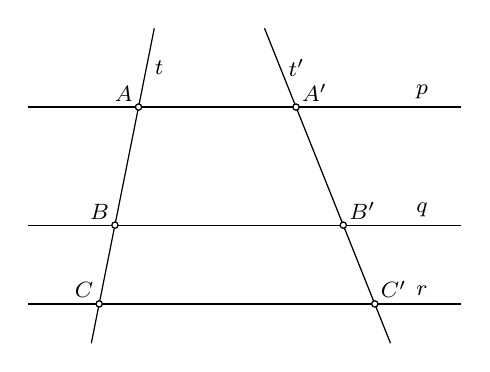
\begin{tikzpicture}
            % \clip (0,0) rectangle (14.000000,10.000000);
            {\footnotesize
            
            % Drawing line p A
            \draw [line width=0.016cm] (1.000000,4.000000) -- (2.360000,4.000000);%
            \draw [line width=0.016cm] (2.440000,4.000000) -- (4.360000,4.000000);%
            \draw [line width=0.016cm] (4.440000,4.000000) -- (6.500000,4.000000);%
            
            % Drawing line Q
            \draw [line width=0.016cm] (1.000000,2.500000) -- (2.060000,2.500000);%
            \draw [line width=0.016cm] (2.140000,2.500000) -- (4.960000,2.500000);%
            \draw [line width=0.016cm] (5.040000,2.500000) -- (6.500000,2.500000);%
            
            % Drawing line T
            \draw [line width=0.016cm] (1.800000,1.000000) -- (1.892155,1.460777);%
            \draw [line width=0.016cm] (1.907845,1.539223) -- (2.092155,2.460777);%
            \draw [line width=0.016cm] (2.107845,2.539223) -- (2.392155,3.960777);%
            \draw [line width=0.016cm] (2.407845,4.039223) -- (2.600000,5.000000);%
            
            % Drawing line R
            \draw [line width=0.016cm] (1.000000,1.500000) -- (1.860000,1.500000);%
            \draw [line width=0.016cm] (1.940000,1.500000) -- (5.360000,1.500000);%
            \draw [line width=0.016cm] (5.440000,1.500000) -- (6.500000,1.500000);%
            
            % Drawing line T'
            \draw [line width=0.016cm] (5.600000,1.000000) -- (5.414856,1.462861);%
            \draw [line width=0.016cm] (5.385144,1.537139) -- (5.014856,2.462861);%
            \draw [line width=0.016cm] (4.985144,2.537139) -- (4.414856,3.962861);%
            \draw [line width=0.016cm] (4.385144,4.037139) -- (4.000000,5.000000);%
            
            % Marking point A by circle
            \draw [line width=0.016cm] (2.400000,4.000000) circle (0.040000);%
            \draw (2.430000,3.970000) node [anchor=south east] { $A$ };%
            
            % Marking point B by circle
            \draw [line width=0.016cm] (2.100000,2.500000) circle (0.040000);%
            \draw (2.130000,2.470000) node [anchor=south east] { $B$ };%
            
            % Marking point C by circle
            \draw [line width=0.016cm] (1.900000,1.500000) circle (0.040000);%
            \draw (1.930000,1.470000) node [anchor=south east] { $C$ };%
            
            % Marking point A' by circle
            \draw [line width=0.016cm] (4.400000,4.000000) circle (0.040000);%
            \draw (4.370000,3.970000) node [anchor=south west] { $A'$ };%
            
            % Marking point B' by circle
            \draw [line width=0.016cm] (5.000000,2.500000) circle (0.040000);%
            \draw (4.970000,2.470000) node [anchor=south west] { $B'$ };%
            
            % Marking point C' by circle
            \draw [line width=0.016cm] (5.400000,1.500000) circle (0.040000);%
            \draw (5.370000,1.470000) node [anchor=south west] { $C'$ };%
            
            % Marking point p
            \draw (6.000000,4.000000) node [anchor=south] { $p$ };%
            
            % Marking point q
            \draw (6.000000,2.500000) node [anchor=south] { $q$ };%
            
            % Marking point r
            \draw (6.000000,1.500000) node [anchor=south] { $r$ };%
            
            % Marking point t
            \draw (2.500000,4.500000) node [anchor=west] { $t$ };%
            
            % Marking point t'
            \draw (4.200000,4.500000) node [anchor=west] { $t'$ };%
            }
        \end{tikzpicture}        
        
        \begin{dokaz}
            \\ 1.\ možnost: \\
            $\frac{|AB|}{|BC|}=\frac{m}{n}\in \QQ; m,n\in\NN \rightarrow \frac{|AB|}{m}=\frac{|BC|}{n}$ --- Daljico $AB$ razdelimo na $m$ skladnih daljic, daljico $BC$ pa na $n$ skladnih daljic. Skozi vse delilne točke potegnemo vzporednice s premico $p$. To po spodnji lemi razdeli $A'B'$ na $m$ skaldnih daljic, $B'C'$ pa na $n$ skladnih daljic in vse te so med sabo skladne: $|A'B'|=md$ in $|B'C'|=nd$ ($d$ dolžina teh daljic).
             $\Rightarrow \frac{|A'B'|}{|B'C'|}=\frac{m}{n}=\frac{|AB|}{|BC|}$.
            \\ 2.\ možnost: 
            \\ 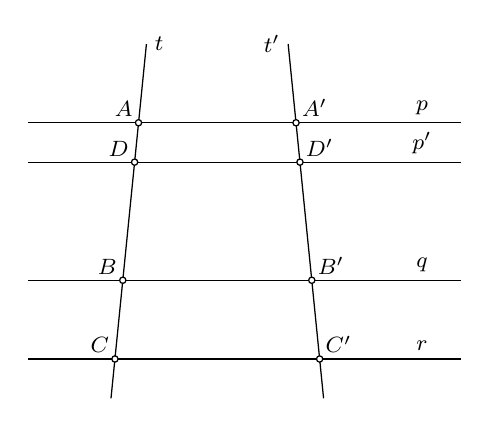
\begin{tikzpicture}
                % \clip (0,0) rectangle (14.000000,10.000000);
                {\footnotesize
                
                % Drawing line p A
                \draw [line width=0.016cm] (1.000000,4.500000) -- (2.360000,4.500000);%
                \draw [line width=0.016cm] (2.440000,4.500000) -- (4.360000,4.500000);%
                \draw [line width=0.016cm] (4.440000,4.500000) -- (6.500000,4.500000);%
                
                % Drawing line Q
                \draw [line width=0.016cm] (1.000000,4.000000) -- (2.310000,4.000000);%
                \draw [line width=0.016cm] (2.390000,4.000000) -- (4.410000,4.000000);%
                \draw [line width=0.016cm] (4.490000,4.000000) -- (6.500000,4.000000);%
                
                % Drawing line T
                \draw [line width=0.016cm] (2.050000,1.000000) -- (2.096020,1.460199);%
                \draw [line width=0.016cm] (2.103980,1.539801) -- (2.196020,2.460199);%
                \draw [line width=0.016cm] (2.203980,2.539801) -- (2.346020,3.960199);%
                \draw [line width=0.016cm] (2.353980,4.039801) -- (2.396020,4.460199);%
                \draw [line width=0.016cm] (2.403980,4.539801) -- (2.500000,5.500000);%
                
                % Drawing line R
                \draw [line width=0.016cm] (1.000000,1.500000) -- (2.060000,1.500000);%
                \draw [line width=0.016cm] (2.140000,1.500000) -- (4.660000,1.500000);%
                \draw [line width=0.016cm] (4.740000,1.500000) -- (6.500000,1.500000);%
                
                % Drawing line T'
                \draw [line width=0.016cm] (4.750000,1.000000) -- (4.703980,1.460199);%
                \draw [line width=0.016cm] (4.696020,1.539801) -- (4.603980,2.460199);%
                \draw [line width=0.016cm] (4.596020,2.539801) -- (4.453980,3.960199);%
                \draw [line width=0.016cm] (4.446020,4.039801) -- (4.403980,4.460199);%
                \draw [line width=0.016cm] (4.396020,4.539801) -- (4.300000,5.500000);%
                
                % Drawing line P'
                \draw [line width=0.016cm] (1.000000,2.500000) -- (2.160000,2.500000);%
                \draw [line width=0.016cm] (2.240000,2.500000) -- (4.560000,2.500000);%
                \draw [line width=0.016cm] (4.640000,2.500000) -- (6.500000,2.500000);%
                
                % Marking point A by circle
                \draw [line width=0.016cm] (2.400000,4.500000) circle (0.040000);%
                \draw (2.430000,4.470000) node [anchor=south east] { $A$ };%
                
                % Marking point B by circle
                \draw [line width=0.016cm] (2.200000,2.500000) circle (0.040000);%
                \draw (2.230000,2.470000) node [anchor=south east] { $B$ };%
                
                % Marking point C by circle
                \draw [line width=0.016cm] (2.100000,1.500000) circle (0.040000);%
                \draw (2.130000,1.470000) node [anchor=south east] { $C$ };%
                
                % Marking point A' by circle
                \draw [line width=0.016cm] (4.400000,4.500000) circle (0.040000);%
                \draw (4.370000,4.470000) node [anchor=south west] { $A'$ };%
                
                % Marking point B' by circle
                \draw [line width=0.016cm] (4.600000,2.500000) circle (0.040000);%
                \draw (4.570000,2.470000) node [anchor=south west] { $B'$ };%
                
                % Marking point C' by circle
                \draw [line width=0.016cm] (4.700000,1.500000) circle (0.040000);%
                \draw (4.670000,1.470000) node [anchor=south west] { $C'$ };%
                
                % Marking point D by circle
                \draw [line width=0.016cm] (2.350000,4.000000) circle (0.040000);%
                \draw (2.380000,3.970000) node [anchor=south east] { $D$ };%
                
                % Marking point D' by circle
                \draw [line width=0.016cm] (4.450000,4.000000) circle (0.040000);%
                \draw (4.420000,3.970000) node [anchor=south west] { $D'$ };%
                
                % Marking point p
                \draw (6.000000,4.500000) node [anchor=south] { $p$ };%
                
                % Marking point q
                \draw (6.000000,2.500000) node [anchor=south] { $q$ };%
                
                % Marking point r
                \draw (6.000000,1.500000) node [anchor=south] { $r$ };%
                
                % Marking point t
                \draw (2.500000,5.500000) node [anchor=west] { $t$ };%
                
                % Marking point t'
                \draw (4.300000,5.500000) node [anchor=east] { $t'$ };%
                
                % Marking point p'
                \draw (6.000000,4.000000) node [anchor=south] { $p'$ };%
                }
                \end{tikzpicture}                  
            \\ Naj bosta $x=\frac{|AB|}{|BC|}$ in $y=\frac{|A'B'|}{|B'C'|}$ iracionalni števili. Če je $x=y$, je `OK'. Sicer: npr. $y<x$. Potem obstaja $\frac{m}{n}\in (y,x)$.  $\frac{|AB|}{|BC|}=x>\frac{m}{n} \Rightarrow |AB|>\frac{m}{n}|BC|$. Potem obstaja točka $D$, da je $A\ast D\ast B$ in $|BD|=\frac{m}{n}|BC|$. Naj bo premica $\tilde{p}$, $\tilde{p}\parallel p$ skozi $D$ in $D'$ presečišče $\tilde{p}$ in $t'$. Ker je $\frac{|DB|}{|BC|}=\frac{m}{n}\in\QQ$, potem je po (1): $\frac{|D'B'|}{|BC|}=\frac{m}{n}$. To nas privede do prostislovja: $|D'B'|=\frac{m}{n}|B'C'|>y|B'C'|=|A'B'|$ (hkrati bi veljalo $B'\ast A'\ast D'$ in $B'\ast D'\ast A'$).
        \end{dokaz}

    \begin{lema}
        Če velja $A\ast B\ast C$, potem je $A'\ast B'\ast C'$.
    \end{lema}

        \begin{dokaz}
            \\ $B$ in $B'$ sta na istem bregu premice $p$, saj $BB'$ oziroma $q$ ne seka premice $p$. Podobno sta $B$ in $B'$ na istem bregu premice $r$.
        \end{dokaz}

    \begin{lema}
        Naj bodo $p, q, \tilde{q}, r$ vzporedne, z morebitno izjemo $q=\tilde{q}$. Naj bosta $t$ in $t'$ sekanti in označimo presečišča $p, q, \tilde{q}, r$ s $t$ oziroma $t'$ z $A, B, C, D$ oziroma $A', B', C', D'$. 
        Če je $AB\cong CD$, potem je $A'B'\cong C'D'$.
    \end{lema}

        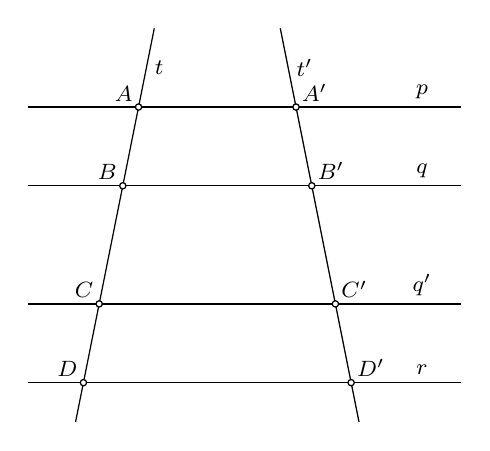
\begin{tikzpicture}
            % \clip (0,0) rectangle (14.000000,10.000000);
            {\footnotesize
            
            % Drawing line p A
            \draw [line width=0.016cm] (1.000000,5.000000) -- (2.360000,5.000000);%
            \draw [line width=0.016cm] (2.440000,5.000000) -- (4.360000,5.000000);%
            \draw [line width=0.016cm] (4.440000,5.000000) -- (6.500000,5.000000);%
            
            % Drawing line Q
            \draw [line width=0.016cm] (1.000000,4.000000) -- (2.160000,4.000000);%
            \draw [line width=0.016cm] (2.240000,4.000000) -- (4.560000,4.000000);%
            \draw [line width=0.016cm] (4.640000,4.000000) -- (6.500000,4.000000);%
            
            % Drawing line T
            \draw [line width=0.016cm] (1.600000,1.000000) -- (1.692155,1.460777);%
            \draw [line width=0.016cm] (1.707845,1.539223) -- (1.892155,2.460777);%
            \draw [line width=0.016cm] (1.907845,2.539223) -- (2.192155,3.960777);%
            \draw [line width=0.016cm] (2.207845,4.039223) -- (2.392155,4.960777);%
            \draw [line width=0.016cm] (2.407845,5.039223) -- (2.600000,6.000000);%
            
            % Drawing line R
            \draw [line width=0.016cm] (1.000000,1.500000) -- (1.660000,1.500000);%
            \draw [line width=0.016cm] (1.740000,1.500000) -- (5.060000,1.500000);%
            \draw [line width=0.016cm] (5.140000,1.500000) -- (6.500000,1.500000);%
            
            % Drawing line T'
            \draw [line width=0.016cm] (5.200000,1.000000) -- (5.107845,1.460777);%
            \draw [line width=0.016cm] (5.092155,1.539223) -- (4.907845,2.460777);%
            \draw [line width=0.016cm] (4.892155,2.539223) -- (4.607845,3.960777);%
            \draw [line width=0.016cm] (4.592155,4.039223) -- (4.407845,4.960777);%
            \draw [line width=0.016cm] (4.392155,5.039223) -- (4.200000,6.000000);%
            
            % Drawing line Q'
            \draw [line width=0.016cm] (1.000000,2.500000) -- (1.860000,2.500000);%
            \draw [line width=0.016cm] (1.940000,2.500000) -- (4.860000,2.500000);%
            \draw [line width=0.016cm] (4.940000,2.500000) -- (6.500000,2.500000);%
            
            % Marking point A by circle
            \draw [line width=0.016cm] (2.400000,5.000000) circle (0.040000);%
            \draw (2.430000,4.970000) node [anchor=south east] { $A$ };%
            
            % Marking point B by circle
            \draw [line width=0.016cm] (2.200000,4.000000) circle (0.040000);%
            \draw (2.230000,3.970000) node [anchor=south east] { $B$ };%
            
            % Marking point C by circle
            \draw [line width=0.016cm] (1.900000,2.500000) circle (0.040000);%
            \draw (1.930000,2.470000) node [anchor=south east] { $C$ };%
            
            % Marking point A' by circle
            \draw [line width=0.016cm] (4.400000,5.000000) circle (0.040000);%
            \draw (4.370000,4.970000) node [anchor=south west] { $A'$ };%
            
            % Marking point B' by circle
            \draw [line width=0.016cm] (4.600000,4.000000) circle (0.040000);%
            \draw (4.570000,3.970000) node [anchor=south west] { $B'$ };%
            
            % Marking point C' by circle
            \draw [line width=0.016cm] (4.900000,2.500000) circle (0.040000);%
            \draw (4.870000,2.470000) node [anchor=south west] { $C'$ };%
            
            % Marking point D by circle
            \draw [line width=0.016cm] (1.700000,1.500000) circle (0.040000);%
            \draw (1.730000,1.470000) node [anchor=south east] { $D$ };%
            
            % Marking point D' by circle
            \draw [line width=0.016cm] (5.100000,1.500000) circle (0.040000);%
            \draw (5.070000,1.470000) node [anchor=south west] { $D'$ };%
            
            % Marking point p
            \draw (6.000000,5.000000) node [anchor=south] { $p$ };%
            
            % Marking point q
            \draw (6.000000,4.000000) node [anchor=south] { $q$ };%
            
            % Marking point r
            \draw (6.000000,1.500000) node [anchor=south] { $r$ };%
            
            % Marking point t
            \draw (2.500000,5.500000) node [anchor=west] { $t$ };%
            
            % Marking point t'
            \draw (4.300000,5.500000) node [anchor=west] { $t'$ };%
            
            % Marking point q'
            \draw (6.000000,2.500000) node [anchor=south] { $q'$ };%
            }
        \end{tikzpicture}

        \begin{dokaz}
            \\ Naj bo $s$ oziroma $s'$ vzporednica k $t$ (oziroma $t'$) skozi $A'$ oziroma $C'$. 
            Štirikotnika $AA'EB$ in $CC'FD$ sta paralelograma, zato je $A'E\cong AB$ in $C'F\cong CD$ ter iz tega sledi $A'E\cong C'F$.
            Ker je $s\parallel t, \tilde{s}\parallel t \Rightarrow s\parallel\tilde{s}$, sledi, da je: $\angle EA'B'\cong\angle FC'D'$. 
            Ker je $q\parallel r$, ju prečnica $t'$ seka pod enakim kotom, torej je: $\angle FD'C'\cong \angle EB'A'$. 
            Po SKK sta trikotnika $\triangle EA'B'$ in $\triangle FC'D'$ skladna. 
            $\Rightarrow A'B'\cong C'D'$
            \\ 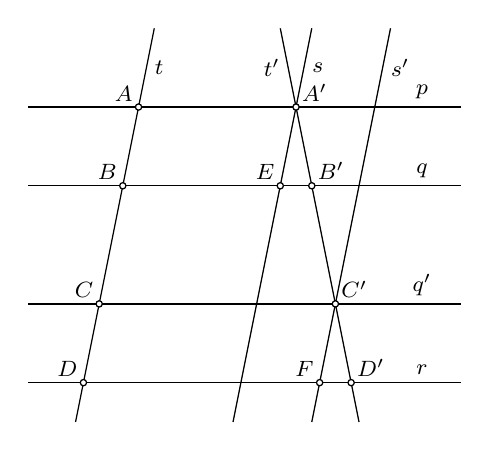
\begin{tikzpicture}
                % \clip (0,0) rectangle (14.000000,10.000000);
                {\footnotesize
                
                % Drawing line p A
                \draw [line width=0.016cm] (1.000000,5.000000) -- (2.360000,5.000000);%
                \draw [line width=0.016cm] (2.440000,5.000000) -- (4.360000,5.000000);%
                \draw [line width=0.016cm] (4.440000,5.000000) -- (6.500000,5.000000);%
                
                % Drawing line Q
                \draw [line width=0.016cm] (1.000000,4.000000) -- (2.160000,4.000000);%
                \draw [line width=0.016cm] (2.240000,4.000000) -- (4.160000,4.000000);%
                \draw [line width=0.016cm] (4.240000,4.000000) -- (4.560000,4.000000);%
                \draw [line width=0.016cm] (4.640000,4.000000) -- (6.500000,4.000000);%
                
                % Drawing line T
                \draw [line width=0.016cm] (1.600000,1.000000) -- (1.692155,1.460777);%
                \draw [line width=0.016cm] (1.707845,1.539223) -- (1.892155,2.460777);%
                \draw [line width=0.016cm] (1.907845,2.539223) -- (2.192155,3.960777);%
                \draw [line width=0.016cm] (2.207845,4.039223) -- (2.392155,4.960777);%
                \draw [line width=0.016cm] (2.407845,5.039223) -- (2.600000,6.000000);%
                
                % Drawing line R
                \draw [line width=0.016cm] (1.000000,1.500000) -- (1.660000,1.500000);%
                \draw [line width=0.016cm] (1.740000,1.500000) -- (4.660000,1.500000);%
                \draw [line width=0.016cm] (4.740000,1.500000) -- (5.060000,1.500000);%
                \draw [line width=0.016cm] (5.140000,1.500000) -- (6.500000,1.500000);%
                
                % Drawing line T'
                \draw [line width=0.016cm] (5.200000,1.000000) -- (5.107845,1.460777);%
                \draw [line width=0.016cm] (5.092155,1.539223) -- (4.907845,2.460777);%
                \draw [line width=0.016cm] (4.892155,2.539223) -- (4.607845,3.960777);%
                \draw [line width=0.016cm] (4.592155,4.039223) -- (4.407845,4.960777);%
                \draw [line width=0.016cm] (4.392155,5.039223) -- (4.200000,6.000000);%
                
                % Drawing line Q'
                \draw [line width=0.016cm] (1.000000,2.500000) -- (1.860000,2.500000);%
                \draw [line width=0.016cm] (1.940000,2.500000) -- (4.860000,2.500000);%
                \draw [line width=0.016cm] (4.940000,2.500000) -- (6.500000,2.500000);%
                
                % Drawing line S
                \draw [line width=0.016cm] (3.600000,1.000000) -- (4.192155,3.960777);%
                \draw [line width=0.016cm] (4.207845,4.039223) -- (4.392155,4.960777);%
                \draw [line width=0.016cm] (4.407845,5.039223) -- (4.600000,6.000000);%
                
                % Drawing line S'
                \draw [line width=0.016cm] (4.600000,1.000000) -- (4.692155,1.460777);%
                \draw [line width=0.016cm] (4.707845,1.539223) -- (4.892155,2.460777);%
                \draw [line width=0.016cm] (4.907845,2.539223) -- (5.600000,6.000000);%
                
                % Marking point A by circle
                \draw [line width=0.016cm] (2.400000,5.000000) circle (0.040000);%
                \draw (2.430000,4.970000) node [anchor=south east] { $A$ };%
                
                % Marking point B by circle
                \draw [line width=0.016cm] (2.200000,4.000000) circle (0.040000);%
                \draw (2.230000,3.970000) node [anchor=south east] { $B$ };%
                
                % Marking point C by circle
                \draw [line width=0.016cm] (1.900000,2.500000) circle (0.040000);%
                \draw (1.930000,2.470000) node [anchor=south east] { $C$ };%
                
                % Marking point A' by circle
                \draw [line width=0.016cm] (4.400000,5.000000) circle (0.040000);%
                \draw (4.370000,4.970000) node [anchor=south west] { $A'$ };%
                
                % Marking point B' by circle
                \draw [line width=0.016cm] (4.600000,4.000000) circle (0.040000);%
                \draw (4.570000,3.970000) node [anchor=south west] { $B'$ };%
                
                % Marking point C' by circle
                \draw [line width=0.016cm] (4.900000,2.500000) circle (0.040000);%
                \draw (4.870000,2.470000) node [anchor=south west] { $C'$ };%
                
                % Marking point D by circle
                \draw [line width=0.016cm] (1.700000,1.500000) circle (0.040000);%
                \draw (1.730000,1.470000) node [anchor=south east] { $D$ };%
                
                % Marking point D' by circle
                \draw [line width=0.016cm] (5.100000,1.500000) circle (0.040000);%
                \draw (5.070000,1.470000) node [anchor=south west] { $D'$ };%
                
                % Marking point F by circle
                \draw [line width=0.016cm] (4.700000,1.500000) circle (0.040000);%
                \draw (4.730000,1.470000) node [anchor=south east] { $F$ };%
                
                % Marking point E by circle
                \draw [line width=0.016cm] (4.200000,4.000000) circle (0.040000);%
                \draw (4.230000,3.970000) node [anchor=south east] { $E$ };%
                
                % Marking point p
                \draw (6.000000,5.000000) node [anchor=south] { $p$ };%
                
                % Marking point q
                \draw (6.000000,4.000000) node [anchor=south] { $q$ };%
                
                % Marking point r
                \draw (6.000000,1.500000) node [anchor=south] { $r$ };%
                
                % Marking point t
                \draw (2.500000,5.500000) node [anchor=west] { $t$ };%
                
                % Marking point t'
                \draw (4.300000,5.500000) node [anchor=east] { $t'$ };%
                
                % Marking point q'
                \draw (6.000000,2.500000) node [anchor=south] { $q'$ };%
                
                % Marking point s
                \draw (4.500000,5.500000) node [anchor=west] { $s$ };%
                
                % Marking point s'
                \draw (5.500000,5.500000) node [anchor=west] { $s'$ };%
                }
                \end{tikzpicture}  
        \end{dokaz}

\section{Evklidovi elementi}

    \subsection*{Knjiga 1}

        Preostale trditve iz Knjige 1 se večinoma nanašajo na paralelograme ter na ploščine trikotnikov in paralelogramov.

        \begin{trditev}[I.48 -- obrat Pitagorovega izreka]
            Če v trikotniku s stranicami $a, b, c$ velja $a^2+b^2=c^2$, potem je trikotnik pravokoten.
        \end{trditev}

            \begin{dokaz}
                \\ Dan imamo trikotnik $\triangle ABC$. Konstruiramo pravokoten trikotnik s katetama $a$ in $b$. Po Pitagorovem izreku je hipotenuza dolžine $\sqrt{a^2+b^2}=c$. Po kriteriju SSS sta trikotnika skladna.
            \end{dokaz}


    \subsection*{Knjiga 2}

        Knjiga 2 je posvečena geometrijski algebri.
        
        \noindent Za dolžino $a$ predstavlja $a^2$ ploščino kvadrata.
        Za dolžini $a$ in $b$ predstavlja $ab$ ploščino pravokotnika s stranicama $a$ in $b$.

        \begin{trditev}[II.1]
            $(a+b)c=ac+bc$
        \end{trditev}

            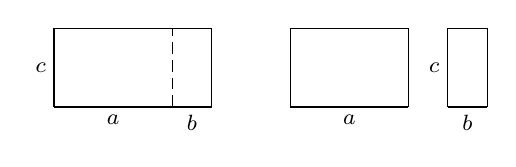
\begin{tikzpicture}
                % \clip (0,0) rectangle (14.000000,10.000000);
                {\footnotesize
                
                % Drawing segment A C
                \draw [line width=0.016cm] (1.500000,1.500000) -- (3.500000,1.500000);%
                
                % Drawing segment D E
                \draw [line width=0.016cm] (4.500000,1.500000) -- (6.000000,1.500000);%
                
                % Drawing segment F G
                \draw [line width=0.016cm] (6.500000,1.500000) -- (7.000000,1.500000);%
                
                % Drawing segment H J
                \draw [line width=0.016cm] (1.500000,2.500000) -- (3.500000,2.500000);%
                
                % Drawing segment K L
                \draw [line width=0.016cm] (4.500000,2.500000) -- (6.000000,2.500000);%
                
                % Drawing segment M N
                \draw [line width=0.016cm] (6.500000,2.500000) -- (7.000000,2.500000);%
                
                % Drawing segment A H
                \draw [line width=0.016cm] (1.500000,1.500000) -- (1.500000,2.500000);%
                
                % Drawing segment B I
                \draw [line width=0.016cm] (3.000000,1.500000) -- (3.000000,1.650000);%
                \draw [line width=0.016cm] (3.000000,1.725000) -- (3.000000,1.875000);%
                \draw [line width=0.016cm] (3.000000,1.950000) -- (3.000000,2.100000);%
                \draw [line width=0.016cm] (3.000000,2.175000) -- (3.000000,2.325000);%
                \draw [line width=0.016cm] (3.000000,2.400000) -- (3.000000,2.500000);%
                
                % Drawing segment C J
                \draw [line width=0.016cm] (3.500000,1.500000) -- (3.500000,2.500000);%
                
                % Drawing segment D K
                \draw [line width=0.016cm] (4.500000,1.500000) -- (4.500000,2.500000);%
                
                % Drawing segment E L
                \draw [line width=0.016cm] (6.000000,1.500000) -- (6.000000,2.500000);%
                
                % Drawing segment F M
                \draw [line width=0.016cm] (6.500000,1.500000) -- (6.500000,2.500000);%
                
                % Drawing segment G N
                \draw [line width=0.016cm] (7.000000,1.500000) -- (7.000000,2.500000);%
                
                % Marking point c
                \draw (1.500000,2.000000) node [anchor=east] { $c$ };%
                
                % Marking point a
                \draw (2.250000,1.500000) node [anchor=north] { $a$ };%
                
                % Marking point b
                \draw (3.250000,1.500000) node [anchor=north] { $b$ };%
                
                % Marking point c
                \draw (6.500000,2.000000) node [anchor=east] { $c$ };%
                
                % Marking point a
                \draw (5.250000,1.500000) node [anchor=north] { $a$ };%
                
                % Marking point b
                \draw (6.750000,1.500000) node [anchor=north] { $b$ };%
                }
            \end{tikzpicture}

        \begin{trditev}[II.4]
            ${(a+b)}^2=a^2+2ab+b^2$
        \end{trditev}

            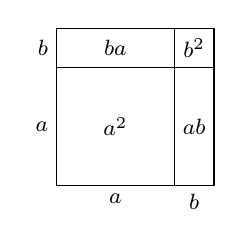
\begin{tikzpicture}
                % \clip (0,0) rectangle (14.000000,10.000000);
                {\footnotesize
                
                % Drawing segment A C
                \draw [line width=0.016cm] (1.500000,1.500000) -- (3.500000,1.500000);%
                
                % Drawing segment F H
                \draw [line width=0.016cm] (1.500000,3.500000) -- (3.500000,3.500000);%
                
                % Drawing segment A F
                \draw [line width=0.016cm] (1.500000,1.500000) -- (1.500000,3.500000);%
                
                % Drawing segment C H
                \draw [line width=0.016cm] (3.500000,1.500000) -- (3.500000,3.500000);%
                
                % Drawing segment G B
                \draw [line width=0.016cm] (3.000000,3.500000) -- (3.000000,1.500000);%
                
                % Drawing segment D E
                \draw [line width=0.016cm] (1.500000,3.000000) -- (3.500000,3.000000);%
                
                % Marking point a
                \draw (2.250000,1.500000) node [anchor=north] { $a$ };%
                
                % Marking point b
                \draw (3.250000,1.500000) node [anchor=north] { $b$ };%
                
                % Marking point a
                \draw (1.500000,2.250000) node [anchor=east] { $a$ };%
                
                % Marking point b
                \draw (1.500000,3.250000) node [anchor=east] { $b$ };%
                
                % Marking point ba
                \draw (2.250000,3.250000) node  { $ba$ };%
                
                % Marking point b^2
                \draw (3.250000,3.250000) node  { $b^2$ };%
                
                % Marking point a^2
                \draw (2.250000,2.250000) node  { $a^2$ };%
                
                % Marking point ab
                \draw (3.250000,2.250000) node  { $ab$ };%
                }
            \end{tikzpicture}

        \begin{trditev}[II.11]
            Razdelitev dane daljice tako, da je pravokotnik na daljici in enem od delov daljice enak kvadratu na drugem delu daljice.
        \end{trditev}

        $ax=y^2$ in $x+y=a$ \ldots razmerje zlatega reza: $\frac{a}{y}=\frac{y}{x}=\frac{y}{a-y}$.

        Iz $a^2-ay=y^2$ dobimo: $y=\frac{-a\pm\sqrt{a^2+4a^2}}{2}=a\left(\frac{-1\pm\sqrt{5}}{2}\right)$ Sledi: $\frac{a}{y}=\frac{1+\sqrt{5}}{2}=\tau$

        Geometrijska konstrukcija $\tau$:

            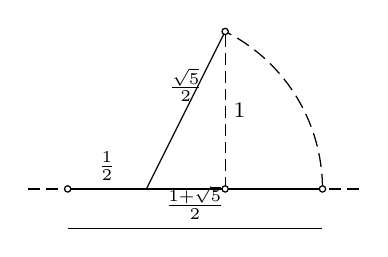
\begin{tikzpicture}
                % \clip (0,0) rectangle (14.000000,10.000000);
                {\footnotesize
                
                % Marking point A by circle
                \draw [line width=0.016cm] (1.500000,2.000000) circle (0.040000);%
                
                % Marking point B by circle
                \draw [line width=0.016cm] (3.500000,2.000000) circle (0.040000);%
                
                % Marking point C by circle
                \draw [line width=0.016cm] (3.500000,4.000000) circle (0.040000);%
                
                % Marking point E by circle
                \draw [line width=0.016cm] (4.736068,2.000000) circle (0.040000);%
                
                % Drawing line A B
                \draw [line width=0.016cm] (1.000000,2.000000) -- (1.150000,2.000000);%
                \draw [line width=0.016cm] (1.225000,2.000000) -- (1.375000,2.000000);%
                \draw [line width=0.016cm] (1.450000,2.000000) -- (1.460000,2.000000);%
                \draw [line width=0.016cm] (1.540000,2.000000) -- (1.600000,2.000000);%
                \draw [line width=0.016cm] (1.675000,2.000000) -- (1.825000,2.000000);%
                \draw [line width=0.016cm] (1.900000,2.000000) -- (2.050000,2.000000);%
                \draw [line width=0.016cm] (2.125000,2.000000) -- (2.275000,2.000000);%
                \draw [line width=0.016cm] (2.350000,2.000000) -- (2.500000,2.000000);%
                \draw [line width=0.016cm] (2.575000,2.000000) -- (2.725000,2.000000);%
                \draw [line width=0.016cm] (2.800000,2.000000) -- (2.950000,2.000000);%
                \draw [line width=0.016cm] (3.025000,2.000000) -- (3.175000,2.000000);%
                \draw [line width=0.016cm] (3.250000,2.000000) -- (3.400000,2.000000);%
                \draw [line width=0.016cm] (3.540000,2.000000) -- (3.625000,2.000000);%
                \draw [line width=0.016cm] (3.700000,2.000000) -- (3.850000,2.000000);%
                \draw [line width=0.016cm] (3.925000,2.000000) -- (4.075000,2.000000);%
                \draw [line width=0.016cm] (4.150000,2.000000) -- (4.300000,2.000000);%
                \draw [line width=0.016cm] (4.375000,2.000000) -- (4.525000,2.000000);%
                \draw [line width=0.016cm] (4.600000,2.000000) -- (4.696068,2.000000);%
                \draw [line width=0.016cm] (4.825000,2.000000) -- (4.975000,2.000000);%
                \draw [line width=0.016cm] (5.050000,2.000000) -- (5.200000,2.000000);%
                
                % Drawing arc D C -63.00
                \draw [line width=0.016cm] (4.735710,2.039998) -- (4.734706,2.078038) arc (2:2:2.236068 and 2.236068) -- (4.733613,2.104747);%
                \draw [line width=0.016cm] (4.733613,2.104747) -- (4.733004,2.117027) arc (3:4:2.236068 and 2.236068) -- (4.727779,2.192357);%
                \draw [line width=0.016cm] (4.718509,2.279671) -- (4.714307,2.311200) arc (8:9:2.236068 and 2.236068) -- (4.705819,2.366554);%
                \draw [line width=0.016cm] (4.705819,2.366554) -- (4.702097,2.388289) arc (10:11:2.236068 and 2.236068) -- (4.689728,2.452871);%
                \draw [line width=0.016cm] (4.670260,2.538490) -- (4.669647,2.540954) arc (14:16:2.236068 and 2.236068) -- (4.647446,2.623279);%
                \draw [line width=0.016cm] (4.647446,2.623279) -- (4.638362,2.653763) arc (17:18:2.236068 and 2.236068) -- (4.621320,2.707107);%
                \draw [line width=0.016cm] (4.591924,2.789844) -- (4.587549,2.801335) arc (21:22:2.236068 and 2.236068) -- (4.559302,2.871364);%
                \draw [line width=0.016cm] (4.559302,2.871364) -- (4.558311,2.873701) arc (23:25:2.236068 and 2.236068) -- (4.523505,2.951540);%
                \draw [line width=0.016cm] (4.484587,3.030249) -- (4.474331,3.049770) arc (28:29:2.236068 and 2.236068) -- (4.442610,3.107369);%
                \draw [line width=0.016cm] (4.442610,3.107369) -- (4.436492,3.118034) arc (30:31:2.236068 and 2.236068) -- (4.397637,3.182782);%
                \draw [line width=0.016cm] (4.349738,3.256371) -- (4.331680,3.282556) arc (35:36:2.236068 and 2.236068) -- (4.298987,3.328023);%
                \draw [line width=0.016cm] (4.298987,3.328023) -- (4.285803,3.345699) arc (37:38:2.236068 and 2.236068) -- (4.245463,3.397627);%
                \draw [line width=0.016cm] (4.189246,3.465076) -- (4.187582,3.466993) arc (41:43:2.236068 and 2.236068) -- (4.130425,3.530266);%
                \draw [line width=0.016cm] (4.130425,3.530266) -- (4.108493,3.553303) arc (44:45:2.236068 and 2.236068) -- (4.069090,3.593096);%
                \draw [line width=0.016cm] (4.005336,3.653470) -- (3.996222,3.661722) arc (48:49:2.236068 and 2.236068) -- (3.939261,3.711294);%
                \draw [line width=0.016cm] (3.939261,3.711294) -- (3.937317,3.712927) arc (50:52:2.236068 and 2.236068) -- (3.870966,3.766480);%
                \draw [line width=0.016cm] (3.800557,3.818942) -- (3.782556,3.831680) arc (55:56:2.236068 and 2.236068) -- (3.728143,3.868600);%
                \draw [line width=0.016cm] (3.728143,3.868600) -- (3.717850,3.875324) arc (57:58:2.236068 and 2.236068) -- (3.653836,3.915376);%
                \draw [line width=0.016cm] (3.577749,3.959198) -- (3.549770,3.974331) arc (62:62:2.236068 and 2.236068) -- (3.535616,3.981792);%
                
                % Drawing segment D C
                \draw [line width=0.016cm] (2.500000,2.000000) -- (3.482111,3.964223);%
                
                % Drawing segment B C
                \draw [line width=0.016cm] (3.500000,2.040000) -- (3.500000,2.150000);%
                \draw [line width=0.016cm] (3.500000,2.225000) -- (3.500000,2.375000);%
                \draw [line width=0.016cm] (3.500000,2.450000) -- (3.500000,2.600000);%
                \draw [line width=0.016cm] (3.500000,2.675000) -- (3.500000,2.825000);%
                \draw [line width=0.016cm] (3.500000,2.900000) -- (3.500000,3.050000);%
                \draw [line width=0.016cm] (3.500000,3.125000) -- (3.500000,3.275000);%
                \draw [line width=0.016cm] (3.500000,3.350000) -- (3.500000,3.500000);%
                \draw [line width=0.016cm] (3.500000,3.575000) -- (3.500000,3.725000);%
                \draw [line width=0.016cm] (3.500000,3.800000) -- (3.500000,3.950000);%
                
                % Drawing segment G H
                \draw [line width=0.016cm] (1.500000,1.500000) -- (4.730000,1.500000);%
                
                % Marking point \frac{1+\sqrt{5}}{2}
                \draw (3.115000,1.500000) node [anchor=south] { $\frac{1+\sqrt{5}}{2}$ };%
                
                % Marking point \frac{\sqrt{5}}{2}
                \draw (3.000000,3.000000) node [anchor=south] { $\frac{\sqrt{5}}{2}$ };%
                
                % Marking point 1
                \draw (3.500000,3.000000) node [anchor=west] { $1$ };%
                
                % Marking point \frac{1}{2}
                \draw (2.000000,2.000000) node [anchor=south] { $\frac{1}{2}$ };%
                
                % Drawing segment A E
                \draw [line width=0.032cm] (1.540000,2.000000) -- (3.460000,2.000000);%
                \draw [line width=0.032cm] (3.540000,2.000000) -- (4.696068,2.000000);%
                }
            \end{tikzpicture}


    \subsection*{Knjiga 3}

        Knjiga 3 govori o krožnicah.

        \begin{trditev}[III.1]
            Konstrukcija središča dane krožnice.
        \end{trditev}

            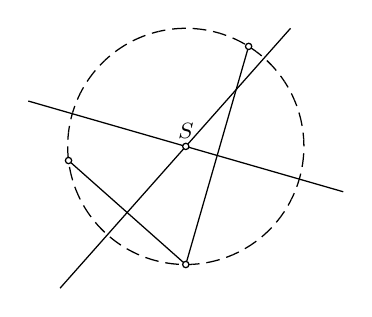
\begin{tikzpicture}
                % \clip (0,0) rectangle (14.000000,10.000000);
                {\footnotesize
                
                % Drawing segment R Q
                \draw [line width=0.016cm] (3.786945,4.231669) -- (3.011073,1.538437);%
                
                % Drawing segment P Q
                \draw [line width=0.016cm] (1.540677,2.794193) -- (2.970073,1.526540);%
                
                % Drawing circle S Q
                \draw [line width=0.016cm] (3.039996,1.500533) -- (3.052349,1.500914) arc (272:273:1.500000 and 1.500000) -- (3.087217,1.502538);%
                \draw [line width=0.016cm] (3.087217,1.502538) -- (3.104634,1.503654) arc (274:276:1.500000 and 1.500000) -- (3.174139,1.510142);%
                \draw [line width=0.016cm] (3.260472,1.522788) -- (3.260472,1.522788) arc (280:283:1.500000 and 1.500000) -- (3.345923,1.540433);%
                \draw [line width=0.016cm] (3.345923,1.540433) -- (3.362882,1.544556) arc (284:286:1.500000 and 1.500000) -- (3.430204,1.563016);%
                \draw [line width=0.016cm] (3.513030,1.590461) -- (3.513030,1.590461) arc (290:293:1.500000 and 1.500000) -- (3.594119,1.622676);%
                \draw [line width=0.016cm] (3.594119,1.622676) -- (3.610105,1.629682) arc (294:296:1.500000 and 1.500000) -- (3.673198,1.659551);%
                \draw [line width=0.016cm] (3.750000,1.700962) -- (3.750000,1.700962) arc (300:303:1.500000 and 1.500000) -- (3.824263,1.746768);%
                \draw [line width=0.016cm] (3.824263,1.746768) -- (3.838789,1.756443) arc (304:306:1.500000 and 1.500000) -- (3.895737,1.796815);%
                \draw [line width=0.016cm] (3.964181,1.850933) -- (3.964181,1.850933) arc (310:313:1.500000 and 1.500000) -- (4.029362,1.908939);%
                \draw [line width=0.016cm] (4.029362,1.908939) -- (4.041987,1.920990) arc (314:316:1.500000 and 1.500000) -- (4.091060,1.970637);%
                \draw [line width=0.016cm] (4.149066,2.035818) -- (4.149066,2.035818) arc (320:323:1.500000 and 1.500000) -- (4.203184,2.104262);%
                \draw [line width=0.016cm] (4.203184,2.104262) -- (4.213525,2.118322) arc (324:326:1.500000 and 1.500000) -- (4.253231,2.175736);%
                \draw [line width=0.016cm] (4.299038,2.250000) -- (4.299038,2.250000) arc (330:333:1.500000 and 1.500000) -- (4.340449,2.326801);%
                \draw [line width=0.016cm] (4.340449,2.326801) -- (4.348191,2.342443) arc (334:336:1.500000 and 1.500000) -- (4.377324,2.405880);%
                \draw [line width=0.016cm] (4.409539,2.486969) -- (4.409539,2.486969) arc (340:343:1.500000 and 1.500000) -- (4.436984,2.569795);%
                \draw [line width=0.016cm] (4.436984,2.569795) -- (4.441892,2.586544) arc (344:346:1.500000 and 1.500000) -- (4.459567,2.654076);%
                \draw [line width=0.016cm] (4.477212,2.739527) -- (4.477212,2.739527) arc (350:353:1.500000 and 1.500000) -- (4.489857,2.825860);%
                \draw [line width=0.016cm] (4.489857,2.825860) -- (4.491783,2.843207) arc (354:356:1.500000 and 1.500000) -- (4.497462,2.912782);%
                \draw [line width=0.016cm] (4.500000,2.999999) -- (4.500000,3.000000) arc (360:360:1.500000 and 1.500000) --(4.500000,3.000000) arc (0:3:1.500000 and 1.500000) -- (4.497462,3.087217);%
                \draw [line width=0.016cm] (4.497462,3.087217) -- (4.496346,3.104635) arc (4:6:1.500000 and 1.500000) -- (4.489858,3.174139);%
                \draw [line width=0.016cm] (4.477212,3.260472) -- (4.477212,3.260472) arc (10:13:1.500000 and 1.500000) -- (4.459567,3.345924);%
                \draw [line width=0.016cm] (4.459567,3.345924) -- (4.455444,3.362883) arc (14:16:1.500000 and 1.500000) -- (4.436984,3.430205);%
                \draw [line width=0.016cm] (4.409539,3.513030) -- (4.409539,3.513030) arc (20:23:1.500000 and 1.500000) -- (4.377324,3.594120);%
                \draw [line width=0.016cm] (4.377324,3.594120) -- (4.370318,3.610105) arc (24:26:1.500000 and 1.500000) -- (4.340449,3.673199);%
                \draw [line width=0.016cm] (4.299038,3.750000) -- (4.299038,3.750000) arc (30:33:1.500000 and 1.500000) -- (4.253232,3.824263);%
                \draw [line width=0.016cm] (4.253232,3.824263) -- (4.243556,3.838789) arc (34:36:1.500000 and 1.500000) -- (4.203185,3.895738);%
                \draw [line width=0.016cm] (4.149067,3.964181) -- (4.149067,3.964181) arc (40:43:1.500000 and 1.500000) -- (4.091061,4.029362);%
                \draw [line width=0.016cm] (4.091061,4.029362) -- (4.079010,4.041988) arc (44:46:1.500000 and 1.500000) -- (4.029363,4.091060);%
                \draw [line width=0.016cm] (3.964182,4.149067) -- (3.964181,4.149067) arc (50:53:1.500000 and 1.500000) -- (3.895738,4.203185);%
                \draw [line width=0.016cm] (3.895738,4.203185) -- (3.881678,4.213525) arc (54:56:1.500000 and 1.500000) -- (3.831601,4.248375);%
                \draw [line width=0.016cm] (3.750000,4.299038) -- (3.750000,4.299038) arc (60:63:1.500000 and 1.500000) -- (3.673199,4.340449);%
                \draw [line width=0.016cm] (3.673199,4.340449) -- (3.657557,4.348191) arc (64:66:1.500000 and 1.500000) -- (3.594120,4.377324);%
                \draw [line width=0.016cm] (3.513030,4.409539) -- (3.513030,4.409539) arc (70:73:1.500000 and 1.500000) -- (3.430205,4.436984);%
                \draw [line width=0.016cm] (3.430205,4.436984) -- (3.413456,4.441893) arc (74:76:1.500000 and 1.500000) -- (3.345924,4.459567);%
                \draw [line width=0.016cm] (3.260472,4.477212) -- (3.260472,4.477212) arc (80:83:1.500000 and 1.500000) -- (3.174140,4.489858);%
                \draw [line width=0.016cm] (3.174140,4.489858) -- (3.156793,4.491783) arc (84:86:1.500000 and 1.500000) -- (3.087217,4.497462);%
                \draw [line width=0.016cm] (3.000000,4.500000) -- (3.000000,4.500000) arc (90:93:1.500000 and 1.500000) -- (2.912783,4.497462);%
                \draw [line width=0.016cm] (2.912783,4.497462) -- (2.895365,4.496346) arc (94:96:1.500000 and 1.500000) -- (2.825861,4.489858);%
                \draw [line width=0.016cm] (2.739528,4.477212) -- (2.739528,4.477212) arc (100:103:1.500000 and 1.500000) -- (2.654076,4.459567);%
                \draw [line width=0.016cm] (2.654076,4.459567) -- (2.637117,4.455444) arc (104:106:1.500000 and 1.500000) -- (2.569795,4.436984);%
                \draw [line width=0.016cm] (2.486970,4.409539) -- (2.486970,4.409539) arc (110:113:1.500000 and 1.500000) -- (2.405881,4.377324);%
                \draw [line width=0.016cm] (2.405881,4.377324) -- (2.389895,4.370318) arc (114:116:1.500000 and 1.500000) -- (2.326801,4.340449);%
                \draw [line width=0.016cm] (2.250000,4.299038) -- (2.250000,4.299038) arc (120:123:1.500000 and 1.500000) -- (2.175737,4.253232);%
                \draw [line width=0.016cm] (2.175737,4.253232) -- (2.161211,4.243556) arc (124:126:1.500000 and 1.500000) -- (2.104262,4.203185);%
                \draw [line width=0.016cm] (2.035819,4.149067) -- (2.035819,4.149067) arc (130:133:1.500000 and 1.500000) -- (1.970638,4.091061);%
                \draw [line width=0.016cm] (1.970638,4.091061) -- (1.958013,4.079010) arc (134:136:1.500000 and 1.500000) -- (1.908940,4.029363);%
                \draw [line width=0.016cm] (1.850934,3.964182) -- (1.850933,3.964182) arc (140:143:1.500000 and 1.500000) -- (1.796815,3.895738);%
                \draw [line width=0.016cm] (1.796815,3.895738) -- (1.786475,3.881678) arc (144:146:1.500000 and 1.500000) -- (1.746768,3.824264);%
                \draw [line width=0.016cm] (1.700962,3.750000) -- (1.700962,3.750000) arc (150:153:1.500000 and 1.500000) -- (1.659551,3.673199);%
                \draw [line width=0.016cm] (1.659551,3.673199) -- (1.651809,3.657557) arc (154:156:1.500000 and 1.500000) -- (1.622676,3.594120);%
                \draw [line width=0.016cm] (1.590461,3.513031) -- (1.590461,3.513030) arc (160:163:1.500000 and 1.500000) -- (1.563016,3.430205);%
                \draw [line width=0.016cm] (1.563016,3.430205) -- (1.558108,3.413456) arc (164:166:1.500000 and 1.500000) -- (1.540433,3.345924);%
                \draw [line width=0.016cm] (1.522788,3.260473) -- (1.522788,3.260472) arc (170:173:1.500000 and 1.500000) -- (1.510143,3.174140);%
                \draw [line width=0.016cm] (1.510143,3.174140) -- (1.508217,3.156793) arc (174:176:1.500000 and 1.500000) -- (1.502538,3.087218);%
                \draw [line width=0.016cm] (1.500000,3.000000) -- (1.500000,3.000000) arc (180:183:1.500000 and 1.500000) -- (1.502538,2.912783);%
                \draw [line width=0.016cm] (1.502538,2.912784) -- (1.503654,2.895366) arc (184:185:1.500000 and 1.500000) -- (1.506500,2.860507);%
                \draw [line width=0.016cm] (1.522788,2.739529) -- (1.522788,2.739528) arc (190:193:1.500000 and 1.500000) -- (1.540433,2.654077);%
                \draw [line width=0.016cm] (1.540433,2.654077) -- (1.544556,2.637117) arc (194:196:1.500000 and 1.500000) -- (1.563015,2.569796);%
                \draw [line width=0.016cm] (1.590461,2.486971) -- (1.590461,2.486970) arc (200:203:1.500000 and 1.500000) -- (1.622676,2.405881);%
                \draw [line width=0.016cm] (1.622676,2.405881) -- (1.629682,2.389895) arc (204:206:1.500000 and 1.500000) -- (1.659551,2.326802);%
                \draw [line width=0.016cm] (1.700961,2.250001) -- (1.700962,2.250000) arc (210:213:1.500000 and 1.500000) -- (1.746768,2.175737);%
                \draw [line width=0.016cm] (1.746768,2.175737) -- (1.756443,2.161211) arc (214:216:1.500000 and 1.500000) -- (1.796815,2.104263);%
                \draw [line width=0.016cm] (1.850933,2.035819) -- (1.850933,2.035819) arc (220:223:1.500000 and 1.500000) -- (1.908939,1.970638);%
                \draw [line width=0.016cm] (1.908939,1.970638) -- (1.920990,1.958013) arc (224:226:1.500000 and 1.500000) -- (1.970637,1.908940);%
                \draw [line width=0.016cm] (2.035818,1.850934) -- (2.035818,1.850934) arc (230:233:1.500000 and 1.500000) -- (2.104261,1.796816);%
                \draw [line width=0.016cm] (2.104261,1.796816) -- (2.118322,1.786475) arc (234:236:1.500000 and 1.500000) -- (2.175736,1.746769);%
                \draw [line width=0.016cm] (2.249999,1.700962) -- (2.250000,1.700962) arc (240:243:1.500000 and 1.500000) -- (2.326800,1.659551);%
                \draw [line width=0.016cm] (2.326800,1.659551) -- (2.342443,1.651809) arc (244:246:1.500000 and 1.500000) -- (2.405880,1.622676);%
                \draw [line width=0.016cm] (2.486969,1.590461) -- (2.486969,1.590461) arc (250:253:1.500000 and 1.500000) -- (2.569794,1.563016);%
                \draw [line width=0.016cm] (2.569794,1.563016) -- (2.586544,1.558108) arc (254:256:1.500000 and 1.500000) -- (2.654075,1.540433);%
                \draw [line width=0.016cm] (2.739527,1.522789) -- (2.739527,1.522788) arc (260:263:1.500000 and 1.500000) -- (2.825860,1.510143);%
                \draw [line width=0.016cm] (2.825860,1.510143) -- (2.843207,1.508217) arc (264:266:1.500000 and 1.500000) -- (2.912782,1.502538);%
                
                % Marking point S by circle
                \draw [line width=0.016cm] (3.000000,3.000000) circle (0.040000);%
                \draw (3.000000,3.000000) node [anchor=south] { $S$ };%
                
                % Drawing line m
                \draw [line width=0.016cm] (1.403679,1.200000) -- (2.973460,2.970073);%
                \draw [line width=0.016cm] (3.026540,3.029927) -- (4.330267,4.500000);%
                
                % Drawing line n
                \draw [line width=0.016cm] (1.000000,3.576164) -- (2.961563,3.011073);%
                \draw [line width=0.016cm] (3.038437,2.988927) -- (5.000000,2.423836);%
                
                % Marking point P by circle
                \draw [line width=0.016cm] (1.510751,2.820733) circle (0.040000);%
                
                % Marking point Q by circle
                \draw [line width=0.016cm] (3.000000,1.500000) circle (0.040000);%
                
                % Marking point R by circle
                \draw [line width=0.016cm] (3.798018,4.270105) circle (0.040000);%
                }
            \end{tikzpicture}
            
        \begin{trditev}[III.10]
            Dve (različni) krožnici se sekata v največ dveh točkah.
        \end{trditev}

            \begin{dokaz}
                \\ 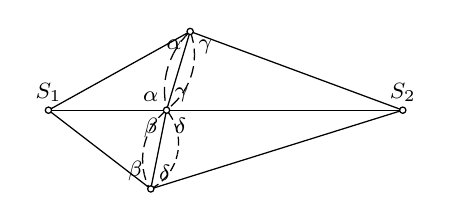
\begin{tikzpicture}
                    % \clip (0,0) rectangle (14.000000,10.000000);
                    {\footnotesize
                    
                    % Drawing segment S_1 S_2
                    \draw [line width=0.016cm] (1.540000,2.500000) -- (2.960000,2.500000);%
                    \draw [line width=0.016cm] (3.040000,2.500000) -- (5.960000,2.500000);%
                    
                    % Marking point S_1 by circle
                    \draw [line width=0.016cm] (1.500000,2.500000) circle (0.040000);%
                    \draw (1.500000,2.500000) node [anchor=south] { $S_1$ };%
                    
                    % Marking point S_2 by circle
                    \draw [line width=0.016cm] (6.000000,2.500000) circle (0.040000);%
                    \draw (6.000000,2.500000) node [anchor=south] { $S_2$ };%
                    
                    % Marking point P by circle
                    \draw [line width=0.016cm] (3.300000,3.500000) circle (0.040000);%
                    
                    % Marking point Q by circle
                    \draw [line width=0.016cm] (2.800000,1.500000) circle (0.040000);%
                    
                    % Marking point A by circle
                    \draw [line width=0.016cm] (3.000000,2.500000) circle (0.040000);%
                    
                    % Drawing segment S_1 P
                    \draw [line width=0.016cm] (1.534966,2.519426) -- (3.265034,3.480574);%
                    
                    % Drawing segment S_1 Q
                    \draw [line width=0.016cm] (1.531705,2.475612) -- (2.768295,1.524388);%
                    
                    % Drawing segment S_2 P
                    \draw [line width=0.016cm] (5.962490,2.513893) -- (3.337510,3.486107);%
                    
                    % Drawing segment S_2 Q
                    \draw [line width=0.016cm] (5.961821,2.488069) -- (2.838179,1.511931);%
                    
                    % Drawing segment P A
                    \draw [line width=0.016cm] (3.288506,3.461687) -- (3.011494,2.538313);%
                    
                    % Drawing segment Q A
                    \draw [line width=0.016cm] (2.807845,1.539223) -- (2.992155,2.460777);%
                    
                    % Drawing arc X P 62.00
                    \draw [line width=0.016cm] (3.271295,3.472142) -- (3.262019,3.462660) arc (136:137:1.025914 and 1.025914) -- (3.238118,3.437048);%
                    \draw [line width=0.016cm] (3.238118,3.437048) -- (3.237597,3.436471) arc (138:142:1.025914 and 1.025914) -- (3.181876,3.369010);%
                    \draw [line width=0.016cm] (3.131692,3.296389) -- (3.129975,3.293652) arc (148:152:1.025914 and 1.025914) -- (3.087936,3.219722);%
                    \draw [line width=0.016cm] (3.087936,3.219722) -- (3.085904,3.215755) arc (153:157:1.025914 and 1.025914) -- (3.050932,3.139578);%
                    \draw [line width=0.016cm] (3.020956,3.056549) -- (3.018913,3.049948) arc (163:167:1.025914 and 1.025914) -- (2.998228,2.971251);%
                    \draw [line width=0.016cm] (2.998228,2.971251) -- (2.996504,2.963300) arc (168:172:1.025914 and 1.025914) -- (2.982916,2.884315);%
                    \draw [line width=0.016cm] (2.975135,2.796384) -- (2.974711,2.785804) arc (178:182:1.025914 and 1.025914) -- (2.974941,2.708110);%
                    \draw [line width=0.016cm] (2.974941,2.708111) -- (2.975492,2.696308) arc (183:187:1.025914 and 1.025914) -- (2.982337,2.620147);%
                    
                    % Drawing arc Y A 80.00
                    \draw [line width=0.016cm] (2.969296,2.474362) -- (2.961818,2.467712) arc (132:133:0.804301 and 0.804301) -- (2.946995,2.454025);%
                    \draw [line width=0.016cm] (2.946995,2.454025) -- (2.941286,2.448566) arc (134:138:0.804301 and 0.804301) -- (2.898198,2.403605);%
                    \draw [line width=0.016cm] (2.853981,2.349124) -- (2.849307,2.342756) arc (144:148:0.804301 and 0.804301) -- (2.814681,2.290996);%
                    \draw [line width=0.016cm] (2.814681,2.290996) -- (2.810580,2.284246) arc (149:153:0.804301 and 0.804301) -- (2.780597,2.229665);%
                    \draw [line width=0.016cm] (2.751987,2.165596) -- (2.749120,2.158236) arc (159:163:0.804301 and 0.804301) -- (2.729071,2.099278);%
                    \draw [line width=0.016cm] (2.729071,2.099278) -- (2.726856,2.091695) arc (164:168:0.804301 and 0.804301) -- (2.712022,2.031214);%
                    \draw [line width=0.016cm] (2.700969,1.961924) -- (2.700105,1.954072) arc (174:178:0.804301 and 0.804301) -- (2.695998,1.891934);%
                    \draw [line width=0.016cm] (2.695998,1.891934) -- (2.695822,1.884037) arc (179:183:0.804301 and 0.804301) -- (2.697146,1.821777);%
                    \draw [line width=0.016cm] (2.704404,1.751988) -- (2.705601,1.744180) arc (189:193:0.804301 and 0.804301) -- (2.717717,1.683096);%
                    \draw [line width=0.016cm] (2.717717,1.683096) -- (2.719590,1.675422) arc (194:198:0.804301 and 0.804301) -- (2.736983,1.615627);%
                    \draw [line width=0.016cm] (2.762057,1.550093) -- (2.765234,1.542861) arc (204:205:0.804301 and 0.804301) -- (2.771841,1.528409);%
                    
                    % Drawing arc Z P -70.00
                    \draw [line width=0.016cm] (3.055524,2.550852) -- (3.060537,2.555176) arc (311:315:0.854400 and 0.854400) -- (3.109987,2.601739);%
                    \draw [line width=0.016cm] (3.109987,2.601739) -- (3.114604,2.606483) arc (316:320:0.854400 and 0.854400) -- (3.159807,2.657180);%
                    \draw [line width=0.016cm] (3.204607,2.716751) -- (3.208330,2.722225) arc (326:330:0.854400 and 0.854400) -- (3.244043,2.780001);%
                    \draw [line width=0.016cm] (3.244043,2.780001) -- (3.247275,2.785778) arc (331:335:0.854400 and 0.854400) -- (3.277817,2.846446);%
                    \draw [line width=0.016cm] (3.305672,2.915583) -- (3.307851,2.921834) arc (341:345:0.854400 and 0.854400) -- (3.327395,2.986884);%
                    \draw [line width=0.016cm] (3.327395,2.986884) -- (3.329021,2.993302) arc (346:350:0.854400 and 0.854400) -- (3.342820,3.059807);%
                    \draw [line width=0.016cm] (3.351832,3.133797) -- (3.352319,3.140400) arc (356:360:0.854400 and 0.854400) --(3.354400,3.200000) arc (0:0:0.854400 and 0.854400) -- (3.354360,3.208292);%
                    \draw [line width=0.016cm] (3.354360,3.208292) -- (3.354270,3.214911) arc (1:5:0.854400 and 0.854400) -- (3.350386,3.282723);%
                    \draw [line width=0.016cm] (3.339941,3.356524) -- (3.338703,3.363027) arc (11:15:0.854400 and 0.854400) -- (3.323102,3.429134);%
                    \draw [line width=0.016cm] (3.323102,3.429134) -- (3.321302,3.435505) arc (16:17:0.854400 and 0.854400) -- (3.313164,3.462228);%
                    
                    % Drawing arc W Q 105.00
                    \draw [line width=0.016cm] (2.834949,1.519456) -- (2.836316,1.520276) arc (301:302:0.652993 and 0.652993) -- (2.849409,1.528354);%
                    \draw [line width=0.016cm] (2.849409,1.528354) -- (2.855645,1.532354) arc (303:307:0.652993 and 0.652993) -- (2.896158,1.560906);%
                    \draw [line width=0.016cm] (2.939893,1.597409) -- (2.945340,1.602431) arc (313:317:0.652993 and 0.652993) -- (2.980279,1.637584);%
                    \draw [line width=0.016cm] (2.980279,1.637584) -- (2.985268,1.643062) arc (318:322:0.652993 and 0.652993) -- (3.017011,1.681127);%
                    \draw [line width=0.016cm] (3.049808,1.727705) -- (3.053769,1.733966) arc (328:332:0.652993 and 0.652993) -- (3.078420,1.776965);%
                    \draw [line width=0.016cm] (3.078420,1.776965) -- (3.081821,1.783547) arc (333:337:0.652993 and 0.652993) -- (3.102630,1.828530);%
                    \draw [line width=0.016cm] (3.122254,1.882010) -- (3.124460,1.889083) arc (343:347:0.652993 and 0.652993) -- (3.137142,1.936996);%
                    \draw [line width=0.016cm] (3.137142,1.936996) -- (3.138724,1.944235) arc (348:352:0.652993 and 0.652993) -- (3.147181,1.993071);%
                    \draw [line width=0.016cm] (3.152295,2.049807) -- (3.152595,2.057211) arc (358:360:0.652993 and 0.652993) --(3.152993,2.080000) arc (0:2:0.652993 and 0.652993) -- (3.152444,2.106774);%
                    \draw [line width=0.016cm] (3.152444,2.106774) -- (3.152098,2.114175) arc (3:7:0.652993 and 0.652993) -- (3.147628,2.163536);%
                    \draw [line width=0.016cm] (3.137883,2.219663) -- (3.136257,2.226891) arc (13:17:0.652993 and 0.652993) -- (3.123283,2.274726);%
                    \draw [line width=0.016cm] (3.123283,2.274726) -- (3.121033,2.281786) arc (18:22:0.652993 and 0.652993) -- (3.103940,2.328308);%
                    \draw [line width=0.016cm] (3.080000,2.380000) -- (3.076559,2.386562) arc (28:32:0.652993 and 0.652993) -- (3.051646,2.429409);%
                    \draw [line width=0.016cm] (3.051646,2.429409) -- (3.047646,2.435646) arc (33:36:0.652993 and 0.652993) -- (3.024778,2.468598);%
                    
                    % Marking point \alpha
                    \draw (3.000000,2.500000) node [anchor=south east] { $\alpha$ };%
                    
                    % Marking point \beta
                    \draw (3.000000,2.500000) node [anchor=north east] { $\beta$ };%
                    
                    % Marking point \gamma
                    \draw (3.000000,2.500000) node [anchor=south west] { $\gamma$ };%
                    
                    % Marking point \delta
                    \draw (3.000000,2.500000) node [anchor=north west] { $\delta$ };%
                    
                    % Marking point \alpha
                    \draw (3.300000,3.500000) node [anchor=north east] { $\alpha$ };%
                    
                    % Marking point \beta
                    \draw (2.800000,1.500000) node [anchor=south east] { $\beta$ };%
                    
                    % Marking point \gamma
                    \draw (3.300000,3.500000) node [anchor=north west] { $\gamma$ };%
                    
                    % Marking point \delta
                    \draw (2.800000,1.500000) node [anchor=south west] { $\delta$ };%
                    }
                \end{tikzpicture}                    
                \\ Ker je vsota poljubnih dve kotov v trikotniku manjša od $\pi$, je: $\alpha <\frac{\pi}{2}, \beta<\frac{\pi}{2}, \gamma<\frac{\pi}{2}, \delta<\frac{\pi}{2}$. Potem je $\alpha+\beta+\gamma+\delta<2\pi$, kar pa je protislovje. (Dokaz je podoben, če sta središči na isti strani.)
            \end{dokaz}

        \begin{trditev}[III.11, III.12]
            Če sta krožnici tangentni (se sekata natanko v eni točki), potem so dotikališče in središči krožnic kolinearne točke.
        \end{trditev}

            \begin{dokaz}
                \\ \begin{tikzpicture}
                    % \clip (0,0) rectangle (14.000000,10.000000);
                    {\footnotesize
                    
                    % Drawing circle S_1 D
                    \draw [line width=0.016cm] (4.999680,3.539999) -- (4.999619,3.543631) arc (1:1:2.500000 and 2.500000) -- (4.998477,3.587249);%
                    \draw [line width=0.016cm] (4.998477,3.587249) -- (4.998477,3.587249) arc (2:3:2.500000 and 2.500000) -- (4.993910,3.674391);%
                    \draw [line width=0.016cm] (4.986305,3.761321) -- (4.986305,3.761321) arc (6:6:2.500000 and 2.500000) -- (4.986185,3.762462);%
                    \draw [line width=0.016cm] (4.977696,3.833204) -- (4.975670,3.847933) arc (8:8:2.500000 and 2.500000);%
                    \draw [line width=0.016cm] (4.975670,3.847933) -- (4.975670,3.847933) arc (8:9:2.500000 and 2.500000) -- (4.962019,3.934120);%
                    \draw [line width=0.016cm] (4.945369,4.019779) -- (4.945369,4.019779) arc (12:13:2.500000 and 2.500000) -- (4.925739,4.104805);%
                    \draw [line width=0.016cm] (4.925739,4.104805) arc (14:16:2.500000 and 2.500000);%
                    \draw [line width=0.016cm] (4.877641,4.272542) arc (18:20:2.500000 and 2.500000);%
                    \draw [line width=0.016cm] (4.849232,4.355050) -- (4.849232,4.355050) arc (20:21:2.500000 and 2.500000) -- (4.817960,4.436516);%
                    \draw [line width=0.016cm] (4.783864,4.516842) -- (4.783864,4.516842) arc (24:25:2.500000 and 2.500000) -- (4.746985,4.595928);%
                    \draw [line width=0.016cm] (4.746985,4.595928) -- (4.746985,4.595928) arc (26:27:2.500000 and 2.500000) -- (4.707369,4.673679);%
                    \draw [line width=0.016cm] (4.665064,4.750000) -- (4.665064,4.750000) arc (30:31:2.500000 and 2.500000) -- (4.620120,4.824798);%
                    \draw [line width=0.016cm] (4.620120,4.824798) -- (4.620120,4.824798) arc (32:33:2.500000 and 2.500000) -- (4.572594,4.897982);%
                    \draw [line width=0.016cm] (4.522543,4.969463) -- (4.522543,4.969463) arc (36:37:2.500000 and 2.500000) -- (4.470027,5.039154);%
                    \draw [line width=0.016cm] (4.470027,5.039154) -- (4.470027,5.039154) arc (38:39:2.500000 and 2.500000) -- (4.415111,5.106969);%
                    \draw [line width=0.016cm] (4.357862,5.172826) -- (4.357862,5.172826) arc (42:43:2.500000 and 2.500000) -- (4.298350,5.236646);%
                    \draw [line width=0.016cm] (4.298350,5.236646) -- (4.298350,5.236646) arc (44:45:2.500000 and 2.500000) -- (4.236646,5.298349);%
                    \draw [line width=0.016cm] (4.172827,5.357862) -- (4.172827,5.357862) arc (48:49:2.500000 and 2.500000) -- (4.106969,5.415111);%
                    \draw [line width=0.016cm] (4.106969,5.415111) -- (4.106969,5.415111) arc (50:51:2.500000 and 2.500000) -- (4.039154,5.470027);%
                    \draw [line width=0.016cm] (3.969463,5.522542) -- (3.969463,5.522542) arc (54:55:2.500000 and 2.500000) -- (3.897982,5.572594);%
                    \draw [line width=0.016cm] (3.897982,5.572594) -- (3.897982,5.572594) arc (56:57:2.500000 and 2.500000) -- (3.824798,5.620120);%
                    \draw [line width=0.016cm] (3.750000,5.665063) -- (3.750000,5.665063) arc (60:61:2.500000 and 2.500000) -- (3.673679,5.707369);%
                    \draw [line width=0.016cm] (3.673679,5.707369) -- (3.673679,5.707369) arc (62:63:2.500000 and 2.500000) -- (3.595928,5.746985);%
                    \draw [line width=0.016cm] (3.516842,5.783864) -- (3.516842,5.783864) arc (66:67:2.500000 and 2.500000) -- (3.436517,5.817960);%
                    \draw [line width=0.016cm] (3.436517,5.817960) -- (3.436517,5.817960) arc (68:69:2.500000 and 2.500000) -- (3.355050,5.849232);%
                    \draw [line width=0.016cm] (3.272543,5.877641) -- (3.272543,5.877641) arc (72:73:2.500000 and 2.500000) -- (3.189094,5.903154);%
                    \draw [line width=0.016cm] (3.189094,5.903154) -- (3.189094,5.903154) arc (74:75:2.500000 and 2.500000) -- (3.104805,5.925739);%
                    \draw [line width=0.016cm] (3.019779,5.945369) -- (3.019779,5.945369) arc (78:79:2.500000 and 2.500000) -- (2.934121,5.962019);%
                    \draw [line width=0.016cm] (2.934121,5.962019) -- (2.934121,5.962019) arc (80:81:2.500000 and 2.500000) -- (2.847933,5.975670);%
                    \draw [line width=0.016cm] (2.761321,5.986305) -- (2.761321,5.986305) arc (84:85:2.500000 and 2.500000) -- (2.674391,5.993910);%
                    \draw [line width=0.016cm] (2.674391,5.993910) -- (2.674391,5.993910) arc (86:87:2.500000 and 2.500000) -- (2.587249,5.998477);%
                    \draw [line width=0.016cm] (2.500000,6.000000) -- (2.500000,6.000000) arc (90:91:2.500000 and 2.500000) -- (2.412751,5.998477);%
                    \draw [line width=0.016cm] (2.412751,5.998477) -- (2.412751,5.998477) arc (92:93:2.500000 and 2.500000) -- (2.325609,5.993910);%
                    \draw [line width=0.016cm] (2.238679,5.986305) -- (2.238679,5.986305) arc (96:97:2.500000 and 2.500000) -- (2.152067,5.975670);%
                    \draw [line width=0.016cm] (2.152067,5.975670) -- (2.152067,5.975670) arc (98:99:2.500000 and 2.500000) -- (2.065880,5.962019);%
                    \draw [line width=0.016cm] (1.980221,5.945369) -- (1.980221,5.945369) arc (102:103:2.500000 and 2.500000) -- (1.895195,5.925739);%
                    \draw [line width=0.016cm] (1.895195,5.925739) -- (1.895195,5.925739) arc (104:105:2.500000 and 2.500000) -- (1.810907,5.903154);%
                    \draw [line width=0.016cm] (1.727458,5.877641) -- (1.727458,5.877641) arc (108:109:2.500000 and 2.500000) -- (1.644950,5.849232);%
                    \draw [line width=0.016cm] (1.644950,5.849232) -- (1.644950,5.849232) arc (110:111:2.500000 and 2.500000) -- (1.563484,5.817960);%
                    \draw [line width=0.016cm] (1.483159,5.783864) arc (114:116:2.500000 and 2.500000);%
                    \draw [line width=0.016cm] (1.404072,5.746985) arc (116:118:2.500000 and 2.500000);%
                    \draw [line width=0.016cm] (1.250000,5.665064) -- (1.250000,5.665064) arc (120:121:2.500000 and 2.500000) -- (1.175202,5.620120);%
                    \draw [line width=0.016cm] (1.175202,5.620120) arc (122:124:2.500000 and 2.500000);%
                    \draw [line width=0.016cm] (1.030537,5.522543) arc (126:126:2.500000 and 2.500000) -- (1.000000,5.500000);%
                    \draw [line width=0.016cm] (1.030536,1.477458) -- (1.030536,1.477458) arc (234:235:2.500000 and 2.500000) -- (1.102017,1.427407);%
                    \draw [line width=0.016cm] (1.102017,1.427407) -- (1.102017,1.427406) arc (236:237:2.500000 and 2.500000) -- (1.175201,1.379880);%
                    \draw [line width=0.016cm] (1.249999,1.334937) -- (1.250000,1.334937) arc (240:241:2.500000 and 2.500000) -- (1.326320,1.292632);%
                    \draw [line width=0.016cm] (1.326320,1.292632) -- (1.326321,1.292631) arc (242:243:2.500000 and 2.500000) -- (1.404071,1.253015);%
                    \draw [line width=0.016cm] (1.483157,1.216137) -- (1.483158,1.216137) arc (246:247:2.500000 and 2.500000) -- (1.563482,1.182041);%
                    \draw [line width=0.016cm] (1.563482,1.182041) -- (1.563483,1.182041) arc (248:249:2.500000 and 2.500000) -- (1.644948,1.150769);%
                    \draw [line width=0.016cm] (1.727456,1.122359) -- (1.727457,1.122359) arc (252:253:2.500000 and 2.500000) -- (1.810905,1.096846);%
                    \draw [line width=0.016cm] (1.810905,1.096846) -- (1.810906,1.096846) arc (254:255:2.500000 and 2.500000) -- (1.895194,1.074261);%
                    \draw [line width=0.016cm] (1.980219,1.054631) -- (1.980220,1.054631) arc (258:259:2.500000 and 2.500000) -- (2.065878,1.037981);%
                    \draw [line width=0.016cm] (2.065878,1.037981) -- (2.065879,1.037981) arc (260:261:2.500000 and 2.500000) -- (2.152066,1.024330);%
                    \draw [line width=0.016cm] (2.238678,1.013695) -- (2.238678,1.013695) arc (264:265:2.500000 and 2.500000) -- (2.325607,1.006090);%
                    \draw [line width=0.016cm] (2.325607,1.006090) -- (2.325608,1.006090) arc (266:267:2.500000 and 2.500000) -- (2.412750,1.001523);%
                    \draw [line width=0.016cm] (2.499999,1.000000) -- (2.499999,1.000000) arc (270:271:2.500000 and 2.500000) -- (2.587247,1.001523);%
                    \draw [line width=0.016cm] (2.587247,1.001523) -- (2.587248,1.001523) arc (272:273:2.500000 and 2.500000) -- (2.674390,1.006090);%
                    \draw [line width=0.016cm] (2.761320,1.013695) -- (2.761321,1.013695) arc (276:277:2.500000 and 2.500000) -- (2.847931,1.024330);%
                    \draw [line width=0.016cm] (2.847931,1.024330) -- (2.847932,1.024330) arc (278:279:2.500000 and 2.500000) -- (2.934119,1.037980);%
                    \draw [line width=0.016cm] (3.019778,1.054631) -- (3.019779,1.054631) arc (282:283:2.500000 and 2.500000) -- (3.104803,1.074260);%
                    \draw [line width=0.016cm] (3.104803,1.074260) -- (3.104804,1.074261) arc (284:285:2.500000 and 2.500000) -- (3.189092,1.096845);%
                    \draw [line width=0.016cm] (3.272541,1.122358) -- (3.272542,1.122359) arc (288:289:2.500000 and 2.500000) -- (3.355049,1.150768);%
                    \draw [line width=0.016cm] (3.355049,1.150768) -- (3.355050,1.150768) arc (290:291:2.500000 and 2.500000) -- (3.436515,1.182040);%
                    \draw [line width=0.016cm] (3.516840,1.216136) -- (3.516841,1.216136) arc (294:295:2.500000 and 2.500000) -- (3.595927,1.253014);%
                    \draw [line width=0.016cm] (3.595927,1.253014) -- (3.595927,1.253015) arc (296:297:2.500000 and 2.500000) -- (3.673678,1.292630);%
                    \draw [line width=0.016cm] (3.749999,1.334936) -- (3.749999,1.334936) arc (300:301:2.500000 and 2.500000) -- (3.824797,1.379879);%
                    \draw [line width=0.016cm] (3.824797,1.379879) -- (3.824798,1.379879) arc (302:303:2.500000 and 2.500000) -- (3.897981,1.427405);%
                    \draw [line width=0.016cm] (3.969462,1.477457) -- (3.969463,1.477457) arc (306:307:2.500000 and 2.500000) -- (4.039153,1.529972);%
                    \draw [line width=0.016cm] (4.039153,1.529972) -- (4.039153,1.529973) arc (308:309:2.500000 and 2.500000) -- (4.106968,1.584888);%
                    \draw [line width=0.016cm] (4.172825,1.642137) -- (4.172826,1.642137) arc (312:313:2.500000 and 2.500000) -- (4.236645,1.701650);%
                    \draw [line width=0.016cm] (4.236645,1.701650) -- (4.236645,1.701650) arc (314:315:2.500000 and 2.500000) -- (4.298348,1.763353);%
                    \draw [line width=0.016cm] (4.357861,1.827172) -- (4.357862,1.827173) arc (318:319:2.500000 and 2.500000) -- (4.415110,1.893030);%
                    \draw [line width=0.016cm] (4.415110,1.893030) -- (4.415111,1.893030) arc (320:321:2.500000 and 2.500000) -- (4.470026,1.960845);%
                    \draw [line width=0.016cm] (4.522542,2.030536) -- (4.522542,2.030536) arc (324:325:2.500000 and 2.500000) -- (4.572593,2.102017);%
                    \draw [line width=0.016cm] (4.572593,2.102017) -- (4.572594,2.102017) arc (326:327:2.500000 and 2.500000) -- (4.620119,2.175201);%
                    \draw [line width=0.016cm] (4.665063,2.249999) -- (4.665063,2.249999) arc (330:331:2.500000 and 2.500000) -- (4.707368,2.326320);%
                    \draw [line width=0.016cm] (4.707368,2.326320) -- (4.707369,2.326320) arc (332:333:2.500000 and 2.500000) -- (4.746984,2.404071);%
                    \draw [line width=0.016cm] (4.783863,2.483157) -- (4.783863,2.483158) arc (336:337:2.500000 and 2.500000) -- (4.817959,2.563482);%
                    \draw [line width=0.016cm] (4.817959,2.563482) -- (4.817959,2.563483) arc (338:339:2.500000 and 2.500000) -- (4.849231,2.644948);%
                    \draw [line width=0.016cm] (4.877641,2.727456) -- (4.877641,2.727457) arc (342:343:2.500000 and 2.500000) -- (4.903154,2.810905);%
                    \draw [line width=0.016cm] (4.903154,2.810905) -- (4.903154,2.810906) arc (344:345:2.500000 and 2.500000) -- (4.925739,2.895194);%
                    \draw [line width=0.016cm] (4.945369,2.980219) -- (4.945369,2.980220) arc (348:349:2.500000 and 2.500000) -- (4.962019,3.065878);%
                    \draw [line width=0.016cm] (4.962019,3.065878) -- (4.962019,3.065879) arc (350:351:2.500000 and 2.500000) -- (4.975670,3.152066);%
                    \draw [line width=0.016cm] (4.986305,3.238677) -- (4.986305,3.238678) arc (354:355:2.500000 and 2.500000) -- (4.993910,3.325607);%
                    \draw [line width=0.016cm] (4.993910,3.325607) -- (4.993910,3.325608) arc (356:357:2.500000 and 2.500000) -- (4.998477,3.412750);%
                    
                    % Drawing circle S_2 D
                    \draw [line width=0.016cm] (5.000400,3.460003) -- (5.001218,3.430201) arc (182:182:2.000000 and 2.000000) -- (5.001904,3.412762);%
                    \draw [line width=0.016cm] (5.001904,3.412762) -- (5.002741,3.395328) arc (183:184:2.000000 and 2.000000) -- (5.007611,3.325689);%
                    \draw [line width=0.016cm] (5.017110,3.238948) -- (5.019464,3.221654) arc (188:189:2.000000 and 2.000000) -- (5.030384,3.152704);%
                    \draw [line width=0.016cm] (5.030384,3.152704) -- (5.030384,3.152704) arc (190:192:2.000000 and 2.000000) -- (5.047408,3.067121);%
                    \draw [line width=0.016cm] (5.068148,2.982363) -- (5.068148,2.982362) arc (195:197:2.000000 and 2.000000) -- (5.092566,2.898589);%
                    \draw [line width=0.016cm] (5.092566,2.898589) -- (5.097887,2.881966) arc (198:199:2.000000 and 2.000000) -- (5.120615,2.815960);%
                    \draw [line width=0.016cm] (5.152241,2.734634) -- (5.158990,2.718538) arc (203:204:2.000000 and 2.000000) -- (5.187384,2.654764);%
                    \draw [line width=0.016cm] (5.187384,2.654764) -- (5.187384,2.654764) arc (205:207:2.000000 and 2.000000) -- (5.225978,2.576503);%
                    \draw [line width=0.016cm] (5.267949,2.500001) -- (5.267949,2.500000) arc (210:212:2.000000 and 2.000000) -- (5.313217,2.425401);%
                    \draw [line width=0.016cm] (5.313217,2.425401) -- (5.322659,2.410722) arc (213:214:2.000000 and 2.000000) -- (5.361696,2.352848);%
                    \draw [line width=0.016cm] (5.413293,2.282478) -- (5.423978,2.268677) arc (218:219:2.000000 and 2.000000) -- (5.467911,2.214425);%
                    \draw [line width=0.016cm] (5.467911,2.214425) -- (5.467911,2.214425) arc (220:222:2.000000 and 2.000000) -- (5.525445,2.148820);%
                    \draw [line width=0.016cm] (5.585786,2.085787) -- (5.585786,2.085787) arc (225:227:2.000000 and 2.000000) -- (5.648819,2.025446);%
                    \draw [line width=0.016cm] (5.648819,2.025446) -- (5.661738,2.013711) arc (228:229:2.000000 and 2.000000) -- (5.714424,1.967912);%
                    \draw [line width=0.016cm] (5.782477,1.913294) -- (5.796370,1.902729) arc (233:234:2.000000 and 2.000000) -- (5.852847,1.861696);%
                    \draw [line width=0.016cm] (5.852847,1.861696) -- (5.852847,1.861696) arc (235:237:2.000000 and 2.000000) -- (5.925400,1.813217);%
                    \draw [line width=0.016cm] (5.999999,1.767950) -- (6.000000,1.767949) arc (240:242:2.000000 and 2.000000) -- (6.076502,1.725979);%
                    \draw [line width=0.016cm] (6.076502,1.725979) -- (6.092019,1.717987) arc (243:244:2.000000 and 2.000000) -- (6.154763,1.687385);%
                    \draw [line width=0.016cm] (6.234632,1.652241) -- (6.250786,1.645632) arc (248:249:2.000000 and 2.000000) -- (6.315959,1.620615);%
                    \draw [line width=0.016cm] (6.315959,1.620615) -- (6.315959,1.620615) arc (250:252:2.000000 and 2.000000) -- (6.398588,1.592566);%
                    \draw [line width=0.016cm] (6.482361,1.568149) -- (6.482361,1.568148) arc (255:257:2.000000 and 2.000000) -- (6.567120,1.547408);%
                    \draw [line width=0.016cm] (6.567120,1.547408) -- (6.584176,1.543705) arc (258:259:2.000000 and 2.000000) -- (6.652703,1.530385);%
                    \draw [line width=0.016cm] (6.738947,1.517110) -- (6.756261,1.514908) arc (263:264:2.000000 and 2.000000) -- (6.825688,1.507611);%
                    \draw [line width=0.016cm] (6.825688,1.507611) -- (6.825688,1.507611) arc (265:267:2.000000 and 2.000000) -- (6.912760,1.501904);%
                    \draw [line width=0.016cm] (6.999999,1.500000) -- (7.000000,1.500000) arc (270:272:2.000000 and 2.000000) -- (7.087238,1.501904);%
                    \draw [line width=0.016cm] (7.087238,1.501904) -- (7.104671,1.502741) arc (273:274:2.000000 and 2.000000) -- (7.174311,1.507611);%
                    \draw [line width=0.016cm] (7.261052,1.517110) -- (7.278346,1.519464) arc (278:279:2.000000 and 2.000000) -- (7.347296,1.530384);%
                    \draw [line width=0.016cm] (7.347296,1.530384) -- (7.347296,1.530384) arc (280:282:2.000000 and 2.000000) -- (7.432878,1.547408);%
                    \draw [line width=0.016cm] (7.517637,1.568148) -- (7.517638,1.568148) arc (285:287:2.000000 and 2.000000) -- (7.601411,1.592566);%
                    \draw [line width=0.016cm] (7.601411,1.592566) -- (7.618034,1.597887) arc (288:289:2.000000 and 2.000000) -- (7.684040,1.620614);%
                    \draw [line width=0.016cm] (7.765366,1.652241) -- (7.781462,1.658990) arc (293:294:2.000000 and 2.000000) -- (7.845236,1.687384);%
                    \draw [line width=0.016cm] (7.845236,1.687384) -- (7.845236,1.687384) arc (295:297:2.000000 and 2.000000) -- (7.923497,1.725978);%
                    \draw [line width=0.016cm] (7.999999,1.767949) arc (299:299:2.000000 and 2.000000) -- (7.999999,1.767949);%
                    \draw [line width=0.016cm] (8.000000,5.232051) arc (60:62:2.000000 and 2.000000) -- (7.923498,5.274021);%
                    \draw [line width=0.016cm] (7.923498,5.274021) -- (7.907981,5.282013) arc (63:64:2.000000 and 2.000000) -- (7.845237,5.312615);%
                    \draw [line width=0.016cm] (7.765367,5.347759) -- (7.749213,5.354368) arc (68:69:2.000000 and 2.000000) -- (7.684041,5.379385);%
                    \draw [line width=0.016cm] (7.684041,5.379385) -- (7.684040,5.379385) arc (70:72:2.000000 and 2.000000) -- (7.601412,5.407434);%
                    \draw [line width=0.016cm] (7.517639,5.431852) -- (7.517638,5.431852) arc (75:77:2.000000 and 2.000000) -- (7.432880,5.452592);%
                    \draw [line width=0.016cm] (7.432880,5.452592) -- (7.415824,5.456295) arc (78:79:2.000000 and 2.000000) -- (7.347297,5.469615);%
                    \draw [line width=0.016cm] (7.261053,5.482890) -- (7.243739,5.485092) arc (83:84:2.000000 and 2.000000) -- (7.174312,5.492389);%
                    \draw [line width=0.016cm] (7.174312,5.492389) -- (7.174312,5.492389) arc (85:87:2.000000 and 2.000000) -- (7.087239,5.498096);%
                    \draw [line width=0.016cm] (7.000000,5.500000) -- (7.000000,5.500000) arc (90:92:2.000000 and 2.000000) -- (6.912762,5.498096);%
                    \draw [line width=0.016cm] (6.912762,5.498096) -- (6.895328,5.497259) arc (93:94:2.000000 and 2.000000) -- (6.825689,5.492389);%
                    \draw [line width=0.016cm] (6.738948,5.482890) -- (6.721654,5.480536) arc (98:99:2.000000 and 2.000000) -- (6.652704,5.469616);%
                    \draw [line width=0.016cm] (6.652704,5.469616) -- (6.652704,5.469616) arc (100:102:2.000000 and 2.000000) -- (6.567121,5.452592);%
                    \draw [line width=0.016cm] (6.482362,5.431852) -- (6.482362,5.431852) arc (105:107:2.000000 and 2.000000) -- (6.398589,5.407434);%
                    \draw [line width=0.016cm] (6.398589,5.407434) -- (6.381966,5.402113) arc (108:109:2.000000 and 2.000000) -- (6.315960,5.379385);%
                    \draw [line width=0.016cm] (6.234634,5.347759) -- (6.218538,5.341010) arc (113:114:2.000000 and 2.000000) -- (6.154764,5.312616);%
                    \draw [line width=0.016cm] (6.154764,5.312616) -- (6.154764,5.312616) arc (115:117:2.000000 and 2.000000) -- (6.076503,5.274022);%
                    \draw [line width=0.016cm] (6.000000,5.232051) -- (6.000000,5.232051) arc (120:122:2.000000 and 2.000000) -- (5.925401,5.186783);%
                    \draw [line width=0.016cm] (5.925401,5.186783) -- (5.910722,5.177341) arc (123:124:2.000000 and 2.000000) -- (5.852848,5.138304);%
                    \draw [line width=0.016cm] (5.782478,5.086707) -- (5.768677,5.076022) arc (128:129:2.000000 and 2.000000) -- (5.714425,5.032089);%
                    \draw [line width=0.016cm] (5.714425,5.032089) -- (5.714425,5.032089) arc (130:132:2.000000 and 2.000000) -- (5.648820,4.974555);%
                    \draw [line width=0.016cm] (5.585787,4.914214) -- (5.585787,4.914214) arc (135:137:2.000000 and 2.000000) -- (5.525446,4.851181);%
                    \draw [line width=0.016cm] (5.525446,4.851181) -- (5.513711,4.838261) arc (138:139:2.000000 and 2.000000) -- (5.467911,4.785576);%
                    \draw [line width=0.016cm] (5.413294,4.717523) -- (5.402729,4.703630) arc (143:144:2.000000 and 2.000000) -- (5.361696,4.647153);%
                    \draw [line width=0.016cm] (5.361696,4.647153) -- (5.361696,4.647153) arc (145:147:2.000000 and 2.000000) -- (5.313217,4.574600);%
                    \draw [line width=0.016cm] (5.267949,4.500000) -- (5.267949,4.500000) arc (150:152:2.000000 and 2.000000) -- (5.225979,4.423498);%
                    \draw [line width=0.016cm] (5.225979,4.423498) -- (5.217987,4.407981) arc (153:154:2.000000 and 2.000000) -- (5.187385,4.345237);%
                    \draw [line width=0.016cm] (5.152241,4.265367) -- (5.145632,4.249213) arc (158:159:2.000000 and 2.000000) -- (5.120615,4.184041);%
                    \draw [line width=0.016cm] (5.120615,4.184041) -- (5.120615,4.184041) arc (160:162:2.000000 and 2.000000) -- (5.092566,4.101412);%
                    \draw [line width=0.016cm] (5.068148,4.017639) -- (5.068148,4.017638) arc (165:167:2.000000 and 2.000000) -- (5.047408,3.932880);%
                    \draw [line width=0.016cm] (5.047408,3.932880) -- (5.043705,3.915824) arc (168:169:2.000000 and 2.000000) -- (5.030385,3.847297);%
                    \draw [line width=0.016cm] (5.017110,3.761053) -- (5.014908,3.743739) arc (173:174:2.000000 and 2.000000) -- (5.007611,3.674312);%
                    \draw [line width=0.016cm] (5.007611,3.674312) -- (5.007611,3.674312) arc (175:177:2.000000 and 2.000000) -- (5.001904,3.587239);%
                    
                    % Marking point S_1 by circle
                    \draw [line width=0.016cm] (2.500000,3.500000) circle (0.040000);%
                    \draw (2.500000,3.500000) node [anchor=south] { $S_1$ };%
                    
                    % Marking point S_2 by circle
                    \draw [line width=0.016cm] (7.000000,3.500000) circle (0.040000);%
                    \draw (7.000000,3.500000) node [anchor=south] { $S_2$ };%
                    
                    % Marking point T by circle
                    \draw [line width=0.016cm] (5.000000,3.800000) circle (0.040000);%
                    \draw (4.970000,3.770000) node [anchor=south west] { $T$ };%
                    
                    % Marking point D by circle
                    \draw [line width=0.016cm] (5.000000,3.500000) circle (0.040000);%
                    \draw (5.030000,3.530000) node [anchor=north east] { $D$ };%
                    
                    % Drawing segment S_1 S_2
                    \draw [line width=0.016cm] (2.540000,3.500000) -- (4.960000,3.500000);%
                    \draw [line width=0.016cm] (5.040000,3.500000) -- (6.960000,3.500000);%
                    
                    % Drawing segment S_1 T
                    \draw [line width=0.016cm] (2.539715,3.504766) -- (4.960285,3.795234);%
                    
                    % Drawing segment S_2 T
                    \draw [line width=0.016cm] (6.960443,3.505934) -- (5.039557,3.794066);%
                    
                    % Marking point r_1
                    \draw (3.750000,3.500000) node [anchor=north] { $r_1$ };%
                    
                    % Marking point r_2
                    \draw (6.000000,3.500000) node [anchor=north] { $r_2$ };%
                    
                    % Marking point r_1
                    \draw (3.750000,3.650000) node [anchor=south] { $r_1$ };%
                    
                    % Marking point r_2
                    \draw (6.000000,3.650000) node [anchor=south] { $r_2$ };%
                    }
                    \end{tikzpicture}                    
                \\ (v nasprotju s trikotniško neenakostjo)
            \end{dokaz}

        \begin{trditev}[III.20 -- središčni in obodni koti]
            Naj bo dana krožnica  $K$ in točki $A$ in $B$ ($A\neq B$) na krožnici $K$ ter naj bo $l\in K$ lok s krajiščema $A$ in $B$.\\
            Potem je središčni kot nad lokom $l$ enak 2-kratniku obodnega kota nad tem lokom. Tj.\ za poljuben $T\in K\backslash l$ je: $|\angle ASB|=2|\angle ATB|$.
        \end{trditev}

            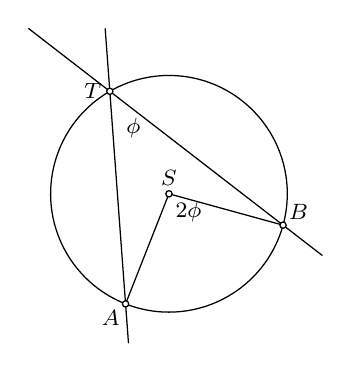
\begin{tikzpicture}
                % \clip (0,0) rectangle (14.000000,10.000000);
                {\footnotesize
                
                % Marking point T by circle
                \draw [line width=0.016cm] (2.800000,4.200000) circle (0.040000);%
                \draw (2.800000,4.200000) node [anchor=east] { $T$ };%
                
                % Marking point A by circle
                \draw [line width=0.016cm] (3.000000,1.500000) circle (0.040000);%
                \draw (3.030000,1.530000) node [anchor=north east] { $A$ };%
                
                % Marking point B by circle
                \draw [line width=0.016cm] (5.000000,2.500000) circle (0.040000);%
                \draw (4.970000,2.470000) node [anchor=south west] { $B$ };%
                
                % Drawing circle S A
                \draw [line width=0.016cm] (3.037407,1.485834) -- (3.061620,1.477264) arc (251:343:1.502826 and 1.502826) -- (4.988888,2.461574);%
                \draw [line width=0.016cm] (5.010085,2.538707) -- (5.015201,2.560152) arc (347:360:1.502826 and 1.502826) --(5.053719,2.898214) arc (0:118:1.502826 and 1.502826) -- (2.834912,4.219523);%
                \draw [line width=0.016cm] (2.765620,4.179554) -- (2.754517,4.172683) arc (122:246:1.502826 and 1.502826) -- (2.962983,1.515157);%
                
                % Drawing segment S B
                \draw [line width=0.016cm] (3.589463,2.887615) -- (4.961430,2.510599);%
                
                % Drawing segment S A
                \draw [line width=0.016cm] (3.536230,2.860999) -- (3.014663,1.537216);%
                
                % Drawing line T A
                \draw [line width=0.016cm] (3.037037,1.000000) -- (3.002955,1.460109);%
                \draw [line width=0.016cm] (2.997045,1.539891) -- (2.802955,4.160109);%
                \draw [line width=0.016cm] (2.797045,4.239891) -- (2.740741,5.000000);%
                
                % Drawing line T B
                \draw [line width=0.016cm] (1.764706,5.000000) -- (2.768349,4.224458);%
                \draw [line width=0.016cm] (2.831651,4.175542) -- (4.968349,2.524458);%
                \draw [line width=0.016cm] (5.031651,2.475542) -- (5.500000,2.113636);%
                
                % Marking point S by circle
                \draw [line width=0.016cm] (3.550893,2.898214) circle (0.040000);%
                \draw (3.550893,2.898214) node [anchor=south] { $S$ };%
                
                % Marking point 2\phi
                \draw (3.800000,2.900000) node [anchor=north] { $2\phi$ };%
                
                % Marking point \phi
                \draw (3.100000,3.500000) node [anchor=south] { $\phi$ };%
                }
            \end{tikzpicture}

            \begin{dokaz}
                \\ Obravnavamo primere glede na lego točk $S$ in $T$. Upoštevamo velikosti zunanjega kota v trikotniku glede na velikosti nasprotnih notranjih kotov.\\
                (1) 
                \\ 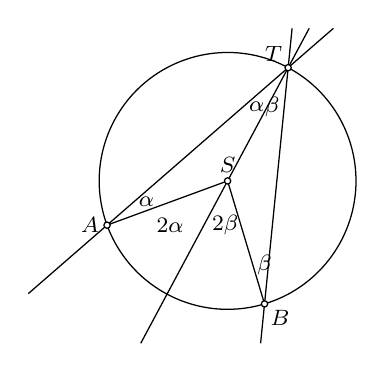
\begin{tikzpicture}
                    % \clip (0,0) rectangle (14.000000,10.000000);
                    {\footnotesize
                    
                    % Marking point T by circle
                    \draw [line width=0.016cm] (4.300000,4.500000) circle (0.040000);%
                    \draw (4.330000,4.470000) node [anchor=south east] { $T$ };%
                    
                    % Marking point A by circle
                    \draw [line width=0.016cm] (2.000000,2.500000) circle (0.040000);%
                    \draw (2.000000,2.500000) node [anchor=east] { $A$ };%
                    
                    % Marking point B by circle
                    \draw [line width=0.016cm] (4.000000,1.500000) circle (0.040000);%
                    \draw (3.970000,1.530000) node [anchor=north west] { $B$ };%
                    
                    % Drawing circle S A
                    \draw [line width=0.016cm] (2.014241,2.462622) -- (2.018888,2.450992) arc (202:285:1.630813 and 1.630813) -- (3.961551,1.488966);%
                    \draw [line width=0.016cm] (4.038165,1.511973) -- (4.061893,1.519940) arc (289:360:1.630813 and 1.630813) --(5.161766,3.061905) arc (0:60:1.630813 and 1.630813) -- (4.335040,4.480706);%
                    \draw [line width=0.016cm] (4.264498,4.518429) -- (4.245854,4.527670) arc (64:198:1.630813 and 1.630813) -- (1.986679,2.537717);%
                    
                    % Drawing segment S B
                    \draw [line width=0.016cm] (3.542457,3.023595) -- (3.988495,1.538310);%
                    
                    % Drawing segment S A
                    \draw [line width=0.016cm] (3.493402,3.048123) -- (2.037551,2.513782);%
                    
                    % Drawing line T A
                    \draw [line width=0.016cm] (4.875000,5.000000) -- (4.330184,4.526247);%
                    \draw [line width=0.016cm] (4.269816,4.473753) -- (2.030184,2.526247);%
                    \draw [line width=0.016cm] (1.969816,2.473753) -- (1.000000,1.630435);%
                    
                    % Drawing line T B
                    \draw [line width=0.016cm] (3.950000,1.000000) -- (3.996020,1.460199);%
                    \draw [line width=0.016cm] (4.003980,1.539801) -- (4.296020,4.460199);%
                    \draw [line width=0.016cm] (4.303980,4.539801) -- (4.350000,5.000000);%
                    
                    % Drawing line T S
                    \draw [line width=0.016cm] (2.428311,1.000000) -- (3.512089,3.026632);%
                    \draw [line width=0.016cm] (3.549815,3.097178) -- (4.281137,4.464727);%
                    \draw [line width=0.016cm] (4.318863,4.535273) -- (4.567384,5.000000);%
                    
                    % Marking point S by circle
                    \draw [line width=0.016cm] (3.530952,3.061905) circle (0.040000);%
                    \draw (3.530952,3.061905) node [anchor=south] { $S$ };%
                    
                    % Marking point 2\alpha
                    \draw (2.800000,2.500000) node  { $2\alpha$ };%
                    
                    % Marking point \alpha
                    \draw (2.500000,2.800000) node  { $\alpha$ };%
                    
                    % Marking point \alpha
                    \draw (3.900000,4.000000) node  { $\alpha$ };%
                    
                    % Marking point 2\beta
                    \draw (3.500000,2.500000) node  { $2\beta$ };%
                    
                    % Marking point \beta
                    \draw (4.100000,4.000000) node  { $\beta$ };%
                    
                    % Marking point \beta
                    \draw (4.000000,2.000000) node  { $\beta$ };%
                    }
                    \end{tikzpicture}                    
                \\ $|\angle T|=\alpha + \beta$ in $|\angle S|=2\alpha+2\beta$.
                \\
                (2) 
                \\ 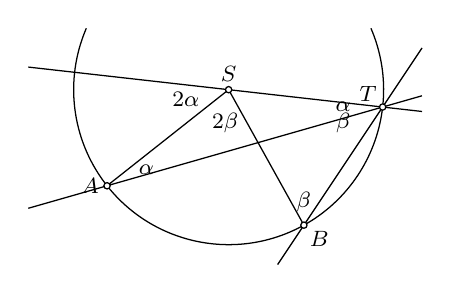
\begin{tikzpicture}
                    % \clip (0,0) rectangle (14.000000,10.000000);
                    {\footnotesize
                    
                    % Marking point T by circle
                    \draw [line width=0.016cm] (5.500000,3.000000) circle (0.040000);%
                    \draw (5.530000,2.970000) node [anchor=south east] { $T$ };%
                    
                    % Marking point A by circle
                    \draw [line width=0.016cm] (2.000000,2.000000) circle (0.040000);%
                    \draw (2.000000,2.000000) node [anchor=east] { $A$ };%
                    
                    % Marking point B by circle
                    \draw [line width=0.016cm] (4.500000,1.500000) circle (0.040000);%
                    \draw (4.470000,1.530000) node [anchor=north west] { $B$ };%
                    
                    % Drawing circle S A
                    \draw [line width=0.016cm] (2.025122,1.968874) -- (2.036326,1.955401) arc (220:297:1.968282 and 1.968282) -- (4.464838,1.480930);%
                    \draw [line width=0.016cm] (4.534767,1.519780) -- (4.557858,1.533441) arc (301:352:1.968282 and 1.968282) -- (5.495113,2.960299);%
                    \draw [line width=0.016cm] (5.504079,3.039791) -- (5.504910,3.049041) arc (355:360:1.968282 and 1.968282) --(5.512400,3.220588) arc (0:23:1.968282 and 1.968282) -- (5.351506,4.000000);%
                    \draw [line width=0.016cm] (1.736729,4.000000) -- (1.732304,3.989658) arc (157:217:1.968282 and 1.968282) -- (1.975515,2.031630);%
                    
                    % Drawing segment S B
                    \draw [line width=0.016cm] (3.563543,3.185622) -- (4.480574,1.534966);%
                    
                    % Drawing segment S A
                    \draw [line width=0.016cm] (3.512738,3.195783) -- (2.031380,2.024805);%
                    
                    % Drawing line T A
                    \draw [line width=0.016cm] (1.000000,1.714286) -- (1.961539,1.989011);%
                    \draw [line width=0.016cm] (2.038461,2.010989) -- (5.461539,2.989011);%
                    \draw [line width=0.016cm] (5.538461,3.010989) -- (6.000000,3.142857);%
                    
                    % Drawing line T B
                    \draw [line width=0.016cm] (4.166667,1.000000) -- (4.477812,1.466718);%
                    \draw [line width=0.016cm] (4.522188,1.533282) -- (5.477812,2.966718);%
                    \draw [line width=0.016cm] (5.522188,3.033282) -- (6.000000,3.750000);%
                    
                    % Drawing line T S
                    \draw [line width=0.016cm] (1.000000,3.507519) -- (3.504370,3.225071);%
                    \draw [line width=0.016cm] (3.583866,3.216105) -- (5.460252,3.004483);%
                    \draw [line width=0.016cm] (5.539748,2.995517) -- (6.000000,2.943609);%
                    
                    % Marking point S by circle
                    \draw [line width=0.016cm] (3.544118,3.220588) circle (0.040000);%
                    \draw (3.544118,3.220588) node [anchor=south] { $S$ };%
                    
                    % Marking point 2\alpha
                    \draw (3.000000,3.100000) node  { $2\alpha$ };%
                    
                    % Marking point \alpha
                    \draw (5.000000,3.000000) node  { $\alpha$ };%
                    
                    % Marking point \alpha
                    \draw (2.500000,2.200000) node  { $\alpha$ };%
                    
                    % Marking point 2\beta
                    \draw (3.500000,2.800000) node  { $2\beta$ };%
                    
                    % Marking point \beta
                    \draw (5.000000,2.800000) node  { $\beta$ };%
                    
                    % Marking point \beta
                    \draw (4.500000,1.800000) node  { $\beta$ };%
                    }
                    \end{tikzpicture}                    
                \\ $|\angle ATB|=\beta-\alpha$ in $|\angle ASB|=2\beta-2\alpha$
            \end{dokaz}

        \begin{posledica}[III.21]
            Vsi obodni koti nad izbranim lokom so skladni.
        \end{posledica}

        \begin{posledica}[III.22]
            Vsota mer nasprotnih kotov tetivnega štirikotnika je enaka $\pi$.
        \end{posledica}

            \begin{dokaz}
                \\ 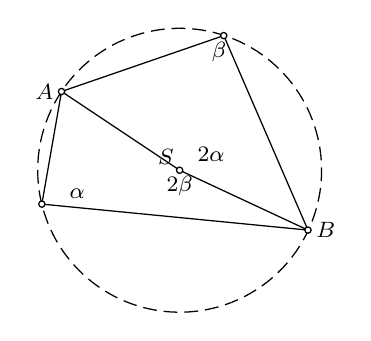
\begin{tikzpicture}
                    % \clip (0,0) rectangle (14.000000,10.000000);
                    {\footnotesize
                    
                    % Drawing segment A C
                    \draw [line width=0.016cm] (1.993111,3.960598) -- (1.756889,2.609402);%
                    
                    % Drawing segment A D
                    \draw [line width=0.016cm] (2.037817,4.013034) -- (4.022183,4.696966);%
                    
                    % Drawing segment D B
                    \draw [line width=0.016cm] (4.075900,4.673296) -- (5.114100,2.276704);%
                    
                    % Drawing segment C B
                    \draw [line width=0.016cm] (1.789811,2.566113) -- (5.090189,2.243887);%
                    
                    % Drawing segment A S
                    \draw [line width=0.016cm] (2.033282,3.977812) -- (3.466718,3.022188);%
                    
                    % Drawing segment S B
                    \draw [line width=0.016cm] (3.536253,2.983097) -- (5.093747,2.256903);%
                    
                    % Marking point C by circle
                    \draw [line width=0.016cm] (1.750000,2.570000) circle (0.040000);%
                    
                    % Marking point D by circle
                    \draw [line width=0.016cm] (4.060000,4.710000) circle (0.040000);%
                    
                    % Marking point A by circle
                    \draw [line width=0.016cm] (2.000000,4.000000) circle (0.040000);%
                    \draw (2.000000,4.000000) node [anchor=east] { $A$ };%
                    
                    % Marking point B by circle
                    \draw [line width=0.016cm] (5.130000,2.240000) circle (0.040000);%
                    \draw (5.130000,2.240000) node [anchor=west] { $B$ };%
                    
                    % Marking point S by circle
                    \draw [line width=0.016cm] (3.500000,3.000000) circle (0.040000);%
                    \draw (3.530000,2.970000) node [anchor=south east] { $S$ };%
                    
                    % Drawing circle S A
                    \draw [line width=0.016cm] (1.978183,3.966474) -- (1.971160,3.955326) arc (148:149:1.802776 and 1.802776) -- (1.953091,3.925783);%
                    \draw [line width=0.016cm] (1.953091,3.925783) -- (1.938751,3.901388) arc (150:151:1.802776 and 1.802776) -- (1.909852,3.849369);%
                    \draw [line width=0.016cm] (1.870384,3.770942) -- (1.866131,3.761886) arc (155:157:1.802776 and 1.802776) -- (1.834781,3.690685);%
                    \draw [line width=0.016cm] (1.834781,3.690685) -- (1.828496,3.675332) arc (158:160:1.802776 and 1.802776) -- (1.803128,3.608791);%
                    \draw [line width=0.016cm] (1.775500,3.525452) -- (1.767061,3.496913) arc (164:165:1.802776 and 1.802776) -- (1.751962,3.440867);%
                    \draw [line width=0.016cm] (1.751962,3.440867) -- (1.750775,3.436131) arc (166:168:1.802776 and 1.802776) -- (1.732570,3.355236);%
                    \draw [line width=0.016cm] (1.717371,3.268763) -- (1.714769,3.250898) arc (172:174:1.802776 and 1.802776) -- (1.706400,3.181653);%
                    \draw [line width=0.016cm] (1.706400,3.181653) -- (1.704084,3.157123) arc (175:177:1.802776 and 1.802776) -- (1.699682,3.094111);%
                    \draw [line width=0.016cm] (1.697236,3.006346) -- (1.697224,3.000000) arc (180:182:1.802776 and 1.802776) -- (1.699065,2.918566);%
                    \draw [line width=0.016cm] (1.699065,2.918567) -- (1.699695,2.905650) arc (183:185:1.802776 and 1.802776) -- (1.705165,2.830980);%
                    \draw [line width=0.016cm] (1.715523,2.743795) -- (1.719419,2.717984) arc (189:190:1.802776 and 1.802776) -- (1.730113,2.657217);%
                    \draw [line width=0.016cm] (1.730113,2.657217) -- (1.730346,2.656014) arc (191:192:1.802776 and 1.802776) -- (1.740186,2.608778);%
                    \draw [line width=0.016cm] (1.771843,2.486703) -- (1.775997,2.472920) arc (197:199:1.802776 and 1.802776) -- (1.798884,2.403172);%
                    \draw [line width=0.016cm] (1.798884,2.403172) -- (1.805945,2.383415) arc (200:202:1.802776 and 1.802776) -- (1.829959,2.321056);%
                    \draw [line width=0.016cm] (1.864996,2.240551) -- (1.866130,2.238114) arc (205:207:1.802776 and 1.802776) -- (1.903911,2.161848);%
                    \draw [line width=0.016cm] (1.903911,2.161848) -- (1.908243,2.153648) arc (208:210:1.802776 and 1.802776) -- (1.946611,2.085132);%
                    \draw [line width=0.016cm] (1.992996,2.010586) -- (2.005431,1.991901) arc (214:216:1.802776 and 1.802776) -- (2.042956,1.938387);%
                    \draw [line width=0.016cm] (2.042956,1.938387) -- (2.060239,1.915063) arc (217:218:1.802776 and 1.802776) -- (2.096371,1.868706);%
                    \draw [line width=0.016cm] (2.153116,1.801708) -- (2.160276,1.793708) arc (222:224:1.802776 and 1.802776) -- (2.213055,1.737553);%
                    \draw [line width=0.016cm] (2.213055,1.737553) -- (2.225245,1.725245) arc (225:227:1.802776 and 1.802776) -- (2.276047,1.676392);%
                    \draw [line width=0.016cm] (2.341942,1.618370) -- (2.365476,1.598980) arc (231:232:1.802776 and 1.802776) -- (2.410583,1.563626);%
                    \draw [line width=0.016cm] (2.410583,1.563626) -- (2.415062,1.560240) arc (233:235:1.802776 and 1.802776) -- (2.481809,1.512288);%
                    \draw [line width=0.016cm] (2.555450,1.464479) -- (2.571502,1.454720) arc (239:241:1.802776 and 1.802776) -- (2.631331,1.420312);%
                    \draw [line width=0.016cm] (2.631331,1.420312) -- (2.653648,1.408244) arc (242:243:1.802776 and 1.802776) -- (2.709272,1.379892);%
                    \draw [line width=0.016cm] (2.789089,1.343315) -- (2.795599,1.340536) arc (247:249:1.802776 and 1.802776) -- (2.870592,1.310667);%
                    \draw [line width=0.016cm] (2.870592,1.310667) -- (2.883414,1.305945) arc (250:252:1.802776 and 1.802776) -- (2.953588,1.282026);%
                    \draw [line width=0.016cm] (3.037880,1.257460) -- (3.063869,1.250775) arc (256:257:1.802776 and 1.802776) -- (3.123268,1.237027);%
                    \draw [line width=0.016cm] (3.123268,1.237027) -- (3.125181,1.236619) arc (258:260:1.802776 and 1.802776) -- (3.209550,1.220776);%
                    \draw [line width=0.016cm] (3.296521,1.208745) -- (3.311558,1.207100) arc (264:266:1.802776 and 1.802776) -- (3.383974,1.200962);%
                    \draw [line width=0.016cm] (3.383974,1.200962) -- (3.405650,1.199695) arc (267:269:1.802776 and 1.802776) -- (3.471702,1.197446);%
                    \draw [line width=0.016cm] (3.559498,1.198206) -- (3.562916,1.198323) arc (272:274:1.802776 and 1.802776) -- (3.647152,1.203240);%
                    \draw [line width=0.016cm] (3.647152,1.203240) -- (3.657122,1.204084) arc (275:277:1.802776 and 1.802776) -- (3.734458,1.212535);%
                    \draw [line width=0.016cm] (3.821207,1.226070) -- (3.843985,1.230346) arc (281:283:1.802776 and 1.802776) -- (3.907195,1.243813);%
                    \draw [line width=0.016cm] (3.907195,1.243813) -- (3.936130,1.250774) arc (284:285:1.802776 and 1.802776) -- (3.992216,1.265721);%
                    \draw [line width=0.016cm] (4.076070,1.291743) -- (4.086926,1.295442) arc (289:291:1.802776 and 1.802776) -- (4.158558,1.321816);%
                    \draw [line width=0.016cm] (4.158558,1.321816) -- (4.175331,1.328495) arc (292:294:1.802776 and 1.802776) -- (4.239484,1.355870);%
                    \draw [line width=0.016cm] (4.318656,1.393823) -- (4.346351,1.408243) arc (298:299:1.802776 and 1.802776) -- (4.395886,1.435587);%
                    \draw [line width=0.016cm] (4.395886,1.435587) -- (4.401387,1.438750) arc (300:302:1.802776 and 1.802776) -- (4.470991,1.481061);%
                    \draw [line width=0.016cm] (4.543793,1.530137) -- (4.559645,1.541524) arc (306:308:1.802776 and 1.802776) -- (4.614119,1.582700);%
                    \draw [line width=0.016cm] (4.614119,1.582700) -- (4.634523,1.598980) arc (309:310:1.802776 and 1.802776) -- (4.681803,1.638625);%
                    \draw [line width=0.016cm] (4.746683,1.697778) -- (4.752313,1.703191) arc (314:316:1.802776 and 1.802776) -- (4.808607,1.760021);%
                    \draw [line width=0.016cm] (4.808607,1.760021) -- (4.818466,1.770510) arc (317:319:1.802776 and 1.802776) -- (4.867426,1.825204);%
                    \draw [line width=0.016cm] (4.923003,1.893174) -- (4.939760,1.915062) arc (323:324:1.802776 and 1.802776) -- (4.975204,1.963769);%
                    \draw [line width=0.016cm] (4.975204,1.963769) -- (4.976747,1.965970) arc (325:327:1.802776 and 1.802776) -- (5.023906,2.036822);%
                    \draw [line width=0.016cm] (5.068993,2.112160) -- (5.076743,2.125997) arc (331:333:1.802776 and 1.802776) -- (5.110359,2.189603);%
                    \draw [line width=0.016cm] (5.110359,2.189603) arc (333:333:1.802776 and 1.802776) -- (5.116678,2.202283);%
                    \draw [line width=0.016cm] (5.181544,2.350069) -- (5.183036,2.353943) arc (339:341:1.802776 and 1.802776) -- (5.211193,2.432710);%
                    \draw [line width=0.016cm] (5.211193,2.432710) -- (5.214541,2.442911) arc (342:344:1.802776 and 1.802776) -- (5.236784,2.516696);%
                    \draw [line width=0.016cm] (5.258255,2.601829) -- (5.263381,2.625181) arc (348:350:1.802776 and 1.802776) -- (5.275556,2.687907);%
                    \draw [line width=0.016cm] (5.275556,2.687907) -- (5.280580,2.717983) arc (351:352:1.802776 and 1.802776) -- (5.288645,2.774724);%
                    \draw [line width=0.016cm] (5.297492,2.862076) -- (5.298384,2.874244) arc (356:358:1.802776 and 1.802776) -- (5.302075,2.949756);%
                    \draw [line width=0.016cm] (5.302075,2.949756) -- (5.302501,2.968537) arc (359:360:1.802776 and 1.802776) --(5.302776,3.000000) arc (0:1:1.802776 and 1.802776) -- (5.302384,3.037555);%
                    \draw [line width=0.016cm] (5.298418,3.125264) -- (5.298384,3.125755) arc (4:6:1.802776 and 1.802776) -- (5.290187,3.212676);%
                    \draw [line width=0.016cm] (5.290187,3.212676) -- (5.289338,3.219703) arc (7:9:1.802776 and 1.802776) -- (5.277709,3.299584);%
                    \draw [line width=0.016cm] (5.261015,3.385781) -- (5.256571,3.405536) arc (13:15:1.802776 and 1.802776) -- (5.240144,3.471063);%
                    \draw [line width=0.016cm] (5.240144,3.471063) -- (5.232939,3.496912) arc (16:17:1.802776 and 1.802776) -- (5.215145,3.555228);%
                    \draw [line width=0.016cm] (5.186078,3.638075) -- (5.183036,3.646057) arc (21:23:1.802776 and 1.802776) -- (5.153012,3.719410);%
                    \draw [line width=0.016cm] (5.153012,3.719410) -- (5.146918,3.733255) arc (24:26:1.802776 and 1.802776) -- (5.116026,3.799038);%
                    \draw [line width=0.016cm] (5.075206,3.876771) -- (5.061250,3.901388) arc (30:31:1.802776 and 1.802776) -- (5.030650,3.952424);%
                    \draw [line width=0.016cm] (5.030650,3.952424) -- (5.028840,3.955325) arc (32:34:1.802776 and 1.802776) -- (4.982463,4.025818);%
                    \draw [line width=0.016cm] (4.930761,4.096779) -- (4.920607,4.109899) arc (38:40:1.802776 and 1.802776) -- (4.875664,4.165139);%
                    \draw [line width=0.016cm] (4.875664,4.165139) -- (4.860572,4.182727) arc (41:43:1.802776 and 1.802776) -- (4.817305,4.230735);%
                    \draw [line width=0.016cm] (4.755821,4.293411) -- (4.752313,4.296808) arc (46:48:1.802776 and 1.802776) -- (4.691359,4.353020);%
                    \draw [line width=0.016cm] (4.691359,4.353020) -- (4.682727,4.360572) arc (49:51:1.802776 and 1.802776) -- (4.624071,4.409420);%
                    \draw [line width=0.016cm] (4.554116,4.462477) -- (4.534030,4.476747) arc (55:57:1.802776 and 1.802776) -- (4.481662,4.512065);%
                    \draw [line width=0.016cm] (4.481662,4.512065) -- (4.455326,4.528840) arc (58:59:1.802776 and 1.802776) -- (4.406879,4.558067);%
                    \draw [line width=0.016cm] (4.329945,4.600372) -- (4.318443,4.606285) arc (63:65:1.802776 and 1.802776) -- (4.251042,4.638883);%
                    \draw [line width=0.016cm] (4.251042,4.638883) -- (4.233255,4.646917) arc (66:68:1.802776 and 1.802776) -- (4.170358,4.673505);%
                    \draw [line width=0.016cm] (4.023017,4.725240) arc (73:73:1.802776 and 1.802776) -- (4.004415,4.730770);%
                    \draw [line width=0.016cm] (4.004415,4.730770) -- (3.996912,4.732939) arc (74:76:1.802776 and 1.802776) -- (3.919550,4.753276);%
                    \draw [line width=0.016cm] (3.833690,4.771624) -- (3.813049,4.775387) arc (80:82:1.802776 and 1.802776) -- (3.747038,4.785769);%
                    \draw [line width=0.016cm] (3.747038,4.785769) -- (3.719703,4.789338) arc (83:84:1.802776 and 1.802776) -- (3.659800,4.795679);%
                    \draw [line width=0.016cm] (3.572183,4.801330) -- (3.562916,4.801677) arc (88:90:1.802776 and 1.802776) -- (3.484395,4.802708);%
                    \draw [line width=0.016cm] (3.484395,4.802708) -- (3.468537,4.802501) arc (91:93:1.802776 and 1.802776) -- (3.396644,4.799810);%
                    \draw [line width=0.016cm] (3.309138,4.792644) -- (3.280297,4.789338) arc (97:98:1.802776 and 1.802776) -- (3.222085,4.781225);%
                    \draw [line width=0.016cm] (3.222085,4.781225) -- (3.217984,4.780581) arc (99:101:1.802776 and 1.802776) -- (3.135691,4.765582);%
                    \draw [line width=0.016cm] (3.050161,4.745751) -- (3.033407,4.741348) arc (105:107:1.802776 and 1.802776) -- (2.965698,4.721779);%
                    \draw [line width=0.016cm] (2.965698,4.721779) -- (2.942912,4.714542) arc (108:110:1.802776 and 1.802776) -- (2.882502,4.693723);%
                    \draw [line width=0.016cm] (2.800771,4.661650) -- (2.795600,4.659464) arc (113:115:1.802776 and 1.802776) -- (2.720699,4.625635);%
                    \draw [line width=0.016cm] (2.720699,4.625635) -- (2.709715,4.620324) arc (116:118:1.802776 and 1.802776) -- (2.642475,4.585765);%
                    \draw [line width=0.016cm] (2.566285,4.542134) -- (2.544675,4.528841) arc (122:123:1.802776 and 1.802776) -- (2.492309,4.494844);%
                    \draw [line width=0.016cm] (2.492309,4.494844) -- (2.491901,4.494569) arc (124:126:1.802776 and 1.802776) -- (2.420724,4.444009);%
                    \draw [line width=0.016cm] (2.351699,4.389750) -- (2.341198,4.381006) arc (130:132:1.802776 and 1.802776) -- (2.285397,4.332193);%
                    \draw [line width=0.016cm] (2.285397,4.332193) -- (2.270510,4.318467) arc (133:135:1.802776 and 1.802776) -- (2.221976,4.271477);%
                    \draw [line width=0.016cm] (2.161586,4.207746) -- (2.160277,4.206293) arc (138:140:1.802776 and 1.802776) -- (2.104372,4.141149);%
                    \draw [line width=0.016cm] (2.104372,4.141149) -- (2.098980,4.134524) arc (141:143:1.802776 and 1.802776) -- (2.050467,4.071846);%
                    
                    % Marking point \alpha
                    \draw (2.200000,2.700000) node  { $\alpha$ };%
                    
                    % Marking point \beta
                    \draw (4.000000,4.500000) node  { $\beta$ };%
                    
                    % Marking point 2\alpha
                    \draw (3.900000,3.200000) node  { $2\alpha$ };%
                    
                    % Marking point 2\beta
                    \draw (3.500000,2.800000) node  { $2\beta$ };%
                    }
                    \end{tikzpicture}                    
                \\ $2\alpha+2\beta=2\pi \Rightarrow \alpha+\beta=\pi$
            \end{dokaz}

        \begin{trditev}[III.31 -- Talesov izrek]
            Kot, včrtav v polkrog, je pravi kot.
        \end{trditev}

            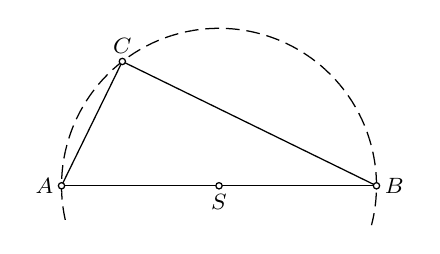
\begin{tikzpicture}
                % \clip (0,0) rectangle (14.000000,10.000000);
                {\footnotesize
                
                % Drawing segment A C
                \draw [line width=0.016cm] (1.517576,2.535932) -- (2.254728,4.042917);%
                
                % Drawing segment A B
                \draw [line width=0.016cm] (1.540000,2.500000) -- (3.460000,2.500000);%
                \draw [line width=0.016cm] (3.540000,2.500000) -- (5.460000,2.500000);%
                
                % Drawing segment C B
                \draw [line width=0.016cm] (2.308235,4.061272) -- (5.464068,2.517576);%
                
                % Marking point C by circle
                \draw [line width=0.016cm] (2.272304,4.078848) circle (0.040000);%
                \draw (2.272304,4.078848) node [anchor=south] { $C$ };%
                
                % Marking point A by circle
                \draw [line width=0.016cm] (1.500000,2.500000) circle (0.040000);%
                \draw (1.500000,2.500000) node [anchor=east] { $A$ };%
                
                % Marking point B by circle
                \draw [line width=0.016cm] (5.500000,2.500000) circle (0.040000);%
                \draw (5.500000,2.500000) node [anchor=west] { $B$ };%
                
                % Marking point S by circle
                \draw [line width=0.016cm] (3.500000,2.500000) circle (0.040000);%
                \draw (3.500000,2.500000) node [anchor=north] { $S$ };%
                
                % Drawing circle S A
                \draw [line width=0.016cm] (1.500400,2.460003) -- (1.501218,2.430201) arc (182:182:2.000000 and 2.000000) -- (1.501904,2.412762);%
                \draw [line width=0.016cm] (1.501904,2.412762) -- (1.502741,2.395328) arc (183:184:2.000000 and 2.000000) -- (1.507611,2.325689);%
                \draw [line width=0.016cm] (1.517110,2.238948) -- (1.519464,2.221654) arc (188:189:2.000000 and 2.000000) -- (1.530384,2.152704);%
                \draw [line width=0.016cm] (1.530384,2.152704) -- (1.530384,2.152704) arc (190:192:2.000000 and 2.000000) -- (1.547408,2.067121);%
                \draw [line width=0.016cm] (5.436492,1.999999) -- (5.440591,2.016156) arc (346:347:2.000000 and 2.000000) -- (5.452592,2.067120);%
                \draw [line width=0.016cm] (5.452592,2.067120) -- (5.456295,2.084176) arc (348:349:2.000000 and 2.000000) -- (5.469615,2.152703);%
                \draw [line width=0.016cm] (5.482890,2.238947) -- (5.485092,2.256261) arc (353:354:2.000000 and 2.000000) -- (5.492389,2.325688);%
                \draw [line width=0.016cm] (5.492389,2.325688) -- (5.492389,2.325688) arc (355:357:2.000000 and 2.000000) -- (5.498096,2.412760);%
                \draw [line width=0.016cm] (5.499600,2.539998) -- (5.498782,2.569799) arc (2:2:2.000000 and 2.000000) -- (5.498096,2.587238);%
                \draw [line width=0.016cm] (5.498096,2.587238) -- (5.497259,2.604672) arc (3:4:2.000000 and 2.000000) -- (5.492389,2.674311);%
                \draw [line width=0.016cm] (5.482890,2.761052) -- (5.480536,2.778346) arc (8:9:2.000000 and 2.000000) -- (5.469616,2.847296);%
                \draw [line width=0.016cm] (5.469616,2.847296) -- (5.469616,2.847296) arc (10:12:2.000000 and 2.000000) -- (5.452592,2.932879);%
                \draw [line width=0.016cm] (5.431852,3.017638) -- (5.431852,3.017638) arc (15:17:2.000000 and 2.000000) -- (5.407434,3.101411);%
                \draw [line width=0.016cm] (5.407434,3.101411) -- (5.402113,3.118034) arc (18:19:2.000000 and 2.000000) -- (5.379385,3.184040);%
                \draw [line width=0.016cm] (5.347759,3.265367) -- (5.341010,3.281462) arc (23:24:2.000000 and 2.000000) -- (5.312616,3.345236);%
                \draw [line width=0.016cm] (5.312616,3.345236) -- (5.312616,3.345236) arc (25:27:2.000000 and 2.000000) -- (5.274022,3.423497);%
                \draw [line width=0.016cm] (5.232051,3.500000) -- (5.232051,3.500000) arc (30:32:2.000000 and 2.000000) -- (5.186783,3.574599);%
                \draw [line width=0.016cm] (5.186783,3.574599) -- (5.177341,3.589278) arc (33:34:2.000000 and 2.000000) -- (5.138304,3.647153);%
                \draw [line width=0.016cm] (5.086707,3.717523) -- (5.076022,3.731323) arc (38:39:2.000000 and 2.000000) -- (5.032089,3.785575);%
                \draw [line width=0.016cm] (5.032089,3.785575) -- (5.032089,3.785575) arc (40:42:2.000000 and 2.000000) -- (4.974555,3.851180);%
                \draw [line width=0.016cm] (4.914214,3.914213) -- (4.914214,3.914214) arc (45:47:2.000000 and 2.000000) -- (4.851181,3.974554);%
                \draw [line width=0.016cm] (4.851181,3.974554) -- (4.838261,3.986290) arc (48:49:2.000000 and 2.000000) -- (4.785576,4.032089);%
                \draw [line width=0.016cm] (4.717523,4.086706) -- (4.703630,4.097271) arc (53:54:2.000000 and 2.000000) -- (4.647153,4.138304);%
                \draw [line width=0.016cm] (4.647153,4.138304) -- (4.647153,4.138304) arc (55:57:2.000000 and 2.000000) -- (4.574600,4.186783);%
                \draw [line width=0.016cm] (4.500000,4.232051) -- (4.500000,4.232051) arc (60:62:2.000000 and 2.000000) -- (4.423498,4.274021);%
                \draw [line width=0.016cm] (4.423498,4.274021) -- (4.407981,4.282013) arc (63:64:2.000000 and 2.000000) -- (4.345237,4.312615);%
                \draw [line width=0.016cm] (4.265367,4.347759) -- (4.249213,4.354368) arc (68:69:2.000000 and 2.000000) -- (4.184041,4.379385);%
                \draw [line width=0.016cm] (4.184041,4.379385) -- (4.184040,4.379385) arc (70:72:2.000000 and 2.000000) -- (4.101412,4.407434);%
                \draw [line width=0.016cm] (4.017639,4.431852) -- (4.017638,4.431852) arc (75:77:2.000000 and 2.000000) -- (3.932880,4.452592);%
                \draw [line width=0.016cm] (3.932880,4.452592) -- (3.915824,4.456295) arc (78:79:2.000000 and 2.000000) -- (3.847297,4.469615);%
                \draw [line width=0.016cm] (3.761053,4.482890) -- (3.743739,4.485092) arc (83:84:2.000000 and 2.000000) -- (3.674312,4.492389);%
                \draw [line width=0.016cm] (3.674312,4.492389) -- (3.674312,4.492389) arc (85:87:2.000000 and 2.000000) -- (3.587239,4.498096);%
                \draw [line width=0.016cm] (3.500000,4.500000) -- (3.500000,4.500000) arc (90:92:2.000000 and 2.000000) -- (3.412762,4.498096);%
                \draw [line width=0.016cm] (3.412762,4.498096) -- (3.395328,4.497259) arc (93:94:2.000000 and 2.000000) -- (3.325689,4.492389);%
                \draw [line width=0.016cm] (3.238948,4.482890) -- (3.221654,4.480536) arc (98:99:2.000000 and 2.000000) -- (3.152704,4.469616);%
                \draw [line width=0.016cm] (3.152704,4.469616) -- (3.152704,4.469616) arc (100:102:2.000000 and 2.000000) -- (3.067121,4.452592);%
                \draw [line width=0.016cm] (2.982362,4.431852) -- (2.982362,4.431852) arc (105:107:2.000000 and 2.000000) -- (2.898589,4.407434);%
                \draw [line width=0.016cm] (2.898589,4.407434) -- (2.881966,4.402113) arc (108:109:2.000000 and 2.000000) -- (2.815960,4.379385);%
                \draw [line width=0.016cm] (2.734634,4.347759) -- (2.718538,4.341010) arc (113:114:2.000000 and 2.000000) -- (2.654764,4.312616);%
                \draw [line width=0.016cm] (2.654764,4.312616) -- (2.654764,4.312616) arc (115:117:2.000000 and 2.000000) -- (2.576503,4.274022);%
                \draw [line width=0.016cm] (2.500000,4.232051) -- (2.500000,4.232051) arc (120:122:2.000000 and 2.000000) -- (2.425401,4.186783);%
                \draw [line width=0.016cm] (2.425401,4.186783) -- (2.410722,4.177341) arc (123:124:2.000000 and 2.000000) -- (2.352848,4.138304);%
                \draw [line width=0.016cm] (2.240974,4.053980) arc (129:129:2.000000 and 2.000000) -- (2.214425,4.032089);%
                \draw [line width=0.016cm] (2.214425,4.032089) -- (2.214425,4.032089) arc (130:132:2.000000 and 2.000000) -- (2.148820,3.974555);%
                \draw [line width=0.016cm] (2.085787,3.914214) -- (2.085787,3.914214) arc (135:137:2.000000 and 2.000000) -- (2.025446,3.851181);%
                \draw [line width=0.016cm] (2.025446,3.851181) -- (2.013711,3.838261) arc (138:139:2.000000 and 2.000000) -- (1.967911,3.785576);%
                \draw [line width=0.016cm] (1.913294,3.717523) -- (1.902729,3.703630) arc (143:144:2.000000 and 2.000000) -- (1.861696,3.647153);%
                \draw [line width=0.016cm] (1.861696,3.647153) -- (1.861696,3.647153) arc (145:147:2.000000 and 2.000000) -- (1.813217,3.574600);%
                \draw [line width=0.016cm] (1.767949,3.500000) -- (1.767949,3.500000) arc (150:152:2.000000 and 2.000000) -- (1.725979,3.423498);%
                \draw [line width=0.016cm] (1.725979,3.423498) -- (1.717987,3.407981) arc (153:154:2.000000 and 2.000000) -- (1.687385,3.345237);%
                \draw [line width=0.016cm] (1.652241,3.265367) -- (1.645632,3.249213) arc (158:159:2.000000 and 2.000000) -- (1.620615,3.184041);%
                \draw [line width=0.016cm] (1.620615,3.184041) -- (1.620615,3.184041) arc (160:162:2.000000 and 2.000000) -- (1.592566,3.101412);%
                \draw [line width=0.016cm] (1.568148,3.017639) -- (1.568148,3.017638) arc (165:167:2.000000 and 2.000000) -- (1.547408,2.932880);%
                \draw [line width=0.016cm] (1.547408,2.932880) -- (1.543705,2.915824) arc (168:169:2.000000 and 2.000000) -- (1.530385,2.847297);%
                \draw [line width=0.016cm] (1.517110,2.761053) -- (1.514908,2.743739) arc (173:174:2.000000 and 2.000000) -- (1.507611,2.674312);%
                \draw [line width=0.016cm] (1.507611,2.674312) -- (1.507611,2.674312) arc (175:177:2.000000 and 2.000000) -- (1.501904,2.587239);%
                }
            \end{tikzpicture}

        \begin{trditev}[III.35, III.36 -- potenca točke na krožnico]
            Naj bo dana kožnica $K$ in točka $A\notin K$.
            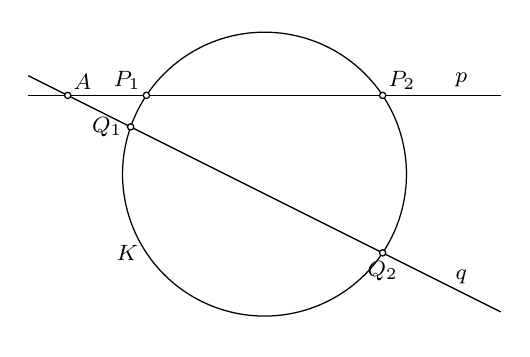
\begin{tikzpicture}
                % \clip (0,0) rectangle (14.000000,10.000000);
                {\footnotesize
                
                % Marking point p
                \draw (6.500000,4.000000) node [anchor=south] { $p$ };%
                
                % Marking point q
                \draw (6.500000,1.500000) node [anchor=south] { $q$ };%
                
                % Marking point A by circle
                \draw [line width=0.016cm] (1.500000,4.000000) circle (0.040000);%
                \draw (1.470000,3.970000) node [anchor=south west] { $A$ };%
                
                % Marking point P_1 by circle
                \draw [line width=0.016cm] (2.500000,4.000000) circle (0.040000);%
                \draw (2.530000,3.970000) node [anchor=south east] { $P_1$ };%
                
                % Marking point P_2 by circle
                \draw [line width=0.016cm] (5.500000,4.000000) circle (0.040000);%
                \draw (5.470000,3.970000) node [anchor=south west] { $P_2$ };%
                
                % Marking point Q_1 by circle
                \draw [line width=0.016cm] (2.300000,3.600000) circle (0.040000);%
                \draw (2.300000,3.600000) node [anchor=east] { $Q_1$ };%
                
                % Marking point Q_2 by circle
                \draw [line width=0.016cm] (5.500000,2.000000) circle (0.040000);%
                \draw (5.500000,2.000000) node [anchor=north] { $Q_2$ };%
                
                % Marking point K
                \draw (2.500000,2.000000) node [anchor=east] { $K$ };%
                
                % Drawing line P
                \draw [line width=0.016cm] (1.000000,4.000000) -- (1.460000,4.000000);%
                \draw [line width=0.016cm] (1.540000,4.000000) -- (2.460000,4.000000);%
                \draw [line width=0.016cm] (2.540000,4.000000) -- (5.460000,4.000000);%
                \draw [line width=0.016cm] (5.540000,4.000000) -- (7.000000,4.000000);%
                
                % Drawing line Q
                \draw [line width=0.016cm] (1.000000,4.250000) -- (1.464223,4.017889);%
                \draw [line width=0.016cm] (1.535777,3.982111) -- (2.264223,3.617889);%
                \draw [line width=0.016cm] (2.335777,3.582111) -- (5.464223,2.017889);%
                \draw [line width=0.016cm] (5.535777,1.982111) -- (7.000000,1.250000);%
                
                % Drawing circle k
                \draw [line width=0.016cm] (5.802776,3.000000) arc (0:32:1.802776 and 1.802776) -- (5.521817,3.966474);%
                \draw [line width=0.016cm] (5.477444,4.033034) -- (5.476747,4.034030) arc (35:145:1.802776 and 1.802776) -- (2.522556,4.033034);%
                \draw [line width=0.016cm] (2.478183,3.966474) -- (2.471160,3.955326) arc (148:159:1.802776 and 1.802776) -- (2.313730,3.637570);%
                \draw [line width=0.016cm] (2.287106,3.562135) -- (2.285459,3.557089) arc (162:325:1.802776 and 1.802776) -- (5.477444,1.966966);%
                \draw [line width=0.016cm] (5.521817,2.033526) -- (5.528840,2.044674) arc (328:359:1.802776 and 1.802776) -- (5.802776,2.999999);%
                }
            \end{tikzpicture}                
            \begin{enumerate}
                \item Če premici $p$ in $q$ skozi $A$ sekata krožnico $K$ v točkah $P_1, P_2$ oziroma $Q_1, Q_2$, potem je: $|AP_1|\cdot|AP_2|=|AQ_1|\cdot|AQ_2|$.
                \item Če točka $A$ leži izven krožnice $K$, potem je premica $p$ skozi $A$ tangenta na krožnico $K$ v točki $T$ natanko takrat, ko je: $|AT|^2=potenca~A~na~K$.
            \end{enumerate}
        \end{trditev}
        
            \begin{dokaz}
                    \\ (1)
                    \\ $\circ $ \uline{$A$ leži izven $K$:} 
                    \\ 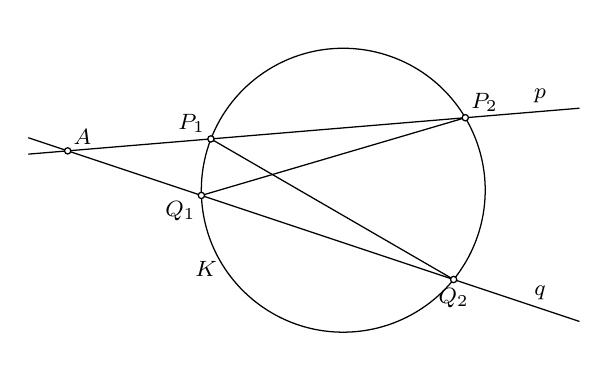
\begin{tikzpicture}
                        % \clip (0,0) rectangle (14.000000,10.000000);
                        {\footnotesize
                        
                        % Marking point p
                        \draw (7.500000,4.000000) node [anchor=south] { $p$ };%
                        
                        % Marking point q
                        \draw (7.500000,1.500000) node [anchor=south] { $q$ };%
                        
                        % Marking point A by circle
                        \draw [line width=0.016cm] (1.500000,3.500000) circle (0.040000);%
                        \draw (1.470000,3.470000) node [anchor=south west] { $A$ };%
                        
                        % Marking point P_1 by circle
                        \draw [line width=0.016cm] (3.319099,3.651592) circle (0.040000);%
                        \draw (3.349099,3.621592) node [anchor=south east] { $P_1$ };%
                        
                        % Marking point P_2 by circle
                        \draw [line width=0.016cm] (6.549867,3.920822) circle (0.040000);%
                        \draw (6.519867,3.890822) node [anchor=south west] { $P_2$ };%
                        
                        % Marking point Q_1 by circle
                        \draw [line width=0.016cm] (3.198438,2.933854) circle (0.040000);%
                        \draw (3.228438,2.963854) node [anchor=north east] { $Q_1$ };%
                        
                        % Marking point Q_2 by circle
                        \draw [line width=0.016cm] (6.401562,1.866146) circle (0.040000);%
                        \draw (6.401562,1.866146) node [anchor=north] { $Q_2$ };%
                        
                        % Marking point K
                        \draw (3.500000,2.000000) node [anchor=east] { $K$ };%
                        
                        % Drawing line P
                        \draw [line width=0.016cm] (1.000000,3.458333) -- (1.460138,3.496678);%
                        \draw [line width=0.016cm] (1.539862,3.503322) -- (3.279237,3.648270);%
                        \draw [line width=0.016cm] (3.358961,3.654913) -- (6.510005,3.917500);%
                        \draw [line width=0.016cm] (6.589728,3.924144) -- (8.000000,4.041667);%
                        
                        % Drawing line Q
                        \draw [line width=0.016cm] (1.000000,3.666667) -- (1.462053,3.512649);%
                        \draw [line width=0.016cm] (1.537947,3.487351) -- (3.160491,2.946503);%
                        \draw [line width=0.016cm] (3.236386,2.921205) -- (6.363614,1.878795);%
                        \draw [line width=0.016cm] (6.439509,1.853497) -- (8.000000,1.333333);%
                        
                        % Drawing circle k
                        \draw [line width=0.016cm] (6.802776,3.000000) arc (0:29:1.802776 and 1.802776) -- (6.569915,3.886209);%
                        \draw [line width=0.016cm] (6.529055,3.954982) -- (6.528840,3.955325) arc (32:157:1.802776 and 1.802776) -- (3.333969,3.688725);%
                        \draw [line width=0.016cm] (3.305056,3.614138) -- (3.295442,3.586927) arc (161:180:1.802776 and 1.802776) -- (3.197414,2.973841);%
                        \draw [line width=0.016cm] (3.200349,2.893900) -- (3.201616,2.874245) arc (184:319:1.802776 and 1.802776) -- (6.376060,1.835329);%
                        \draw [line width=0.016cm] (6.426373,1.897521) -- (6.439760,1.915062) arc (323:359:1.802776 and 1.802776) -- (6.802776,2.999999);%
                        
                        % Drawing segment Q_1 P_2
                        \draw [line width=0.016cm] (3.236809,2.945154) -- (6.511496,3.909522);%
                        
                        % Drawing segment P_1 Q_2
                        \draw [line width=0.016cm] (3.353712,3.631543) -- (6.366949,1.886195);%
                        }
                        \end{tikzpicture}                        
                    \\ Velja: $\angle P_2\cong \angle Q_2$, saj sta oba kota obodna nad istim lokom ($\arc{P_1Q_1}$). Potem velja podobnost: $\triangle AP_2Q_1 \sim \triangle AQ_2P_1$ po KKK, saj imata dva skladna kota (zato je tudi tretji kot skladen). To pomeni, da so razmerja istoležnih stranic enaka: $\frac{|AP_2|}{|AQ_2|}=\frac{|AQ_1|}{|AP_1|} \rightarrow |AP_1|\cdot|AP_2|=|AQ_1|\cdot|AQ_2|$
                    \\ $\circ \circ $ \uline{$A$ leži znotraj $K$:}  
                    \\ 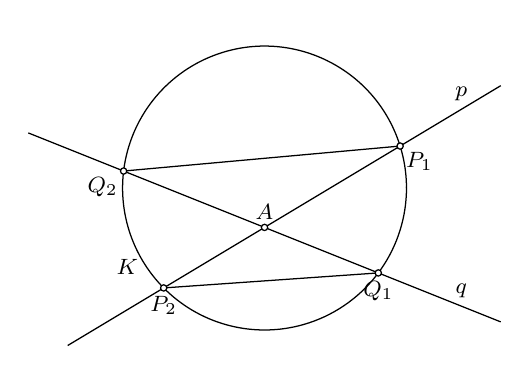
\begin{tikzpicture}
                        % \clip (0,0) rectangle (14.000000,10.000000);
                        {\footnotesize
                        
                        % Marking point p
                        \draw (7.500000,4.000000) node [anchor=south] { $p$ };%
                        
                        % Marking point q
                        \draw (7.500000,1.500000) node [anchor=south] { $q$ };%
                        
                        % Marking point A by circle
                        \draw [line width=0.016cm] (5.000000,2.500000) circle (0.040000);%
                        \draw (5.000000,2.500000) node [anchor=south] { $A$ };%
                        
                        % Marking point P_1 by circle
                        \draw [line width=0.016cm] (6.722101,3.533261) circle (0.040000);%
                        \draw (6.692101,3.563261) node [anchor=north west] { $P_1$ };%
                        
                        % Marking point P_2 by circle
                        \draw [line width=0.016cm] (3.719075,1.731445) circle (0.040000);%
                        \draw (3.719075,1.731445) node [anchor=north] { $P_2$ };%
                        
                        % Marking point Q_1 by circle
                        \draw [line width=0.016cm] (6.444971,1.922012) circle (0.040000);%
                        \draw (6.444971,1.922012) node [anchor=north] { $Q_1$ };%
                        
                        % Marking point Q_2 by circle
                        \draw [line width=0.016cm] (3.210201,3.215919) circle (0.040000);%
                        \draw (3.240201,3.245919) node [anchor=north east] { $Q_2$ };%
                        
                        % Marking point K
                        \draw (3.500000,2.000000) node [anchor=east] { $K$ };%
                        
                        % Drawing line P
                        \draw [line width=0.016cm] (2.500000,1.000000) -- (3.684775,1.710865);%
                        \draw [line width=0.016cm] (3.753375,1.752025) -- (4.965700,2.479420);%
                        \draw [line width=0.016cm] (5.034300,2.520580) -- (6.687802,3.512681);%
                        \draw [line width=0.016cm] (6.756401,3.553841) -- (8.000000,4.300000);%
                        
                        % Drawing line Q
                        \draw [line width=0.016cm] (2.000000,3.700000) -- (3.173062,3.230775);%
                        \draw [line width=0.016cm] (3.247341,3.201064) -- (4.962861,2.514856);%
                        \draw [line width=0.016cm] (5.037139,2.485144) -- (6.407832,1.936867);%
                        \draw [line width=0.016cm] (6.482110,1.907156) -- (8.000000,1.300000);%
                        
                        % Drawing circle k
                        \draw [line width=0.016cm] (6.802776,3.000000) arc (0:15:1.802776 and 1.802776) -- (6.733509,3.494922);%
                        \draw [line width=0.016cm] (6.709846,3.571337) -- (6.704558,3.586926) arc (19:171:1.802776 and 1.802776) -- (3.215433,3.255576);%
                        \draw [line width=0.016cm] (3.205852,3.176157) -- (3.204084,3.157123) arc (175:223:1.802776 and 1.802776) -- (3.691245,1.760177);%
                        \draw [line width=0.016cm] (3.747535,1.703338) -- (3.747687,1.703192) arc (226:322:1.802776 and 1.802776) -- (6.420698,1.890217);%
                        \draw [line width=0.016cm] (6.468532,1.954336) -- (6.476747,1.965970) arc (325:360:1.802776 and 1.802776) --(6.802776,3.000000) arc (0:0:1.802776 and 1.802776);%
                        
                        % Drawing segment Q_1 P_2
                        \draw [line width=0.016cm] (6.405068,1.919222) -- (3.758978,1.734235);%
                        
                        % Drawing segment P_1 Q_2
                        \draw [line width=0.016cm] (6.682264,3.529661) -- (3.250039,3.219519);%
                        }
                        \end{tikzpicture}
                    \\ Velja $\triangle AP_1Q_2 \sim \triangle AQ_1P_2$. Iz tega sledi: $\frac{|AP_2|}{|AQ_2|}=\frac{|AQ_1|}{|AP_1|} \rightarrow |AP_1|\cdot|AP_2|=|AQ_1|\cdot|AQ_2|$.
                    \\ (2)
                    \\ ($\Rightarrow$): 
                    \\ 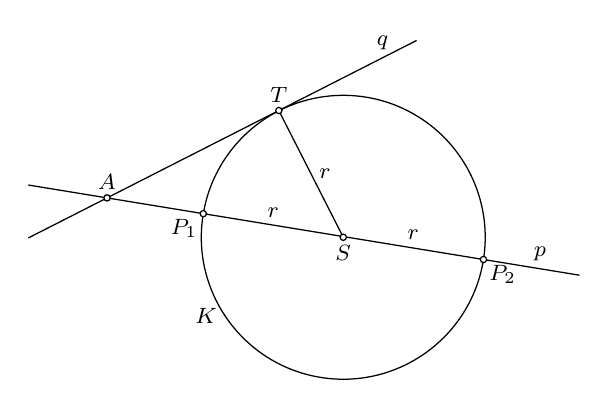
\begin{tikzpicture}
                        % \clip (0,0) rectangle (14.000000,10.000000);
                        {\footnotesize
                        
                        % Marking point p
                        \draw (7.500000,2.600000) node [anchor=south] { $p$ };%
                        
                        % Marking point q
                        \draw (5.500000,5.280000) node [anchor=south] { $q$ };%
                        
                        % Marking point A by circle
                        \draw [line width=0.016cm] (2.000000,3.500000) circle (0.040000);%
                        \draw (2.000000,3.500000) node [anchor=south] { $A$ };%
                        
                        % Marking point P_1 by circle
                        \draw [line width=0.016cm] (3.222357,3.299978) circle (0.040000);%
                        \draw (3.252357,3.329978) node [anchor=north east] { $P_1$ };%
                        
                        % Marking point P_2 by circle
                        \draw [line width=0.016cm] (6.780540,2.717730) circle (0.040000);%
                        \draw (6.750540,2.747730) node [anchor=north west] { $P_2$ };%
                        
                        % Marking point K
                        \draw (3.500000,2.000000) node [anchor=east] { $K$ };%
                        
                        % Drawing line P
                        \draw [line width=0.016cm] (1.000000,3.663636) -- (1.960525,3.506460);%
                        \draw [line width=0.016cm] (2.039475,3.493540) -- (3.182882,3.306437);%
                        \draw [line width=0.016cm] (3.261832,3.293518) -- (4.962980,3.015149);%
                        \draw [line width=0.016cm] (5.039918,3.002559) -- (6.741065,2.724189);%
                        \draw [line width=0.016cm] (6.820015,2.711270) -- (8.000000,2.518182);%
                        
                        % Drawing line Q
                        \draw [line width=0.016cm] (5.932584,5.500000) -- (4.217138,4.627573);%
                        \draw [line width=0.016cm] (4.145830,4.591308) -- (2.035654,3.518133);%
                        \draw [line width=0.016cm] (1.964346,3.481867) -- (1.000000,2.991429);%
                        
                        % Drawing circle k
                        \draw [line width=0.016cm] (6.802776,3.000000) arc (0:115:1.802776 and 1.802776) -- (4.218508,4.624583);%
                        \draw [line width=0.016cm] (4.147441,4.588440) -- (4.125997,4.576743) arc (119:169:1.802776 and 1.802776) -- (3.229450,3.339344);%
                        \draw [line width=0.016cm] (3.216139,3.260464) -- (3.214769,3.250898) arc (172:349:1.802776 and 1.802776) -- (6.773839,2.678295);%
                        \draw [line width=0.016cm] (6.786365,2.757303) -- (6.789338,2.780296) arc (353:360:1.802776 and 1.802776) --(6.802776,3.000000) arc (0:0:1.802776 and 1.802776);%
                        
                        % Marking point T by circle
                        \draw [line width=0.016cm] (4.181484,4.609441) circle (0.040000);%
                        \draw (4.181484,4.609441) node [anchor=south] { $T$ };%
                        
                        % Marking point S by circle
                        \draw [line width=0.016cm] (5.000000,3.000000) circle (0.040000);%
                        \draw (5.000000,3.000000) node [anchor=north] { $S$ };%
                        
                        % Drawing segment T S
                        \draw [line width=0.016cm] (4.199617,4.573787) -- (4.981867,3.035654);%
                        
                        % Marking point r
                        \draw (4.111179,3.149989) node [anchor=south] { $r$ };%
                        
                        % Marking point r
                        \draw (5.890270,2.858865) node [anchor=south] { $r$ };%
                        
                        % Marking point r
                        \draw (4.590742,3.804720) node [anchor=west] { $r$ };%
                        }
                        \end{tikzpicture}                        
                    \\ Naj bo $S$ središče krožnice $K$, $\overleftrightarrow{AS}$ naj seka $K$ v točkah $P_1, P_2$ in velja $|AP_1|\cdot|AP_2|=potenca~A~na~K$. Ker je polmer pravokoten na tangento, je trikotnik $\triangle AST$ pravokoten. Potem velja: $|AS|^2=|AT|^2+r^2 \rightarrow |AT|^2=|AS|^2-r^2=(|AS|-r)(|AS|+r)=|AP_1|\cdot |AP_2|=potenca$.
                    \\ ($\Leftarrow$): 
                    \\ 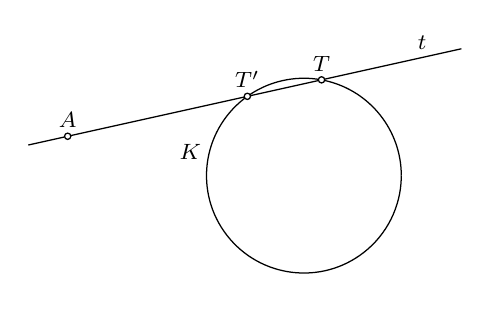
\begin{tikzpicture}
                        % \clip (0,0) rectangle (14.000000,10.000000);
                        {\footnotesize
                        
                        % Marking point t
                        \draw (6.500000,5.000000) node [anchor=south] { $t$ };%
                        
                        % Marking point A by circle
                        \draw [line width=0.016cm] (2.000000,4.000000) circle (0.040000);%
                        \draw (2.000000,4.000000) node [anchor=south] { $A$ };%
                        
                        % Marking point T' by circle
                        \draw [line width=0.016cm] (4.281794,4.507065) circle (0.040000);%
                        \draw (4.281794,4.507065) node [anchor=south] { $T'$ };%
                        
                        % Marking point T by circle
                        \draw [line width=0.016cm] (5.224088,4.716464) circle (0.040000);%
                        \draw (5.224088,4.716464) node [anchor=south] { $T$ };%
                        
                        % Marking point K
                        \draw (3.800000,3.800000) node [anchor=east] { $K$ };%
                        
                        % Drawing line P
                        \draw [line width=0.016cm] (1.500000,3.888889) -- (1.960953,3.991323);%
                        \draw [line width=0.016cm] (2.039047,4.008677) -- (4.242747,4.498388);%
                        \draw [line width=0.016cm] (4.320842,4.515743) -- (5.185040,4.707787);%
                        \draw [line width=0.016cm] (5.263135,4.725141) -- (7.000000,5.111111);%
                        
                        % Drawing circle k
                        \draw [line width=0.016cm] (6.236932,3.500000) arc (0:77:1.236932 and 1.236932) -- (5.263304,4.708582);%
                        \draw [line width=0.016cm] (5.184638,4.723074) -- (5.172148,4.724894) arc (82:123:1.236932 and 1.236932) -- (4.314732,4.529761);%
                        \draw [line width=0.016cm] (4.249608,4.483317) -- (4.238469,4.474716) arc (128:359:1.236932 and 1.236932) -- (6.236932,3.500000);%
                        }
                        \end{tikzpicture}                        
                    \\ Če je $|AT|^2=potenca~A~na~K$, dokazujemo, da je $t$ tangenta na $K$. Če to ne velja, potem $t$ seka $K$ še v točki $T'$, torej je: $|AT|\cdot|AT'|=potenca=|AT|^2$. Iz tega sledi: $|AT|=|AT'|\Rightarrow T=T'$, kar pa je protislovje.
                \end{dokaz}

        \begin{definicija}
            Če je točka $A$ izven krožnice $K$, to vrednost imenujemo \textbf{potenca točke} $A$ na krožnico $K$. Če je $A$ znotraj krožnice $K$, potem nasprotno vrednost tega produkta imenujemo potenca točke $A$ na krožnico $K$.
        \end{definicija}


\section{Geometrija inverzij}

    \begin{definicija}
        Naj bo dana krožnica $K$ s središčem $S$ in polmerom $r$.
        Za poljubno točko $A\neq S$ je njen \textbf{inverz} v $K$ enak točki $A'\in \overrightarrow{SA}$, za katero velja $|SA|\cdot|SA'|=r^2$. 
        Pripadajočo preslikavo ravnine brez točke $S$ imenujemo \textbf{inverzija}.
    \end{definicija}

        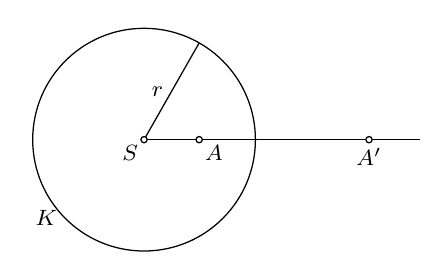
\begin{tikzpicture}
            % \clip (0,0) rectangle (14.000000,10.000000);
            {\footnotesize
            
            % Drawing circle k
            \draw [line width=0.016cm] (2.500000,2.500000) circle (1.414214);%
            
            % Drawing segment S U
            \draw [line width=0.016cm] (2.540000,2.500000) -- (3.160000,2.500000);%
            \draw [line width=0.016cm] (3.240000,2.500000) -- (5.317143,2.500000);%
            \draw [line width=0.016cm] (5.397143,2.500000) -- (6.000000,2.500000);%
            
            % Drawing segment S B
            \draw [line width=0.016cm] (2.519799,2.534756) -- (3.200000,3.728821);%
            
            % Marking point S by circle
            \draw [line width=0.016cm] (2.500000,2.500000) circle (0.040000);%
            \draw (2.530000,2.530000) node [anchor=north east] { $S$ };%
            
            % Marking point K
            \draw (1.500000,1.500000) node [anchor=east] { $K$ };%
            
            % Marking point A' by circle
            \draw [line width=0.016cm] (5.357143,2.500000) circle (0.040000);%
            \draw (5.357143,2.500000) node [anchor=north] { $A'$ };%
            
            % Marking point A by circle
            \draw [line width=0.016cm] (3.200000,2.500000) circle (0.040000);%
            \draw (3.170000,2.530000) node [anchor=north west] { $A$ };%
            
            % Marking point r
            \draw (2.850000,3.114410) node [anchor=east] { $r$ };%
            }
        \end{tikzpicture}
        
    \begin{opomba}
        ~
        \begin{enumerate}
            \item $A'=A \Leftrightarrow A\in K$
            \item $(A')'=A$ -- inverzija je involucija
            \item Definicijski pogoj za inverzijo lahko zapišemo kot razmerje $\frac{|SA|}{r}=\frac{r}{|SA'|}$ in skupen kot $\angle S$ $\Rightarrow \triangle SAB \sim \triangle SBA'$. Kot $\angle SBA'$ je pravi kot, torej je $\overleftrightarrow{A'B}$ tangenta na krožnico $K$.
        \end{enumerate}
        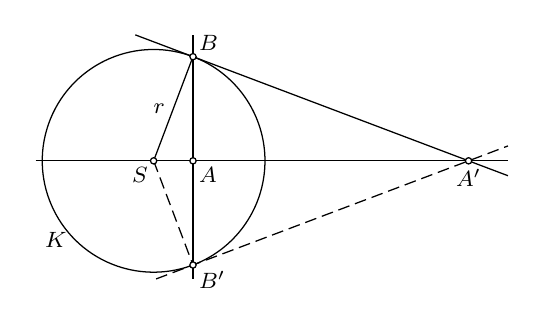
\begin{tikzpicture}
            % \clip (0,0) rectangle (14.000000,10.000000);
            {\footnotesize
            
            % Drawing circle k
            \draw [line width=0.016cm] (3.914214,2.500000) arc (0:67:1.414214 and 1.414214) -- (3.037213,3.808206);%
            \draw [line width=0.016cm] (2.962387,3.836487) -- (2.960423,3.837165) arc (71:289:1.414214 and 1.414214) -- (2.962387,1.163513);%
            \draw [line width=0.016cm] (3.037212,1.191794) -- (3.052577,1.198209) arc (293:359:1.414214 and 1.414214) -- (3.914214,2.500000);%
            
            % Drawing line s
            \draw [line width=0.016cm] (1.000000,2.500000) -- (2.460000,2.500000);%
            \draw [line width=0.016cm] (2.540000,2.500000) -- (2.960000,2.500000);%
            \draw [line width=0.016cm] (3.040000,2.500000) -- (6.460000,2.500000);%
            \draw [line width=0.016cm] (6.540000,2.500000) -- (7.000000,2.500000);%
            
            % Drawing segment S B
            \draw [line width=0.016cm] (2.514142,2.537417) -- (2.985858,3.785459);%
            
            % Drawing line x
            \draw [line width=0.016cm] (2.266798,4.100000) -- (2.962583,3.837018);%
            \draw [line width=0.016cm] (3.037417,3.808734) -- (6.462583,2.514142);%
            \draw [line width=0.016cm] (6.537417,2.485858) -- (7.000000,2.311018);%
            
            % Drawing line t
            \draw [line width=0.016cm] (3.000000,1.000000) -- (3.000000,1.137124);%
            \draw [line width=0.016cm] (3.000000,1.217124) -- (3.000000,2.460000);%
            \draw [line width=0.016cm] (3.000000,2.540000) -- (3.000000,3.782876);%
            \draw [line width=0.016cm] (3.000000,3.862876) -- (3.000000,4.100000);%
            
            % Drawing segment S B'
            \draw [line width=0.016cm] (2.514142,2.462583) -- (2.553033,2.359688);%
            \draw [line width=0.016cm] (2.579550,2.289532) -- (2.632583,2.149220);%
            \draw [line width=0.016cm] (2.659099,2.079064) -- (2.712132,1.938751);%
            \draw [line width=0.016cm] (2.738649,1.868595) -- (2.791682,1.728283);%
            \draw [line width=0.016cm] (2.818198,1.658127) -- (2.871231,1.517815);%
            \draw [line width=0.016cm] (2.897748,1.447659) -- (2.950781,1.307347);%
            \draw [line width=0.016cm] (2.977297,1.237191) -- (2.985858,1.214541);%
            
            % Drawing line y
            \draw [line width=0.016cm] (2.531373,1.000000) -- (2.671685,1.053033);%
            \draw [line width=0.016cm] (2.741841,1.079550) -- (2.882153,1.132583);%
            \draw [line width=0.016cm] (2.952309,1.159099) -- (2.962583,1.162982);%
            \draw [line width=0.016cm] (3.037417,1.191266) -- (3.092622,1.212132);%
            \draw [line width=0.016cm] (3.162778,1.238649) -- (3.303090,1.291682);%
            \draw [line width=0.016cm] (3.373246,1.318198) -- (3.513558,1.371231);%
            \draw [line width=0.016cm] (3.583714,1.397748) -- (3.724026,1.450781);%
            \draw [line width=0.016cm] (3.794182,1.477297) -- (3.934495,1.530330);%
            \draw [line width=0.016cm] (4.004651,1.556847) -- (4.144963,1.609880);%
            \draw [line width=0.016cm] (4.215119,1.636396) -- (4.355431,1.689429);%
            \draw [line width=0.016cm] (4.425587,1.715946) -- (4.565899,1.768979);%
            \draw [line width=0.016cm] (4.636055,1.795495) -- (4.776367,1.848528);%
            \draw [line width=0.016cm] (4.846524,1.875045) -- (4.986836,1.928078);%
            \draw [line width=0.016cm] (5.056992,1.954594) -- (5.197304,2.007627);%
            \draw [line width=0.016cm] (5.267460,2.034144) -- (5.407772,2.087177);%
            \draw [line width=0.016cm] (5.477928,2.113693) -- (5.618240,2.166726);%
            \draw [line width=0.016cm] (5.688396,2.193243) -- (5.828709,2.246276);%
            \draw [line width=0.016cm] (5.898865,2.272792) -- (6.039177,2.325825);%
            \draw [line width=0.016cm] (6.109333,2.352342) -- (6.249645,2.405375);%
            \draw [line width=0.016cm] (6.319801,2.431891) -- (6.460113,2.484924);%
            \draw [line width=0.016cm] (6.537417,2.514142) -- (6.670582,2.564474);%
            \draw [line width=0.016cm] (6.740738,2.590990) -- (6.881050,2.644023);%
            \draw [line width=0.016cm] (6.951206,2.670540) -- (7.000000,2.688982);%
            
            % Marking point S by circle
            \draw [line width=0.016cm] (2.500000,2.500000) circle (0.040000);%
            \draw (2.530000,2.530000) node [anchor=north east] { $S$ };%
            
            % Marking point K
            \draw (1.500000,1.500000) node [anchor=east] { $K$ };%
            
            % Marking point B by circle
            \draw [line width=0.016cm] (3.000000,3.822876) circle (0.040000);%
            \draw (2.970000,3.792876) node [anchor=south west] { $B$ };%
            
            % Marking point B' by circle
            \draw [line width=0.016cm] (3.000000,1.177124) circle (0.040000);%
            \draw (2.970000,1.207124) node [anchor=north west] { $B'$ };%
            
            % Marking point A' by circle
            \draw [line width=0.016cm] (6.500000,2.500000) circle (0.040000);%
            \draw (6.500000,2.500000) node [anchor=north] { $A'$ };%
            
            % Marking point A by circle
            \draw [line width=0.016cm] (3.000000,2.500000) circle (0.040000);%
            \draw (2.970000,2.530000) node [anchor=north west] { $A$ };%
            
            % Marking point r
            \draw (2.750000,3.161438) node [anchor=east] { $r$ };%
            }
        \end{tikzpicture}            
    \end{opomba}

    \begin{definicija}
        Naj bo $BB'$ tetiva krožnice $K$, ki ni njen premer.
        Potem je \textbf{pol} tetive $BB'$ presečišče tangent na krožnico $K$ v $B$ in $B'$.
    \end{definicija}

    \begin{trditev}[konstrukcija inverza]
        Naj bo $K$ krožnica s središčem $S$ in polmerom $r$.
        \begin{enumerate}
            \item Če $A\neq S$ leži znotraj krožnice $K$, naj bo premica $t$ pravokotnica na $\overleftrightarrow{AS}$ skozi točko A. Naj bosta $B$ in $B'$ presečišči $K$ in $t$. Potem je inverz $A'$ točke $A$ v $K$ enak polu tetive $BB'$.
            \item Če $A$ leži izven krožnice $K$, naj bo $\tilde{K}$ krožnica s premerom $|SA|$. Označimo z $B$ in $B'$ presečišči krožnic $K$ in $\tilde{K}$. Potem je $A'$ presečišče premic $\overleftrightarrow{SA}$ in $\overleftrightarrow{BB'}$.
        \end{enumerate}
    \end{trditev}

        \begin{dokaz}
            \\ (1)
            \\ 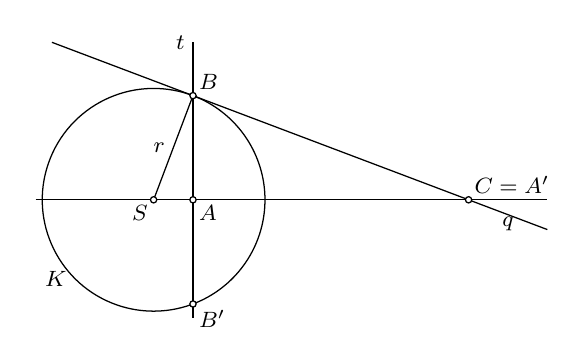
\begin{tikzpicture}
                    % \clip (0,0) rectangle (14.000000,10.000000);
                    {\footnotesize
                    
                    % Drawing circle k
                    \draw [line width=0.016cm] (3.914214,2.500000) arc (0:67:1.414214 and 1.414214) -- (3.037213,3.808206);%
                    \draw [line width=0.016cm] (2.962387,3.836487) -- (2.960423,3.837165) arc (71:289:1.414214 and 1.414214) -- (2.962387,1.163513);%
                    \draw [line width=0.016cm] (3.037212,1.191794) -- (3.052577,1.198209) arc (293:359:1.414214 and 1.414214) -- (3.914214,2.500000);%
                    
                    % Drawing line s
                    \draw [line width=0.016cm] (1.000000,2.500000) -- (2.460000,2.500000);%
                    \draw [line width=0.016cm] (2.540000,2.500000) -- (2.960000,2.500000);%
                    \draw [line width=0.016cm] (3.040000,2.500000) -- (6.460000,2.500000);%
                    \draw [line width=0.016cm] (6.540000,2.500000) -- (7.500000,2.500000);%
                    
                    % Drawing segment S B
                    \draw [line width=0.016cm] (2.514142,2.537417) -- (2.985858,3.785459);%
                    
                    % Drawing line x
                    \draw [line width=0.016cm] (1.208497,4.500000) -- (2.962583,3.837018);%
                    \draw [line width=0.016cm] (3.037417,3.808734) -- (6.462583,2.514142);%
                    \draw [line width=0.016cm] (6.537417,2.485858) -- (7.500000,2.122036);%
                    
                    % Drawing line T
                    \draw [line width=0.016cm] (3.000000,1.000000) -- (3.000000,1.137124);%
                    \draw [line width=0.016cm] (3.000000,1.217124) -- (3.000000,2.460000);%
                    \draw [line width=0.016cm] (3.000000,2.540000) -- (3.000000,3.782876);%
                    \draw [line width=0.016cm] (3.000000,3.862876) -- (3.000000,4.500000);%
                    
                    % Marking point t
                    \draw (3.000000,4.500000) node [anchor=east] { $t$ };%
                    
                    % Marking point S by circle
                    \draw [line width=0.016cm] (2.500000,2.500000) circle (0.040000);%
                    \draw (2.530000,2.530000) node [anchor=north east] { $S$ };%
                    
                    % Marking point K
                    \draw (1.500000,1.500000) node [anchor=east] { $K$ };%
                    
                    % Marking point B by circle
                    \draw [line width=0.016cm] (3.000000,3.822876) circle (0.040000);%
                    \draw (2.970000,3.792876) node [anchor=south west] { $B$ };%
                    
                    % Marking point B' by circle
                    \draw [line width=0.016cm] (3.000000,1.177124) circle (0.040000);%
                    \draw (2.970000,1.207124) node [anchor=north west] { $B'$ };%
                    
                    % Marking point A'=C by circle
                    \draw [line width=0.016cm] (6.500000,2.500000) circle (0.040000);%
                    \draw (6.470000,2.470000) node [anchor=south west] { $C=A'$ };%
                    
                    % Marking point A by circle
                    \draw [line width=0.016cm] (3.000000,2.500000) circle (0.040000);%
                    \draw (2.970000,2.530000) node [anchor=north west] { $A$ };%
                    
                    % Marking point r
                    \draw (2.750000,3.161438) node [anchor=east] { $r$ };%
                    
                    % Marking point q
                    \draw (7.000000,2.000000) node [anchor=south] { $q$ };%
                    }
                \end{tikzpicture}                
            \\ Naj bo $q\perp \overleftrightarrow{SB}$ skozi $B$ in $C=\overleftrightarrow{SA}\cap q$. Zaradi kotov sledi, da sta trikotnika $\triangle SAB$ in $\triangle SBC$ podobna (skupen kot $\angle S$, prava kota $\angle A$ in $\angle B$). 
            $\Rightarrow \frac{|SA|}{|SB|}=\frac{|SB|}{|SC|} \Rightarrow |SA|\cdot|SC|=|SB|^2=r^2 \Rightarrow$ $C$  je inverz točke $A$ v $K$ $\Rightarrow$ $C=A'$
            ($C$ je pol daljice $BB'$, saj simetrična konstrukcija pod $\overleftrightarrow{AS}$ da isto točko $C$.)
            \\ (2)
            \\ 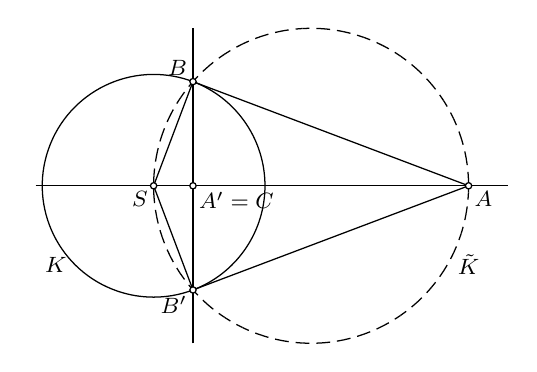
\begin{tikzpicture}
                    % \clip (0,0) rectangle (14.000000,10.000000);
                    {\footnotesize
                    
                    % Drawing circle k
                    \draw [line width=0.016cm] (3.914214,3.500000) arc (0:67:1.414214 and 1.414214) -- (3.037213,4.808206);%
                    \draw [line width=0.016cm] (2.962387,4.836487) -- (2.960423,4.837165) arc (71:289:1.414214 and 1.414214) -- (2.962387,2.163513);%
                    \draw [line width=0.016cm] (3.037212,2.191794) -- (3.052577,2.198209) arc (293:360:1.414214 and 1.414214) --(3.914214,3.500000) arc (0:0:1.414214 and 1.414214);%
                    
                    % Drawing line s
                    \draw [line width=0.016cm] (1.000000,3.500000) -- (2.460000,3.500000);%
                    \draw [line width=0.016cm] (2.540000,3.500000) -- (2.960000,3.500000);%
                    \draw [line width=0.016cm] (3.040000,3.500000) -- (6.460000,3.500000);%
                    \draw [line width=0.016cm] (6.540000,3.500000) -- (7.000000,3.500000);%
                    
                    % Drawing segment S B
                    \draw [line width=0.016cm] (2.514142,3.537417) -- (2.985858,4.785459);%
                    
                    % Drawing segment B A
                    \draw [line width=0.016cm] (3.037417,4.808734) -- (6.462583,3.514142);%
                    
                    % Drawing line t
                    \draw [line width=0.016cm] (3.000000,1.500000) -- (3.000000,2.137124);%
                    \draw [line width=0.016cm] (3.000000,2.217124) -- (3.000000,3.460000);%
                    \draw [line width=0.016cm] (3.000000,3.540000) -- (3.000000,4.782876);%
                    \draw [line width=0.016cm] (3.000000,4.862876) -- (3.000000,5.500000);%
                    
                    % Drawing circle k'
                    \draw [line width=0.016cm] (6.499600,3.539998) -- (6.498782,3.569799) arc (2:2:2.000000 and 2.000000) -- (6.498070,3.587848);%
                    \draw [line width=0.016cm] (6.498070,3.587848) -- (6.497259,3.604672) arc (3:5:2.000000 and 2.000000) -- (6.492283,3.675527);%
                    \draw [line width=0.016cm] (6.482650,3.762867) -- (6.480536,3.778346) arc (8:10:2.000000 and 2.000000) -- (6.469190,3.849700);%
                    \draw [line width=0.016cm] (6.469190,3.849700) -- (6.463254,3.881618) arc (11:12:2.000000 and 2.000000) -- (6.451929,3.935858);%
                    \draw [line width=0.016cm] (6.430901,4.021174) -- (6.422523,4.051275) arc (16:17:2.000000 and 2.000000) -- (6.406145,4.105484);%
                    \draw [line width=0.016cm] (6.406145,4.105484) -- (6.402113,4.118034) arc (18:20:2.000000 and 2.000000) -- (6.377710,4.188626);%
                    \draw [line width=0.016cm] (6.345650,4.270438) -- (6.341010,4.281462) arc (23:25:2.000000 and 2.000000) -- (6.310028,4.350763);%
                    \draw [line width=0.016cm] (6.310028,4.350763) -- (6.297588,4.376742) arc (26:27:2.000000 and 2.000000) -- (6.270912,4.429446);%
                    \draw [line width=0.016cm] (6.228378,4.506335) -- (6.214335,4.530076) arc (31:32:2.000000 and 2.000000) -- (6.182507,4.581282);%
                    \draw [line width=0.016cm] (6.182507,4.581282) -- (6.177341,4.589278) arc (33:35:2.000000 and 2.000000) -- (6.133389,4.654141);%
                    \draw [line width=0.016cm] (6.081118,4.724772) -- (6.076022,4.731323) arc (38:40:2.000000 and 2.000000) -- (6.025794,4.793040);%
                    \draw [line width=0.016cm] (6.025794,4.793040) -- (6.009419,4.812118) arc (41:42:2.000000 and 2.000000) -- (5.967526,4.858811);%
                    \draw [line width=0.016cm] (5.906425,4.921959) -- (5.889317,4.938680) arc (46:47:2.000000 and 2.000000) -- (5.842609,4.982363);%
                    \draw [line width=0.016cm] (5.842609,4.982363) -- (5.838261,4.986290) arc (48:50:2.000000 and 2.000000) -- (5.776202,5.039906);%
                    \draw [line width=0.016cm] (5.707331,5.094475) -- (5.703630,5.097271) arc (53:55:2.000000 and 2.000000) -- (5.636130,5.145968);%
                    \draw [line width=0.016cm] (5.636130,5.145968) -- (5.618386,5.158075) arc (56:57:2.000000 and 2.000000) -- (5.562735,5.194283);%
                    \draw [line width=0.016cm] (5.487289,5.239327) -- (5.469619,5.249239) arc (61:62:2.000000 and 2.000000) -- (5.409938,5.281015);%
                    \draw [line width=0.016cm] (5.409938,5.281015) -- (5.407981,5.282013) arc (63:65:2.000000 and 2.000000) -- (5.330830,5.319264);%
                    \draw [line width=0.016cm] (5.250119,5.354002) -- (5.249213,5.354368) arc (68:70:2.000000 and 2.000000) -- (5.167959,5.385161);%
                    \draw [line width=0.016cm] (5.167959,5.385161) -- (5.151136,5.391037) arc (71:73:2.000000 and 2.000000) -- (5.084510,5.412681);%
                    \draw [line width=0.016cm] (4.999933,5.436509) -- (4.983844,5.440591) arc (76:78:2.000000 and 2.000000) -- (4.914391,5.456599);%
                    \draw [line width=0.016cm] (4.914391,5.456599) -- (4.881618,5.463254) arc (79:80:2.000000 and 2.000000) -- (4.828049,5.472913);%
                    \draw [line width=0.016cm] (4.741074,5.485418) -- (4.709057,5.489044) arc (84:85:2.000000 and 2.000000) -- (4.653633,5.494091);%
                    \draw [line width=0.016cm] (4.653633,5.494091) -- (4.639513,5.495128) arc (86:88:2.000000 and 2.000000) -- (4.565896,5.498914);%
                    \draw [line width=0.016cm] (4.478031,5.499879) -- (4.465095,5.499695) arc (91:93:2.000000 and 2.000000) -- (4.390209,5.496984);%
                    \draw [line width=0.016cm] (4.390209,5.496984) -- (4.360487,5.495128) arc (94:95:2.000000 and 2.000000) -- (4.302599,5.490234);%
                    \draw [line width=0.016cm] (4.215370,5.479643) -- (4.187131,5.475377) arc (99:100:2.000000 and 2.000000) -- (4.128691,5.465230);%
                    \draw [line width=0.016cm] (4.128691,5.465230) -- (4.118382,5.463254) arc (101:103:2.000000 and 2.000000) -- (4.042728,5.447024);%
                    \draw [line width=0.016cm] (3.957648,5.425060) -- (3.948725,5.422523) arc (106:108:2.000000 and 2.000000) -- (3.873615,5.399379);%
                    \draw [line width=0.016cm] (3.873615,5.399379) -- (3.848864,5.391037) arc (109:110:2.000000 and 2.000000) -- (3.790790,5.370033);%
                    \draw [line width=0.016cm] (3.709335,5.337076) -- (3.686527,5.327091) arc (114:115:2.000000 and 2.000000) -- (3.629406,5.300574);%
                    \draw [line width=0.016cm] (3.629406,5.300574) -- (3.623258,5.297588) arc (116:118:2.000000 and 2.000000) -- (3.551158,5.260596);%
                    \draw [line width=0.016cm] (3.474741,5.217220) -- (3.469924,5.214335) arc (121:123:2.000000 and 2.000000) -- (3.400302,5.170528);%
                    \draw [line width=0.016cm] (3.400302,5.170528) -- (3.381614,5.158075) arc (124:125:2.000000 and 2.000000) -- (3.327987,5.120613);%
                    \draw [line width=0.016cm] (3.257934,5.067569) -- (3.241359,5.054292) arc (129:130:2.000000 and 2.000000) -- (3.190279,5.011499);%
                    \draw [line width=0.016cm] (3.190279,5.011499) -- (3.187882,5.009419) arc (131:133:2.000000 and 2.000000) -- (3.125151,4.952512);%
                    \draw [line width=0.016cm] (3.062678,4.890721) -- (3.061321,4.889317) arc (136:137:2.000000 and 2.000000) -- (3.026756,4.852610);%
                    \draw [line width=0.016cm] (2.973844,4.792613) -- (2.967911,4.785575) arc (140:140:2.000000 and 2.000000) -- (2.946169,4.759210);%
                    \draw [line width=0.016cm] (2.892359,4.689744) -- (2.881966,4.675571) arc (144:146:2.000000 and 2.000000) -- (2.841652,4.617981);%
                    \draw [line width=0.016cm] (2.841652,4.617981) -- (2.822659,4.589278) arc (147:148:2.000000 and 2.000000) -- (2.794146,4.544061);%
                    \draw [line width=0.016cm] (2.749933,4.468125) -- (2.734105,4.438943) arc (152:153:2.000000 and 2.000000) -- (2.709098,4.390320);%
                    \draw [line width=0.016cm] (2.709098,4.390320) -- (2.702412,4.376743) arc (154:156:2.000000 and 2.000000) -- (2.671720,4.310797);%
                    \draw [line width=0.016cm] (2.637871,4.229708) -- (2.632839,4.216736) arc (159:161:2.000000 and 2.000000) -- (2.607616,4.147212);%
                    \draw [line width=0.016cm] (2.607616,4.147212) -- (2.597887,4.118034) arc (162:163:2.000000 and 2.000000) -- (2.581014,4.063465);%
                    \draw [line width=0.016cm] (2.558116,3.978632) -- (2.551260,3.949902) arc (167:168:2.000000 and 2.000000) -- (2.538967,3.892874);%
                    \draw [line width=0.016cm] (2.538967,3.892874) -- (2.536746,3.881618) arc (169:171:2.000000 and 2.000000) -- (2.523603,3.806358);%
                    \draw [line width=0.016cm] (2.512054,3.719251) -- (2.510956,3.709057) arc (174:176:2.000000 and 2.000000) -- (2.504342,3.631720);%
                    \draw [line width=0.016cm] (2.504342,3.631720) -- (2.502741,3.604672) arc (177:178:2.000000 and 2.000000) -- (2.500483,3.543935);%
                    \draw [line width=0.016cm] (2.500483,3.456066) -- (2.501218,3.430201) arc (182:183:2.000000 and 2.000000) -- (2.504342,3.368281);%
                    \draw [line width=0.016cm] (2.504342,3.368281) -- (2.504872,3.360487) arc (184:186:2.000000 and 2.000000) -- (2.512054,3.280751);%
                    \draw [line width=0.016cm] (2.523603,3.193643) -- (2.524623,3.187131) arc (189:191:2.000000 and 2.000000) -- (2.538967,3.107127);%
                    \draw [line width=0.016cm] (2.538967,3.107127) -- (2.543705,3.084177) arc (192:193:2.000000 and 2.000000) -- (2.558116,3.021370);%
                    \draw [line width=0.016cm] (2.581014,2.936536) -- (2.587390,2.915257) arc (197:198:2.000000 and 2.000000) -- (2.607616,2.852790);%
                    \draw [line width=0.016cm] (2.607616,2.852790) -- (2.608963,2.848864) arc (199:201:2.000000 and 2.000000) -- (2.637870,2.770293);%
                    \draw [line width=0.016cm] (2.671719,2.689204) -- (2.672909,2.686527) arc (204:206:2.000000 and 2.000000) -- (2.709097,2.609681);%
                    \draw [line width=0.016cm] (2.709097,2.609681) -- (2.717987,2.592019) arc (207:208:2.000000 and 2.000000) -- (2.749932,2.531876);%
                    \draw [line width=0.016cm] (2.794145,2.455940) -- (2.803904,2.440162) arc (212:213:2.000000 and 2.000000) -- (2.841651,2.382020);%
                    \draw [line width=0.016cm] (2.841651,2.382020) -- (2.841925,2.381614) arc (214:216:2.000000 and 2.000000) -- (2.892358,2.310257);%
                    \draw [line width=0.016cm] (2.946168,2.240791) -- (2.967911,2.214425) arc (220:220:2.000000 and 2.000000) -- (2.973843,2.207388);%
                    \draw [line width=0.016cm] (3.026756,2.147391) -- (3.037292,2.136004) arc (223:224:2.000000 and 2.000000) -- (3.062677,2.109280);%
                    \draw [line width=0.016cm] (3.125150,2.047489) -- (3.136003,2.037293) arc (227:229:2.000000 and 2.000000) -- (3.190278,1.988502);%
                    \draw [line width=0.016cm] (3.190278,1.988502) -- (3.214424,1.967911) arc (230:231:2.000000 and 2.000000) -- (3.257933,1.932432);%
                    \draw [line width=0.016cm] (3.327986,1.879388) -- (3.352847,1.861696) arc (235:236:2.000000 and 2.000000) -- (3.400301,1.829472);%
                    \draw [line width=0.016cm] (3.400301,1.829472) -- (3.410722,1.822659) arc (237:239:2.000000 and 2.000000) -- (3.474739,1.782781);%
                    \draw [line width=0.016cm] (3.551156,1.739405) -- (3.561057,1.734105) arc (242:244:2.000000 and 2.000000) -- (3.629405,1.699427);%
                    \draw [line width=0.016cm] (3.629405,1.699427) -- (3.654763,1.687385) arc (245:246:2.000000 and 2.000000) -- (3.709334,1.662924);%
                    \draw [line width=0.016cm] (3.790789,1.629968) -- (3.815959,1.620615) arc (250:251:2.000000 and 2.000000) -- (3.873613,1.600621);%
                    \draw [line width=0.016cm] (3.873613,1.600621) -- (3.881966,1.597887) arc (252:254:2.000000 and 2.000000) -- (3.957647,1.574941);%
                    \draw [line width=0.016cm] (4.042727,1.552976) -- (4.050097,1.551260) arc (257:259:2.000000 and 2.000000) -- (4.128690,1.534770);%
                    \draw [line width=0.016cm] (4.128690,1.534770) -- (4.152703,1.530385) arc (260:261:2.000000 and 2.000000) -- (4.215369,1.520357);%
                    \draw [line width=0.016cm] (4.302598,1.509766) -- (4.325688,1.507611) arc (265:266:2.000000 and 2.000000) -- (4.390208,1.503016);%
                    \draw [line width=0.016cm] (4.390208,1.503016) -- (4.395328,1.502741) arc (267:269:2.000000 and 2.000000) -- (4.478030,1.500121);%
                    \draw [line width=0.016cm] (4.565895,1.501086) -- (4.569799,1.501218) arc (272:274:2.000000 and 2.000000) -- (4.653632,1.505909);%
                    \draw [line width=0.016cm] (4.653632,1.505909) -- (4.674311,1.507611) arc (275:276:2.000000 and 2.000000) -- (4.741072,1.514582);%
                    \draw [line width=0.016cm] (4.828048,1.527087) -- (4.847296,1.530384) arc (280:281:2.000000 and 2.000000) -- (4.914390,1.543401);%
                    \draw [line width=0.016cm] (4.914390,1.543401) -- (4.915823,1.543705) arc (282:284:2.000000 and 2.000000) -- (4.999932,1.563491);%
                    \draw [line width=0.016cm] (5.084509,1.587319) -- (5.084743,1.587390) arc (287:289:2.000000 and 2.000000) -- (5.167958,1.614839);%
                    \draw [line width=0.016cm] (5.167958,1.614839) -- (5.184040,1.620615) arc (290:292:2.000000 and 2.000000) -- (5.250117,1.645998);%
                    \draw [line width=0.016cm] (5.330829,1.680736) -- (5.345236,1.687384) arc (295:297:2.000000 and 2.000000) -- (5.409937,1.718985);%
                    \draw [line width=0.016cm] (5.409937,1.718985) -- (5.438943,1.734105) arc (298:299:2.000000 and 2.000000) -- (5.487288,1.760672);%
                    \draw [line width=0.016cm] (5.562734,1.805717) -- (5.589278,1.822659) arc (303:304:2.000000 and 2.000000) -- (5.636129,1.854032);%
                    \draw [line width=0.016cm] (5.636129,1.854032) -- (5.647152,1.861696) arc (305:307:2.000000 and 2.000000) -- (5.707330,1.905524);%
                    \draw [line width=0.016cm] (5.776201,1.960094) -- (5.785575,1.967911) arc (310:312:2.000000 and 2.000000) -- (5.842608,2.017636);%
                    \draw [line width=0.016cm] (5.842608,2.017636) -- (5.863996,2.037292) arc (313:314:2.000000 and 2.000000) -- (5.906424,2.078040);%
                    \draw [line width=0.016cm] (5.967525,2.141188) -- (5.986289,2.161738) arc (318:319:2.000000 and 2.000000) -- (6.025794,2.206960);%
                    \draw [line width=0.016cm] (6.025794,2.206960) -- (6.032089,2.214424) arc (320:322:2.000000 and 2.000000) -- (6.081117,2.275227);%
                    \draw [line width=0.016cm] (6.133388,2.345858) -- (6.138304,2.352847) arc (325:327:2.000000 and 2.000000) -- (6.182506,2.418717);%
                    \draw [line width=0.016cm] (6.182506,2.418717) -- (6.196096,2.440161) arc (328:329:2.000000 and 2.000000) -- (6.228377,2.493664);%
                    \draw [line width=0.016cm] (6.270912,2.570553) -- (6.282013,2.592018) arc (333:334:2.000000 and 2.000000) -- (6.310028,2.649236);%
                    \draw [line width=0.016cm] (6.310028,2.649236) -- (6.312615,2.654763) arc (335:337:2.000000 and 2.000000) -- (6.345650,2.729561);%
                    \draw [line width=0.016cm] (6.377709,2.811373) -- (6.379385,2.815959) arc (340:342:2.000000 and 2.000000) -- (6.406145,2.894515);%
                    \draw [line width=0.016cm] (6.406145,2.894515) -- (6.412609,2.915256) arc (343:344:2.000000 and 2.000000) -- (6.430900,2.978825);%
                    \draw [line width=0.016cm] (6.451929,3.064141) -- (6.456295,3.084176) arc (348:349:2.000000 and 2.000000) -- (6.469190,3.150299);%
                    \draw [line width=0.016cm] (6.469190,3.150299) -- (6.469615,3.152703) arc (350:352:2.000000 and 2.000000) -- (6.482650,3.237131);%
                    \draw [line width=0.016cm] (6.492283,3.324471) -- (6.492389,3.325688) arc (355:357:2.000000 and 2.000000) -- (6.498070,3.412150);%
                    \draw [line width=0.016cm] (6.498070,3.412150) -- (6.498782,3.430200) arc (358:358:2.000000 and 2.000000) -- (6.499600,3.460001);%
                    
                    % Drawing segment S B'
                    \draw [line width=0.016cm] (2.514142,3.462583) -- (2.985858,2.214541);%
                    
                    % Drawing segment B' A
                    \draw [line width=0.016cm] (3.037417,2.191266) -- (6.462583,3.485858);%
                    
                    % Marking point S by circle
                    \draw [line width=0.016cm] (2.500000,3.500000) circle (0.040000);%
                    \draw (2.530000,3.530000) node [anchor=north east] { $S$ };%
                    
                    % Marking point K
                    \draw (1.500000,2.500000) node [anchor=east] { $K$ };%
                    
                    % Marking point B by circle
                    \draw [line width=0.016cm] (3.000000,4.822876) circle (0.040000);%
                    \draw (3.030000,4.792876) node [anchor=south east] { $B$ };%
                    
                    % Marking point B' by circle
                    \draw [line width=0.016cm] (3.000000,2.177124) circle (0.040000);%
                    \draw (3.030000,2.207124) node [anchor=north east] { $B'$ };%
                    
                    % Marking point A by circle
                    \draw [line width=0.016cm] (6.500000,3.500000) circle (0.040000);%
                    \draw (6.470000,3.530000) node [anchor=north west] { $A$ };%
                    
                    % Marking point A'=C by circle
                    \draw [line width=0.016cm] (3.000000,3.500000) circle (0.040000);%
                    \draw (2.970000,3.530000) node [anchor=north west] { $A'=C$ };%
                    
                    % Marking point \tilde{K}
                    \draw (6.500000,2.500000) node  { $\tilde{K}$ };%
                    }
                \end{tikzpicture}                
            \\ Ker je trikotnik $\triangle SAB$ včrtan v polkrog, je pravokoten, $|\angle B|=\frac{\pi}{2}$. Trikotnika $\triangle SAB$ in $\triangle SAB'$ sta skladna, saj sta pravokotna, imata skupno hipotenuzo in skladni kateti $SB\cong SB'$. Sledi: $\angle ASB\cong \angle ASB'$. Po kriteriju SKS velja: $\triangle BSC\cong\triangle B'SC \Rightarrow \angle SCB\cong\angle SCB'\cong pravi~kot$.
             $\Rightarrow \triangle SCB\sim\triangle SBA \rightarrow \frac{|SC|}{|SB|}=\frac{|SB|}{|SA|} \Rightarrow |SA|\cdot|SC|=|SB|^2=r^2 \Rightarrow C=A'$.
        \end{dokaz}

    \begin{trditev}
        Naj bo $K$ krožnica s središčem $S$ in polmerom $r$ ter $A\neq S, A\notin K$ in naj bo $\tilde{K}$ krožnica skozi $A$. 
        Velja: $\tilde{K}\perp K\Leftrightarrow A'\in \tilde{K}$.
    \end{trditev}

        \begin{dokaz}
            \\ 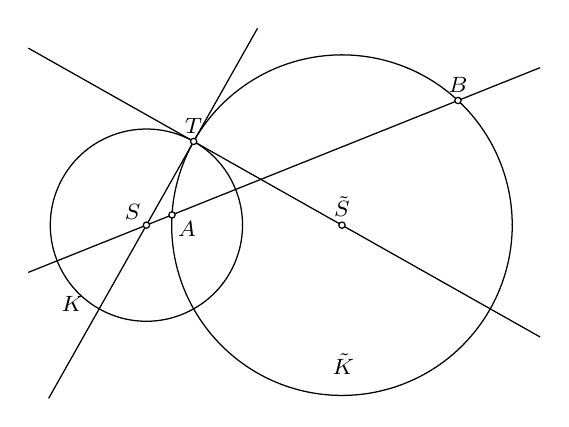
\begin{tikzpicture}
                    % \clip (0,0) rectangle (14.000000,10.000000);
                    {\footnotesize
                    
                    % Drawing circle k
                    \draw [line width=0.016cm] (3.720656,3.500000) arc (0:58:1.220656 and 1.220656) -- (3.134507,4.542785);%
                    \draw [line width=0.016cm] (3.064848,4.582103) -- (3.054166,4.587612) arc (63:360:1.220656 and 1.220656) --(3.720656,3.500000) arc (0:0:1.220656 and 1.220656);%
                    
                    % Drawing circle k'
                    \draw [line width=0.016cm] (7.145958,3.500000) arc (0:45:2.162624 and 2.162624) -- (6.486021,5.055273);%
                    \draw [line width=0.016cm] (6.427472,5.109785) -- (6.402143,5.132153) arc (49:149:2.162624 and 2.162624) -- (3.119983,4.597665);%
                    \draw [line width=0.016cm] (3.080661,4.528000) -- (3.073849,4.515291) arc (152:175:2.162624 and 2.162624) -- (2.827381,3.669748);%
                    \draw [line width=0.016cm] (2.822578,3.589896) -- (2.822026,3.575475) arc (178:360:2.162624 and 2.162624) --(7.145958,3.500000) arc (0:0:2.162624 and 2.162624);%
                    
                    % Drawing line R
                    \draw [line width=0.016cm] (1.258248,1.300000) -- (2.480338,3.465166);%
                    \draw [line width=0.016cm] (2.519662,3.534834) -- (3.080338,4.528180);%
                    \draw [line width=0.016cm] (3.119662,4.597849) -- (3.911081,6.000000);%
                    
                    % Drawing line x
                    \draw [line width=0.016cm] (1.000000,5.748323) -- (3.065166,4.582676);%
                    \draw [line width=0.016cm] (3.134834,4.543353) -- (4.948499,3.519662);%
                    \draw [line width=0.016cm] (5.018168,3.480338) -- (7.500000,2.079511);%
                    
                    % Drawing line u
                    \draw [line width=0.016cm] (1.000000,2.900000) -- (2.462861,3.485144);%
                    \draw [line width=0.016cm] (2.537139,3.514856) -- (2.787471,3.614989);%
                    \draw [line width=0.016cm] (2.861749,3.644700) -- (6.419860,5.067944);%
                    \draw [line width=0.016cm] (6.494138,5.097655) -- (7.500000,5.500000);%
                    
                    % Marking point S by circle
                    \draw [line width=0.016cm] (2.500000,3.500000) circle (0.040000);%
                    \draw (2.530000,3.470000) node [anchor=south east] { $S$ };%
                    
                    % Marking point K
                    \draw (1.800000,2.500000) node [anchor=east] { $K$ };%
                    
                    % Marking point T by circle
                    \draw [line width=0.016cm] (3.100000,4.563015) circle (0.040000);%
                    \draw (3.100000,4.563015) node [anchor=south] { $T$ };%
                    
                    % Marking point \tilde{S} by circle
                    \draw [line width=0.016cm] (4.983333,3.500000) circle (0.040000);%
                    \draw (4.983333,3.500000) node [anchor=south] { $\tilde{S}$ };%
                    
                    % Marking point A by circle
                    \draw [line width=0.016cm] (2.824610,3.629844) circle (0.040000);%
                    \draw (2.794610,3.659844) node [anchor=north west] { $A$ };%
                    
                    % Marking point B by circle
                    \draw [line width=0.016cm] (6.456999,5.082800) circle (0.040000);%
                    \draw (6.456999,5.082800) node [anchor=south] { $B$ };%
                    
                    % Marking point \tilde{K}
                    \draw (5.000000,1.500000) node [anchor=south] { $\tilde{K}$ };%
                    }
                \end{tikzpicture}                
            \\ ($\Rightarrow$): Ker sta $K$ in $\tilde{K}$ pravokotni, za presečišče $T\in K\cap \tilde{K}$ velja: $\overleftrightarrow{ST}$ je tangenta na $\tilde{K}$ (polmera krožnic sta pravokotna v točki $T$). Potem je po potenci točke na krožnico: $|SA|\cdot |SB|=|ST|^2=r^2$. Od tod sledi: $B=A'$.
            \\ 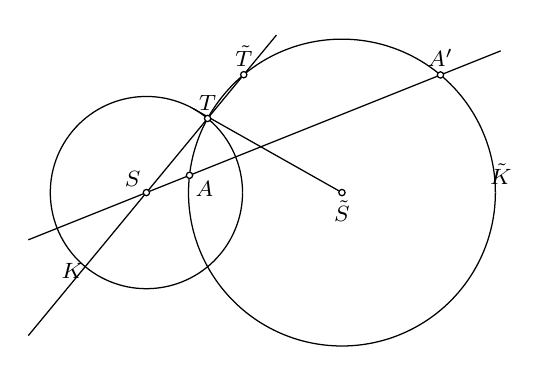
\begin{tikzpicture}
                    % \clip (0,0) rectangle (14.000000,10.000000);
                    {\footnotesize
                    
                    % Drawing circle k
                    \draw [line width=0.016cm] (3.720656,3.500000) arc (0:48:1.220656 and 1.220656) -- (3.307605,4.415300);%
                    \draw [line width=0.016cm] (3.245923,4.466229) -- (3.234609,4.474859) arc (53:359:1.220656 and 1.220656) -- (3.720656,3.500000);%
                    
                    % Drawing circle k'
                    \draw [line width=0.016cm] (6.931908,3.500000) arc (0:48:1.948575 and 1.948575) -- (6.264923,4.967812);%
                    \draw [line width=0.016cm] (6.203597,5.019178) -- (6.182996,5.035498) arc (52:128:1.948575 and 1.948575) -- (3.767183,5.022472);%
                    \draw [line width=0.016cm] (3.705718,4.971273) -- (3.704953,4.970608) arc (131:149:1.948575 and 1.948575) -- (3.296862,4.476094);%
                    \draw [line width=0.016cm] (3.258219,4.406050) -- (3.247140,4.384635) arc (153:172:1.948575 and 1.948575) -- (3.051985,3.758533);%
                    \draw [line width=0.016cm] (3.043001,3.679043) -- (3.042173,3.669830) arc (175:359:1.948575 and 1.948575) -- (6.931908,3.499999);%
                    
                    % Drawing line u
                    \draw [line width=0.016cm] (1.000000,2.900000) -- (2.462861,3.485144);%
                    \draw [line width=0.016cm] (2.537139,3.514856) -- (3.009946,3.703979);%
                    \draw [line width=0.016cm] (3.084224,3.733690) -- (6.197385,4.978954);%
                    \draw [line width=0.016cm] (6.271663,5.008665) -- (7.000000,5.300000);%
                    
                    % Drawing segment \tilde{S} U
                    \draw [line width=0.016cm] (4.948499,3.519662) -- (3.317172,4.440435);%
                    \draw [line width=0.016cm] (3.255800,4.475076) -- (3.100000,4.563015);%
                    
                    % Drawing line z
                    \draw [line width=0.016cm] (4.151346,5.500000) -- (3.761655,5.028033);%
                    \draw [line width=0.016cm] (3.710720,4.966343) -- (3.302649,4.472115);%
                    \draw [line width=0.016cm] (3.251714,4.410425) -- (2.525468,3.530845);%
                    \draw [line width=0.016cm] (2.474532,3.469155) -- (1.000000,1.683300);%
                    
                    % Marking point S by circle
                    \draw [line width=0.016cm] (2.500000,3.500000) circle (0.040000);%
                    \draw (2.530000,3.470000) node [anchor=south east] { $S$ };%
                    
                    % Marking point K
                    \draw (1.800000,2.500000) node [anchor=east] { $K$ };%
                    
                    % Marking point \tilde{S} by circle
                    \draw [line width=0.016cm] (4.983333,3.500000) circle (0.040000);%
                    \draw (4.983333,3.500000) node [anchor=north] { $\tilde{S}$ };%
                    
                    % Marking point A by circle
                    \draw [line width=0.016cm] (3.047085,3.718834) circle (0.040000);%
                    \draw (3.017085,3.748834) node [anchor=north west] { $A$ };%
                    
                    % Marking point A' by circle
                    \draw [line width=0.016cm] (6.234524,4.993810) circle (0.040000);%
                    \draw (6.234524,4.993810) node [anchor=south] { $A'$ };%
                    
                    % Marking point \tilde{K}
                    \draw (7.000000,3.500000) node [anchor=south] { $\tilde{K}$ };%
                    
                    % Marking point T by circle
                    \draw [line width=0.016cm] (3.277181,4.441270) circle (0.040000);%
                    \draw (3.277181,4.441270) node [anchor=south] { $T$ };%
                    
                    % Marking point \tilde{T} by circle
                    \draw [line width=0.016cm] (3.736188,4.997188) circle (0.040000);%
                    \draw (3.736188,4.997188) node [anchor=south] { $\tilde{T}$ };%
                    }
                \end{tikzpicture}
            \\ ($\Leftarrow$): Za pravokotnost krožnic moramo dokazati pravokotnost polmerov oziroma to, da je $\overleftrightarrow{ST}$ tangenta na krožnico $\tilde{K}$. Velja: $r^2=|SA|\cdot |SA'|=|ST|\cdot |S\tilde{T}|$. Če $\overleftrightarrow{ST}$ ni tangenta na $\tilde{K}$, potem jo seka še v točki $\tilde{T}$. Ker je $|ST|=r$, sledi: $|S\tilde{T}|=r$. Od tod sledi $T=\tilde{T}$, kar pa nas privede v protislovje ($T\neq \tilde{T}$).
        \end{dokaz}

    \begin{posledica}
        $\tilde{K}\perp K \Leftrightarrow$ inverzija v $K$ slika $\tilde{K}$ nazaj vase.
    \end{posledica}

\subsection{Premice in krožnice pri inverziji}

    Naj bo $K$ krožnica s središčem v $S$ in polmerom $r$ krožnica inverzije.
    Zanimajo nas slike premic in krožnic pri inverziji v $K$. Pri tem ločimo več primerov:

    \begin{enumerate}
        \item \uline{premica $p$ gre skozi $S$}:
            \\ 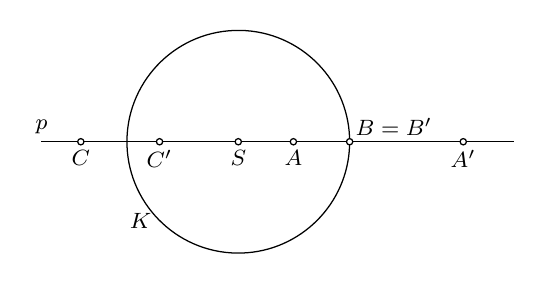
\begin{tikzpicture}
                % \clip (0,0) rectangle (14.000000,10.000000);
                {\footnotesize
                
                % Drawing circle k
                \draw [line width=0.016cm] (5.913648,2.539996) -- (5.913352,2.549355) arc (2:358:1.414214 and 1.414214) -- (5.913648,2.460004);%
                
                % Drawing line s
                \draw [line width=0.016cm] (2.000000,2.500000) -- (2.460000,2.500000);%
                \draw [line width=0.016cm] (2.540000,2.500000) -- (3.460000,2.500000);%
                \draw [line width=0.016cm] (3.540000,2.500000) -- (4.460000,2.500000);%
                \draw [line width=0.016cm] (4.540000,2.500000) -- (5.160000,2.500000);%
                \draw [line width=0.016cm] (5.240000,2.500000) -- (5.874214,2.500000);%
                \draw [line width=0.016cm] (5.954214,2.500000) -- (7.317143,2.500000);%
                \draw [line width=0.016cm] (7.397143,2.500000) -- (8.000000,2.500000);%
                
                % Marking point S by circle
                \draw [line width=0.016cm] (4.500000,2.500000) circle (0.040000);%
                \draw (4.500000,2.500000) node [anchor=north] { $S$ };%
                
                % Marking point K
                \draw (3.500000,1.500000) node [anchor=east] { $K$ };%

                % Marking point p
                \draw (2.00000,2.500000) node [anchor=south] { $p$ };%

                % Marking point A' by circle
                \draw [line width=0.016cm] (7.357143,2.500000) circle (0.040000);%
                \draw (7.357143,2.500000) node [anchor=north] { $A'$ };%
                
                % Marking point A by circle
                \draw [line width=0.016cm] (5.200000,2.500000) circle (0.040000);%
                \draw (5.200000,2.500000) node [anchor=north] { $A$ };%
                
                % Marking point C by circle
                \draw [line width=0.016cm] (2.500000,2.500000) circle (0.040000);%
                \draw (2.500000,2.500000) node [anchor=north] { $C$ };%
                
                % Marking point C' by circle
                \draw [line width=0.016cm] (3.500000,2.500000) circle (0.040000);%
                \draw (3.500000,2.500000) node [anchor=north] { $C'$ };%
                
                % Marking point B=B' by circle
                \draw [line width=0.016cm] (5.914214,2.500000) circle (0.040000);%
                \draw (5.884214,2.470000) node [anchor=south west] { $B=B'$ };%
                }
                \end{tikzpicture}
            \\ Inverzija v $K$ ($inv_K$) slika $p\backslash \{S\}$ nazaj vase.
        \item \uline{premica $p$ ne vsebuje $S$}:
            \\ 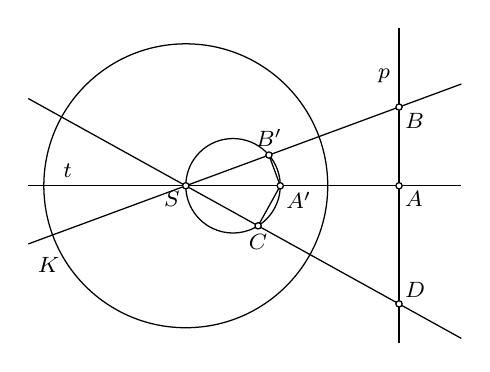
\begin{tikzpicture}
                % \clip (0,0) rectangle (14.000000,10.000000);
                {\footnotesize
                
                % Drawing circle k
                \draw [line width=0.016cm] (4.500000,3.500000) circle (1.802776);%
                
                % Drawing line s
                \draw [line width=0.016cm] (2.500000,3.500000) -- (4.460000,3.500000);%
                \draw [line width=0.016cm] (4.540000,3.500000) -- (5.660000,3.500000);%
                \draw [line width=0.016cm] (5.740000,3.500000) -- (7.168333,3.500000);%
                \draw [line width=0.016cm] (7.248333,3.500000) -- (8.000000,3.500000);%
                
                % Drawing line u
                \draw [line width=0.016cm] (7.208333,1.500000) -- (7.208333,1.960001);%
                \draw [line width=0.016cm] (7.208333,2.039999) -- (7.208333,3.460000);%
                \draw [line width=0.016cm] (7.208333,3.540000) -- (7.208333,4.460001);%
                \draw [line width=0.016cm] (7.208333,4.539999) -- (7.208333,5.500000);%
                
                % Drawing circle o
                \draw [line width=0.016cm] (5.698667,3.539978) -- (5.698538,3.541854) arc (4:36:0.600000 and 0.600000) -- (5.580968,3.858706);%
                \draw [line width=0.016cm] (5.529003,3.919472) -- (5.524264,3.924264) arc (45:176:0.600000 and 0.600000) -- (4.501333,3.539978);%
                \draw [line width=0.016cm] (4.501333,3.460022) -- (4.501462,3.458146) arc (184:298:0.600000 and 0.600000) -- (5.383661,2.971288);%
                \draw [line width=0.016cm] (5.451442,3.013699) -- (5.452671,3.014590) arc (306:356:0.600000 and 0.600000) -- (5.698667,3.460022);%
                
                % Drawing line S B'
                \draw [line width=0.016cm] (2.500000,2.761448) -- (4.462477,3.486144);%
                \draw [line width=0.016cm] (4.537523,3.513856) -- (5.518475,3.876099);%
                \draw [line width=0.016cm] (5.593522,3.903812) -- (7.170477,4.486144);%
                \draw [line width=0.016cm] (7.245523,4.513856) -- (8.000000,4.792467);%
                
                % Drawing line S C
                \draw [line width=0.016cm] (2.500000,4.607829) -- (4.465009,3.519382);%
                \draw [line width=0.016cm] (4.534991,3.480618) -- (5.383268,3.010745);%
                \draw [line width=0.016cm] (5.453249,2.971981) -- (7.173009,2.019382);%
                \draw [line width=0.016cm] (7.242991,1.980618) -- (8.000000,1.561300);%
                
                % Drawing segment C A'
                \draw [line width=0.016cm] (5.437641,3.026354) -- (5.680618,3.465009);%
                
                % Drawing segment B' A'
                \draw [line width=0.016cm] (5.569855,3.852432) -- (5.686144,3.537523);%
                
                % Marking point S by circle
                \draw [line width=0.016cm] (4.500000,3.500000) circle (0.040000);%
                \draw (4.530000,3.530000) node [anchor=north east] { $S$ };%
                
                % Marking point K
                \draw (3.000000,2.500000) node [anchor=east] { $K$ };%

                % Marking point p
                \draw (7.200000,4.900000) node [anchor=east] { $p$ };%
                
                % Marking point A' by circle
                \draw [line width=0.016cm] (5.700000,3.500000) circle (0.040000);%
                \draw (5.670000,3.530000) node [anchor=north west] { $A'$ };%
                
                % Marking point A by circle
                \draw [line width=0.016cm] (7.208333,3.500000) circle (0.040000);%
                \draw (7.178333,3.530000) node [anchor=north west] { $A$ };%
                
                % Marking point B by circle
                \draw [line width=0.016cm] (7.208000,4.500000) circle (0.040000);%
                \draw (7.178000,4.530000) node [anchor=north west] { $B$ };%
                
                % Marking point D by circle
                \draw [line width=0.016cm] (7.208000,2.000000) circle (0.040000);%
                \draw (7.178000,1.970000) node [anchor=south west] { $D$ };%
                
                % Marking point C by circle
                \draw [line width=0.016cm] (5.418259,2.991363) circle (0.040000);%
                \draw (5.418259,2.991363) node [anchor=north] { $C$ };%
                
                % Marking point B' by circle
                \draw [line width=0.016cm] (5.555999,3.889955) circle (0.040000);%
                \draw (5.555999,3.889955) node [anchor=south] { $B'$ };%
                
                % Marking point t
                \draw (3.000000,3.500000) node [anchor=south] { $t$ };%
                }
                \end{tikzpicture}
            \\ Naj bo $t$ pravokotnica na premico $p$ skozi $S$ in $A=p\cap t$ ter $A'=inv_K A$.
            \dashuline{Za poljubno točko $B\in p$ je $B'$ na krožnici s premerom $SA'$.}
            Velja: $|SA|\cdot |SA'|=r^2=|SB|\cdot |SB'|$, iz tega sledi razmerje med stranicami ob skupnem kotu $\frac{|SA|}{|SB|}=\frac{|SB'|}{|SA'|}$. Po kriteriju SKS sledi podobnost: $\triangle SAB \sim \triangle SB'A'$, od tu pa $\angle SB'A'\cong \angle SAB$ prava kota. Po Talesovem izreku sledi, da $B'$ leži na krožnici s premerom $SA'$.
            \\ OBRATNO: \dashuline{Za poljuben $C\neq S$ na krožnici s premerom $SA'$ je njen inverz na $p$, tj.\ slika neke točke iz $p$ pri $inv_K$.}
            Naj bo $D$ presečišče $\overleftrightarrow{SC}$ in premice $p$. Trdimo, da je \dashuline{$D=C'$}. Ker je trikotnik $\triangle SA'C$ včrtan v polkrog, je $\angle C$ pravi kot. Zato imata trikotnika $\triangle SA'C$ in $\triangle SDA$ skladne kote, torej sta podobna. Sledi: $\frac{|SA'|}{|SC|}=\frac{|SD|}{|SA|} \Rightarrow |SA|\cdot |SA'|=|SD|\cdot |SC| \Rightarrow |SD|\cdot |SC|=r^2$. Torej je $D=C'$.
        \item \uline{krožnica $\tilde{K}$ gre skozi $S$}:
            \\ 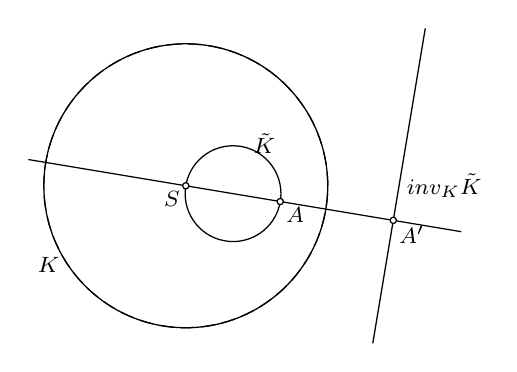
\begin{tikzpicture}
                % \clip (0,0) rectangle (14.000000,10.000000);
                {\footnotesize
                
                % Drawing circle k
                \draw [line width=0.016cm] (6.302776,3.500000) arc (0:2:1.802776 and 1.802776) -- (6.300638,3.587773);%
                \draw [line width=0.016cm] (6.300638,3.587773) -- (6.300305,3.594350) arc (3:5:1.802776 and 1.802776) -- (6.294229,3.675337);%
                \draw [line width=0.016cm] (6.283564,3.762486) -- (6.280580,3.782016) arc (9:11:1.802776 and 1.802776) -- (6.268669,3.849012);%
                \draw [line width=0.016cm] (6.268669,3.849012) -- (6.263381,3.874818) arc (12:13:1.802776 and 1.802776) -- (6.249579,3.934711);%
                \draw [line width=0.016cm] (6.226339,4.019378) -- (6.224003,4.027081) arc (17:19:1.802776 and 1.802776) -- (6.199004,4.102813);%
                \draw [line width=0.016cm] (6.199004,4.102813) -- (6.194055,4.116586) arc (20:22:1.802776 and 1.802776) -- (6.167640,4.184819);%
                \draw [line width=0.016cm] (6.132320,4.265200) -- (6.120324,4.290285) arc (26:27:1.802776 and 1.802776) -- (6.093128,4.343766);%
                \draw [line width=0.016cm] (6.093128,4.343766) -- (6.091756,4.346352) arc (28:30:1.802776 and 1.802776) -- (6.050158,4.420331);%
                \draw [line width=0.016cm] (6.003511,4.494713) -- (5.994569,4.508099) arc (34:36:1.802776 and 1.802776) -- (5.953298,4.566736);%
                \draw [line width=0.016cm] (5.953298,4.566736) -- (5.939761,4.584937) arc (37:39:1.802776 and 1.802776) -- (5.899637,4.636229);%
                \draw [line width=0.016cm] (5.842657,4.703026) -- (5.839723,4.706292) arc (42:44:1.802776 and 1.802776) -- (5.782492,4.766970);%
                \draw [line width=0.016cm] (5.782492,4.766970) -- (5.774755,4.774755) arc (45:47:1.802776 and 1.802776) -- (5.719286,4.827909);%
                \draw [line width=0.016cm] (5.653187,4.885698) -- (5.634524,4.901020) arc (51:53:1.802776 and 1.802776) -- (5.584353,4.940201);%
                \draw [line width=0.016cm] (5.584353,4.940201) -- (5.559645,4.958476) arc (54:55:1.802776 and 1.802776) -- (5.512947,4.991287);%
                \draw [line width=0.016cm] (5.439139,5.038837) -- (5.428498,5.045280) arc (59:61:1.802776 and 1.802776) -- (5.363103,5.082736);%
                \draw [line width=0.016cm] (5.363103,5.082736) -- (5.346352,5.091756) arc (62:64:1.802776 and 1.802776) -- (5.285019,5.122882);%
                \draw [line width=0.016cm] (5.205074,5.159178) -- (5.204401,5.159464) arc (67:69:1.802776 and 1.802776) -- (5.123457,5.191538);%
                \draw [line width=0.016cm] (5.123457,5.191538) -- (5.116586,5.194055) arc (70:72:1.802776 and 1.802776) -- (5.040360,5.219887);%
                \draw [line width=0.016cm] (4.955982,5.244156) -- (4.936131,5.249225) arc (76:78:1.802776 and 1.802776) -- (4.870523,5.264288);%
                \draw [line width=0.016cm] (4.870523,5.264288) -- (4.843986,5.269654) arc (79:80:1.802776 and 1.802776) -- (4.784184,5.280236);%
                \draw [line width=0.016cm] (4.697172,5.291961) -- (4.688441,5.292900) arc (84:86:1.802776 and 1.802776) -- (4.609692,5.299435);%
                \draw [line width=0.016cm] (4.609692,5.299435) -- (4.594350,5.300305) arc (87:89:1.802776 and 1.802776) -- (4.521951,5.302642);%
                \draw [line width=0.016cm] (4.434159,5.301573) -- (4.405650,5.300305) arc (93:94:1.802776 and 1.802776) -- (4.346523,5.296231);%
                \draw [line width=0.016cm] (4.346523,5.296231) -- (4.342878,5.295916) arc (95:97:1.802776 and 1.802776) -- (4.259251,5.286628);%
                \draw [line width=0.016cm] (4.172550,5.272788) -- (4.156014,5.269654) arc (101:103:1.802776 and 1.802776) -- (4.086625,5.254743);%
                \draw [line width=0.016cm] (4.086625,5.254743) -- (4.063869,5.249226) arc (104:106:1.802776 and 1.802776) -- (4.001681,5.232535);%
                \draw [line width=0.016cm] (3.917919,5.206219) -- (3.913074,5.204558) arc (109:111:1.802776 and 1.802776) -- (3.835538,5.175855);%
                \draw [line width=0.016cm] (3.835538,5.175855) -- (3.824669,5.171505) arc (112:114:1.802776 and 1.802776) -- (3.754732,5.141516);%
                \draw [line width=0.016cm] (3.675695,5.103284) -- (3.653648,5.091756) arc (118:120:1.802776 and 1.802776);%
                \draw [line width=0.016cm] (3.598612,5.061250) arc (120:122:1.802776 and 1.802776) -- (3.523668,5.015512);%
                \draw [line width=0.016cm] (3.451039,4.966179) -- (3.440355,4.958476) arc (126:128:1.802776 and 1.802776) -- (3.380898,4.913369);%
                \draw [line width=0.016cm] (3.380898,4.913369) -- (3.365477,4.901020) arc (129:131:1.802776 and 1.802776) -- (3.313412,4.857206);%
                \draw [line width=0.016cm] (3.248740,4.797825) -- (3.247687,4.796808) arc (134:136:1.802776 and 1.802776) -- (3.187036,4.735365);%
                \draw [line width=0.016cm] (3.187036,4.735365) -- (3.181534,4.729490) arc (137:139:1.802776 and 1.802776) -- (3.128446,4.669974);%
                \draw [line width=0.016cm] (3.073110,4.601809) -- (3.060239,4.584938) arc (143:145:1.802776 and 1.802776) -- (3.021157,4.531031);%
                \draw [line width=0.016cm] (3.021157,4.531031) -- (3.005431,4.508100) arc (146:147:1.802776 and 1.802776) -- (2.972713,4.457807);%
                \draw [line width=0.016cm] (2.927891,4.382311) -- (2.923257,4.374003) arc (151:153:1.802776 and 1.802776) -- (2.886798,4.304722);%
                \draw [line width=0.016cm] (2.886798,4.304722) -- (2.879676,4.290285) arc (154:156:1.802776 and 1.802776) -- (2.849531,4.225225);%
                \draw [line width=0.016cm] (2.816179,4.144007) -- (2.805945,4.116586) arc (160:161:1.802776 and 1.802776) -- (2.786820,4.061262);%
                \draw [line width=0.016cm] (2.786820,4.061262) -- (2.785459,4.057089) arc (162:164:1.802776 and 1.802776) -- (2.761526,3.977186);%
                \draw [line width=0.016cm] (2.740354,3.891978) -- (2.736619,3.874818) arc (168:170:1.802776 and 1.802776) -- (2.723357,3.805840);%
                \draw [line width=0.016cm] (2.723357,3.805840) -- (2.719420,3.782017) arc (171:173:1.802776 and 1.802776) -- (2.710573,3.718977);%
                \draw [line width=0.016cm] (2.702034,3.631594) -- (2.701616,3.625756) arc (176:178:1.802776 and 1.802776) -- (2.697759,3.543900);%
                \draw [line width=0.016cm] (2.697759,3.543900) -- (2.697499,3.531463) arc (179:181:1.802776 and 1.802776) -- (2.697759,3.456101);%
                \draw [line width=0.016cm] (2.702034,3.368407) -- (2.704084,3.342878) arc (185:186:1.802776 and 1.802776) -- (2.710573,3.281024);%
                \draw [line width=0.016cm] (2.710573,3.281024) -- (2.710662,3.280297) arc (187:189:1.802776 and 1.802776) -- (2.723356,3.194161);%
                \draw [line width=0.016cm] (2.740354,3.108023) -- (2.743429,3.094464) arc (193:195:1.802776 and 1.802776) -- (2.761525,3.022815);%
                \draw [line width=0.016cm] (2.761525,3.022815) -- (2.767061,3.003088) arc (196:198:1.802776 and 1.802776) -- (2.786820,2.938739);%
                \draw [line width=0.016cm] (2.816178,2.855994) -- (2.816964,2.853943) arc (201:203:1.802776 and 1.802776) -- (2.849530,2.774776);%
                \draw [line width=0.016cm] (2.849530,2.774776) -- (2.853082,2.766745) arc (204:206:1.802776 and 1.802776) -- (2.886797,2.695279);%
                \draw [line width=0.016cm] (2.927890,2.617690) -- (2.938750,2.598612) arc (210:212:1.802776 and 1.802776) -- (2.972712,2.542194);%
                \draw [line width=0.016cm] (2.972712,2.542194) -- (2.988065,2.518138) arc (213:214:1.802776 and 1.802776) -- (3.021157,2.468970);%
                \draw [line width=0.016cm] (3.073109,2.398192) -- (3.079393,2.390101) arc (218:220:1.802776 and 1.802776) -- (3.128445,2.330026);%
                \draw [line width=0.016cm] (3.128445,2.330026) -- (3.139428,2.317273) arc (221:223:1.802776 and 1.802776) -- (3.187035,2.264636);%
                \draw [line width=0.016cm] (3.248739,2.202176) -- (3.270510,2.181534) arc (227:228:1.802776 and 1.802776) -- (3.313411,2.142794);%
                \draw [line width=0.016cm] (3.313411,2.142794) -- (3.317272,2.139428) arc (229:231:1.802776 and 1.802776) -- (3.380897,2.086632);%
                \draw [line width=0.016cm] (3.451038,2.033822) -- (3.465970,2.023253) arc (235:237:1.802776 and 1.802776) -- (3.523667,1.984489);%
                \draw [line width=0.016cm] (3.523667,1.984489) -- (3.544674,1.971160) arc (238:239:1.802776 and 1.802776) -- (3.598611,1.938751);%
                \draw [line width=0.016cm] (3.675694,1.896716) -- (3.681557,1.893715) arc (243:245:1.802776 and 1.802776) -- (3.754731,1.858484);%
                \draw [line width=0.016cm] (3.754731,1.858484) -- (3.766745,1.853083) arc (246:248:1.802776 and 1.802776) -- (3.835537,1.824145);%
                \draw [line width=0.016cm] (3.917918,1.793782) -- (3.942911,1.785459) arc (252:253:1.802776 and 1.802776) -- (4.001680,1.767465);%
                \draw [line width=0.016cm] (4.001680,1.767465) -- (4.003087,1.767061) arc (254:256:1.802776 and 1.802776) -- (4.086624,1.745258);%
                \draw [line width=0.016cm] (4.172549,1.727212) -- (4.186951,1.724613) arc (260:262:1.802776 and 1.802776) -- (4.259250,1.713372);%
                \draw [line width=0.016cm] (4.259250,1.713372) -- (4.280297,1.710662) arc (263:265:1.802776 and 1.802776) -- (4.346522,1.703769);%
                \draw [line width=0.016cm] (4.434158,1.698427) -- (4.437084,1.698323) arc (268:270:1.802776 and 1.802776) -- (4.521950,1.697358);%
                \draw [line width=0.016cm] (4.521950,1.697358) -- (4.531462,1.697499) arc (271:273:1.802776 and 1.802776) -- (4.609691,1.700565);%
                \draw [line width=0.016cm] (4.697171,1.708039) -- (4.719703,1.710662) arc (277:279:1.802776 and 1.802776) -- (4.784183,1.719764);%
                \draw [line width=0.016cm] (4.784183,1.719764) -- (4.813048,1.724613) arc (280:281:1.802776 and 1.802776) -- (4.870522,1.735712);%
                \draw [line width=0.016cm] (4.955981,1.755844) -- (4.966592,1.758652) arc (285:287:1.802776 and 1.802776) -- (5.040359,1.780113);%
                \draw [line width=0.016cm] (5.040359,1.780113) -- (5.057088,1.785458) arc (288:290:1.802776 and 1.802776) -- (5.123456,1.808461);%
                \draw [line width=0.016cm] (5.205073,1.840822) -- (5.233254,1.853082) arc (294:295:1.802776 and 1.802776) -- (5.285018,1.877118);%
                \draw [line width=0.016cm] (5.285018,1.877118) -- (5.290284,1.879676) arc (296:298:1.802776 and 1.802776) -- (5.363102,1.917263);%
                \draw [line width=0.016cm] (5.439138,1.961163) -- (5.455325,1.971159) arc (302:304:1.802776 and 1.802776) -- (5.512946,2.008712);%
                \draw [line width=0.016cm] (5.512946,2.008712) -- (5.534029,2.023252) arc (305:306:1.802776 and 1.802776) -- (5.584352,2.059798);%
                \draw [line width=0.016cm] (5.653186,2.114301) -- (5.658801,2.118993) arc (310:312:1.802776 and 1.802776) -- (5.719285,2.172090);%
                \draw [line width=0.016cm] (5.719285,2.172090) -- (5.729490,2.181533) arc (313:315:1.802776 and 1.802776) -- (5.782492,2.233029);%
                \draw [line width=0.016cm] (5.842656,2.296973) -- (5.860572,2.317272) arc (319:320:1.802776 and 1.802776) -- (5.899637,2.363771);%
                \draw [line width=0.016cm] (5.899637,2.363771) -- (5.901019,2.365476) arc (321:323:1.802776 and 1.802776) -- (5.953297,2.433263);%
                \draw [line width=0.016cm] (6.003510,2.505286) -- (6.011935,2.518138) arc (327:329:1.802776 and 1.802776) -- (6.050158,2.579668);%
                \draw [line width=0.016cm] (6.050158,2.579668) -- (6.061249,2.598612) arc (330:332:1.802776 and 1.802776) -- (6.093128,2.656233);%
                \draw [line width=0.016cm] (6.132320,2.734799) -- (6.133869,2.738114) arc (335:337:1.802776 and 1.802776) -- (6.167640,2.815180);%
                \draw [line width=0.016cm] (6.167640,2.815180) -- (6.171504,2.824668) arc (338:340:1.802776 and 1.802776) -- (6.199004,2.897186);%
                \draw [line width=0.016cm] (6.226339,2.980621) -- (6.232939,3.003087) arc (344:346:1.802776 and 1.802776) -- (6.249579,3.065288);%
                \draw [line width=0.016cm] (6.249579,3.065288) -- (6.256570,3.094463) arc (347:348:1.802776 and 1.802776) -- (6.268669,3.150987);%
                \draw [line width=0.016cm] (6.283564,3.237513) -- (6.285231,3.249102) arc (352:354:1.802776 and 1.802776) -- (6.294229,3.324661);%
                \draw [line width=0.016cm] (6.294229,3.324661) -- (6.295915,3.342877) arc (355:357:1.802776 and 1.802776) -- (6.300638,3.412226);%
                \draw [line width=0.016cm] (6.302776,3.499999) -- (6.302776,3.499999) arc (360:360:1.802776 and 1.802776) --(6.302776,3.500000) arc (0:359:1.802776 and 1.802776) -- (6.302776,3.499999);%
                
                % Drawing line s
                \draw [line width=0.016cm] (2.500000,3.833333) -- (4.460544,3.506576);%
                \draw [line width=0.016cm] (4.539456,3.493424) -- (5.660544,3.306576);%
                \draw [line width=0.016cm] (5.739456,3.293424) -- (7.095679,3.067387);%
                \draw [line width=0.016cm] (7.174591,3.054235) -- (8.000000,2.916667);%
                
                % Drawing line u
                \draw [line width=0.016cm] (6.875000,1.500000) -- (7.128559,3.021355);%
                \draw [line width=0.016cm] (7.141711,3.100267) -- (7.541667,5.500000);%
                
                % Drawing circle o
                \draw [line width=0.016cm] (5.708276,3.400000) arc (0:166:0.608276 and 0.608276) -- (4.507870,3.539218);%
                \draw [line width=0.016cm] (4.494725,3.460349) -- (4.494038,3.453015) arc (175:346:0.608276 and 0.608276) -- (5.692130,3.260782);%
                \draw [line width=0.016cm] (5.705275,3.339650) -- (5.705962,3.346985) arc (355:359:0.608276 and 0.608276) -- (5.708276,3.400000);%
                
                % Marking point S by circle
                \draw [line width=0.016cm] (4.500000,3.500000) circle (0.040000);%
                \draw (4.530000,3.530000) node [anchor=north east] { $S$ };%
                
                % Marking point K
                \draw (3.000000,2.500000) node [anchor=east] { $K$ };%
                
                % Marking point A' by circle
                \draw [line width=0.016cm] (7.135135,3.060811) circle (0.040000);%
                \draw (7.105135,3.090811) node [anchor=north west] { $A'$ };%
                
                % Marking point A by circle
                \draw [line width=0.016cm] (5.700000,3.300000) circle (0.040000);%
                \draw (5.670000,3.330000) node [anchor=north west] { $A$ };%
                
                % Marking point \tilde{K}
                \draw (5.498669,3.800000) node [anchor=south] { $\tilde{K}$ };%
                
                % Marking point inv_K\tilde{K}
                \draw (7.200000,3.500000) node [anchor=west] { $inv_K\tilde{K}$ };%
                }
                \end{tikzpicture}
            \\ Velja: $inv_K\tilde{K}$ je premica pravokotna na $\overleftrightarrow{SA}$ v točki $A'$, kjer je $SA$ premer krožnice $\tilde{K}$ in $A'=inv_K A$.
        \item \uline{krožnica $\tilde{K}$ ne vsebuje $S$}:
            \begin{enumerate}
                \item \uline{$S$ leži izven $\tilde{K}$}:
                    \\ 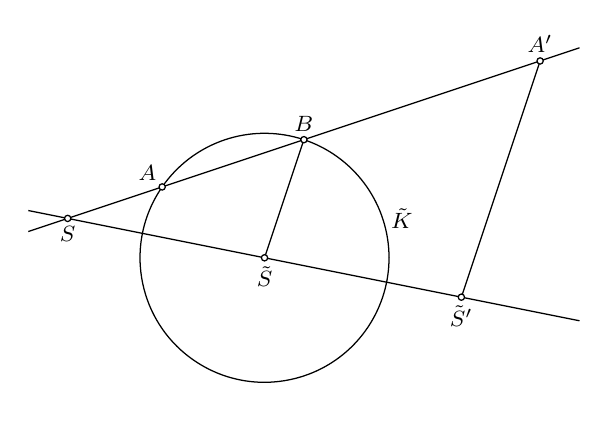
\begin{tikzpicture}
                        % \clip (0,0) rectangle (14.000000,10.000000);
                        {\footnotesize
                        
                        % Marking point S by circle
                        \draw [line width=0.016cm] (2.500000,3.500000) circle (0.040000);%
                        \draw (2.500000,3.500000) node [anchor=north] { $S$ };%
                        
                        % Marking point \tilde{S} by circle
                        \draw [line width=0.016cm] (5.000000,3.000000) circle (0.040000);%
                        \draw (5.000000,3.000000) node [anchor=north] { $\tilde{S}$ };%
                        
                        % Marking point \tilde{S}' by circle
                        \draw [line width=0.016cm] (7.500000,2.500000) circle (0.040000);%
                        \draw (7.500000,2.500000) node [anchor=north] { $\tilde{S}'$ };%
                        
                        % Marking point \tilde{K}
                        \draw (6.500000,3.500000) node [anchor=west] { $\tilde{K}$ };%
                        
                        % Marking point A by circle
                        \draw [line width=0.016cm] (3.700000,3.900000) circle (0.040000);%
                        \draw (3.730000,3.870000) node [anchor=south east] { $A$ };%
                        
                        % Marking point B by circle
                        \draw [line width=0.016cm] (5.500000,4.500000) circle (0.040000);%
                        \draw (5.500000,4.500000) node [anchor=south] { $B$ };%
                        
                        % Marking point A' by circle
                        \draw [line width=0.016cm] (8.500000,5.500000) circle (0.040000);%
                        \draw (8.500000,5.500000) node [anchor=south] { $A'$ };%
                        
                        % Drawing circle k'
                        \draw [line width=0.016cm] (6.581139,3.000000) arc (0:70:1.581139 and 1.581139) -- (5.537784,4.486872);%
                        \draw [line width=0.016cm] (5.461896,4.512168) -- (5.435821,4.519888) arc (74:143:1.581139 and 1.581139) -- (3.723183,3.932597);%
                        \draw [line width=0.016cm] (3.677649,3.866827) -- (3.673946,3.861150) arc (147:360:1.581139 and 1.581139) --(6.581139,3.000000) arc (0:0:1.581139 and 1.581139);%
                        
                        % Drawing line x
                        \draw [line width=0.016cm] (2.000000,3.333333) -- (2.462053,3.487351);%
                        \draw [line width=0.016cm] (2.537947,3.512649) -- (3.662053,3.887351);%
                        \draw [line width=0.016cm] (3.737947,3.912649) -- (5.462053,4.487351);%
                        \draw [line width=0.016cm] (5.537947,4.512649) -- (8.462053,5.487351);%
                        \draw [line width=0.016cm] (8.537947,5.512649) -- (9.000000,5.666667);%
                        
                        % Drawing line s
                        \draw [line width=0.016cm] (2.000000,3.600000) -- (2.460777,3.507845);%
                        \draw [line width=0.016cm] (2.539223,3.492155) -- (4.960777,3.007845);%
                        \draw [line width=0.016cm] (5.039223,2.992155) -- (7.460777,2.507845);%
                        \draw [line width=0.016cm] (7.539223,2.492155) -- (9.000000,2.200000);%
                        
                        % Drawing segment \tilde{S} B
                        \draw [line width=0.016cm] (5.012649,3.037947) -- (5.487351,4.462053);%
                        
                        % Drawing segment \tilde{S}' A'
                        \draw [line width=0.016cm] (7.512649,2.537947) -- (8.487351,5.462053);%
                        }
                        \end{tikzpicture}
                    \\ Velja: $|SA|\cdot |SA'|=r^2$. Naj bo $B$ drugo presečišče $\overrightarrow{SA}$ in $\tilde{K}$. Potem je $\frac{|SA'|}{|SB|}=\frac{r^2}{p}$ neodvisno od $A$. Naj bo $\tilde{S'}$ taka točka, da je: $S\ast \tilde{S}\ast \tilde{S'}$ in $\frac{|S\tilde{S'}|}{|S\tilde{S}|}=\frac{r^2}{p}$. Po kriteriju SKS dobimo podobnost: $\triangle A'S\tilde{S'}\sim\triangle BS\tilde{S}$ (skupen kot pri $S$). Sledi, da je $\frac{|A'\tilde{S'}|}{|B\tilde{S}|}=\frac{r^2}{p}$ oziroma $|A'\tilde{S'}|=\frac{r^2}{p}|B\tilde{S}|$ ($|B\tilde{S}|$ polmer $\tilde{K}$) neodvisno od $A$. Potem inverzi točk iz $\tilde{K}$ ležijo na krožnici s središčem v $\tilde{S'}$ in polmerom $\frac{r^2}{p}|B\tilde{S}|$. Ker je inverzija involucija, sledi, da je slika enaka tej krožnici.
                \item \uline{$S$ leži znotraj $\tilde{K}$:}
                    \\ 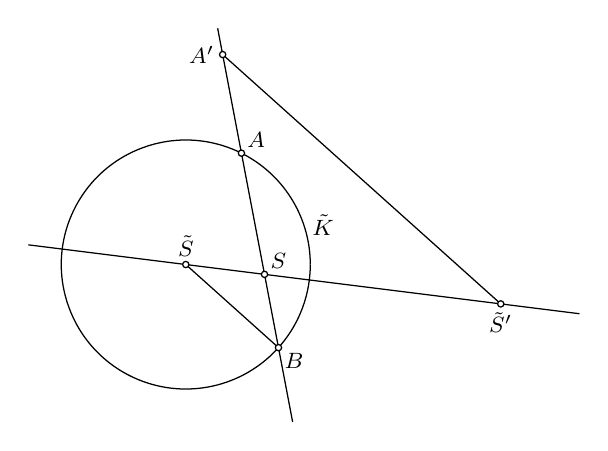
\begin{tikzpicture}
                        % \clip (0,0) rectangle (14.000000,10.000000);
                        {\footnotesize
                        
                        % Marking point S by circle
                        \draw [line width=0.016cm] (4.500000,3.375000) circle (0.040000);%
                        \draw (4.470000,3.345000) node [anchor=south west] { $S$ };%
                        
                        % Marking point \tilde{S} by circle
                        \draw [line width=0.016cm] (3.500000,3.500000) circle (0.040000);%
                        \draw (3.500000,3.500000) node [anchor=south] { $\tilde{S}$ };%
                        
                        % Marking point \tilde{S}' by circle
                        \draw [line width=0.016cm] (7.500000,3.000000) circle (0.040000);%
                        \draw (7.500000,3.000000) node [anchor=north] { $\tilde{S}'$ };%
                        
                        % Marking point \tilde{K}
                        \draw (5.000000,4.000000) node [anchor=west] { $\tilde{K}$ };%
                        
                        % Marking point A by circle
                        \draw [line width=0.016cm] (4.206786,4.914374) circle (0.040000);%
                        \draw (4.176786,4.884374) node [anchor=south west] { $A$ };%
                        
                        % Marking point B by circle
                        \draw [line width=0.016cm] (4.677240,2.444488) circle (0.040000);%
                        \draw (4.647240,2.474488) node [anchor=north west] { $B$ };%
                        
                        % Marking point A' by circle
                        \draw [line width=0.016cm] (3.968279,6.166535) circle (0.040000);%
                        \draw (3.968279,6.166535) node [anchor=east] { $A'$ };%
                        
                        % Drawing circle k'
                        \draw [line width=0.016cm] (5.081139,3.500000) arc (0:61:1.581139 and 1.581139) -- (4.242338,4.896042);%
                        \draw [line width=0.016cm] (4.170781,4.931800) -- (4.168218,4.932998) arc (65:316:1.581139 and 1.581139) -- (4.650163,2.415046);%
                        \draw [line width=0.016cm] (4.703564,2.474605) -- (4.711222,2.483663) arc (320:360:1.581139 and 1.581139);%
                        
                        % Drawing line x
                        \draw [line width=0.016cm] (4.857143,1.500000) -- (4.684725,2.405195);%
                        \draw [line width=0.016cm] (4.669756,2.483782) -- (4.507484,3.335706);%
                        \draw [line width=0.016cm] (4.492516,3.414294) -- (4.214270,4.875080);%
                        \draw [line width=0.016cm] (4.199301,4.953667) -- (3.975763,6.127242);%
                        \draw [line width=0.016cm] (3.960794,6.205829) -- (3.904762,6.500000);%
                        
                        % Drawing line s
                        \draw [line width=0.016cm] (1.500000,3.750000) -- (3.460309,3.504961);%
                        \draw [line width=0.016cm] (3.539691,3.495039) -- (4.460309,3.379961);%
                        \draw [line width=0.016cm] (4.539691,3.370039) -- (7.460309,3.004961);%
                        \draw [line width=0.016cm] (7.539691,2.995039) -- (8.500000,2.875000);%
                        
                        % Drawing segment \tilde{S} B
                        \draw [line width=0.016cm] (3.529782,3.473297) -- (4.647458,2.471191);%
                        
                        % Drawing segment \tilde{S}' A'
                        \draw [line width=0.016cm] (7.470218,3.026703) -- (3.998061,6.139833);%
                        }
                        \end{tikzpicture}
                    \\ Za poljuben $A\in\tilde{K}$ naj bo $A'$ inverz točke $A$ v $K$ in naj bo $B$ drugo presečišče $\overleftrightarrow{SA}$ s $\tilde{K}$. Potem velja $|SA|\cdot |SA'|=r^2$ in $|SA|\cdot |SB|=p, p<0,~potenca~S~na~\tilde{K}$ in od tod $\frac{|SA'|}{|SB|}=-\frac{r^2}{p}$. Izberimo $\tilde{S'}$ tako, da je $\tilde{S}\ast S\ast \tilde{S'}$ in $\frac{|S\tilde{S'}|}{|S\tilde{S}|}=-\frac{r^2}{p}$. Trikotnika $\triangle BS\tilde{S}\sim\triangle A'S\tilde{S'}$ sta podobna, ker imata sovršna kota pri $S$ in istoležni stranici v enakem razmerju: $\frac{|A'\tilde{S'}|}{|B\tilde{S}|}=-\frac{r^2}{p}$. Potem $\tilde{S}$ leži na krožnici s središčem v $\tilde{S'}$ in polmerom $-\frac{r^2}{p}|B\tilde{S}|$.
            \end{enumerate}
    \end{enumerate}

    \begin{izrek}
        Inverzija slika premice in krožnice v premice in krožnice. Slika je premica natanko tedaj, ko gre originalni objekt skozi središče inverzije.
    \end{izrek}

    \begin{trditev}
        Inverzija preslika poljuben kot na nasportno usmerjen skladen kot.
    \end{trditev}

        \begin{dokaz}
            \\ Naj bo $K$ krožnica inverzije s središčem $S$ in polmerom $r$, $A\neq S$ in naj bo dan kot $\angle BAC$.
            \\(1) $A \notin K$
            \\ 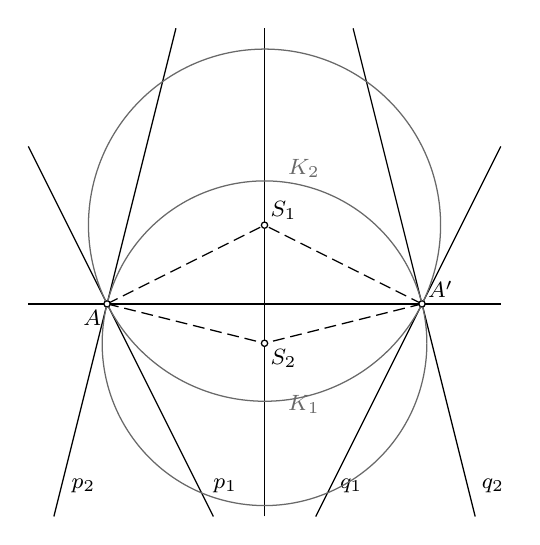
\begin{tikzpicture}
                % \clip (0,0) rectangle (14.000000,10.000000);
                {\footnotesize
                
                % Drawing line a
                \draw [line width=0.016cm] (1.000000,4.000000) -- (1.960000,4.000000);%
                \draw [line width=0.016cm] (2.040000,4.000000) -- (5.960000,4.000000);%
                \draw [line width=0.016cm] (6.040000,4.000000) -- (7.000000,4.000000);%
                
                % Drawing line s
                \draw [line width=0.016cm] (4.000000,1.300000) -- (4.000000,3.460000);%
                \draw [line width=0.016cm] (4.000000,3.540000) -- (4.000000,4.960000);%
                \draw [line width=0.016cm] (4.000000,5.040000) -- (4.000000,7.500000);%
                
                % Drawing line P1
                \draw [line width=0.016cm] (3.350000,1.300000) -- (2.017889,3.964223);%
                \draw [line width=0.016cm] (1.982111,4.035777) -- (1.000000,6.000000);%
                
                % Drawing line P2
                \draw [line width=0.016cm] (1.325000,1.300000) -- (1.990299,3.961194);%
                \draw [line width=0.016cm] (2.009701,4.038806) -- (2.875000,7.500000);%
                
                % Drawing line Q1
                \draw [line width=0.016cm] (4.650000,1.300000) -- (5.982111,3.964223);%
                \draw [line width=0.016cm] (6.017889,4.035777) -- (7.000000,6.000000);%
                
                % Drawing line Q2
                \draw [line width=0.016cm] (6.675000,1.300000) -- (6.009701,3.961194);%
                \draw [line width=0.016cm] (5.990299,4.038806) -- (5.125000,7.500000);%
                
                % Marking point A by circle
                \draw [line width=0.016cm] (2.000000,4.000000) circle (0.040000);%
                \draw (2.030000,4.030000) node [anchor=north east] { $A$ };%
                
                % Marking point A' by circle
                \draw [line width=0.016cm] (6.000000,4.000000) circle (0.040000);%
                \draw (5.970000,3.970000) node [anchor=south west] { $A'$ };%
                
                % Marking point S_1 by circle
                \draw [line width=0.016cm] (4.000000,5.000000) circle (0.040000);%
                \draw (3.970000,4.970000) node [anchor=south west] { $S_1$ };%
                
                % Marking point S_2 by circle
                \draw [line width=0.016cm] (4.000000,3.500000) circle (0.040000);%
                \draw (3.970000,3.530000) node [anchor=north west] { $S_2$ };%
                
                % Drawing segment A S_1
                \draw [line width=0.016cm] (2.035777,4.017889) -- (2.134164,4.067082);%
                \draw [line width=0.016cm] (2.201246,4.100623) -- (2.335410,4.167705);%
                \draw [line width=0.016cm] (2.402492,4.201246) -- (2.536656,4.268328);%
                \draw [line width=0.016cm] (2.603738,4.301869) -- (2.737902,4.368951);%
                \draw [line width=0.016cm] (2.804984,4.402492) -- (2.939149,4.469574);%
                \draw [line width=0.016cm] (3.006231,4.503115) -- (3.140395,4.570197);%
                \draw [line width=0.016cm] (3.207477,4.603738) -- (3.341641,4.670820);%
                \draw [line width=0.016cm] (3.408723,4.704361) -- (3.542887,4.771443);%
                \draw [line width=0.016cm] (3.609969,4.804984) -- (3.744133,4.872067);%
                \draw [line width=0.016cm] (3.811215,4.905608) -- (3.945379,4.972690);%
                
                % Drawing segment A' S_1
                \draw [line width=0.016cm] (5.964223,4.017889) -- (5.865836,4.067082);%
                \draw [line width=0.016cm] (5.798754,4.100623) -- (5.664590,4.167705);%
                \draw [line width=0.016cm] (5.597508,4.201246) -- (5.463344,4.268328);%
                \draw [line width=0.016cm] (5.396262,4.301869) -- (5.262098,4.368951);%
                \draw [line width=0.016cm] (5.195016,4.402492) -- (5.060851,4.469574);%
                \draw [line width=0.016cm] (4.993769,4.503115) -- (4.859605,4.570197);%
                \draw [line width=0.016cm] (4.792523,4.603738) -- (4.658359,4.670820);%
                \draw [line width=0.016cm] (4.591277,4.704361) -- (4.457113,4.771443);%
                \draw [line width=0.016cm] (4.390031,4.804984) -- (4.255867,4.872067);%
                \draw [line width=0.016cm] (4.188785,4.905608) -- (4.054621,4.972690);%
                
                % Drawing segment A S_2
                \draw [line width=0.016cm] (2.038806,3.990299) -- (2.145521,3.963620);%
                \draw [line width=0.016cm] (2.218282,3.945429) -- (2.363803,3.909049);%
                \draw [line width=0.016cm] (2.436564,3.890859) -- (2.582086,3.854479);%
                \draw [line width=0.016cm] (2.654846,3.836288) -- (2.800368,3.799908);%
                \draw [line width=0.016cm] (2.873128,3.781718) -- (3.018650,3.745338);%
                \draw [line width=0.016cm] (3.091410,3.727147) -- (3.236932,3.690767);%
                \draw [line width=0.016cm] (3.309692,3.672577) -- (3.455214,3.636197);%
                \draw [line width=0.016cm] (3.527974,3.618006) -- (3.673496,3.581626);%
                \draw [line width=0.016cm] (3.746257,3.563436) -- (3.891778,3.527056);%
                
                % Drawing segment A' S_2
                \draw [line width=0.016cm] (5.961194,3.990299) -- (5.854479,3.963620);%
                \draw [line width=0.016cm] (5.781718,3.945429) -- (5.636197,3.909049);%
                \draw [line width=0.016cm] (5.563436,3.890859) -- (5.417914,3.854479);%
                \draw [line width=0.016cm] (5.345154,3.836288) -- (5.199632,3.799908);%
                \draw [line width=0.016cm] (5.126872,3.781718) -- (4.981350,3.745338);%
                \draw [line width=0.016cm] (4.908590,3.727147) -- (4.763068,3.690767);%
                \draw [line width=0.016cm] (4.690308,3.672577) -- (4.544786,3.636197);%
                \draw [line width=0.016cm] (4.472026,3.618006) -- (4.326504,3.581626);%
                \draw [line width=0.016cm] (4.253743,3.563436) -- (4.108222,3.527056);%
                
                % Marking point p_1
                \draw (3.500000,1.500000) node [anchor=south] { $p_1$ };%
                
                % Marking point p_2
                \draw (1.700000,1.500000) node [anchor=south] { $p_2$ };%
                
                % Marking point q_1
                \draw (5.100000,1.500000) node [anchor=south] { $q_1$ };%
                
                % Marking point q_2
                \draw (6.900000,1.500000) node [anchor=south] { $q_2$ };%
                
                % Changing color 105 105 105
                \definecolor{r105g105b105}{rgb}{0.411765,0.411765,0.411765}%
                \color{r105g105b105}% 
                
                % Drawing circle k1
                \draw [line width=0.016cm] (6.236068,5.000000) arc (0:205:2.236068 and 2.236068) -- (1.982432,4.035936);%
                \draw [line width=0.016cm] (2.018208,3.964385) -- (2.025669,3.950230) arc (208:332:2.236068 and 2.236068) -- (5.981792,3.964384);%
                \draw [line width=0.016cm] (6.017568,4.035935) -- (6.026566,4.054996) arc (335:359:2.236068 and 2.236068) -- (6.236068,4.999999);%
                
                % Drawing circle k2
                \draw [line width=0.016cm] (6.061553,3.500000) arc (0:12:2.061553 and 2.061553) -- (6.009324,3.961102);%
                \draw [line width=0.016cm] (5.989923,4.038710) -- (5.981692,4.068241) arc (16:164:2.061553 and 2.061553) -- (2.010077,4.038710);%
                \draw [line width=0.016cm] (1.990676,3.961102) -- (1.983497,3.928621) arc (168:360:2.061553 and 2.061553);%
                
                % Marking point K_2
                \draw (4.500000,5.500000) node [anchor=south] { $K_2$ };%
                
                % Marking point K_1
                \draw (4.500000,2.500000) node [anchor=south] { $K_1$ };%
                \color{black}
                }
                \end{tikzpicture}
            \\ Naj bo $A'$ inverz $A$ v $K$. Za $i=1,2$ naj bo $K_i$ krožnica skozi $A$ in $A'$, ki je v $A$ tangentna na premico $p_i$. $K_i$ je enolično določena, saj je njeno središče $S_i$ presek simetrale daljice $AA'$ in pravokotnice na $p_i$ v $A$. Ker je $A,A'\in K_i$, iz trditve o pravokotnih krožnicah sledi, da inverzija v $K$ preslika $K_i$ nazaj vase. Posledično kot med $p_1$ in $p_2$, ki je kot med $K_1$ in $K_2$ v $A$, preslika v kot med $K_1$ in $K_2$ v $A'$, oziroma kot med njunima tangentama $q_1$ in $q_2$ v $A'$. Posledično zrcaljenje v simetrali daljice $AA'$ preslika tangenti $p_i$ v tangenti $q_i$ in s tem začetni kot v skladen, nasprotno usmerjen kot.
            \\ (2) $A\in K$
            \\ 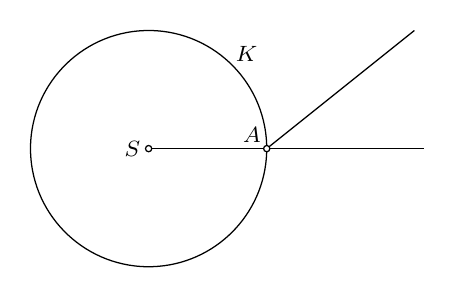
\begin{tikzpicture}
                % \clip (0,0) rectangle (14.000000,10.000000);
                {\footnotesize
                
                % Drawing circle S A
                \draw [line width=0.016cm] (4.499467,3.039996) -- (4.499086,3.052349) arc (2:358:1.500000 and 1.500000) -- (4.499467,2.960003);%
                
                % Drawing segment S Y
                \draw [line width=0.016cm] (3.040000,3.000000) -- (4.460000,3.000000);%
                \draw [line width=0.016cm] (4.540000,3.000000) -- (6.500000,3.000000);%
                
                % Drawing segment A X
                \draw [line width=0.016cm] (4.531235,3.024988) -- (6.375000,4.500000);%
                
                % Marking point S by circle
                \draw [line width=0.016cm] (3.000000,3.000000) circle (0.040000);%
                \draw (3.000000,3.000000) node [anchor=east] { $S$ };%
                
                % Marking point A by circle
                \draw [line width=0.016cm] (4.500000,3.000000) circle (0.040000);%
                \draw (4.530000,2.970000) node [anchor=south east] { $A$ };%
                
                % Marking point K
                \draw (4.000000,4.000000) node [anchor=south west] { $K$ };%
                }
                \end{tikzpicture}
            \\ V tem primeru merimo kot od poltraka $\overrightarrow{SA}$.
            \\ (2a):
            \\ 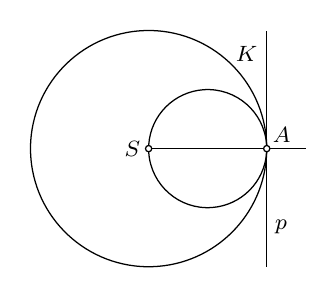
\begin{tikzpicture}
                % \clip (0,0) rectangle (14.000000,10.000000);
                {\footnotesize
                
                % Drawing circle S A
                \draw [line width=0.016cm] (4.499467,3.039996) -- (4.499086,3.052349) arc (2:358:1.500000 and 1.500000) -- (4.499467,2.960003);%
                
                % Drawing circle U A
                \draw [line width=0.016cm] (4.498933,3.039986) -- (4.498173,3.052317) arc (4:176:0.750000 and 0.750000) -- (3.001067,3.039986);%
                \draw [line width=0.016cm] (3.001067,2.960014) -- (3.001827,2.947683) arc (184:356:0.750000 and 0.750000) -- (4.498933,2.960014);%
                
                % Drawing segment S Y
                \draw [line width=0.016cm] (3.040000,3.000000) -- (4.460000,3.000000);%
                \draw [line width=0.016cm] (4.540000,3.000000) -- (5.000000,3.000000);%
                
                % Drawing line u
                \draw [line width=0.016cm] (4.500000,1.500000) -- (4.500000,2.960000);%
                \draw [line width=0.016cm] (4.500000,3.040000) -- (4.500000,4.500000);%
                
                % Marking point S by circle
                \draw [line width=0.016cm] (3.000000,3.000000) circle (0.040000);%
                \draw (3.000000,3.000000) node [anchor=east] { $S$ };%
                
                % Marking point A by circle
                \draw [line width=0.016cm] (4.500000,3.000000) circle (0.040000);%
                \draw (4.470000,2.970000) node [anchor=south west] { $A$ };%
                
                % Marking point K
                \draw (4.000000,4.000000) node [anchor=south west] { $K$ };%
                
                % Marking point p
                \draw (4.500000,2.000000) node [anchor=west] { $p$ };%
                }
                \end{tikzpicture}
            \\ Pri $A$ je pravi kot, določen s premico $p$. Inverz $p$ v $K$ je krožnica s premerom $SA$. Inverzija ta kot spet preslika v pravi kot (tangenta na inverzno krožnico v $A$ je $p$), ki je nasprotno usmerjen.
            \\ (2b): 
            \\ 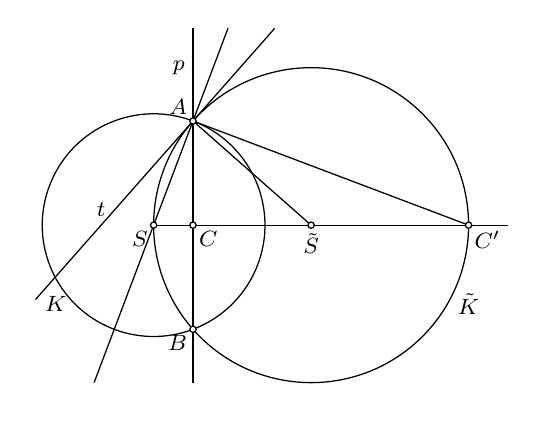
\begin{tikzpicture}
                % \clip (0,0) rectangle (14.000000,10.000000);
                {\footnotesize
                
                % Drawing circle k
                \draw [line width=0.016cm] (3.914214,3.500000) arc (0:67:1.414214 and 1.414214) -- (3.037213,4.808206);%
                \draw [line width=0.016cm] (2.962387,4.836487) -- (2.960423,4.837165) arc (71:289:1.414214 and 1.414214) -- (2.962387,2.163513);%
                \draw [line width=0.016cm] (3.037212,2.191794) -- (3.052577,2.198209) arc (293:360:1.414214 and 1.414214) --(3.914214,3.500000) arc (0:0:1.414214 and 1.414214);%
                
                % Drawing segment S L
                \draw [line width=0.016cm] (2.540000,3.500000) -- (2.960000,3.500000);%
                \draw [line width=0.016cm] (3.040000,3.500000) -- (4.460000,3.500000);%
                \draw [line width=0.016cm] (4.540000,3.500000) -- (6.460000,3.500000);%
                \draw [line width=0.016cm] (6.540000,3.500000) -- (7.000000,3.500000);%
                
                % Drawing segment A C'
                \draw [line width=0.016cm] (3.037417,4.808734) -- (6.462583,3.514142);%
                
                % Drawing line t
                \draw [line width=0.016cm] (3.000000,1.500000) -- (3.000000,2.137124);%
                \draw [line width=0.016cm] (3.000000,2.217124) -- (3.000000,3.460000);%
                \draw [line width=0.016cm] (3.000000,3.540000) -- (3.000000,4.782876);%
                \draw [line width=0.016cm] (3.000000,4.862876) -- (3.000000,6.000000);%
                
                % Drawing circle k'
                \draw [line width=0.016cm] (6.499600,3.539998) -- (6.498782,3.569799) arc (2:137:2.000000 and 2.000000) -- (3.026756,4.852610);%
                \draw [line width=0.016cm] (2.973844,4.792613) -- (2.967911,4.785575) arc (140:178:2.000000 and 2.000000) -- (2.500400,3.539998);%
                \draw [line width=0.016cm] (2.500400,3.460003) -- (2.501218,3.430201) arc (182:220:2.000000 and 2.000000) -- (2.973843,2.207388);%
                \draw [line width=0.016cm] (3.026756,2.147391) -- (3.037292,2.136004) arc (223:358:2.000000 and 2.000000) -- (6.499600,3.460001);%
                
                % Drawing segment \tilde{S} A
                \draw [line width=0.016cm] (4.470000,3.526458) -- (3.030000,4.796418);%
                
                % Drawing line n
                \draw [line width=0.016cm] (4.038126,6.000000) -- (3.026458,4.852876);%
                \draw [line width=0.016cm] (2.973542,4.792876) -- (1.000000,2.555089);%
                
                % Drawing line R
                \draw [line width=0.016cm] (1.744071,1.500000) -- (2.485858,3.462583);%
                \draw [line width=0.016cm] (2.514142,3.537417) -- (2.985858,4.785459);%
                \draw [line width=0.016cm] (3.014142,4.860292) -- (3.444911,6.000000);%
                
                % Marking point p
                \draw (3.000000,5.500000) node [anchor=east] { $p$ };%
                
                % Marking point t
                \draw (1.833333,3.500000) node [anchor=south] { $t$ };%
                
                % Marking point S by circle
                \draw [line width=0.016cm] (2.500000,3.500000) circle (0.040000);%
                \draw (2.530000,3.530000) node [anchor=north east] { $S$ };%
                
                % Marking point K
                \draw (1.500000,2.500000) node [anchor=east] { $K$ };%
                
                % Marking point A by circle
                \draw [line width=0.016cm] (3.000000,4.822876) circle (0.040000);%
                \draw (3.030000,4.792876) node [anchor=south east] { $A$ };%
                
                % Marking point B by circle
                \draw [line width=0.016cm] (3.000000,2.177124) circle (0.040000);%
                \draw (3.030000,2.207124) node [anchor=north east] { $B$ };%
                
                % Marking point C' by circle
                \draw [line width=0.016cm] (6.500000,3.500000) circle (0.040000);%
                \draw (6.470000,3.530000) node [anchor=north west] { $C'$ };%
                
                % Marking point C by circle
                \draw [line width=0.016cm] (3.000000,3.500000) circle (0.040000);%
                \draw (2.970000,3.530000) node [anchor=north west] { $C$ };%
                
                % Marking point \tilde{K}
                \draw (6.500000,2.500000) node  { $\tilde{K}$ };%
                
                % Marking point \tilde{S} by circle
                \draw [line width=0.016cm] (4.500000,3.500000) circle (0.040000);%
                \draw (4.500000,3.500000) node [anchor=north] { $\tilde{S}$ };%
                }
                \end{tikzpicture}
            \\ Kot pri $A$ ni pravi kot. Naj bo $\tilde{K}$ inverz premice $p$ v $K$ in $\tilde{S}$ njeno središče. Ker sta $C$ in $C'$ inverzni glede na $K$, sta trikotnika $\triangle SCA$ in $\triangle SAC'$ podobna, potem je $|\angle SC'A|=|\angle SAC|$. Naj bo $t$ tangenta na $\tilde{K}$ v $A$. Potem je $t\perp \overleftrightarrow{\tilde{S}A}$. Ker je kot $\angle SAC'$ pravi kot, je tudi njemu suplementaren kot pravi. Zato iz $|\angle \tilde{S}AC'|=|\angle SAC|$ sledi, da je kot med $\overrightarrow{SA}$ in $t$ tudi enak $|\angle SAC|$.
        \end{dokaz}

    \begin{opomba}
        Inverzija ohranja kote, zato je konformna preslikava.
    \end{opomba}

    V koordinatni obravnavi sledi, da je inverzija tesno povezana z Möbiusovimi transformacijami ravnine.

    Splošna Möbiusova transformacija je oblike $f(z)=\frac{az+b}{cz+d}$ in je sestavljena iz translacij $z\mapsto z+k; k\in \CC$, raztegov $z \mapsto m\cdot z; m\in\CC$ in $z\mapsto \frac{1}{z}$.
    
    Zapis inverzije s pomočjo kompleksnih števil: 
    $z'$ inverz  $z$, zato je pozitiven večkratnik $z$ $\to$ $z'=k\cdot z; k>0$. Ker je $z'$ inverz, vemo, da je $|z'|\cdot |z|=r^2$ in od tod $|z'|=\frac{r^2}{|z|}$. Potem velja: $|z'|=|kz|=k\cdot |z| \rightarrow k=\frac{|z'|}{|z|}=\frac{r^2}{|z|^2}=\frac{r^2}{z\cdot \overline{z}}$. Sledi, da je $z'=\frac{r^2}{\overline{z}}$.

\section{Nekateri pomembni rezultati evklidske geometrije}

    \subsection*{Težiščnice in težišče}

        \begin{definicija}
            Naj bo dan trikotnik $\triangle ABC$. Označimo razpolovišča stranic nasproti oglišč $A$, $B$ in $C$ z $A'$, $B'$ in $C'$. \textbf{Težiščnica} je daljica od oglišča do razpolovišča oglišču nasprotne stranice.
        \end{definicija}

            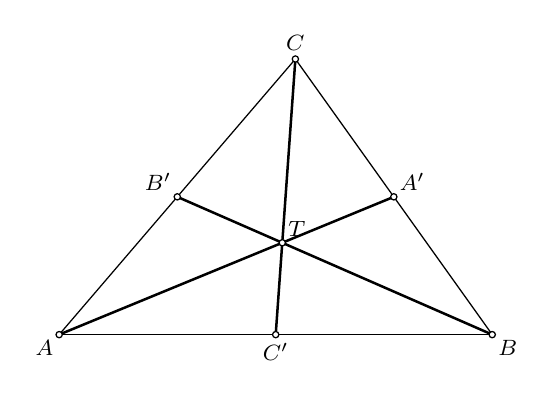
\begin{tikzpicture}
                % \clip (0,0) rectangle (14.000000,10.000000);
                {\footnotesize
                
                % Drawing segment A B
                \draw [line width=0.016cm] (1.540000,1.500000) -- (4.210000,1.500000);%
                \draw [line width=0.016cm] (4.290000,1.500000) -- (6.960000,1.500000);%
                
                % Drawing segment A C
                \draw [line width=0.016cm] (1.526032,1.530370) -- (2.973968,3.219630);%
                \draw [line width=0.016cm] (3.026032,3.280370) -- (4.473968,4.969630);%
                
                % Drawing segment B C
                \draw [line width=0.016cm] (6.976750,1.532549) -- (5.773250,3.217451);%
                \draw [line width=0.016cm] (5.726750,3.282549) -- (4.523250,4.967451);%
                
                % Marking point A by circle
                \draw [line width=0.016cm] (1.500000,1.500000) circle (0.040000);%
                \draw (1.530000,1.530000) node [anchor=north east] { $A$ };%
                
                % Marking point B by circle
                \draw [line width=0.016cm] (7.000000,1.500000) circle (0.040000);%
                \draw (6.970000,1.530000) node [anchor=north west] { $B$ };%
                
                % Marking point C by circle
                \draw [line width=0.016cm] (4.500000,5.000000) circle (0.040000);%
                \draw (4.500000,5.000000) node [anchor=south] { $C$ };%
                
                % Marking point A' by circle
                \draw [line width=0.016cm] (5.750000,3.250000) circle (0.040000);%
                \draw (5.720000,3.220000) node [anchor=south west] { $A'$ };%
                
                % Marking point B' by circle
                \draw [line width=0.016cm] (3.000000,3.250000) circle (0.040000);%
                \draw (3.030000,3.220000) node [anchor=south east] { $B'$ };%
                
                % Marking point C' by circle
                \draw [line width=0.016cm] (4.250000,1.500000) circle (0.040000);%
                \draw (4.250000,1.500000) node [anchor=north] { $C'$ };%
                
                % Marking point T by circle
                \draw [line width=0.016cm] (4.333333,2.666667) circle (0.040000);%
                \draw (4.303333,2.636667) node [anchor=south west] { $T$ };%
                
                % Drawing segment A A'
                \draw [line width=0.032cm] (1.536987,1.515230) -- (4.296346,2.651437);%
                \draw [line width=0.032cm] (4.370320,2.681897) -- (5.713013,3.234770);%
                
                % Drawing segment B B'
                \draw [line width=0.032cm] (6.963354,1.516033) -- (4.369980,2.650634);%
                \draw [line width=0.032cm] (4.296687,2.682699) -- (3.036646,3.233967);%
                
                % Drawing segment C C'
                \draw [line width=0.032cm] (4.497150,4.960102) -- (4.336183,2.706565);%
                \draw [line width=0.032cm] (4.330483,2.626768) -- (4.252850,1.539898);%
                }
            \end{tikzpicture}
            
        \begin{izrek}
            Težiščnice se sekajo v eni točki $T$ in ta točka $T$ deli vsako izmed težiščnic v razmerju $2:1$: $\frac{|AT|}{|A'T|}=\frac{|BT|}{|B'T|}=\frac{|CT|}{|C'T|}=\frac{2}{1}$.
        \end{izrek}

            \begin{dokaz}
                \\
                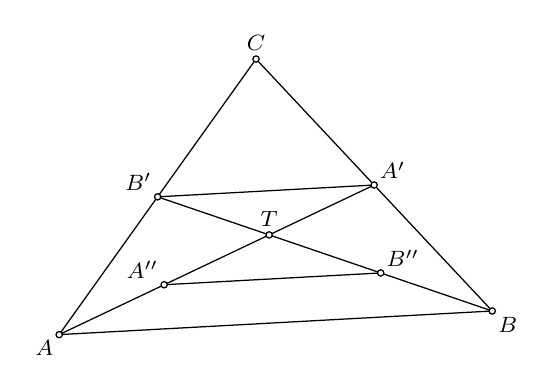
\begin{tikzpicture}
                    % \clip (0,0) rectangle (14.000000,10.000000);
                    {\footnotesize
                    
                    % Drawing segment A B
                    \draw [line width=0.016cm] (1.539941,1.502179) -- (6.960059,1.797821);%
                    
                    % Drawing segment A C
                    \draw [line width=0.016cm] (1.523250,1.532549) -- (2.726750,3.217451);%
                    \draw [line width=0.016cm] (2.773250,3.282549) -- (3.976750,4.967451);%
                    
                    % Drawing segment B C
                    \draw [line width=0.016cm] (6.972642,1.829181) -- (5.527358,3.370819);%
                    \draw [line width=0.016cm] (5.472642,3.429181) -- (4.027358,4.970819);%
                    
                    % Drawing segment A A'
                    \draw [line width=0.016cm] (1.536131,1.517162) -- (2.797202,2.116171);%
                    \draw [line width=0.016cm] (2.869464,2.150496) -- (4.130536,2.749504);%
                    \draw [line width=0.016cm] (4.202798,2.783829) -- (5.463869,3.382838);%
                    
                    % Drawing segment B B'
                    \draw [line width=0.016cm] (6.962143,1.812916) -- (5.621191,2.270417);%
                    \draw [line width=0.016cm] (5.545476,2.296249) -- (4.204524,2.753751);%
                    \draw [line width=0.016cm] (4.128809,2.779583) -- (2.787857,3.237084);%
                    
                    % Drawing segment A' B'
                    \draw [line width=0.016cm] (5.460059,3.397821) -- (2.789941,3.252179);%
                    
                    % Drawing segment A'' B''
                    \draw [line width=0.016cm] (2.873274,2.135512) -- (5.543393,2.281155);%
                    
                    % Marking point A by circle
                    \draw [line width=0.016cm] (1.500000,1.500000) circle (0.040000);%
                    \draw (1.530000,1.530000) node [anchor=north east] { $A$ };%
                    
                    % Marking point B by circle
                    \draw [line width=0.016cm] (7.000000,1.800000) circle (0.040000);%
                    \draw (6.970000,1.830000) node [anchor=north west] { $B$ };%
                    
                    % Marking point C by circle
                    \draw [line width=0.016cm] (4.000000,5.000000) circle (0.040000);%
                    \draw (4.000000,5.000000) node [anchor=south] { $C$ };%
                    
                    % Marking point A' by circle
                    \draw [line width=0.016cm] (5.500000,3.400000) circle (0.040000);%
                    \draw (5.470000,3.370000) node [anchor=south west] { $A'$ };%
                    
                    % Marking point B' by circle
                    \draw [line width=0.016cm] (2.750000,3.250000) circle (0.040000);%
                    \draw (2.780000,3.220000) node [anchor=south east] { $B'$ };%
                    
                    % Marking point T by circle
                    \draw [line width=0.016cm] (4.166667,2.766667) circle (0.040000);%
                    \draw (4.166667,2.766667) node [anchor=south] { $T$ };%
                    
                    % Marking point A'' by circle
                    \draw [line width=0.016cm] (2.833333,2.133333) circle (0.040000);%
                    \draw (2.863333,2.103333) node [anchor=south east] { $A''$ };%
                    
                    % Marking point B'' by circle
                    \draw [line width=0.016cm] (5.583333,2.283333) circle (0.040000);%
                    \draw (5.553333,2.253333) node [anchor=south west] { $B''$ };%
                    }
                \end{tikzpicture}
                \\ Označimo presečišče daljic $AA'$ in $BB'$ s $T$. Po kriteriju SKS za podobnost sta trikotnika $\triangle ACB$ in $\triangle B'CA'$ podobna: skupen kot pri $C$ in $\frac{|B'C|}{|AC|}=\frac{1}{2}=\frac{|CA'|}{|CB|}$. Ker velja $\angle CB'A'\cong\angle CAB$, sledi: $\overleftrightarrow{B'A'}\parallel\overleftrightarrow{AB}$. Naj bo $A''$ razpolovišče $AT$ in $B''$ razpolovišče $BT$. Potem sta trikotnika $\triangle ABT$ in $\triangle A''B''T$ podobna (s faktorjem $0.5$) in zato je $\overleftrightarrow{A''B''}\parallel\overleftrightarrow{AB}$. Sledi: $|A'B'|=\frac{1}{2}|AB|=|A''B''|$, torej je $|A'B'|\cong|A''B''|$. Poleg tega so v trikotnikih $\triangle A'B'T$ in $\triangle A''B''T$ istoležni koti skladni in od tod sledi skladnost trikotnikov $\triangle A'B'T\cong\triangle A''B''T$. Iz tega: $A'T\cong A''T\cong AA''$. Iz celotnega sledi $\frac{|A'T|}{|AT|}=\frac{1}{2}$. Ker enak sklep velja za poljuben par težiščnic, sledi, da je točka $T$ enolično določena kot točka, ki deli težiščnice v razmerju $2:1$ in leži na vseh treh.
            \end{dokaz}

            Alternativni dokaz obstoja težišča s pomočjo ploščin:

            \begin{dokaz}
                \\
                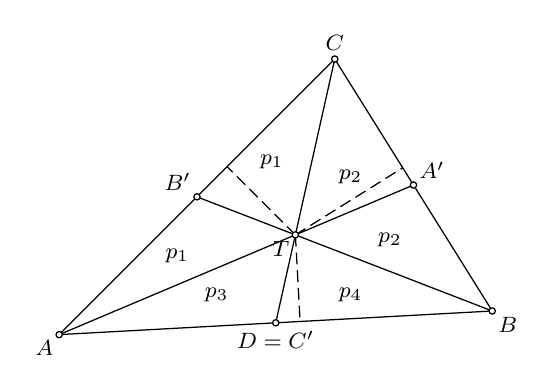
\begin{tikzpicture}
                    % \clip (0,0) rectangle (14.000000,10.000000);
                    {\footnotesize
                    
                    % Drawing segment A B
                    \draw [line width=0.016cm] (1.539941,1.502179) -- (4.210059,1.647821);%
                    \draw [line width=0.016cm] (4.289941,1.652179) -- (6.960059,1.797821);%
                    
                    % Drawing segment A C
                    \draw [line width=0.016cm] (1.528284,1.528284) -- (3.221716,3.221716);%
                    \draw [line width=0.016cm] (3.278284,3.278284) -- (4.971716,4.971716);%
                    
                    % Drawing segment B C
                    \draw [line width=0.016cm] (6.978800,1.833920) -- (6.021200,3.366080);%
                    \draw [line width=0.016cm] (5.978800,3.433920) -- (5.021200,4.966080);%
                    
                    % Drawing segment A A'
                    \draw [line width=0.016cm] (1.536850,1.515559) -- (4.463150,2.751108);%
                    \draw [line width=0.016cm] (4.536850,2.782226) -- (5.963150,3.384441);%
                    
                    % Drawing segment B B'
                    \draw [line width=0.016cm] (6.962692,1.814426) -- (4.537308,2.752241);%
                    \draw [line width=0.016cm] (4.462692,2.781092) -- (3.287308,3.235574);%
                    
                    % Drawing segment C C'
                    \draw [line width=0.016cm] (4.991261,4.960966) -- (4.508739,2.805700);%
                    \draw [line width=0.016cm] (4.491261,2.727633) -- (4.258739,1.689034);%
                    
                    % Drawing segment T N
                    \draw [line width=0.016cm] (4.471716,2.794951) -- (4.393934,2.872733);%
                    \draw [line width=0.016cm] (4.340901,2.925766) -- (4.234835,3.031832);%
                    \draw [line width=0.016cm] (4.181802,3.084865) -- (4.075736,3.190931);%
                    \draw [line width=0.016cm] (4.022703,3.243964) -- (3.916637,3.350030);%
                    \draw [line width=0.016cm] (3.863604,3.403063) -- (3.757538,3.509129);%
                    \draw [line width=0.016cm] (3.704505,3.562162) -- (3.633333,3.633333);%
                    
                    % Drawing segment T M
                    \draw [line width=0.016cm] (4.533920,2.787867) -- (4.627200,2.846167);%
                    \draw [line width=0.016cm] (4.690800,2.885916) -- (4.817999,2.965416);%
                    \draw [line width=0.016cm] (4.881599,3.005166) -- (5.008799,3.084666);%
                    \draw [line width=0.016cm] (5.072399,3.124416) -- (5.199599,3.203916);%
                    \draw [line width=0.016cm] (5.263198,3.243666) -- (5.390398,3.323166);%
                    \draw [line width=0.016cm] (5.453998,3.362915) -- (5.581198,3.442415);%
                    \draw [line width=0.016cm] (5.644798,3.482165) -- (5.771997,3.561665);%
                    \draw [line width=0.016cm] (5.835597,3.601415) -- (5.863296,3.618727);%
                    
                    % Drawing segment T O
                    \draw [line width=0.016cm] (4.502179,2.726726) -- (4.508170,2.616889);%
                    \draw [line width=0.016cm] (4.512255,2.542001) -- (4.520424,2.392223);%
                    \draw [line width=0.016cm] (4.524509,2.317335) -- (4.532679,2.167557);%
                    \draw [line width=0.016cm] (4.536764,2.092669) -- (4.544933,1.942891);%
                    \draw [line width=0.016cm] (4.549018,1.868003) -- (4.557188,1.718225);%
                    
                    % Marking point A by circle
                    \draw [line width=0.016cm] (1.500000,1.500000) circle (0.040000);%
                    \draw (1.530000,1.530000) node [anchor=north east] { $A$ };%
                    
                    % Marking point B by circle
                    \draw [line width=0.016cm] (7.000000,1.800000) circle (0.040000);%
                    \draw (6.970000,1.830000) node [anchor=north west] { $B$ };%
                    
                    % Marking point C by circle
                    \draw [line width=0.016cm] (5.000000,5.000000) circle (0.040000);%
                    \draw (5.000000,5.000000) node [anchor=south] { $C$ };%
                    
                    % Marking point A' by circle
                    \draw [line width=0.016cm] (6.000000,3.400000) circle (0.040000);%
                    \draw (5.970000,3.370000) node [anchor=south west] { $A'$ };%
                    
                    % Marking point B' by circle
                    \draw [line width=0.016cm] (3.250000,3.250000) circle (0.040000);%
                    \draw (3.280000,3.220000) node [anchor=south east] { $B'$ };%
                    
                    % Marking point C' by circle
                    \draw [line width=0.016cm] (4.250000,1.650000) circle (0.040000);%
                    \draw (4.250000,1.650000) node [anchor=north] { $D=C'$ };%
                    
                    % Marking point T by circle
                    \draw [line width=0.016cm] (4.500000,2.766667) circle (0.040000);%
                    \draw (4.530000,2.796667) node [anchor=north east] { $T$ };%
                    
                    % Marking point p_1
                    \draw (3.000000,2.500000) node  { $p_1$ };%
                    
                    % Marking point p_2
                    \draw (5.200000,3.500000) node  { $p_2$ };%
                    
                    % Marking point p_3
                    \draw (3.500000,2.000000) node  { $p_3$ };%
                    
                    % Marking point p_4
                    \draw (5.200000,2.000000) node  { $p_4$ };%
                    
                    % Marking point p_1
                    \draw (4.200000,3.700000) node  { $p_1$ };%
                    
                    % Marking point p_2
                    \draw (5.700000,2.700000) node  { $p_2$ };%
                    }
                \end{tikzpicture}
                \\ Naj bo točka $A'$ razpolovišče $BC$ in točka $B'$ razpolovišče $AC$ ter točka $T=\overleftrightarrow{AA'}\cap\overleftrightarrow{BB'}$ in točka $D=\overleftrightarrow{CT}\cap\overleftrightarrow{AB}$. Ploščino trikotnika izračunamo po formuli $\frac{\text{osnovnica}~\times~\text{višina}}{2}$. Če imata trikotnika skladni osnovnici in višini, imata torej enaki ploščini. Velja: $p(\triangle AB'B)=p(\triangle B'CB)$ in $p(\triangle ABA')=p(\triangle AA'C)$, ker imata trikotnika skladni osnovnici in skupno višino. Torej je: $p_1+p_3+p_4=p_1+2p_2$ in $p_2+p_3+p_4=2p_1+p_2$, od tod pa sledi, da je $p_1=p_2$. Ker je $p(\triangle ATC)=2p_1$ in $p(\triangle TA'C)=p_2=p_1$ ter imata trikotnika skupno višino, sledi, da je razmerje osnovnic enato $|AT|:|TA'|=2:1$. Torej točka $T$ deli težiščnico $AA'$ v razmerju $2:1$. Prav tako, v enakem razmerju, točka $T$ deli težiščnico $BB'$. Sledi, da točka $T$ leži na vseh treh težiščnicah.
            \end{dokaz}

        \begin{definicija}
            \textbf{Težiščni trikotnik} je trikotnik $\triangle A'B'C'$, kjer so $A', B', C'$ razpolovišča stranic $BC,~CA,~AB$.
        \end{definicija}

            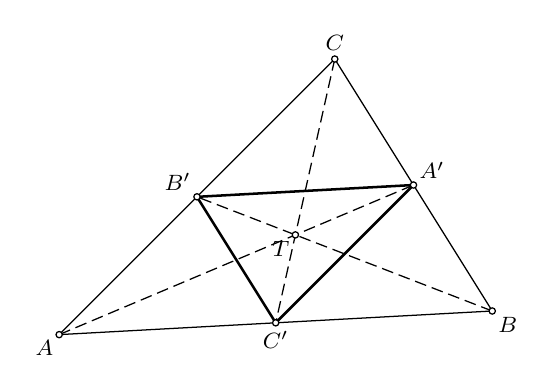
\begin{tikzpicture}
                % \clip (0,0) rectangle (14.000000,10.000000);
                {\footnotesize
                
                % Drawing segment A B
                \draw [line width=0.016cm] (1.539941,1.502179) -- (4.210059,1.647821);%
                \draw [line width=0.016cm] (4.289941,1.652179) -- (6.960059,1.797821);%
                
                % Drawing segment A C
                \draw [line width=0.016cm] (1.528284,1.528284) -- (3.221716,3.221716);%
                \draw [line width=0.016cm] (3.278284,3.278284) -- (4.971716,4.971716);%
                
                % Drawing segment B C
                \draw [line width=0.016cm] (6.978800,1.833920) -- (6.021200,3.366080);%
                \draw [line width=0.016cm] (5.978800,3.433920) -- (5.021200,4.966080);%
                
                % Drawing segment A A'
                \draw [line width=0.016cm] (1.536850,1.515559) -- (1.638187,1.558346);%
                \draw [line width=0.016cm] (1.707281,1.587519) -- (1.845469,1.645865);%
                \draw [line width=0.016cm] (1.914562,1.675037) -- (2.052750,1.733383);%
                \draw [line width=0.016cm] (2.121843,1.762556) -- (2.260031,1.820902);%
                \draw [line width=0.016cm] (2.329125,1.850075) -- (2.467312,1.908421);%
                \draw [line width=0.016cm] (2.536406,1.937594) -- (2.674593,1.995939);%
                \draw [line width=0.016cm] (2.743687,2.025112) -- (2.881874,2.083458);%
                \draw [line width=0.016cm] (2.950968,2.112631) -- (3.089155,2.170977);%
                \draw [line width=0.016cm] (3.158249,2.200150) -- (3.296437,2.258495);%
                \draw [line width=0.016cm] (3.365530,2.287668) -- (3.503718,2.346014);%
                \draw [line width=0.016cm] (3.572812,2.375187) -- (3.710999,2.433533);%
                \draw [line width=0.016cm] (3.780093,2.462706) -- (3.918280,2.521052);%
                \draw [line width=0.016cm] (3.987374,2.550225) -- (4.125561,2.608570);%
                \draw [line width=0.016cm] (4.194655,2.637743) -- (4.332842,2.696089);%
                \draw [line width=0.016cm] (4.401936,2.725262) -- (4.463150,2.751108);%
                \draw [line width=0.016cm] (4.536850,2.782226) -- (4.540124,2.783608);%
                \draw [line width=0.016cm] (4.609217,2.812781) -- (4.747405,2.871126);%
                \draw [line width=0.016cm] (4.816498,2.900299) -- (4.954686,2.958645);%
                \draw [line width=0.016cm] (5.023780,2.987818) -- (5.161967,3.046164);%
                \draw [line width=0.016cm] (5.231061,3.075337) -- (5.369248,3.133683);%
                \draw [line width=0.016cm] (5.438342,3.162855) -- (5.576529,3.221201);%
                \draw [line width=0.016cm] (5.645623,3.250374) -- (5.783810,3.308720);%
                \draw [line width=0.016cm] (5.852904,3.337893) -- (5.963150,3.384441);%
                
                % Drawing segment B B'
                \draw [line width=0.016cm] (6.962692,1.814426) -- (6.860095,1.854097);%
                \draw [line width=0.016cm] (6.790142,1.881145) -- (6.650236,1.935242);%
                \draw [line width=0.016cm] (6.580284,1.962290) -- (6.440378,2.016387);%
                \draw [line width=0.016cm] (6.370425,2.043436) -- (6.230520,2.097532);%
                \draw [line width=0.016cm] (6.160567,2.124581) -- (6.020662,2.178677);%
                \draw [line width=0.016cm] (5.950709,2.205726) -- (5.810804,2.259823);%
                \draw [line width=0.016cm] (5.740851,2.286871) -- (5.600945,2.340968);%
                \draw [line width=0.016cm] (5.530993,2.368016) -- (5.391087,2.422113);%
                \draw [line width=0.016cm] (5.321134,2.449161) -- (5.181229,2.503258);%
                \draw [line width=0.016cm] (5.111276,2.530307) -- (4.971371,2.584403);%
                \draw [line width=0.016cm] (4.901418,2.611452) -- (4.761513,2.665548);%
                \draw [line width=0.016cm] (4.691560,2.692597) -- (4.551654,2.746694);%
                \draw [line width=0.016cm] (4.462692,2.781092) -- (4.341796,2.827839);%
                \draw [line width=0.016cm] (4.271843,2.854887) -- (4.131938,2.908984);%
                \draw [line width=0.016cm] (4.061985,2.936032) -- (3.922080,2.990129);%
                \draw [line width=0.016cm] (3.852127,3.017178) -- (3.712222,3.071274);%
                \draw [line width=0.016cm] (3.642269,3.098323) -- (3.502363,3.152419);%
                \draw [line width=0.016cm] (3.432411,3.179468) -- (3.292505,3.233565);%
                
                % Drawing segment C C'
                \draw [line width=0.016cm] (4.991261,4.960966) -- (4.967229,4.853624);%
                \draw [line width=0.016cm] (4.950844,4.780435) -- (4.918073,4.634059);%
                \draw [line width=0.016cm] (4.901687,4.560871) -- (4.868917,4.414494);%
                \draw [line width=0.016cm] (4.852531,4.341306) -- (4.819760,4.194929);%
                \draw [line width=0.016cm] (4.803375,4.121741) -- (4.770604,3.975365);%
                \draw [line width=0.016cm] (4.754219,3.902176) -- (4.721448,3.755800);%
                \draw [line width=0.016cm] (4.705062,3.682612) -- (4.672291,3.536235);%
                \draw [line width=0.016cm] (4.655906,3.463047) -- (4.623135,3.316671);%
                \draw [line width=0.016cm] (4.606750,3.243482) -- (4.573979,3.097106);%
                \draw [line width=0.016cm] (4.557594,3.023918) -- (4.524823,2.877541);%
                \draw [line width=0.016cm] (4.491261,2.727633) -- (4.475666,2.657976);%
                \draw [line width=0.016cm] (4.459281,2.584788) -- (4.426510,2.438412);%
                \draw [line width=0.016cm] (4.410125,2.365224) -- (4.377354,2.218847);%
                \draw [line width=0.016cm] (4.360968,2.145659) -- (4.328198,1.999282);%
                \draw [line width=0.016cm] (4.311812,1.926094) -- (4.279041,1.779718);%
                \draw [line width=0.016cm] (4.262656,1.706529) -- (4.258739,1.689034);%
                
                % Marking point A by circle
                \draw [line width=0.016cm] (1.500000,1.500000) circle (0.040000);%
                \draw (1.530000,1.530000) node [anchor=north east] { $A$ };%
                
                % Marking point B by circle
                \draw [line width=0.016cm] (7.000000,1.800000) circle (0.040000);%
                \draw (6.970000,1.830000) node [anchor=north west] { $B$ };%
                
                % Marking point C by circle
                \draw [line width=0.016cm] (5.000000,5.000000) circle (0.040000);%
                \draw (5.000000,5.000000) node [anchor=south] { $C$ };%
                
                % Marking point A' by circle
                \draw [line width=0.016cm] (6.000000,3.400000) circle (0.040000);%
                \draw (5.970000,3.370000) node [anchor=south west] { $A'$ };%
                
                % Marking point B' by circle
                \draw [line width=0.016cm] (3.250000,3.250000) circle (0.040000);%
                \draw (3.280000,3.220000) node [anchor=south east] { $B'$ };%
                
                % Marking point C' by circle
                \draw [line width=0.016cm] (4.250000,1.650000) circle (0.040000);%
                \draw (4.250000,1.650000) node [anchor=north] { $C'$ };%
                
                % Marking point T by circle
                \draw [line width=0.016cm] (4.500000,2.766667) circle (0.040000);%
                \draw (4.530000,2.796667) node [anchor=north east] { $T$ };%
                
                % Drawing segment A' B'
                \draw [line width=0.032cm] (5.960059,3.397821) -- (3.289941,3.252179);%
                
                % Drawing segment B' C'
                \draw [line width=0.032cm] (3.271200,3.216080) -- (4.228800,1.683920);%
                
                % Drawing segment A' C'
                \draw [line width=0.032cm] (5.971716,3.371716) -- (4.278284,1.678284);%
                }
            \end{tikzpicture}

        \begin{opomba}
            Trikotnik $\triangle A'B'C'$ je podoben osnovnemu trikotniku $\triangle ABC$, saj so ustrezne stranice vzporedne. Faktor podobnosti je $\frac{1}{2}$, bolj natančno je ta podobnost dana z raztegom s središčem $T$ in faktorjem $-\frac{1}{2}$, kjer $-$ pomeni, da točko zrcalimo preko točke $T$. To transformacijo zapišemo kot $R(T,-\frac{1}{2})$.
        \end{opomba}

    \subsection*{Včrtane krožnice in pričrtane krožnice}

        Za trikotnik $\triangle ABC$ je središče $I$ njegove \textbf{včrtane krožnice} enako preseku simetral notranjih kotov trikotnika.
        
            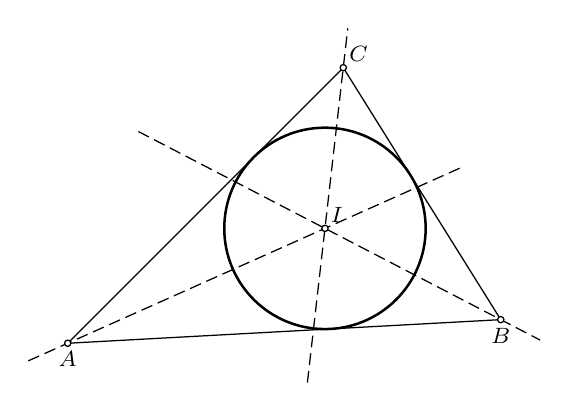
\begin{tikzpicture}
                % \clip (0,0) rectangle (14.000000,10.000000);
                {\footnotesize
                
                % Drawing segment A B
                \draw [line width=0.016cm] (1.539941,1.502179) -- (6.960059,1.797821);%
                
                % Drawing segment A C
                \draw [line width=0.016cm] (1.528284,1.528284) -- (4.971716,4.971716);%
                
                % Drawing segment B C
                \draw [line width=0.016cm] (6.978800,1.833920) -- (5.021200,4.966080);%
                
                % Drawing line a
                \draw [line width=0.016cm] (1.000000,1.276747) -- (1.136967,1.337903);%
                \draw [line width=0.016cm] (1.205450,1.368482) -- (1.342417,1.429638);%
                \draw [line width=0.016cm] (1.410900,1.460216) -- (1.463476,1.483692);%
                \draw [line width=0.016cm] (1.536524,1.516308) -- (1.547867,1.521373);%
                \draw [line width=0.016cm] (1.616350,1.551951) -- (1.753317,1.613108);%
                \draw [line width=0.016cm] (1.821800,1.643686) -- (1.958767,1.704842);%
                \draw [line width=0.016cm] (2.027250,1.735421) -- (2.164217,1.796577);%
                \draw [line width=0.016cm] (2.232700,1.827155) -- (2.369667,1.888312);%
                \draw [line width=0.016cm] (2.438151,1.918890) -- (2.575117,1.980047);%
                \draw [line width=0.016cm] (2.643601,2.010625) -- (2.780567,2.071781);%
                \draw [line width=0.016cm] (2.849051,2.102360) -- (2.986017,2.163516);%
                \draw [line width=0.016cm] (3.054501,2.194094) -- (3.191467,2.255251);%
                \draw [line width=0.016cm] (3.259951,2.285829) -- (3.396918,2.346986);%
                \draw [line width=0.016cm] (3.465401,2.377564) -- (3.602368,2.438720);%
                \draw [line width=0.016cm] (3.670851,2.469299) -- (3.807818,2.530455);%
                \draw [line width=0.016cm] (3.876301,2.561034) -- (4.013268,2.622190);%
                \draw [line width=0.016cm] (4.081751,2.652768) -- (4.218718,2.713925);%
                \draw [line width=0.016cm] (4.287201,2.744503) -- (4.424168,2.805660);%
                \draw [line width=0.016cm] (4.492651,2.836238) -- (4.629618,2.897394);%
                \draw [line width=0.016cm] (4.698101,2.927973) -- (4.731028,2.942675);%
                \draw [line width=0.016cm] (4.804077,2.975291) -- (4.835068,2.989129);%
                \draw [line width=0.016cm] (4.903551,3.019707) -- (5.040518,3.080864);%
                \draw [line width=0.016cm] (5.109001,3.111442) -- (5.245968,3.172599);%
                \draw [line width=0.016cm] (5.314452,3.203177) -- (5.451418,3.264333);%
                \draw [line width=0.016cm] (5.519902,3.294912) -- (5.656868,3.356068);%
                \draw [line width=0.016cm] (5.725352,3.386646) -- (5.862318,3.447803);%
                \draw [line width=0.016cm] (5.930802,3.478381) -- (6.067769,3.539538);%
                \draw [line width=0.016cm] (6.136252,3.570116) -- (6.273219,3.631272);%
                \draw [line width=0.016cm] (6.341702,3.661851) -- (6.478669,3.723007);%
                
                % Drawing line b
                \draw [line width=0.016cm] (2.397850,4.189222) -- (2.530979,4.120108);%
                \draw [line width=0.016cm] (2.597543,4.085551) -- (2.730672,4.016437);%
                \draw [line width=0.016cm] (2.797236,3.981880) -- (2.930365,3.912766);%
                \draw [line width=0.016cm] (2.996929,3.878208) -- (3.130058,3.809094);%
                \draw [line width=0.016cm] (3.196622,3.774537) -- (3.329751,3.705423);%
                \draw [line width=0.016cm] (3.396315,3.670866) -- (3.529444,3.601752);%
                \draw [line width=0.016cm] (3.596008,3.567195) -- (3.729137,3.498080);%
                \draw [line width=0.016cm] (3.795701,3.463523) -- (3.928830,3.394409);%
                \draw [line width=0.016cm] (3.995394,3.359852) -- (4.128522,3.290738);%
                \draw [line width=0.016cm] (4.195087,3.256181) -- (4.328215,3.187066);%
                \draw [line width=0.016cm] (4.394780,3.152509) -- (4.527908,3.083395);%
                \draw [line width=0.016cm] (4.594473,3.048838) -- (4.727601,2.979724);%
                \draw [line width=0.016cm] (4.803054,2.940553) -- (4.927294,2.876053);%
                \draw [line width=0.016cm] (4.993858,2.841496) -- (5.126987,2.772381);%
                \draw [line width=0.016cm] (5.193551,2.737824) -- (5.326680,2.668710);%
                \draw [line width=0.016cm] (5.393244,2.634153) -- (5.526373,2.565039);%
                \draw [line width=0.016cm] (5.592937,2.530482) -- (5.726066,2.461367);%
                \draw [line width=0.016cm] (5.792630,2.426810) -- (5.925759,2.357696);%
                \draw [line width=0.016cm] (5.992323,2.323139) -- (6.125452,2.254025);%
                \draw [line width=0.016cm] (6.192016,2.219468) -- (6.325145,2.150354);%
                \draw [line width=0.016cm] (6.391709,2.115796) -- (6.524838,2.046682);%
                \draw [line width=0.016cm] (6.591402,2.012125) -- (6.724530,1.943011);%
                \draw [line width=0.016cm] (6.791095,1.908454) -- (6.924223,1.839340);%
                \draw [line width=0.016cm] (7.035501,1.781570) -- (7.123916,1.735668);%
                \draw [line width=0.016cm] (7.190481,1.701111) -- (7.323609,1.631997);%
                \draw [line width=0.016cm] (7.390174,1.597440) -- (7.500000,1.540423);%
                
                % Drawing line c
                \draw [line width=0.016cm] (4.544448,1.000000) -- (4.561421,1.149037);%
                \draw [line width=0.016cm] (4.569908,1.223555) -- (4.586882,1.372591);%
                \draw [line width=0.016cm] (4.595368,1.447110) -- (4.612342,1.596146);%
                \draw [line width=0.016cm] (4.620829,1.670665) -- (4.637802,1.819701);%
                \draw [line width=0.016cm] (4.646289,1.894219) -- (4.663262,2.043256);%
                \draw [line width=0.016cm] (4.671749,2.117774) -- (4.688723,2.266811);%
                \draw [line width=0.016cm] (4.697209,2.341329) -- (4.714183,2.490366);%
                \draw [line width=0.016cm] (4.722669,2.564884) -- (4.739643,2.713921);%
                \draw [line width=0.016cm] (4.748130,2.788439) -- (4.763026,2.919240);%
                \draw [line width=0.016cm] (4.773590,3.011994) -- (4.790563,3.161030);%
                \draw [line width=0.016cm] (4.799050,3.235549) -- (4.816024,3.384585);%
                \draw [line width=0.016cm] (4.824510,3.459104) -- (4.841484,3.608140);%
                \draw [line width=0.016cm] (4.849971,3.682658) -- (4.866944,3.831695);%
                \draw [line width=0.016cm] (4.875431,3.906213) -- (4.892404,4.055250);%
                \draw [line width=0.016cm] (4.900891,4.129768) -- (4.917864,4.278805);%
                \draw [line width=0.016cm] (4.926351,4.353323) -- (4.943325,4.502360);%
                \draw [line width=0.016cm] (4.951811,4.576878) -- (4.968785,4.725914);%
                \draw [line width=0.016cm] (4.977272,4.800433) -- (4.994245,4.949469);%
                \draw [line width=0.016cm] (5.004526,5.039743) -- (5.019705,5.173024);%
                \draw [line width=0.016cm] (5.028192,5.247542) -- (5.045166,5.396579);%
                \draw [line width=0.016cm] (5.053652,5.471097) -- (5.056944,5.500000);%
                
                % Marking point A by circle
                \draw [line width=0.016cm] (1.500000,1.500000) circle (0.040000);%
                \draw (1.500000,1.500000) node [anchor=north] { $A$ };%
                
                % Marking point B by circle
                \draw [line width=0.016cm] (7.000000,1.800000) circle (0.040000);%
                \draw (7.000000,1.800000) node [anchor=north] { $B$ };%
                
                % Marking point C by circle
                \draw [line width=0.016cm] (5.000000,5.000000) circle (0.040000);%
                \draw (4.970000,4.970000) node [anchor=south west] { $C$ };%
                
                % Marking point I by circle
                \draw [line width=0.016cm] (4.767553,2.958983) circle (0.040000);%
                \draw (4.737553,2.928983) node [anchor=south west] { $I$ };%
                
                % Drawing circle I P
                \draw [line width=0.032cm] (4.767553,2.958983) circle (1.278852);%
                }
            \end{tikzpicture}
            
        \noindent Naj bo $I_a$ presek simetrale notranjega kota pri $A$ in zunanjega kota pri $B$. Točka $I_a$ je enako oddaljena od $\overleftrightarrow{AB}$ in $\overleftrightarrow{AC}$ ter enako oddaljena od $\overleftrightarrow{AB}$ in $\overleftrightarrow{BC}$, zato je tudi enako oddaljena od $\overleftrightarrow{AC}$ in $\overleftrightarrow{BC}$, torej leži tudi na simetrali zunanjega kota pri $C$. Zato je točka $I_a$ središče \textbf{pričrtane krožnice} k trikotniku $\triangle ABC$, ki se dotika stranice $a$ ($=BC$) in nosilk drugih dveh stranic.

            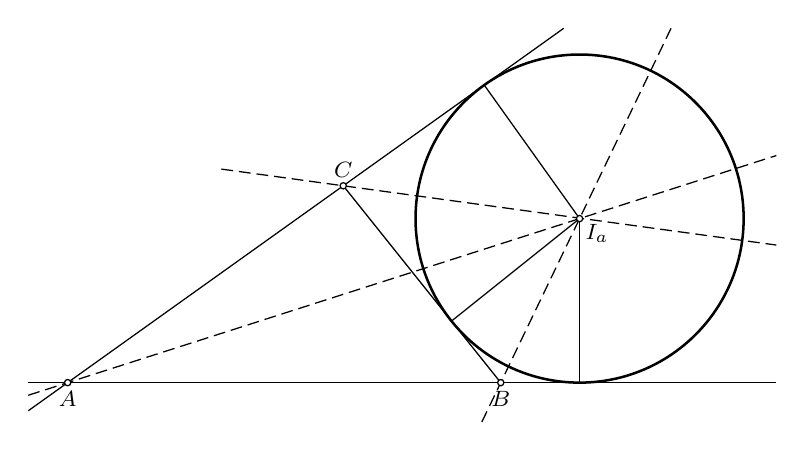
\begin{tikzpicture}
                % \clip (0,0) rectangle (14.000000,10.000000);
                {\footnotesize
                
                % Drawing line A B
                \draw [line width=0.016cm] (1.000000,1.500000) -- (1.460000,1.500000);%
                \draw [line width=0.016cm] (1.540000,1.500000) -- (6.960000,1.500000);%
                \draw [line width=0.016cm] (7.040000,1.500000) -- (10.500000,1.500000);%
                
                % Drawing line A C
                \draw [line width=0.016cm] (7.800000,6.000000) -- (5.032549,4.023250);%
                \draw [line width=0.016cm] (4.967451,3.976750) -- (1.532549,1.523250);%
                \draw [line width=0.016cm] (1.467451,1.476750) -- (1.000000,1.142857);%
                
                % Drawing segment B C
                \draw [line width=0.016cm] (6.975012,1.531235) -- (5.024988,3.968765);%
                
                % Drawing line a
                \draw [line width=0.016cm] (1.000000,1.339767) -- (1.142844,1.385544);%
                \draw [line width=0.016cm] (1.214266,1.408432) -- (1.357111,1.454209);%
                \draw [line width=0.016cm] (1.428533,1.477097) -- (1.461908,1.487793);%
                \draw [line width=0.016cm] (1.538092,1.512207) -- (1.571377,1.522874);%
                \draw [line width=0.016cm] (1.642799,1.545762) -- (1.785644,1.591539);%
                \draw [line width=0.016cm] (1.857066,1.614427) -- (1.999910,1.660204);%
                \draw [line width=0.016cm] (2.071332,1.683092) -- (2.214177,1.728869);%
                \draw [line width=0.016cm] (2.285599,1.751757) -- (2.428443,1.797534);%
                \draw [line width=0.016cm] (2.499865,1.820422) -- (2.642710,1.866199);%
                \draw [line width=0.016cm] (2.714132,1.889087) -- (2.856976,1.934863);%
                \draw [line width=0.016cm] (2.928398,1.957752) -- (3.071243,2.003528);%
                \draw [line width=0.016cm] (3.142665,2.026417) -- (3.285509,2.072193);%
                \draw [line width=0.016cm] (3.356931,2.095082) -- (3.499776,2.140858);%
                \draw [line width=0.016cm] (3.571198,2.163747) -- (3.714042,2.209523);%
                \draw [line width=0.016cm] (3.785464,2.232411) -- (3.928309,2.278188);%
                \draw [line width=0.016cm] (3.999731,2.301076) -- (4.142575,2.346853);%
                \draw [line width=0.016cm] (4.213997,2.369741) -- (4.356842,2.415518);%
                \draw [line width=0.016cm] (4.428264,2.438406) -- (4.571108,2.484183);%
                \draw [line width=0.016cm] (4.642530,2.507071) -- (4.785375,2.552848);%
                \draw [line width=0.016cm] (4.856797,2.575736) -- (4.999641,2.621513);%
                \draw [line width=0.016cm] (5.071063,2.644401) -- (5.213908,2.690178);%
                \draw [line width=0.016cm] (5.285330,2.713066) -- (5.428174,2.758843);%
                \draw [line width=0.016cm] (5.499596,2.781731) -- (5.642441,2.827507);%
                \draw [line width=0.016cm] (5.713863,2.850396) -- (5.856707,2.896172);%
                \draw [line width=0.016cm] (5.928129,2.919061) -- (6.070974,2.964837);%
                \draw [line width=0.016cm] (6.142396,2.987726) -- (6.285240,3.033502);%
                \draw [line width=0.016cm] (6.356662,3.056391) -- (6.499507,3.102167);%
                \draw [line width=0.016cm] (6.570929,3.125055) -- (6.713773,3.170832);%
                \draw [line width=0.016cm] (6.785195,3.193720) -- (6.928040,3.239497);%
                \draw [line width=0.016cm] (6.999462,3.262385) -- (7.142306,3.308162);%
                \draw [line width=0.016cm] (7.213728,3.331050) -- (7.356573,3.376827);%
                \draw [line width=0.016cm] (7.427995,3.399715) -- (7.570839,3.445492);%
                \draw [line width=0.016cm] (7.642261,3.468380) -- (7.785105,3.514157);%
                \draw [line width=0.016cm] (7.856528,3.537045) -- (7.963271,3.571252);%
                \draw [line width=0.016cm] (8.070794,3.605710) -- (8.213638,3.651487);%
                \draw [line width=0.016cm] (8.285061,3.674375) -- (8.427905,3.720151);%
                \draw [line width=0.016cm] (8.499327,3.743040) -- (8.642171,3.788816);%
                \draw [line width=0.016cm] (8.713594,3.811705) -- (8.856438,3.857481);%
                \draw [line width=0.016cm] (8.927860,3.880370) -- (9.070704,3.926146);%
                \draw [line width=0.016cm] (9.142127,3.949035) -- (9.284971,3.994811);%
                \draw [line width=0.016cm] (9.356393,4.017699) -- (9.499237,4.063476);%
                \draw [line width=0.016cm] (9.570660,4.086364) -- (9.713504,4.132141);%
                \draw [line width=0.016cm] (9.784926,4.155029) -- (9.927770,4.200806);%
                \draw [line width=0.016cm] (9.999193,4.223694) -- (10.142037,4.269471);%
                \draw [line width=0.016cm] (10.213459,4.292359) -- (10.356303,4.338136);%
                \draw [line width=0.016cm] (10.427726,4.361024) -- (10.500000,4.384185);%
                
                % Drawing line b
                \draw [line width=0.016cm] (6.759688,1.000000) -- (6.824666,1.135195);%
                \draw [line width=0.016cm] (6.857155,1.202793) -- (6.922133,1.337989);%
                \draw [line width=0.016cm] (6.954623,1.405586) -- (6.982672,1.463948);%
                \draw [line width=0.016cm] (7.017328,1.536052) -- (7.019601,1.540782);%
                \draw [line width=0.016cm] (7.052090,1.608380) -- (7.117068,1.743575);%
                \draw [line width=0.016cm] (7.149557,1.811173) -- (7.214536,1.946368);%
                \draw [line width=0.016cm] (7.247025,2.013966) -- (7.312003,2.149162);%
                \draw [line width=0.016cm] (7.344492,2.216759) -- (7.409471,2.351955);%
                \draw [line width=0.016cm] (7.441960,2.419553) -- (7.506938,2.554748);%
                \draw [line width=0.016cm] (7.539427,2.622346) -- (7.604406,2.757541);%
                \draw [line width=0.016cm] (7.636895,2.825139) -- (7.701873,2.960335);%
                \draw [line width=0.016cm] (7.734362,3.027932) -- (7.799341,3.163128);%
                \draw [line width=0.016cm] (7.831830,3.230726) -- (7.896808,3.365921);%
                \draw [line width=0.016cm] (7.929297,3.433519) -- (7.984035,3.547407);%
                \draw [line width=0.016cm] (8.026765,3.636312) -- (8.091743,3.771507);%
                \draw [line width=0.016cm] (8.124232,3.839105) -- (8.189210,3.974301);%
                \draw [line width=0.016cm] (8.221700,4.041898) -- (8.286678,4.177094);%
                \draw [line width=0.016cm] (8.319167,4.244692) -- (8.384145,4.379887);%
                \draw [line width=0.016cm] (8.416634,4.447485) -- (8.481613,4.582680);%
                \draw [line width=0.016cm] (8.514102,4.650278) -- (8.579080,4.785474);%
                \draw [line width=0.016cm] (8.611569,4.853071) -- (8.676548,4.988267);%
                \draw [line width=0.016cm] (8.709037,5.055865) -- (8.774015,5.191060);%
                \draw [line width=0.016cm] (8.806504,5.258658) -- (8.871483,5.393853);%
                \draw [line width=0.016cm] (8.903972,5.461451) -- (8.968950,5.596647);%
                \draw [line width=0.016cm] (9.001439,5.664244) -- (9.066418,5.799440);%
                \draw [line width=0.016cm] (9.098907,5.867037) -- (9.162812,6.000000);%
                
                % Drawing line c
                \draw [line width=0.016cm] (3.452141,4.211842) -- (3.600756,4.191502);%
                \draw [line width=0.016cm] (3.675063,4.181332) -- (3.823678,4.160993);%
                \draw [line width=0.016cm] (3.897985,4.150823) -- (4.046599,4.130484);%
                \draw [line width=0.016cm] (4.120907,4.120314) -- (4.269521,4.099974);%
                \draw [line width=0.016cm] (4.343829,4.089804) -- (4.492443,4.069465);%
                \draw [line width=0.016cm] (4.566751,4.059295) -- (4.715365,4.038955);%
                \draw [line width=0.016cm] (4.789673,4.028786) -- (4.938287,4.008446);%
                \draw [line width=0.016cm] (5.039631,3.994576) -- (5.161209,3.977937);%
                \draw [line width=0.016cm] (5.235516,3.967767) -- (5.384131,3.947427);%
                \draw [line width=0.016cm] (5.458438,3.937258) -- (5.607053,3.916918);%
                \draw [line width=0.016cm] (5.681360,3.906748) -- (5.829975,3.886409);%
                \draw [line width=0.016cm] (5.904282,3.876239) -- (6.052897,3.855899);%
                \draw [line width=0.016cm] (6.127204,3.845730) -- (6.275819,3.825390);%
                \draw [line width=0.016cm] (6.350126,3.815220) -- (6.498740,3.794881);%
                \draw [line width=0.016cm] (6.573048,3.784711) -- (6.721662,3.764371);%
                \draw [line width=0.016cm] (6.795970,3.754201) -- (6.944584,3.733862);%
                \draw [line width=0.016cm] (7.018892,3.723692) -- (7.167506,3.703352);%
                \draw [line width=0.016cm] (7.241814,3.693183) -- (7.390428,3.672843);%
                \draw [line width=0.016cm] (7.464735,3.662673) -- (7.613350,3.642334);%
                \draw [line width=0.016cm] (7.687657,3.632164) -- (7.836272,3.611824);%
                \draw [line width=0.016cm] (7.910579,3.601655) -- (7.962914,3.594492);%
                \draw [line width=0.016cm] (8.041361,3.583756) -- (8.059194,3.581315);%
                \draw [line width=0.016cm] (8.133501,3.571145) -- (8.282116,3.550806);%
                \draw [line width=0.016cm] (8.356423,3.540636) -- (8.505038,3.520296);%
                \draw [line width=0.016cm] (8.579345,3.510127) -- (8.727960,3.489787);%
                \draw [line width=0.016cm] (8.802267,3.479617) -- (8.950882,3.459278);%
                \draw [line width=0.016cm] (9.025189,3.449108) -- (9.173803,3.428768);%
                \draw [line width=0.016cm] (9.248111,3.418598) -- (9.396725,3.398259);%
                \draw [line width=0.016cm] (9.471033,3.388089) -- (9.619647,3.367750);%
                \draw [line width=0.016cm] (9.693955,3.357580) -- (9.842569,3.337240);%
                \draw [line width=0.016cm] (9.916876,3.327070) -- (10.065491,3.306731);%
                \draw [line width=0.016cm] (10.139798,3.296561) -- (10.288413,3.276221);%
                \draw [line width=0.016cm] (10.362720,3.266052) -- (10.500000,3.247263);%
                
                % Drawing segment I_a Q
                \draw [line width=0.016cm] (7.970128,3.558472) -- (6.374454,2.281933);%
                
                % Drawing segment I_a P
                \draw [line width=0.016cm] (8.001362,3.543459) -- (8.001362,1.500000);%
                
                % Drawing segment I_a R
                \draw [line width=0.016cm] (7.978113,3.616009) -- (6.790376,5.278840);%
                
                % Marking point A by circle
                \draw [line width=0.016cm] (1.500000,1.500000) circle (0.040000);%
                \draw (1.500000,1.500000) node [anchor=north] { $A$ };%
                
                % Marking point B by circle
                \draw [line width=0.016cm] (7.000000,1.500000) circle (0.040000);%
                \draw (7.000000,1.500000) node [anchor=north] { $B$ };%
                
                % Marking point C by circle
                \draw [line width=0.016cm] (5.000000,4.000000) circle (0.040000);%
                \draw (5.000000,4.000000) node [anchor=south] { $C$ };%
                
                % Marking point I_a by circle
                \draw [line width=0.016cm] (8.001362,3.583459) circle (0.040000);%
                \draw (7.971362,3.613459) node [anchor=north west] { $I_a$ };%
                
                % Drawing circle I_a P
                \draw [line width=0.032cm] (8.001362,3.583459) circle (2.083459);%
                }
            \end{tikzpicture}            

        \noindent Podobno dobimo še točki $I_b$ in $I_c$, ki sta središči drugih dveh pričrtanih krožnic.

        \paragraph{}
        Povezave med ploščino $p$ trikotnika $\triangle ABC$ in polmerom $r$ včrtane krožnice in polmeri $r_a,~r_b,~r_c$ pričrtanih krožnic:

            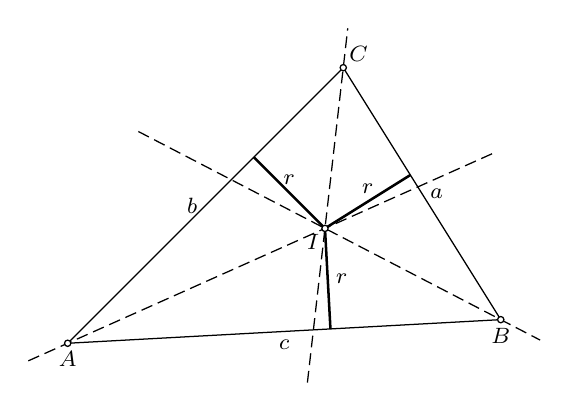
\begin{tikzpicture}
                % \clip (0,0) rectangle (14.000000,10.000000);
                {\footnotesize
                
                % Drawing segment A B
                \draw [line width=0.016cm] (1.539941,1.502179) -- (6.960059,1.797821);%
                
                % Drawing segment A C
                \draw [line width=0.016cm] (1.528284,1.528284) -- (4.971716,4.971716);%
                
                % Drawing segment B C
                \draw [line width=0.016cm] (6.978800,1.833920) -- (5.021200,4.966080);%
                
                % Drawing line a
                \draw [line width=0.016cm] (1.000000,1.276747) -- (1.136967,1.337903);%
                \draw [line width=0.016cm] (1.205450,1.368482) -- (1.342417,1.429638);%
                \draw [line width=0.016cm] (1.410900,1.460216) -- (1.463476,1.483692);%
                \draw [line width=0.016cm] (1.536524,1.516308) -- (1.547867,1.521373);%
                \draw [line width=0.016cm] (1.616350,1.551951) -- (1.753317,1.613108);%
                \draw [line width=0.016cm] (1.821800,1.643686) -- (1.958767,1.704842);%
                \draw [line width=0.016cm] (2.027250,1.735421) -- (2.164217,1.796577);%
                \draw [line width=0.016cm] (2.232700,1.827155) -- (2.369667,1.888312);%
                \draw [line width=0.016cm] (2.438151,1.918890) -- (2.575117,1.980047);%
                \draw [line width=0.016cm] (2.643601,2.010625) -- (2.780567,2.071781);%
                \draw [line width=0.016cm] (2.849051,2.102360) -- (2.986017,2.163516);%
                \draw [line width=0.016cm] (3.054501,2.194094) -- (3.191467,2.255251);%
                \draw [line width=0.016cm] (3.259951,2.285829) -- (3.396918,2.346986);%
                \draw [line width=0.016cm] (3.465401,2.377564) -- (3.602368,2.438720);%
                \draw [line width=0.016cm] (3.670851,2.469299) -- (3.807818,2.530455);%
                \draw [line width=0.016cm] (3.876301,2.561034) -- (4.013268,2.622190);%
                \draw [line width=0.016cm] (4.081751,2.652768) -- (4.218718,2.713925);%
                \draw [line width=0.016cm] (4.287201,2.744503) -- (4.424168,2.805660);%
                \draw [line width=0.016cm] (4.492651,2.836238) -- (4.629618,2.897394);%
                \draw [line width=0.016cm] (4.698101,2.927973) -- (4.731028,2.942675);%
                \draw [line width=0.016cm] (4.804077,2.975291) -- (4.835068,2.989129);%
                \draw [line width=0.016cm] (4.903551,3.019707) -- (5.040518,3.080864);%
                \draw [line width=0.016cm] (5.109001,3.111442) -- (5.245968,3.172599);%
                \draw [line width=0.016cm] (5.314452,3.203177) -- (5.451418,3.264333);%
                \draw [line width=0.016cm] (5.519902,3.294912) -- (5.656868,3.356068);%
                \draw [line width=0.016cm] (5.725352,3.386646) -- (5.862318,3.447803);%
                \draw [line width=0.016cm] (5.930802,3.478381) -- (6.067769,3.539538);%
                \draw [line width=0.016cm] (6.136252,3.570116) -- (6.273219,3.631272);%
                \draw [line width=0.016cm] (6.341702,3.661851) -- (6.478669,3.723007);%
                \draw [line width=0.016cm] (6.547152,3.753585) -- (6.684119,3.814742);%
                \draw [line width=0.016cm] (6.752602,3.845320) -- (6.889569,3.906477);%
                
                % Drawing line b
                \draw [line width=0.016cm] (2.397850,4.189222) -- (2.530979,4.120108);%
                \draw [line width=0.016cm] (2.597543,4.085551) -- (2.730672,4.016437);%
                \draw [line width=0.016cm] (2.797236,3.981880) -- (2.930365,3.912766);%
                \draw [line width=0.016cm] (2.996929,3.878208) -- (3.130058,3.809094);%
                \draw [line width=0.016cm] (3.196622,3.774537) -- (3.329751,3.705423);%
                \draw [line width=0.016cm] (3.396315,3.670866) -- (3.529444,3.601752);%
                \draw [line width=0.016cm] (3.596008,3.567195) -- (3.729137,3.498080);%
                \draw [line width=0.016cm] (3.795701,3.463523) -- (3.928830,3.394409);%
                \draw [line width=0.016cm] (3.995394,3.359852) -- (4.128522,3.290738);%
                \draw [line width=0.016cm] (4.195087,3.256181) -- (4.328215,3.187066);%
                \draw [line width=0.016cm] (4.394780,3.152509) -- (4.527908,3.083395);%
                \draw [line width=0.016cm] (4.594473,3.048838) -- (4.727601,2.979724);%
                \draw [line width=0.016cm] (4.803054,2.940553) -- (4.927294,2.876053);%
                \draw [line width=0.016cm] (4.993858,2.841496) -- (5.126987,2.772381);%
                \draw [line width=0.016cm] (5.193551,2.737824) -- (5.326680,2.668710);%
                \draw [line width=0.016cm] (5.393244,2.634153) -- (5.526373,2.565039);%
                \draw [line width=0.016cm] (5.592937,2.530482) -- (5.726066,2.461367);%
                \draw [line width=0.016cm] (5.792630,2.426810) -- (5.925759,2.357696);%
                \draw [line width=0.016cm] (5.992323,2.323139) -- (6.125452,2.254025);%
                \draw [line width=0.016cm] (6.192016,2.219468) -- (6.325145,2.150354);%
                \draw [line width=0.016cm] (6.391709,2.115796) -- (6.524838,2.046682);%
                \draw [line width=0.016cm] (6.591402,2.012125) -- (6.724530,1.943011);%
                \draw [line width=0.016cm] (6.791095,1.908454) -- (6.924223,1.839340);%
                \draw [line width=0.016cm] (7.035501,1.781570) -- (7.123916,1.735668);%
                \draw [line width=0.016cm] (7.190481,1.701111) -- (7.323609,1.631997);%
                \draw [line width=0.016cm] (7.390174,1.597440) -- (7.500000,1.540423);%
                
                % Drawing line c
                \draw [line width=0.016cm] (4.544448,1.000000) -- (4.561421,1.149037);%
                \draw [line width=0.016cm] (4.569908,1.223555) -- (4.586882,1.372591);%
                \draw [line width=0.016cm] (4.595368,1.447110) -- (4.612342,1.596146);%
                \draw [line width=0.016cm] (4.620829,1.670665) -- (4.637802,1.819701);%
                \draw [line width=0.016cm] (4.646289,1.894219) -- (4.663262,2.043256);%
                \draw [line width=0.016cm] (4.671749,2.117774) -- (4.688723,2.266811);%
                \draw [line width=0.016cm] (4.697209,2.341329) -- (4.714183,2.490366);%
                \draw [line width=0.016cm] (4.722669,2.564884) -- (4.739643,2.713921);%
                \draw [line width=0.016cm] (4.748130,2.788439) -- (4.763026,2.919240);%
                \draw [line width=0.016cm] (4.773590,3.011994) -- (4.790563,3.161030);%
                \draw [line width=0.016cm] (4.799050,3.235549) -- (4.816024,3.384585);%
                \draw [line width=0.016cm] (4.824510,3.459104) -- (4.841484,3.608140);%
                \draw [line width=0.016cm] (4.849971,3.682658) -- (4.866944,3.831695);%
                \draw [line width=0.016cm] (4.875431,3.906213) -- (4.892404,4.055250);%
                \draw [line width=0.016cm] (4.900891,4.129768) -- (4.917864,4.278805);%
                \draw [line width=0.016cm] (4.926351,4.353323) -- (4.943325,4.502360);%
                \draw [line width=0.016cm] (4.951811,4.576878) -- (4.968785,4.725914);%
                \draw [line width=0.016cm] (4.977272,4.800433) -- (4.994245,4.949469);%
                \draw [line width=0.016cm] (5.004526,5.039743) -- (5.019705,5.173024);%
                \draw [line width=0.016cm] (5.028192,5.247542) -- (5.045166,5.396579);%
                \draw [line width=0.016cm] (5.053652,5.471097) -- (5.056944,5.500000);%
                
                % Marking point A by circle
                \draw [line width=0.016cm] (1.500000,1.500000) circle (0.040000);%
                \draw (1.500000,1.500000) node [anchor=north] { $A$ };%
                
                % Marking point B by circle
                \draw [line width=0.016cm] (7.000000,1.800000) circle (0.040000);%
                \draw (7.000000,1.800000) node [anchor=north] { $B$ };%
                
                % Marking point C by circle
                \draw [line width=0.016cm] (5.000000,5.000000) circle (0.040000);%
                \draw (4.970000,4.970000) node [anchor=south west] { $C$ };%
                
                % Marking point I by circle
                \draw [line width=0.016cm] (4.767553,2.958983) circle (0.040000);%
                \draw (4.797553,2.988983) node [anchor=north east] { $I$ };%
                
                % Marking point r
                \draw (4.315410,3.411125) node [anchor=south] { $r$ };%
                
                % Marking point r
                \draw (4.802379,2.320506) node [anchor=west] { $r$ };%
                
                % Marking point r
                \draw (5.309785,3.297878) node [anchor=south] { $r$ };%
                
                % Marking point a
                \draw (6.000000,3.400000) node [anchor=west] { $a$ };%
                
                % Marking point c
                \draw (4.250000,1.650000) node [anchor=north] { $c$ };%
                
                % Marking point b
                \draw (3.250000,3.250000) node [anchor=east] { $b$ };%
                
                % Drawing segment I K
                \draw [line width=0.032cm] (4.769731,2.919042) -- (4.837205,1.682029);%
                
                % Drawing segment I L
                \draw [line width=0.032cm] (4.801473,2.980183) -- (5.852017,3.636773);%
                
                % Drawing segment I M
                \draw [line width=0.032cm] (4.739268,2.987267) -- (3.863268,3.863268);%
                }
            \end{tikzpicture}            

        $p=\frac{a\cdot r}{2}+\frac{b\cdot r}{2}+\frac{c\cdot r}{2}=r(\frac{a+b+c}{2})=r\cdot s$, kjer je $s=\frac{a+b+c}{2}$

            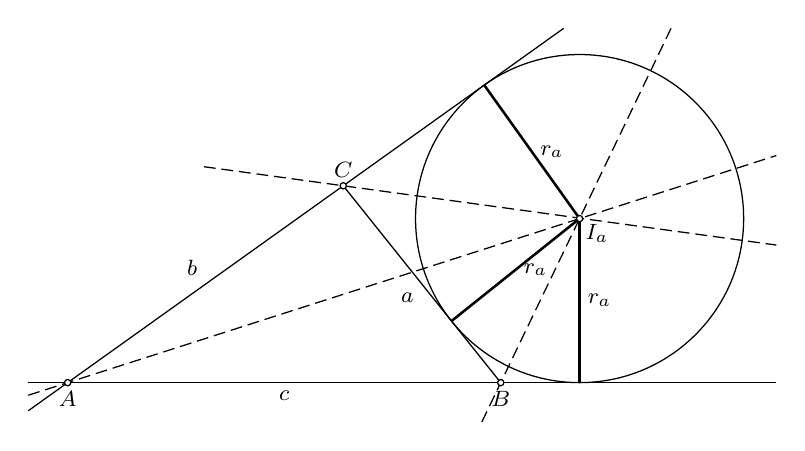
\begin{tikzpicture}
                % \clip (0,0) rectangle (14.000000,10.000000);
                {\footnotesize
                
                % Drawing line A B
                \draw [line width=0.016cm] (1.000000,1.500000) -- (1.460000,1.500000);%
                \draw [line width=0.016cm] (1.540000,1.500000) -- (6.960000,1.500000);%
                \draw [line width=0.016cm] (7.040000,1.500000) -- (10.500000,1.500000);%
                
                % Drawing line A C
                \draw [line width=0.016cm] (7.800000,6.000000) -- (5.032549,4.023250);%
                \draw [line width=0.016cm] (4.967451,3.976750) -- (1.532549,1.523250);%
                \draw [line width=0.016cm] (1.467451,1.476750) -- (1.000000,1.142857);%
                
                % Drawing segment B C
                \draw [line width=0.016cm] (6.975012,1.531235) -- (5.024988,3.968765);%
                
                % Drawing line a
                \draw [line width=0.016cm] (1.000000,1.339767) -- (1.142844,1.385544);%
                \draw [line width=0.016cm] (1.214266,1.408432) -- (1.357111,1.454209);%
                \draw [line width=0.016cm] (1.428533,1.477097) -- (1.461908,1.487793);%
                \draw [line width=0.016cm] (1.538092,1.512207) -- (1.571377,1.522874);%
                \draw [line width=0.016cm] (1.642799,1.545762) -- (1.785644,1.591539);%
                \draw [line width=0.016cm] (1.857066,1.614427) -- (1.999910,1.660204);%
                \draw [line width=0.016cm] (2.071332,1.683092) -- (2.214177,1.728869);%
                \draw [line width=0.016cm] (2.285599,1.751757) -- (2.428443,1.797534);%
                \draw [line width=0.016cm] (2.499865,1.820422) -- (2.642710,1.866199);%
                \draw [line width=0.016cm] (2.714132,1.889087) -- (2.856976,1.934863);%
                \draw [line width=0.016cm] (2.928398,1.957752) -- (3.071243,2.003528);%
                \draw [line width=0.016cm] (3.142665,2.026417) -- (3.285509,2.072193);%
                \draw [line width=0.016cm] (3.356931,2.095082) -- (3.499776,2.140858);%
                \draw [line width=0.016cm] (3.571198,2.163747) -- (3.714042,2.209523);%
                \draw [line width=0.016cm] (3.785464,2.232411) -- (3.928309,2.278188);%
                \draw [line width=0.016cm] (3.999731,2.301076) -- (4.142575,2.346853);%
                \draw [line width=0.016cm] (4.213997,2.369741) -- (4.356842,2.415518);%
                \draw [line width=0.016cm] (4.428264,2.438406) -- (4.571108,2.484183);%
                \draw [line width=0.016cm] (4.642530,2.507071) -- (4.785375,2.552848);%
                \draw [line width=0.016cm] (4.856797,2.575736) -- (4.999641,2.621513);%
                \draw [line width=0.016cm] (5.071063,2.644401) -- (5.213908,2.690178);%
                \draw [line width=0.016cm] (5.285330,2.713066) -- (5.428174,2.758843);%
                \draw [line width=0.016cm] (5.499596,2.781731) -- (5.642441,2.827507);%
                \draw [line width=0.016cm] (5.713863,2.850396) -- (5.856707,2.896172);%
                \draw [line width=0.016cm] (5.928129,2.919061) -- (6.070974,2.964837);%
                \draw [line width=0.016cm] (6.142396,2.987726) -- (6.285240,3.033502);%
                \draw [line width=0.016cm] (6.356662,3.056391) -- (6.499507,3.102167);%
                \draw [line width=0.016cm] (6.570929,3.125055) -- (6.713773,3.170832);%
                \draw [line width=0.016cm] (6.785195,3.193720) -- (6.928040,3.239497);%
                \draw [line width=0.016cm] (6.999462,3.262385) -- (7.142306,3.308162);%
                \draw [line width=0.016cm] (7.213728,3.331050) -- (7.356573,3.376827);%
                \draw [line width=0.016cm] (7.427995,3.399715) -- (7.570839,3.445492);%
                \draw [line width=0.016cm] (7.642261,3.468380) -- (7.785105,3.514157);%
                \draw [line width=0.016cm] (7.856528,3.537045) -- (7.963271,3.571252);%
                \draw [line width=0.016cm] (8.070794,3.605710) -- (8.213638,3.651487);%
                \draw [line width=0.016cm] (8.285061,3.674375) -- (8.427905,3.720151);%
                \draw [line width=0.016cm] (8.499327,3.743040) -- (8.642171,3.788816);%
                \draw [line width=0.016cm] (8.713594,3.811705) -- (8.856438,3.857481);%
                \draw [line width=0.016cm] (8.927860,3.880370) -- (9.070704,3.926146);%
                \draw [line width=0.016cm] (9.142127,3.949035) -- (9.284971,3.994811);%
                \draw [line width=0.016cm] (9.356393,4.017699) -- (9.499237,4.063476);%
                \draw [line width=0.016cm] (9.570660,4.086364) -- (9.713504,4.132141);%
                \draw [line width=0.016cm] (9.784926,4.155029) -- (9.927770,4.200806);%
                \draw [line width=0.016cm] (9.999193,4.223694) -- (10.142037,4.269471);%
                \draw [line width=0.016cm] (10.213459,4.292359) -- (10.356303,4.338136);%
                \draw [line width=0.016cm] (10.427726,4.361024) -- (10.500000,4.384185);%
                
                % Drawing line b
                \draw [line width=0.016cm] (6.759688,1.000000) -- (6.824666,1.135195);%
                \draw [line width=0.016cm] (6.857155,1.202793) -- (6.922133,1.337989);%
                \draw [line width=0.016cm] (6.954623,1.405586) -- (6.982672,1.463948);%
                \draw [line width=0.016cm] (7.017328,1.536052) -- (7.019601,1.540782);%
                \draw [line width=0.016cm] (7.052090,1.608380) -- (7.117068,1.743575);%
                \draw [line width=0.016cm] (7.149557,1.811173) -- (7.214536,1.946368);%
                \draw [line width=0.016cm] (7.247025,2.013966) -- (7.312003,2.149162);%
                \draw [line width=0.016cm] (7.344492,2.216759) -- (7.409471,2.351955);%
                \draw [line width=0.016cm] (7.441960,2.419553) -- (7.506938,2.554748);%
                \draw [line width=0.016cm] (7.539427,2.622346) -- (7.604406,2.757541);%
                \draw [line width=0.016cm] (7.636895,2.825139) -- (7.701873,2.960335);%
                \draw [line width=0.016cm] (7.734362,3.027932) -- (7.799341,3.163128);%
                \draw [line width=0.016cm] (7.831830,3.230726) -- (7.896808,3.365921);%
                \draw [line width=0.016cm] (7.929297,3.433519) -- (7.984035,3.547407);%
                \draw [line width=0.016cm] (8.026765,3.636312) -- (8.091743,3.771507);%
                \draw [line width=0.016cm] (8.124232,3.839105) -- (8.189210,3.974301);%
                \draw [line width=0.016cm] (8.221700,4.041898) -- (8.286678,4.177094);%
                \draw [line width=0.016cm] (8.319167,4.244692) -- (8.384145,4.379887);%
                \draw [line width=0.016cm] (8.416634,4.447485) -- (8.481613,4.582680);%
                \draw [line width=0.016cm] (8.514102,4.650278) -- (8.579080,4.785474);%
                \draw [line width=0.016cm] (8.611569,4.853071) -- (8.676548,4.988267);%
                \draw [line width=0.016cm] (8.709037,5.055865) -- (8.774015,5.191060);%
                \draw [line width=0.016cm] (8.806504,5.258658) -- (8.871483,5.393853);%
                \draw [line width=0.016cm] (8.903972,5.461451) -- (8.968950,5.596647);%
                \draw [line width=0.016cm] (9.001439,5.664244) -- (9.066418,5.799440);%
                \draw [line width=0.016cm] (9.098907,5.867037) -- (9.162812,6.000000);%
                
                % Drawing line c
                \draw [line width=0.016cm] (3.229219,4.242351) -- (3.377834,4.222012);%
                \draw [line width=0.016cm] (3.452141,4.211842) -- (3.600756,4.191502);%
                \draw [line width=0.016cm] (3.675063,4.181332) -- (3.823678,4.160993);%
                \draw [line width=0.016cm] (3.897985,4.150823) -- (4.046599,4.130484);%
                \draw [line width=0.016cm] (4.120907,4.120314) -- (4.269521,4.099974);%
                \draw [line width=0.016cm] (4.343829,4.089804) -- (4.492443,4.069465);%
                \draw [line width=0.016cm] (4.566751,4.059295) -- (4.715365,4.038955);%
                \draw [line width=0.016cm] (4.789673,4.028786) -- (4.938287,4.008446);%
                \draw [line width=0.016cm] (5.039631,3.994576) -- (5.161209,3.977937);%
                \draw [line width=0.016cm] (5.235516,3.967767) -- (5.384131,3.947427);%
                \draw [line width=0.016cm] (5.458438,3.937258) -- (5.607053,3.916918);%
                \draw [line width=0.016cm] (5.681360,3.906748) -- (5.829975,3.886409);%
                \draw [line width=0.016cm] (5.904282,3.876239) -- (6.052897,3.855899);%
                \draw [line width=0.016cm] (6.127204,3.845730) -- (6.275819,3.825390);%
                \draw [line width=0.016cm] (6.350126,3.815220) -- (6.498740,3.794881);%
                \draw [line width=0.016cm] (6.573048,3.784711) -- (6.721662,3.764371);%
                \draw [line width=0.016cm] (6.795970,3.754201) -- (6.944584,3.733862);%
                \draw [line width=0.016cm] (7.018892,3.723692) -- (7.167506,3.703352);%
                \draw [line width=0.016cm] (7.241814,3.693183) -- (7.390428,3.672843);%
                \draw [line width=0.016cm] (7.464735,3.662673) -- (7.613350,3.642334);%
                \draw [line width=0.016cm] (7.687657,3.632164) -- (7.836272,3.611824);%
                \draw [line width=0.016cm] (7.910579,3.601655) -- (7.962914,3.594492);%
                \draw [line width=0.016cm] (8.041361,3.583756) -- (8.059194,3.581315);%
                \draw [line width=0.016cm] (8.133501,3.571145) -- (8.282116,3.550806);%
                \draw [line width=0.016cm] (8.356423,3.540636) -- (8.505038,3.520296);%
                \draw [line width=0.016cm] (8.579345,3.510127) -- (8.727960,3.489787);%
                \draw [line width=0.016cm] (8.802267,3.479617) -- (8.950882,3.459278);%
                \draw [line width=0.016cm] (9.025189,3.449108) -- (9.173803,3.428768);%
                \draw [line width=0.016cm] (9.248111,3.418598) -- (9.396725,3.398259);%
                \draw [line width=0.016cm] (9.471033,3.388089) -- (9.619647,3.367750);%
                \draw [line width=0.016cm] (9.693955,3.357580) -- (9.842569,3.337240);%
                \draw [line width=0.016cm] (9.916876,3.327070) -- (10.065491,3.306731);%
                \draw [line width=0.016cm] (10.139798,3.296561) -- (10.288413,3.276221);%
                \draw [line width=0.016cm] (10.362720,3.266052) -- (10.500000,3.247263);%
                
                % Marking point A by circle
                \draw [line width=0.016cm] (1.500000,1.500000) circle (0.040000);%
                \draw (1.500000,1.500000) node [anchor=north] { $A$ };%
                
                % Marking point B by circle
                \draw [line width=0.016cm] (7.000000,1.500000) circle (0.040000);%
                \draw (7.000000,1.500000) node [anchor=north] { $B$ };%
                
                % Marking point C by circle
                \draw [line width=0.016cm] (5.000000,4.000000) circle (0.040000);%
                \draw (5.000000,4.000000) node [anchor=south] { $C$ };%
                
                % Marking point I_a by circle
                \draw [line width=0.016cm] (8.001362,3.583459) circle (0.040000);%
                \draw (7.971362,3.613459) node [anchor=north west] { $I_a$ };%
                
                % Drawing circle I_a P
                \draw [line width=0.016cm] (8.001362,3.583459) circle (2.083459);%
                
                % Marking point r_a
                \draw (8.001362,2.541730) node [anchor=west] { $r_a$ };%
                
                % Marking point r_a
                \draw (7.187908,2.932696) node [anchor=west] { $r_a$ };%
                
                % Marking point r_a
                \draw (7.395869,4.431150) node [anchor=west] { $r_a$ };%
                
                % Marking point a
                \draw (6.000000,2.750000) node [anchor=north east] { $a$ };%
                
                % Marking point c
                \draw (4.250000,1.500000) node [anchor=north] { $c$ };%
                
                % Marking point b
                \draw (3.250000,2.750000) node [anchor=south east] { $b$ };%
                
                % Drawing segment I_a Q
                \draw [line width=0.032cm] (7.970128,3.558472) -- (6.374454,2.281933);%
                
                % Drawing segment I_a P
                \draw [line width=0.032cm] (8.001362,3.543459) -- (8.001362,1.500000);%
                
                % Drawing segment I_a R
                \draw [line width=0.032cm] (7.978113,3.616009) -- (6.790376,5.278840);%
                }
            \end{tikzpicture}
            
        $p=\frac{c\cdot r_a}{2}+\frac{b\cdot r_a}{2}-\frac{a\cdot r_a}{2}=(s-a)r_a$

        Podobno dobimo še: $p=(s-b)r_b$ in $p=(s-c)r_c$.

        \noindent V predhodnih formulah želimo ploščino $p$ izraziti s stranicami trikotnika, to nam omogoča \textbf{Heronova formula}: $p=\sqrt{s(s-a)(s-b)(s-c)}$, kjer je $s=\frac{a+b+c}{2}$.
        
        Izpeljava: \begin{align*}
                p=&\frac{v\cdot c}{2}=\frac{b\cdot c\cdot\sin\alpha}{2}=\\
                    &=\frac{b\cdot c}{2}\frac{\sqrt{(2bc)^2-(b^2+c^2-a^2)^2}}{2bc}= \\
                    &=\frac{1}{4}\sqrt{(2bc-b^2-c^2+a^2)(2bc+b^2+c^2-a^2)}=\\
                    &=\frac{1}{4}\sqrt{(a^2-(b-c)^2)((b+c)^2-a^2)}=\\
                    &=\frac{1}{4}\sqrt{(a-b+c)(a+b-c)(b+c+a)(b+c-a)}=\\
                    &=\sqrt{\frac{a-b+c}{2}\frac{a+b-c}{2}\frac{a+b+c}{2}\frac{b-a+c}{2}}=\\
                    &=\sqrt{(s-b)(s-c)s(s-a)}
            \end{align*}
        Pri tem smo uporabili izpeljavo iz kosinusnega izreka: $\cos\alpha=\frac{b^2+c^2-a^2}{2bc}$ in $\sin\alpha=\sqrt{1-\cos^2\alpha}=\sqrt{1-(\frac{b^2+c^2-a^2}{2bc})^2}$

        \noindent Iz Heronove formule in formul prej sledi: \begin{align*}
                r=&\sqrt{\frac{(s-a)(s-b)(s-c)}{s}} \\
                r_a&=\sqrt{\frac{s(s-b)(s-c)}{s-a}} \\
                r_b&=\sqrt{\frac{s(s-a)(s-c)}{s-b}} \\
                r_c&=\sqrt{\frac{s(s-a)(s-b)}{s-c}}
            \end{align*}

    \subsection*{Očrtana krožnica}

        Središče $O$ \textbf{očrtane krožnice} trikotnika $\triangle ABC$ je presečišče simetral stranic trikotnika, saj je to točka, ki je enako oddaljena od vseh oglišč trikotnika.

            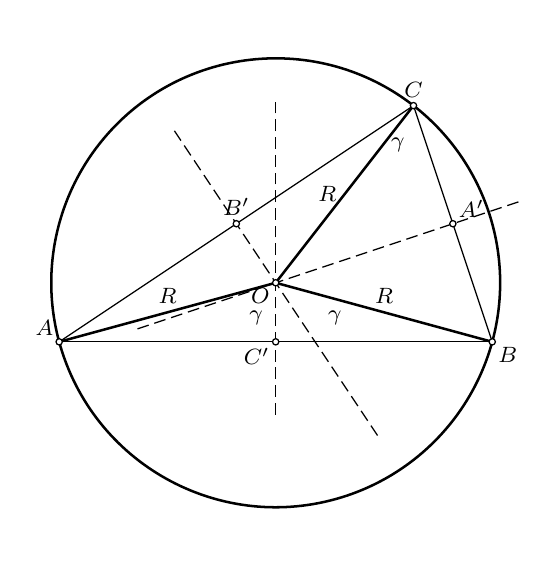
\begin{tikzpicture}
                % \clip (0,0) rectangle (14.000000,10.000000);
                {\footnotesize
                
                % Drawing segment A B
                \draw [line width=0.016cm] (1.540000,3.500000) -- (4.210000,3.500000);%
                \draw [line width=0.016cm] (4.290000,3.500000) -- (6.960000,3.500000);%
                
                % Drawing segment A C
                \draw [line width=0.016cm] (1.533282,3.522188) -- (3.716718,4.977812);%
                \draw [line width=0.016cm] (3.783282,5.022188) -- (5.966718,6.477812);%
                
                % Drawing segment B C
                \draw [line width=0.016cm] (6.987351,3.537947) -- (6.512649,4.962053);%
                \draw [line width=0.016cm] (6.487351,5.037947) -- (6.012649,6.462053);%
                
                % Drawing line a
                \draw [line width=0.016cm] (2.494176,3.664725) -- (2.636479,3.712160);%
                \draw [line width=0.016cm] (2.707630,3.735877) -- (2.849932,3.783311);%
                \draw [line width=0.016cm] (2.921084,3.807028) -- (3.063386,3.854462);%
                \draw [line width=0.016cm] (3.134537,3.878179) -- (3.276840,3.925613);%
                \draw [line width=0.016cm] (3.347991,3.949330) -- (3.490294,3.996765);%
                \draw [line width=0.016cm] (3.561445,4.020482) -- (3.703747,4.067916);%
                \draw [line width=0.016cm] (3.774899,4.091633) -- (3.917201,4.139067);%
                \draw [line width=0.016cm] (3.988352,4.162784) -- (4.130655,4.210218);%
                \draw [line width=0.016cm] (4.201806,4.233935) -- (4.212053,4.237351);%
                \draw [line width=0.016cm] (4.287947,4.262649) -- (4.344109,4.281370);%
                \draw [line width=0.016cm] (4.415260,4.305087) -- (4.557562,4.352521);%
                \draw [line width=0.016cm] (4.628714,4.376238) -- (4.771016,4.423672);%
                \draw [line width=0.016cm] (4.842167,4.447389) -- (4.984470,4.494823);%
                \draw [line width=0.016cm] (5.055621,4.518540) -- (5.197924,4.565975);%
                \draw [line width=0.016cm] (5.269075,4.589692) -- (5.411377,4.637126);%
                \draw [line width=0.016cm] (5.482529,4.660843) -- (5.624831,4.708277);%
                \draw [line width=0.016cm] (5.695982,4.731994) -- (5.838285,4.779428);%
                \draw [line width=0.016cm] (5.909436,4.803145) -- (6.051739,4.850580);%
                \draw [line width=0.016cm] (6.122890,4.874297) -- (6.265192,4.921731);%
                \draw [line width=0.016cm] (6.336344,4.945448) -- (6.462053,4.987351);%
                \draw [line width=0.016cm] (6.549797,5.016599) -- (6.692100,5.064033);%
                \draw [line width=0.016cm] (6.763251,5.087750) -- (6.905554,5.135185);%
                \draw [line width=0.016cm] (6.976705,5.158902) -- (7.119007,5.206336);%
                \draw [line width=0.016cm] (7.190159,5.230053) -- (7.332461,5.277487);%
                
                % Drawing line b
                \draw [line width=0.016cm] (5.543014,2.310479) -- (5.459809,2.435287);%
                \draw [line width=0.016cm] (5.418206,2.497691) -- (5.335001,2.622498);%
                \draw [line width=0.016cm] (5.293399,2.684902) -- (5.210194,2.809709);%
                \draw [line width=0.016cm] (5.168591,2.872113) -- (5.085386,2.996921);%
                \draw [line width=0.016cm] (5.043784,3.059324) -- (4.960579,3.184132);%
                \draw [line width=0.016cm] (4.918976,3.246536) -- (4.835771,3.371343);%
                \draw [line width=0.016cm] (4.794169,3.433747) -- (4.710964,3.558555);%
                \draw [line width=0.016cm] (4.669361,3.620958) -- (4.586156,3.745766);%
                \draw [line width=0.016cm] (4.544554,3.808170) -- (4.461348,3.932977);%
                \draw [line width=0.016cm] (4.419746,3.995381) -- (4.336541,4.120189);%
                \draw [line width=0.016cm] (4.294938,4.182592) -- (4.272188,4.216718);%
                \draw [line width=0.016cm] (4.227812,4.283282) -- (4.211733,4.307400);%
                \draw [line width=0.016cm] (4.170131,4.369804) -- (4.086926,4.494611);%
                \draw [line width=0.016cm] (4.045323,4.557015) -- (3.962118,4.681823);%
                \draw [line width=0.016cm] (3.920516,4.744226) -- (3.837311,4.869034);%
                \draw [line width=0.016cm] (3.795708,4.931438) -- (3.772188,4.966718);%
                \draw [line width=0.016cm] (3.727812,5.033282) -- (3.712503,5.056245);%
                \draw [line width=0.016cm] (3.670901,5.118649) -- (3.587696,5.243457);%
                \draw [line width=0.016cm] (3.546093,5.305860) -- (3.462888,5.430668);%
                \draw [line width=0.016cm] (3.421286,5.493072) -- (3.338081,5.617879);%
                \draw [line width=0.016cm] (3.296478,5.680283) -- (3.213273,5.805090);%
                \draw [line width=0.016cm] (3.171671,5.867494) -- (3.088465,5.992302);%
                \draw [line width=0.016cm] (3.046863,6.054706) -- (2.963658,6.179513);%
                
                % Drawing line c
                \draw [line width=0.016cm] (4.250000,2.575000) -- (4.250000,2.725000);%
                \draw [line width=0.016cm] (4.250000,2.800000) -- (4.250000,2.950000);%
                \draw [line width=0.016cm] (4.250000,3.025000) -- (4.250000,3.175000);%
                \draw [line width=0.016cm] (4.250000,3.250000) -- (4.250000,3.400000);%
                \draw [line width=0.016cm] (4.250000,3.540000) -- (4.250000,3.625000);%
                \draw [line width=0.016cm] (4.250000,3.700000) -- (4.250000,3.850000);%
                \draw [line width=0.016cm] (4.250000,3.925000) -- (4.250000,4.075000);%
                \draw [line width=0.016cm] (4.250000,4.150000) -- (4.250000,4.210000);%
                \draw [line width=0.016cm] (4.250000,4.290000) -- (4.250000,4.300000);%
                \draw [line width=0.016cm] (4.250000,4.375000) -- (4.250000,4.525000);%
                \draw [line width=0.016cm] (4.250000,4.600000) -- (4.250000,4.750000);%
                \draw [line width=0.016cm] (4.250000,4.825000) -- (4.250000,4.975000);%
                \draw [line width=0.016cm] (4.250000,5.050000) -- (4.250000,5.200000);%
                \draw [line width=0.016cm] (4.250000,5.275000) -- (4.250000,5.425000);%
                \draw [line width=0.016cm] (4.250000,5.500000) -- (4.250000,5.650000);%
                \draw [line width=0.016cm] (4.250000,5.725000) -- (4.250000,5.875000);%
                \draw [line width=0.016cm] (4.250000,5.950000) -- (4.250000,6.100000);%
                \draw [line width=0.016cm] (4.250000,6.175000) -- (4.250000,6.325000);%
                \draw [line width=0.016cm] (4.250000,6.400000) -- (4.250000,6.550000);%
                
                % Marking point A by circle
                \draw [line width=0.016cm] (1.500000,3.500000) circle (0.040000);%
                \draw (1.530000,3.470000) node [anchor=south east] { $A$ };%
                
                % Marking point B by circle
                \draw [line width=0.016cm] (7.000000,3.500000) circle (0.040000);%
                \draw (6.970000,3.530000) node [anchor=north west] { $B$ };%
                
                % Marking point C by circle
                \draw [line width=0.016cm] (6.000000,6.500000) circle (0.040000);%
                \draw (6.000000,6.500000) node [anchor=south] { $C$ };%
                
                % Marking point O by circle
                \draw [line width=0.016cm] (4.250000,4.250000) circle (0.040000);%
                \draw (4.280000,4.280000) node [anchor=north east] { $O$ };%
                
                % Marking point A' by circle
                \draw [line width=0.016cm] (6.500000,5.000000) circle (0.040000);%
                \draw (6.470000,4.970000) node [anchor=south west] { $A'$ };%
                
                % Marking point B' by circle
                \draw [line width=0.016cm] (3.750000,5.000000) circle (0.040000);%
                \draw (3.750000,5.000000) node [anchor=south] { $B'$ };%
                
                % Marking point C' by circle
                \draw [line width=0.016cm] (4.250000,3.500000) circle (0.040000);%
                \draw (4.280000,3.530000) node [anchor=north east] { $C'$ };%
                
                % Marking point \gamma
                \draw (4.000000,4.000000) node [anchor=north] { $\gamma$ };%
                
                % Marking point \gamma
                \draw (5.000000,4.000000) node [anchor=north] { $\gamma$ };%
                
                % Marking point \gamma
                \draw (5.800000,6.200000) node [anchor=north] { $\gamma$ };%
                
                % Marking point R
                \draw (2.875000,3.875000) node [anchor=south] { $R$ };%
                
                % Marking point R
                \draw (5.625000,3.875000) node [anchor=south] { $R$ };%
                
                % Marking point R
                \draw (5.125000,5.375000) node [anchor=east] { $R$ };%
                
                % Drawing segment A O
                \draw [line width=0.032cm] (1.538591,3.510525) -- (4.211409,4.239475);%
                
                % Drawing segment O B
                \draw [line width=0.032cm] (4.288591,4.239475) -- (6.961409,3.510525);%
                
                % Drawing segment O C
                \draw [line width=0.032cm] (4.274558,4.281574) -- (5.975442,6.468426);%
                
                % Drawing circle O A
                \draw [line width=0.032cm] (1.510795,3.461485) -- (1.524112,3.416613) arc (197:343:2.850439 and 2.850439) -- (6.989205,3.461483);%
                \draw [line width=0.032cm] (7.010253,3.538663) -- (7.015768,3.560416) arc (346:360:2.850439 and 2.850439) --(7.100439,4.250000) arc (0:51:2.850439 and 2.850439) -- (6.031401,6.475221);%
                \draw [line width=0.032cm] (5.968254,6.524335) -- (5.965437,6.526461) arc (53:194:2.850439 and 2.850439) -- (1.489746,3.538664);%
                }
            \end{tikzpicture}
            
        Z $R$ označimo polmer trikotniku očrtane krožnice. Ker je $\gamma$ obodni kot nad lokom $\arc{AB}$, je ustrezni središčni kot enak $2\gamma$. Zaradi skladnosti trikotnikov $\triangle AC'O\cong\triangle BC'O$ je $|\angle AOC|=\gamma$. Iz tega sledi $\sin\gamma=\frac{c}{2R}$. Iz formule za ploščino $p=\frac{a\cdot v_a}{2}=\frac{a\cdot b\cdot \sin\gamma}{2}$ dobimo $p=\frac{abc}{4R}$.

        Iz $4Rp=abc=s(s-b)(s-c)+s(s-a)(s-c)+s(s-a)(s-b)-(s-a)(s-b)(s-c)=\frac{p^2}{s-a}+\frac{p^2}{s-b}+\frac{p^2}{s-c}-\frac{p^2}{s}$ dobimo formulo za polmer očrtane krožnice: $4R=r_a+r_b+r_c-r$.

    \subsection*{Eulerjeva premica in višinska točka}

        Poznamo že nekaj posebnih točk v trikotniku: \begin{itemize}
            \item težišče $T$,
            \item središče včrtane krožnice $I$,
            \item središče očrtane krožnice $O$.
        \end{itemize}

        \noindent Če velja $T=O$, so težiščnice enake simetralam stranic in hkrati simetralam kotov. Iz tega sledi, da je tak trikotnik enakostraničen.

        \noindent Torej, če trikotnik $\triangle ABC$ ni enakostraničen, sta točki $T$ in $O$ različni, torej določata neko premico, ki jo imenujemo \textbf{Eulerjeva premica} trikotnika $\triangle ABC$.

            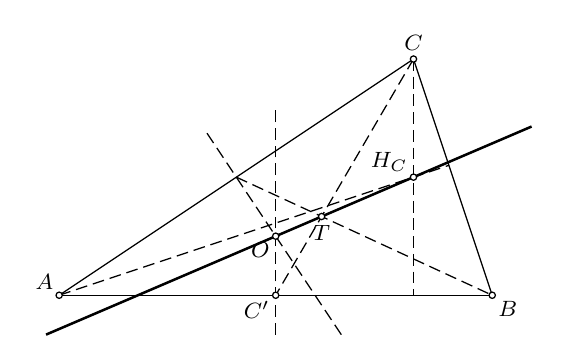
\begin{tikzpicture}
                % \clip (0,0) rectangle (14.000000,10.000000);
                {\footnotesize
                
                % Drawing segment A B
                \draw [line width=0.016cm] (1.540000,3.500000) -- (4.210000,3.500000);%
                \draw [line width=0.016cm] (4.290000,3.500000) -- (6.960000,3.500000);%
                
                % Drawing segment A C
                \draw [line width=0.016cm] (1.533282,3.522188) -- (5.966718,6.477812);%
                
                % Drawing segment B C
                \draw [line width=0.016cm] (6.987351,3.537947) -- (6.012649,6.462053);%
                
                % Drawing line b
                \draw [line width=0.016cm] (5.083333,3.000000) -- (5.000128,3.124808);%
                \draw [line width=0.016cm] (4.958526,3.187211) -- (4.875321,3.312019);%
                \draw [line width=0.016cm] (4.833718,3.374423) -- (4.750513,3.499230);%
                \draw [line width=0.016cm] (4.708911,3.561634) -- (4.625706,3.686441);%
                \draw [line width=0.016cm] (4.584103,3.748845) -- (4.500898,3.873653);%
                \draw [line width=0.016cm] (4.459296,3.936057) -- (4.376091,4.060864);%
                \draw [line width=0.016cm] (4.334488,4.123268) -- (4.272188,4.216718);%
                \draw [line width=0.016cm] (4.209681,4.310479) -- (4.126475,4.435287);%
                \draw [line width=0.016cm] (4.084873,4.497691) -- (4.001668,4.622498);%
                \draw [line width=0.016cm] (3.960065,4.684902) -- (3.876860,4.809709);%
                \draw [line width=0.016cm] (3.835258,4.872113) -- (3.752053,4.996921);%
                \draw [line width=0.016cm] (3.710450,5.059324) -- (3.627245,5.184132);%
                \draw [line width=0.016cm] (3.585643,5.246536) -- (3.502438,5.371343);%
                \draw [line width=0.016cm] (3.460835,5.433747) -- (3.377630,5.558555);%
                
                % Drawing line c
                \draw [line width=0.016cm] (4.250000,3.000000) -- (4.250000,3.150000);%
                \draw [line width=0.016cm] (4.250000,3.225000) -- (4.250000,3.375000);%
                \draw [line width=0.016cm] (4.250000,3.450000) -- (4.250000,3.460000);%
                \draw [line width=0.016cm] (4.250000,3.540000) -- (4.250000,3.600000);%
                \draw [line width=0.016cm] (4.250000,3.675000) -- (4.250000,3.825000);%
                \draw [line width=0.016cm] (4.250000,3.900000) -- (4.250000,4.050000);%
                \draw [line width=0.016cm] (4.250000,4.125000) -- (4.250000,4.210000);%
                \draw [line width=0.016cm] (4.250000,4.350000) -- (4.250000,4.500000);%
                \draw [line width=0.016cm] (4.250000,4.575000) -- (4.250000,4.725000);%
                \draw [line width=0.016cm] (4.250000,4.800000) -- (4.250000,4.950000);%
                \draw [line width=0.016cm] (4.250000,5.025000) -- (4.250000,5.175000);%
                \draw [line width=0.016cm] (4.250000,5.250000) -- (4.250000,5.400000);%
                \draw [line width=0.016cm] (4.250000,5.475000) -- (4.250000,5.625000);%
                \draw [line width=0.016cm] (4.250000,5.700000) -- (4.250000,5.850000);%
                
                % Drawing segment C C'
                \draw [line width=0.016cm] (5.979845,6.465449) -- (5.924419,6.370433);%
                \draw [line width=0.016cm] (5.886629,6.305650) -- (5.811048,6.176083);%
                \draw [line width=0.016cm] (5.773258,6.111299) -- (5.697677,5.981733);%
                \draw [line width=0.016cm] (5.659887,5.916949) -- (5.584306,5.787382);%
                \draw [line width=0.016cm] (5.546516,5.722599) -- (5.470935,5.593032);%
                \draw [line width=0.016cm] (5.433145,5.528249) -- (5.357564,5.398682);%
                \draw [line width=0.016cm] (5.319774,5.333898) -- (5.244193,5.204332);%
                \draw [line width=0.016cm] (5.206403,5.139548) -- (5.130822,5.009981);%
                \draw [line width=0.016cm] (5.093032,4.945198) -- (5.017452,4.815631);%
                \draw [line width=0.016cm] (4.979661,4.750848) -- (4.904081,4.621281);%
                \draw [line width=0.016cm] (4.866290,4.556497) -- (4.853488,4.534551);%
                \draw [line width=0.016cm] (4.813178,4.465449) -- (4.790710,4.426931);%
                \draw [line width=0.016cm] (4.752919,4.362147) -- (4.677339,4.232580);%
                \draw [line width=0.016cm] (4.639548,4.167797) -- (4.563968,4.038230);%
                \draw [line width=0.016cm] (4.526177,3.973447) -- (4.450597,3.843880);%
                \draw [line width=0.016cm] (4.412806,3.779096) -- (4.337226,3.649530);%
                \draw [line width=0.016cm] (4.299435,3.584746) -- (4.270155,3.534551);%
                
                % Drawing segment C U
                \draw [line width=0.016cm] (6.000000,6.460000) -- (6.000000,6.350000);%
                \draw [line width=0.016cm] (6.000000,6.275000) -- (6.000000,6.125000);%
                \draw [line width=0.016cm] (6.000000,6.050000) -- (6.000000,5.900000);%
                \draw [line width=0.016cm] (6.000000,5.825000) -- (6.000000,5.675000);%
                \draw [line width=0.016cm] (6.000000,5.600000) -- (6.000000,5.450000);%
                \draw [line width=0.016cm] (6.000000,5.375000) -- (6.000000,5.225000);%
                \draw [line width=0.016cm] (6.000000,5.150000) -- (6.000000,5.040000);%
                \draw [line width=0.016cm] (6.000000,4.925000) -- (6.000000,4.775000);%
                \draw [line width=0.016cm] (6.000000,4.700000) -- (6.000000,4.550000);%
                \draw [line width=0.016cm] (6.000000,4.475000) -- (6.000000,4.325000);%
                \draw [line width=0.016cm] (6.000000,4.250000) -- (6.000000,4.100000);%
                \draw [line width=0.016cm] (6.000000,4.025000) -- (6.000000,3.875000);%
                \draw [line width=0.016cm] (6.000000,3.800000) -- (6.000000,3.650000);%
                \draw [line width=0.016cm] (6.000000,3.575000) -- (6.000000,3.500000);%
                
                % Drawing segment A V
                \draw [line width=0.016cm] (1.537947,3.512649) -- (1.642302,3.547434);%
                \draw [line width=0.016cm] (1.713454,3.571151) -- (1.855756,3.618585);%
                \draw [line width=0.016cm] (1.926907,3.642302) -- (2.069210,3.689737);%
                \draw [line width=0.016cm] (2.140361,3.713454) -- (2.282664,3.760888);%
                \draw [line width=0.016cm] (2.353815,3.784605) -- (2.496117,3.832039);%
                \draw [line width=0.016cm] (2.567269,3.855756) -- (2.709571,3.903190);%
                \draw [line width=0.016cm] (2.780722,3.926907) -- (2.923025,3.974342);%
                \draw [line width=0.016cm] (2.994176,3.998059) -- (3.136479,4.045493);%
                \draw [line width=0.016cm] (3.207630,4.069210) -- (3.349932,4.116644);%
                \draw [line width=0.016cm] (3.421084,4.140361) -- (3.563386,4.187795);%
                \draw [line width=0.016cm] (3.634537,4.211512) -- (3.776840,4.258947);%
                \draw [line width=0.016cm] (3.847991,4.282664) -- (3.990294,4.330098);%
                \draw [line width=0.016cm] (4.061445,4.353815) -- (4.203747,4.401249);%
                \draw [line width=0.016cm] (4.274899,4.424966) -- (4.417201,4.472400);%
                \draw [line width=0.016cm] (4.488352,4.496117) -- (4.630655,4.543552);%
                \draw [line width=0.016cm] (4.701806,4.567269) -- (4.844109,4.614703);%
                \draw [line width=0.016cm] (4.915260,4.638420) -- (5.057562,4.685854);%
                \draw [line width=0.016cm] (5.128714,4.709571) -- (5.271016,4.757005);%
                \draw [line width=0.016cm] (5.342167,4.780722) -- (5.484470,4.828157);%
                \draw [line width=0.016cm] (5.555621,4.851874) -- (5.697924,4.899308);%
                \draw [line width=0.016cm] (5.769075,4.923025) -- (5.911377,4.970459);%
                \draw [line width=0.016cm] (6.037947,5.012649) -- (6.124831,5.041610);%
                \draw [line width=0.016cm] (6.195982,5.065327) -- (6.338285,5.112762);%
                \draw [line width=0.016cm] (6.409436,5.136479) -- (6.450000,5.150000);%
                
                % Drawing segment B' B
                \draw [line width=0.016cm] (3.750000,5.000000) -- (3.886194,4.937141);%
                \draw [line width=0.016cm] (3.954291,4.905712) -- (4.090485,4.842853);%
                \draw [line width=0.016cm] (4.158582,4.811424) -- (4.294776,4.748565);%
                \draw [line width=0.016cm] (4.362873,4.717136) -- (4.499066,4.654277);%
                \draw [line width=0.016cm] (4.567163,4.622848) -- (4.703357,4.559989);%
                \draw [line width=0.016cm] (4.771454,4.528560) -- (4.797015,4.516762);%
                \draw [line width=0.016cm] (4.869652,4.483238) -- (4.907648,4.465701);%
                \draw [line width=0.016cm] (4.975745,4.434271) -- (5.111939,4.371413);%
                \draw [line width=0.016cm] (5.180036,4.339983) -- (5.316230,4.277125);%
                \draw [line width=0.016cm] (5.384327,4.245695) -- (5.520521,4.182837);%
                \draw [line width=0.016cm] (5.588618,4.151407) -- (5.724812,4.088548);%
                \draw [line width=0.016cm] (5.792909,4.057119) -- (5.929103,3.994260);%
                \draw [line width=0.016cm] (5.997199,3.962831) -- (6.133393,3.899972);%
                \draw [line width=0.016cm] (6.201490,3.868543) -- (6.337684,3.805684);%
                \draw [line width=0.016cm] (6.405781,3.774255) -- (6.541975,3.711396);%
                \draw [line width=0.016cm] (6.610072,3.679967) -- (6.746266,3.617108);%
                \draw [line width=0.016cm] (6.814363,3.585679) -- (6.950557,3.522820);%
                
                % Marking point A by circle
                \draw [line width=0.016cm] (1.500000,3.500000) circle (0.040000);%
                \draw (1.530000,3.470000) node [anchor=south east] { $A$ };%
                
                % Marking point B by circle
                \draw [line width=0.016cm] (7.000000,3.500000) circle (0.040000);%
                \draw (6.970000,3.530000) node [anchor=north west] { $B$ };%
                
                % Marking point C by circle
                \draw [line width=0.016cm] (6.000000,6.500000) circle (0.040000);%
                \draw (6.000000,6.500000) node [anchor=south] { $C$ };%
                
                % Marking point O by circle
                \draw [line width=0.016cm] (4.250000,4.250000) circle (0.040000);%
                \draw (4.280000,4.280000) node [anchor=north east] { $O$ };%
                
                % Marking point C' by circle
                \draw [line width=0.016cm] (4.250000,3.500000) circle (0.040000);%
                \draw (4.280000,3.530000) node [anchor=north east] { $C'$ };%
                
                % Marking point T by circle
                \draw [line width=0.016cm] (4.833333,4.500000) circle (0.040000);%
                \draw (4.833333,4.500000) node [anchor=north] { $T$ };%
                
                % Marking point H_C by circle
                \draw [line width=0.016cm] (6.000000,5.000000) circle (0.040000);%
                \draw (6.030000,4.970000) node [anchor=south east] { $H_C$ };%
                
                % Drawing line O T
                \draw [line width=0.032cm] (1.333333,3.000000) -- (4.213234,4.234243);%
                \draw [line width=0.032cm] (4.286766,4.265757) -- (4.796568,4.484243);%
                \draw [line width=0.032cm] (4.870099,4.515757) -- (5.963234,4.984243);%
                \draw [line width=0.032cm] (6.036766,5.015757) -- (7.500000,5.642857);%
                }
            \end{tikzpicture}
            
        Naj bo $H_C$ presečišče (nosilke) višine iz $C$ in Eulerjeve premice. Velja $\overleftrightarrow{OC'}\parallel\overleftrightarrow{CH_C}$, saj sta obe premici pravokotni na premico $\overleftrightarrow{AB}$. Torej ti dve premici s poljubno prečnico oklepata skladna izmenična kota. Potem veljajo naslednje relacije: $\angle OC'T\cong\angle H_C CT$, $\angle C'OT\cong\angle CH_C T$, $\angle OTC'\cong\angle H_C TC$ (sovršnost). Iz tega sledi podobnost trikotnikov $\triangle OC'T\sim\triangle H_C CT$.
        Ker $T$ deli $C'C$ v razmerju $1:2$, sledi $\frac{|OT|}{|H_C T|}=\frac{|C'T|}{|TC|}=\frac{1}{2}$, iz tega pa sledi $|H_C T|=2|OT|$ in $O\ast T\ast H_C$.
        Ker analogno velja tudi glede na oglišči $A$ in $B$, sledi, da so $H_C=H_B=H_A=:H$, kar je \textbf{višinska točka}, ki je presečišče vseh treh višin trikotnika.

        Eulerjeva premica vsebuje točke $O$, $T$ in $H$ tako, da velja: \begin{itemize}
            \item $|TH|=2|OT|$ in
            \item $O\ast T\ast H$.
        \end{itemize}

    \subsection*{Krožnica devetih točk}

        \begin{definicija}
            V trikotniku $\triangle ABC$ zapovrstjo označimo nožišča višin iz $A,~B,~C$ s točkami $D,~E,~F$. Trikotnik $\triangle DEF$ immenujemo \textbf{višinski trikotnik} trikotnika $\triangle ABC$, njegovo očrtano krožnico pa \textbf{Feuerbachova krožnica} oziroma \textbf{krožnica devetih točk}.
        \end{definicija}

            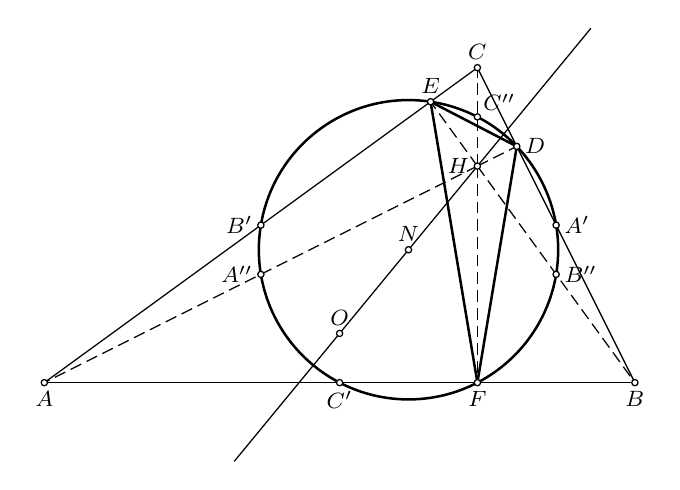
\begin{tikzpicture}
                % \clip (0,0) rectangle (14.000000,10.000000);
                {\footnotesize
                
                % Drawing segment A B
                \draw [line width=0.016cm] (1.540000,2.000000) -- (5.210000,2.000000);%
                \draw [line width=0.016cm] (5.290000,2.000000) -- (6.960000,2.000000);%
                \draw [line width=0.016cm] (7.040000,2.000000) -- (8.960000,2.000000);%
                
                % Drawing segment A C
                \draw [line width=0.016cm] (1.532349,2.023527) -- (4.217651,3.976473);%
                \draw [line width=0.016cm] (4.282349,4.023527) -- (6.373056,5.544041);%
                \draw [line width=0.016cm] (6.437755,5.591094) -- (6.967651,5.976473);%
                
                % Drawing segment B C
                \draw [line width=0.016cm] (8.982111,2.035777) -- (8.017889,3.964223);%
                \draw [line width=0.016cm] (7.982111,4.035777) -- (7.517889,4.964223);%
                \draw [line width=0.016cm] (7.482111,5.035777) -- (7.017889,5.964223);%
                
                % Marking point H by circle
                \draw [line width=0.016cm] (7.000000,4.750000) circle (0.040000);%
                \draw (7.000000,4.750000) node [anchor=east] { $H$ };%
                
                % Drawing line O T
                \draw [line width=0.016cm] (3.911765,1.000000) -- (5.224572,2.594123);%
                \draw [line width=0.016cm] (5.275428,2.655877) -- (6.099572,3.656623);%
                \draw [line width=0.016cm] (6.150428,3.718377) -- (6.974572,4.719123);%
                \draw [line width=0.016cm] (7.025428,4.780877) -- (8.441176,6.500000);%
                
                % Marking point A by circle
                \draw [line width=0.016cm] (1.500000,2.000000) circle (0.040000);%
                \draw (1.500000,2.000000) node [anchor=north] { $A$ };%
                
                % Marking point B by circle
                \draw [line width=0.016cm] (9.000000,2.000000) circle (0.040000);%
                \draw (9.000000,2.000000) node [anchor=north] { $B$ };%
                
                % Marking point C by circle
                \draw [line width=0.016cm] (7.000000,6.000000) circle (0.040000);%
                \draw (7.000000,6.000000) node [anchor=south] { $C$ };%
                
                % Marking point B' by circle
                \draw [line width=0.016cm] (4.250000,4.000000) circle (0.040000);%
                \draw (4.250000,4.000000) node [anchor=east] { $B'$ };%
                
                % Marking point A' by circle
                \draw [line width=0.016cm] (8.000000,4.000000) circle (0.040000);%
                \draw (8.000000,4.000000) node [anchor=west] { $A'$ };%
                
                % Marking point O by circle
                \draw [line width=0.016cm] (5.250000,2.625000) circle (0.040000);%
                \draw (5.250000,2.625000) node [anchor=south] { $O$ };%
                
                % Marking point E by circle
                \draw [line width=0.016cm] (6.405405,5.567568) circle (0.040000);%
                \draw (6.405405,5.567568) node [anchor=south] { $E$ };%
                
                % Marking point D by circle
                \draw [line width=0.016cm] (7.500000,5.000000) circle (0.040000);%
                \draw (7.500000,5.000000) node [anchor=west] { $D$ };%
                
                % Marking point F by circle
                \draw [line width=0.016cm] (7.000000,2.000000) circle (0.040000);%
                \draw (7.000000,2.000000) node [anchor=north] { $F$ };%
                
                % Drawing segment H B
                \draw [line width=0.016cm] (7.023527,4.717651) -- (7.088226,4.628690);%
                \draw [line width=0.016cm] (7.132339,4.568034) -- (7.220564,4.446724);%
                \draw [line width=0.016cm] (7.264677,4.386069) -- (7.352903,4.264758);%
                \draw [line width=0.016cm] (7.397016,4.204103) -- (7.485242,4.082793);%
                \draw [line width=0.016cm] (7.529355,4.022138) -- (7.617580,3.900827);%
                \draw [line width=0.016cm] (7.661693,3.840172) -- (7.749919,3.718861);%
                \draw [line width=0.016cm] (7.794032,3.658206) -- (7.882258,3.536896);%
                \draw [line width=0.016cm] (7.926370,3.476241) -- (7.976473,3.407349);%
                \draw [line width=0.016cm] (8.058709,3.294275) -- (8.146935,3.172965);%
                \draw [line width=0.016cm] (8.191048,3.112309) -- (8.279273,2.990999);%
                \draw [line width=0.016cm] (8.323386,2.930344) -- (8.411612,2.809033);%
                \draw [line width=0.016cm] (8.455725,2.748378) -- (8.543951,2.627068);%
                \draw [line width=0.016cm] (8.588064,2.566413) -- (8.676289,2.445102);%
                \draw [line width=0.016cm] (8.720402,2.384447) -- (8.808628,2.263137);%
                \draw [line width=0.016cm] (8.852741,2.202481) -- (8.940967,2.081171);%
                
                % Drawing segment H A
                \draw [line width=0.016cm] (6.964223,4.732111) -- (6.865836,4.682918);%
                \draw [line width=0.016cm] (6.798754,4.649377) -- (6.664590,4.582295);%
                \draw [line width=0.016cm] (6.597508,4.548754) -- (6.463344,4.481672);%
                \draw [line width=0.016cm] (6.396262,4.448131) -- (6.262098,4.381049);%
                \draw [line width=0.016cm] (6.195016,4.347508) -- (6.060851,4.280426);%
                \draw [line width=0.016cm] (5.993769,4.246885) -- (5.859605,4.179803);%
                \draw [line width=0.016cm] (5.792523,4.146262) -- (5.658359,4.079180);%
                \draw [line width=0.016cm] (5.591277,4.045639) -- (5.457113,3.978557);%
                \draw [line width=0.016cm] (5.390031,3.945016) -- (5.255867,3.877933);%
                \draw [line width=0.016cm] (5.188785,3.844392) -- (5.054621,3.777310);%
                \draw [line width=0.016cm] (4.987539,3.743769) -- (4.853375,3.676687);%
                \draw [line width=0.016cm] (4.786293,3.643146) -- (4.652129,3.576064);%
                \draw [line width=0.016cm] (4.585047,3.542523) -- (4.450883,3.475441);%
                \draw [line width=0.016cm] (4.383800,3.441900) -- (4.285777,3.392889);%
                \draw [line width=0.016cm] (4.182554,3.341277) -- (4.048390,3.274195);%
                \draw [line width=0.016cm] (3.981308,3.240654) -- (3.847144,3.173572);%
                \draw [line width=0.016cm] (3.780062,3.140031) -- (3.645898,3.072949);%
                \draw [line width=0.016cm] (3.578816,3.039408) -- (3.444652,2.972326);%
                \draw [line width=0.016cm] (3.377570,2.938785) -- (3.243406,2.871703);%
                \draw [line width=0.016cm] (3.176324,2.838162) -- (3.042160,2.771080);%
                \draw [line width=0.016cm] (2.975078,2.737539) -- (2.840914,2.670457);%
                \draw [line width=0.016cm] (2.773832,2.636916) -- (2.639667,2.569834);%
                \draw [line width=0.016cm] (2.572585,2.536293) -- (2.438421,2.469211);%
                \draw [line width=0.016cm] (2.371339,2.435670) -- (2.237175,2.368588);%
                \draw [line width=0.016cm] (2.170093,2.335047) -- (2.035929,2.267965);%
                \draw [line width=0.016cm] (1.968847,2.234424) -- (1.834683,2.167341);%
                \draw [line width=0.016cm] (1.767601,2.133800) -- (1.633437,2.066718);%
                \draw [line width=0.016cm] (1.566355,2.033177) -- (1.535777,2.017889);%
                
                % Drawing segment H C
                \draw [line width=0.016cm] (7.000000,4.790000) -- (7.000000,4.900000);%
                \draw [line width=0.016cm] (7.000000,4.975000) -- (7.000000,5.125000);%
                \draw [line width=0.016cm] (7.000000,5.200000) -- (7.000000,5.335000);%
                \draw [line width=0.016cm] (7.000000,5.425000) -- (7.000000,5.575000);%
                \draw [line width=0.016cm] (7.000000,5.650000) -- (7.000000,5.800000);%
                \draw [line width=0.016cm] (7.000000,5.875000) -- (7.000000,5.960000);%
                
                % Drawing segment H D
                \draw [line width=0.016cm] (7.035777,4.767889) -- (7.134164,4.817082);%
                \draw [line width=0.016cm] (7.201246,4.850623) -- (7.335410,4.917705);%
                \draw [line width=0.016cm] (7.402492,4.951246) -- (7.464223,4.982111);%
                
                % Drawing segment H E
                \draw [line width=0.016cm] (6.976473,4.782349) -- (6.911774,4.871310);%
                \draw [line width=0.016cm] (6.867661,4.931966) -- (6.779436,5.053276);%
                \draw [line width=0.016cm] (6.735323,5.113931) -- (6.647097,5.235242);%
                \draw [line width=0.016cm] (6.602984,5.295897) -- (6.514758,5.417207);%
                \draw [line width=0.016cm] (6.470645,5.477862) -- (6.428932,5.535218);%
                
                % Drawing segment H F
                \draw [line width=0.016cm] (7.000000,4.710000) -- (7.000000,4.600000);%
                \draw [line width=0.016cm] (7.000000,4.525000) -- (7.000000,4.375000);%
                \draw [line width=0.016cm] (7.000000,4.300000) -- (7.000000,4.150000);%
                \draw [line width=0.016cm] (7.000000,4.075000) -- (7.000000,3.925000);%
                \draw [line width=0.016cm] (7.000000,3.850000) -- (7.000000,3.700000);%
                \draw [line width=0.016cm] (7.000000,3.625000) -- (7.000000,3.475000);%
                \draw [line width=0.016cm] (7.000000,3.400000) -- (7.000000,3.250000);%
                \draw [line width=0.016cm] (7.000000,3.175000) -- (7.000000,3.025000);%
                \draw [line width=0.016cm] (7.000000,2.950000) -- (7.000000,2.800000);%
                \draw [line width=0.016cm] (7.000000,2.725000) -- (7.000000,2.575000);%
                \draw [line width=0.016cm] (7.000000,2.500000) -- (7.000000,2.350000);%
                \draw [line width=0.016cm] (7.000000,2.275000) -- (7.000000,2.125000);%
                \draw [line width=0.016cm] (7.000000,2.050000) -- (7.000000,2.040000);%
                
                % Marking point A'' by circle
                \draw [line width=0.016cm] (4.250000,3.375000) circle (0.040000);%
                \draw (4.250000,3.375000) node [anchor=east] { $A''$ };%
                
                % Marking point B'' by circle
                \draw [line width=0.016cm] (8.000000,3.375000) circle (0.040000);%
                \draw (8.000000,3.375000) node [anchor=west] { $B''$ };%
                
                % Marking point C'' by circle
                \draw [line width=0.016cm] (7.000000,5.375000) circle (0.040000);%
                \draw (6.970000,5.345000) node [anchor=south west] { $C''$ };%
                
                % Marking point C' by circle
                \draw [line width=0.016cm] (5.250000,2.000000) circle (0.040000);%
                \draw (5.250000,2.000000) node [anchor=north] { $C'$ };%
                
                % Marking point N by circle
                \draw [line width=0.016cm] (6.125000,3.687500) circle (0.040000);%
                \draw (6.125000,3.687500) node [anchor=south] { $N$ };%
                
                % Drawing circle N A'
                \draw [line width=0.032cm] (7.993009,4.039384) -- (7.990939,4.050202) arc (11:42:1.900863 and 1.900863) -- (7.527313,4.970777);%
                \draw [line width=0.032cm] (7.472078,5.028642) -- (7.469113,5.031613) arc (45:61:1.900863 and 1.900863) -- (7.035314,5.356215);%
                \draw [line width=0.032cm] (6.964298,5.393038) -- (6.958284,5.395985) arc (64:80:1.900863 and 1.900863) -- (6.444904,5.561251);%
                \draw [line width=0.032cm] (6.365783,5.573052) -- (6.356657,5.574195) arc (83:169:1.900863 and 1.900863) -- (4.256991,4.039384);%
                \draw [line width=0.032cm] (4.243840,3.960477) -- (4.242636,3.952049) arc (172:188:1.900863 and 1.900863) -- (4.243840,3.414523);%
                \draw [line width=0.032cm] (4.256991,3.335616) -- (4.259061,3.324798) arc (191:241:1.900863 and 1.900863) -- (5.214685,2.018786);%
                \draw [line width=0.032cm] (5.285701,1.981962) -- (5.291716,1.979016) arc (244:296:1.900863 and 1.900863) -- (6.964298,1.981962);%
                \draw [line width=0.032cm] (7.035314,2.018785) -- (7.046556,2.024967) arc (299:349:1.900863 and 1.900863) -- (7.993009,3.335615);%
                \draw [line width=0.032cm] (8.006160,3.414522) -- (8.007364,3.422950) arc (352:360:1.900863 and 1.900863) --(8.025863,3.687500) arc (0:8:1.900863 and 1.900863) -- (8.006161,3.960477);%
                
                % Drawing segment D E
                \draw [line width=0.032cm] (7.464490,5.018413) -- (6.440916,5.549155);%
                
                % Drawing segment D F
                \draw [line width=0.032cm] (7.493424,4.960544) -- (7.006576,2.039456);%
                
                % Drawing segment E F
                \draw [line width=0.032cm] (6.411981,5.528112) -- (6.993424,2.039456);%
                }
            \end{tikzpicture}

        \begin{izrek}
            Feuerbachova krožnica vsebuje nožišča višin, razpolovišča stranic in razpolovišča daljic od oglišč do višinske točke trikotnika.
        \end{izrek}

            \begin{dokaz}
                \\ 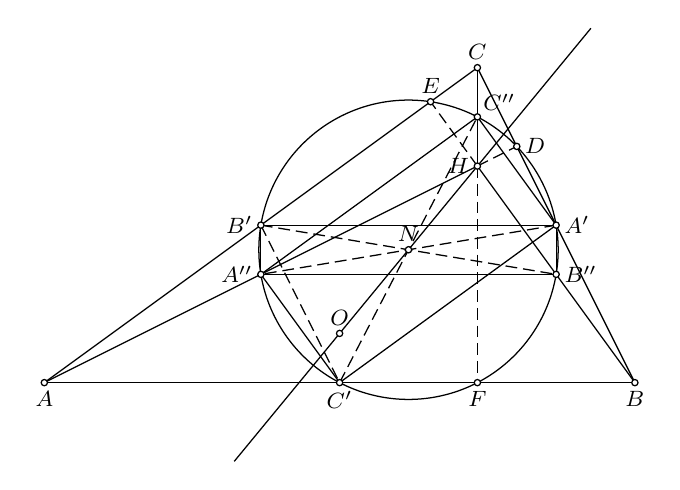
\begin{tikzpicture}
                    % \clip (0,0) rectangle (14.000000,10.000000);
                    {\footnotesize
                    
                    % Drawing segment A B
                    \draw [line width=0.016cm] (1.540000,2.000000) -- (5.210000,2.000000);%
                    \draw [line width=0.016cm] (5.290000,2.000000) -- (6.960000,2.000000);%
                    \draw [line width=0.016cm] (7.040000,2.000000) -- (8.960000,2.000000);%
                    
                    % Drawing segment A C
                    \draw [line width=0.016cm] (1.532349,2.023527) -- (4.217651,3.976473);%
                    \draw [line width=0.016cm] (4.282349,4.023527) -- (6.373056,5.544041);%
                    \draw [line width=0.016cm] (6.437755,5.591094) -- (6.967651,5.976473);%
                    
                    % Drawing segment B C
                    \draw [line width=0.016cm] (8.982111,2.035777) -- (8.017889,3.964223);%
                    \draw [line width=0.016cm] (7.982111,4.035777) -- (7.517889,4.964223);%
                    \draw [line width=0.016cm] (7.482111,5.035777) -- (7.017889,5.964223);%
                    
                    % Marking point H by circle
                    \draw [line width=0.016cm] (7.000000,4.750000) circle (0.040000);%
                    \draw (7.000000,4.750000) node [anchor=east] { $H$ };%
                    
                    % Drawing line O T
                    \draw [line width=0.016cm] (3.911765,1.000000) -- (5.224572,2.594123);%
                    \draw [line width=0.016cm] (5.275428,2.655877) -- (6.099572,3.656623);%
                    \draw [line width=0.016cm] (6.150428,3.718377) -- (6.974572,4.719123);%
                    \draw [line width=0.016cm] (7.025428,4.780877) -- (8.441176,6.500000);%
                    
                    % Marking point A by circle
                    \draw [line width=0.016cm] (1.500000,2.000000) circle (0.040000);%
                    \draw (1.500000,2.000000) node [anchor=north] { $A$ };%
                    
                    % Marking point B by circle
                    \draw [line width=0.016cm] (9.000000,2.000000) circle (0.040000);%
                    \draw (9.000000,2.000000) node [anchor=north] { $B$ };%
                    
                    % Marking point C by circle
                    \draw [line width=0.016cm] (7.000000,6.000000) circle (0.040000);%
                    \draw (7.000000,6.000000) node [anchor=south] { $C$ };%
                    
                    % Marking point B' by circle
                    \draw [line width=0.016cm] (4.250000,4.000000) circle (0.040000);%
                    \draw (4.250000,4.000000) node [anchor=east] { $B'$ };%
                    
                    % Marking point A' by circle
                    \draw [line width=0.016cm] (8.000000,4.000000) circle (0.040000);%
                    \draw (8.000000,4.000000) node [anchor=west] { $A'$ };%
                    
                    % Marking point O by circle
                    \draw [line width=0.016cm] (5.250000,2.625000) circle (0.040000);%
                    \draw (5.250000,2.625000) node [anchor=south] { $O$ };%
                    
                    % Marking point E by circle
                    \draw [line width=0.016cm] (6.405405,5.567568) circle (0.040000);%
                    \draw (6.405405,5.567568) node [anchor=south] { $E$ };%
                    
                    % Marking point D by circle
                    \draw [line width=0.016cm] (7.500000,5.000000) circle (0.040000);%
                    \draw (7.500000,5.000000) node [anchor=west] { $D$ };%
                    
                    % Marking point F by circle
                    \draw [line width=0.016cm] (7.000000,2.000000) circle (0.040000);%
                    \draw (7.000000,2.000000) node [anchor=north] { $F$ };%
                    
                    % Marking point N by circle
                    \draw [line width=0.016cm] (6.125000,3.687500) circle (0.040000);%
                    \draw (6.125000,3.687500) node [anchor=south] { $N$ };%
                    
                    % Drawing segment B' A'
                    \draw [line width=0.016cm] (4.290000,4.000000) -- (7.960000,4.000000);%
                    
                    % Drawing segment H B
                    \draw [line width=0.016cm] (7.023527,4.717651) -- (7.976473,3.407349);%
                    \draw [line width=0.016cm] (8.023527,3.342651) -- (8.976473,2.032349);%
                    
                    % Drawing segment H A
                    \draw [line width=0.016cm] (6.964223,4.732111) -- (4.285777,3.392889);%
                    \draw [line width=0.016cm] (4.214223,3.357111) -- (1.535777,2.017889);%
                    
                    % Drawing segment H C
                    \draw [line width=0.016cm] (7.000000,4.790000) -- (7.000000,5.335000);%
                    \draw [line width=0.016cm] (7.000000,5.415000) -- (7.000000,5.960000);%
                    
                    % Drawing segment H D
                    \draw [line width=0.016cm] (7.035777,4.767889) -- (7.134164,4.817082);%
                    \draw [line width=0.016cm] (7.201246,4.850623) -- (7.335410,4.917705);%
                    \draw [line width=0.016cm] (7.402492,4.951246) -- (7.464223,4.982111);%
                    
                    % Drawing segment H E
                    \draw [line width=0.016cm] (6.976473,4.782349) -- (6.911774,4.871310);%
                    \draw [line width=0.016cm] (6.867661,4.931966) -- (6.779436,5.053276);%
                    \draw [line width=0.016cm] (6.735323,5.113931) -- (6.647097,5.235242);%
                    \draw [line width=0.016cm] (6.602984,5.295897) -- (6.514758,5.417207);%
                    \draw [line width=0.016cm] (6.470645,5.477862) -- (6.428932,5.535218);%
                    
                    % Drawing segment H F
                    \draw [line width=0.016cm] (7.000000,4.710000) -- (7.000000,4.600000);%
                    \draw [line width=0.016cm] (7.000000,4.525000) -- (7.000000,4.375000);%
                    \draw [line width=0.016cm] (7.000000,4.300000) -- (7.000000,4.150000);%
                    \draw [line width=0.016cm] (7.000000,4.075000) -- (7.000000,3.925000);%
                    \draw [line width=0.016cm] (7.000000,3.850000) -- (7.000000,3.700000);%
                    \draw [line width=0.016cm] (7.000000,3.625000) -- (7.000000,3.475000);%
                    \draw [line width=0.016cm] (7.000000,3.400000) -- (7.000000,3.250000);%
                    \draw [line width=0.016cm] (7.000000,3.175000) -- (7.000000,3.025000);%
                    \draw [line width=0.016cm] (7.000000,2.950000) -- (7.000000,2.800000);%
                    \draw [line width=0.016cm] (7.000000,2.725000) -- (7.000000,2.575000);%
                    \draw [line width=0.016cm] (7.000000,2.500000) -- (7.000000,2.350000);%
                    \draw [line width=0.016cm] (7.000000,2.275000) -- (7.000000,2.125000);%
                    \draw [line width=0.016cm] (7.000000,2.050000) -- (7.000000,2.040000);%
                    
                    % Drawing segment B'' A''
                    \draw [line width=0.016cm] (7.960000,3.375000) -- (4.290000,3.375000);%
                    
                    % Marking point A'' by circle
                    \draw [line width=0.016cm] (4.250000,3.375000) circle (0.040000);%
                    \draw (4.250000,3.375000) node [anchor=east] { $A''$ };%
                    
                    % Marking point B'' by circle
                    \draw [line width=0.016cm] (8.000000,3.375000) circle (0.040000);%
                    \draw (8.000000,3.375000) node [anchor=west] { $B''$ };%
                    
                    % Drawing segment A' A''
                    \draw [line width=0.016cm] (7.960544,3.993424) -- (7.852041,3.975340);%
                    \draw [line width=0.016cm] (7.778061,3.963010) -- (7.630102,3.938350);%
                    \draw [line width=0.016cm] (7.556123,3.926020) -- (7.408164,3.901361);%
                    \draw [line width=0.016cm] (7.334184,3.889031) -- (7.186225,3.864371);%
                    \draw [line width=0.016cm] (7.112245,3.852041) -- (6.964286,3.827381);%
                    \draw [line width=0.016cm] (6.890307,3.815051) -- (6.742348,3.790391);%
                    \draw [line width=0.016cm] (6.668368,3.778061) -- (6.520409,3.753402);%
                    \draw [line width=0.016cm] (6.446430,3.741072) -- (6.298470,3.716412);%
                    \draw [line width=0.016cm] (6.224491,3.704082) -- (6.164456,3.694076);%
                    \draw [line width=0.016cm] (6.085544,3.680924) -- (6.076532,3.679422);%
                    \draw [line width=0.016cm] (6.002552,3.667092) -- (5.854593,3.642432);%
                    \draw [line width=0.016cm] (5.780614,3.630102) -- (5.632655,3.605442);%
                    \draw [line width=0.016cm] (5.558675,3.593113) -- (5.410716,3.568453);%
                    \draw [line width=0.016cm] (5.336736,3.556123) -- (5.188777,3.531463);%
                    \draw [line width=0.016cm] (5.114798,3.519133) -- (4.966839,3.494473);%
                    \draw [line width=0.016cm] (4.892859,3.482143) -- (4.744900,3.457483);%
                    \draw [line width=0.016cm] (4.670921,3.445153) -- (4.522961,3.420494);%
                    \draw [line width=0.016cm] (4.448982,3.408164) -- (4.301023,3.383504);%
                    
                    % Drawing segment B' B''
                    \draw [line width=0.016cm] (4.289456,3.993424) -- (4.397959,3.975340);%
                    \draw [line width=0.016cm] (4.471939,3.963010) -- (4.619898,3.938350);%
                    \draw [line width=0.016cm] (4.693877,3.926020) -- (4.841836,3.901361);%
                    \draw [line width=0.016cm] (4.915816,3.889031) -- (5.063775,3.864371);%
                    \draw [line width=0.016cm] (5.137755,3.852041) -- (5.285714,3.827381);%
                    \draw [line width=0.016cm] (5.359693,3.815051) -- (5.507652,3.790391);%
                    \draw [line width=0.016cm] (5.581632,3.778061) -- (5.729591,3.753402);%
                    \draw [line width=0.016cm] (5.803570,3.741072) -- (5.951530,3.716412);%
                    \draw [line width=0.016cm] (6.025509,3.704082) -- (6.085544,3.694076);%
                    \draw [line width=0.016cm] (6.164456,3.680924) -- (6.173468,3.679422);%
                    \draw [line width=0.016cm] (6.247448,3.667092) -- (6.395407,3.642432);%
                    \draw [line width=0.016cm] (6.469386,3.630102) -- (6.617345,3.605442);%
                    \draw [line width=0.016cm] (6.691325,3.593113) -- (6.839284,3.568453);%
                    \draw [line width=0.016cm] (6.913264,3.556123) -- (7.061223,3.531463);%
                    \draw [line width=0.016cm] (7.135202,3.519133) -- (7.283161,3.494473);%
                    \draw [line width=0.016cm] (7.357141,3.482143) -- (7.505100,3.457483);%
                    \draw [line width=0.016cm] (7.579079,3.445153) -- (7.727039,3.420494);%
                    \draw [line width=0.016cm] (7.801018,3.408164) -- (7.948977,3.383504);%
                    
                    % Drawing segment B' A''
                    \draw [line width=0.016cm] (4.250000,3.960000) -- (4.250000,3.415000);%
                    
                    % Drawing segment A' B''
                    \draw [line width=0.016cm] (8.000000,3.960000) -- (8.000000,3.415000);%
                    
                    % Marking point C'' by circle
                    \draw [line width=0.016cm] (7.000000,5.375000) circle (0.040000);%
                    \draw (6.970000,5.345000) node [anchor=south west] { $C''$ };%
                    
                    % Marking point C' by circle
                    \draw [line width=0.016cm] (5.250000,2.000000) circle (0.040000);%
                    \draw (5.250000,2.000000) node [anchor=north] { $C'$ };%
                    
                    % Drawing segment C' C''
                    \draw [line width=0.016cm] (5.268413,2.035510) -- (5.319048,2.133163);%
                    \draw [line width=0.016cm] (5.353571,2.199745) -- (5.422619,2.332908);%
                    \draw [line width=0.016cm] (5.457143,2.399490) -- (5.526190,2.532653);%
                    \draw [line width=0.016cm] (5.560714,2.599234) -- (5.629762,2.732397);%
                    \draw [line width=0.016cm] (5.664285,2.798979) -- (5.733333,2.932142);%
                    \draw [line width=0.016cm] (5.767857,2.998724) -- (5.836904,3.131887);%
                    \draw [line width=0.016cm] (5.871428,3.198469) -- (5.940476,3.331632);%
                    \draw [line width=0.016cm] (5.975000,3.398213) -- (6.044047,3.531377);%
                    \draw [line width=0.016cm] (6.078571,3.597958) -- (6.106587,3.651990);%
                    \draw [line width=0.016cm] (6.143413,3.723010) -- (6.147618,3.731121);%
                    \draw [line width=0.016cm] (6.182142,3.797703) -- (6.251190,3.930866);%
                    \draw [line width=0.016cm] (6.285714,3.997448) -- (6.354761,4.130611);%
                    \draw [line width=0.016cm] (6.389285,4.197192) -- (6.458333,4.330356);%
                    \draw [line width=0.016cm] (6.492856,4.396937) -- (6.561904,4.530100);%
                    \draw [line width=0.016cm] (6.596428,4.596682) -- (6.665475,4.729845);%
                    \draw [line width=0.016cm] (6.699999,4.796427) -- (6.769047,4.929590);%
                    \draw [line width=0.016cm] (6.803570,4.996172) -- (6.872618,5.129335);%
                    \draw [line width=0.016cm] (6.907142,5.195916) -- (6.976189,5.329079);%
                    
                    % Drawing segment A'' C'
                    \draw [line width=0.016cm] (4.273527,3.342651) -- (5.226473,2.032349);%
                    
                    % Drawing segment C' A'
                    \draw [line width=0.016cm] (5.282349,2.023527) -- (7.967651,3.976473);%
                    
                    % Drawing segment C'' A''
                    \draw [line width=0.016cm] (6.967651,5.351473) -- (4.282349,3.398527);%
                    
                    % Drawing segment A' C''
                    \draw [line width=0.016cm] (7.976473,4.032349) -- (7.023527,5.342651);%
                    
                    % Drawing segment B' C'
                    \draw [line width=0.016cm] (4.267889,3.964223) -- (4.317082,3.865836);%
                    \draw [line width=0.016cm] (4.350623,3.798754) -- (4.417705,3.664590);%
                    \draw [line width=0.016cm] (4.451246,3.597508) -- (4.518328,3.463344);%
                    \draw [line width=0.016cm] (4.551869,3.396262) -- (4.618951,3.262098);%
                    \draw [line width=0.016cm] (4.652492,3.195016) -- (4.719574,3.060851);%
                    \draw [line width=0.016cm] (4.753115,2.993769) -- (4.820197,2.859605);%
                    \draw [line width=0.016cm] (4.853738,2.792523) -- (4.920820,2.658359);%
                    \draw [line width=0.016cm] (4.954361,2.591277) -- (5.021443,2.457113);%
                    \draw [line width=0.016cm] (5.054984,2.390031) -- (5.122067,2.255867);%
                    \draw [line width=0.016cm] (5.155608,2.188785) -- (5.222690,2.054621);%
                    
                    % Drawing circle N A'
                    \draw [line width=0.016cm] (7.993009,4.039384) -- (7.990939,4.050202) arc (11:42:1.900863 and 1.900863) -- (7.527313,4.970777);%
                    \draw [line width=0.016cm] (7.472078,5.028642) -- (7.469113,5.031613) arc (45:61:1.900863 and 1.900863) -- (7.035314,5.356215);%
                    \draw [line width=0.016cm] (6.964298,5.393038) -- (6.958284,5.395985) arc (64:80:1.900863 and 1.900863) -- (6.444904,5.561251);%
                    \draw [line width=0.016cm] (6.365783,5.573052) -- (6.356657,5.574195) arc (83:169:1.900863 and 1.900863) -- (4.256991,4.039384);%
                    \draw [line width=0.016cm] (4.243840,3.960477) -- (4.242636,3.952049) arc (172:188:1.900863 and 1.900863) -- (4.243840,3.414523);%
                    \draw [line width=0.016cm] (4.256991,3.335616) -- (4.259061,3.324798) arc (191:241:1.900863 and 1.900863) -- (5.214685,2.018786);%
                    \draw [line width=0.016cm] (5.285701,1.981962) -- (5.291716,1.979016) arc (244:296:1.900863 and 1.900863) -- (6.964298,1.981962);%
                    \draw [line width=0.016cm] (7.035314,2.018785) -- (7.046556,2.024967) arc (299:349:1.900863 and 1.900863) -- (7.993009,3.335615);%
                    \draw [line width=0.016cm] (8.006160,3.414522) -- (8.007364,3.422950) arc (352:360:1.900863 and 1.900863) --(8.025863,3.687500) arc (0:8:1.900863 and 1.900863) -- (8.006161,3.960477);%
                    }
                    \end{tikzpicture}
                \\ Trikotnika $\triangle ABC$ in $\triangle B'A'C'$ sta podobna s faktorjem $\frac{1}{2}$ in zato sta premici $\overleftrightarrow{AB}$ in $\overleftrightarrow{B'A'}$ vzporedni: $\overleftrightarrow{AB}\parallel\overleftrightarrow{B'A'}$. Trikotnika $\triangle ABH$ in $\triangle A''B''H'$ sta podobna s faktorjem $\frac{1}{2}$ in zato sta premici $\overleftrightarrow{AB}$ in $\overleftrightarrow{B''A''}$ vzporedni: $\overleftrightarrow{AB}\parallel\overleftrightarrow{B''A''}$. Iz tega sledi: $\overleftrightarrow{A'B'}\parallel\overleftrightarrow{A''B''}$.
                Podobno veljata podobnosti trikotnikov $\triangle AHC\sim\triangle AA''B'$ in $\triangle BHC\sim\triangle BB''A'$, s faktorjem $\frac{1}{2}$, zato veljajo vzporednosti: $\overleftrightarrow{B'A''}\parallel\overleftrightarrow{CH}\parallel\overleftrightarrow{A'B''}$. Od tod sledi, da je štirikotnik $\square A'B'A''B''$ pralelogram, še več, to je pravokotnik, ker je $\overleftrightarrow{CH}\perp\overleftrightarrow{AB}$. Torej točke $A',~A'',~B',~B''$ ležijo na isti krožnici, katere središče je presečišče (razpolovišče) diagonal pravokotnika.
                Analogno/simetrično sledi, da so $A',~C',~A'',~C''$ tudi na eni krožnici, ki je očrtana pravokotniku $\square A'C'A''C''$, katere središče je razpolovišče diagonal. Ta dva pravokotnika imata skupno diagonalo $A'A''$, zato središči krožnic sovpadata, prav tako tudi polmera. 
                Torej je vseh šest točk $A',~B',~C',~A'',~B'',~C''$ na tej krožnici, v kateri so tetive $A'A''$, $B'B''$ in $C'C''$ premeri. Ker je kot $\angle B'EB''$ pravi kot, leži točka $E$ na krožnici s premerom $B'B''$ (Tales). Enak sklep velja za točki: $D$ glede na $A'A''$ in $F$ glede na $C'C''$.
            \end{dokaz}

        \begin{opomba}
            Feuerbachova krožnica je tudi očrtana krožnica za težiščni trikotnik.
        \end{opomba}

        \begin{posledica}
            Srediče $N$ Feuerbachove krožnice leži na Eulerjevi premici in razpolavlja daljico $OH$.
        \end{posledica}

            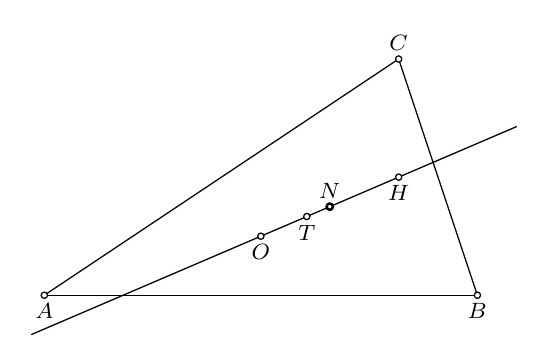
\begin{tikzpicture}
                % \clip (0,0) rectangle (14.000000,10.000000);
                {\footnotesize
                
                % Drawing segment A B
                \draw [line width=0.016cm] (1.540000,3.500000) -- (6.960000,3.500000);%
                
                % Drawing segment A C
                \draw [line width=0.016cm] (1.533282,3.522188) -- (5.966718,6.477812);%
                
                % Drawing segment B C
                \draw [line width=0.016cm] (6.987351,3.537947) -- (6.012649,6.462053);%
                
                % Marking point T by circle
                \draw [line width=0.016cm] (4.833333,4.500000) circle (0.040000);%
                \draw (4.833333,4.500000) node [anchor=north] { $T$ };%
                
                % Marking point H by circle
                \draw [line width=0.016cm] (6.000000,5.000000) circle (0.040000);%
                \draw (6.000000,5.000000) node [anchor=north] { $H$ };%
                
                % Drawing line O T
                \draw [line width=0.016cm] (1.333333,3.000000) -- (4.213234,4.234243);%
                \draw [line width=0.016cm] (4.286766,4.265757) -- (4.796568,4.484243);%
                \draw [line width=0.016cm] (4.870099,4.515757) -- (5.088234,4.609243);%
                \draw [line width=0.016cm] (5.161766,4.640757) -- (5.963234,4.984243);%
                \draw [line width=0.016cm] (6.036766,5.015757) -- (7.500000,5.642857);%
                
                % Marking point A by circle
                \draw [line width=0.016cm] (1.500000,3.500000) circle (0.040000);%
                \draw (1.500000,3.500000) node [anchor=north] { $A$ };%
                
                % Marking point B by circle
                \draw [line width=0.016cm] (7.000000,3.500000) circle (0.040000);%
                \draw (7.000000,3.500000) node [anchor=north] { $B$ };%
                
                % Marking point C by circle
                \draw [line width=0.016cm] (6.000000,6.500000) circle (0.040000);%
                \draw (6.000000,6.500000) node [anchor=south] { $C$ };%
                
                % Marking point O by circle
                \draw [line width=0.016cm] (4.250000,4.250000) circle (0.040000);%
                \draw (4.250000,4.250000) node [anchor=north] { $O$ };%
                
                % Marking point N by circle
                \draw [line width=0.032cm] (5.125000,4.625000) circle (0.040000);%
                \draw (5.125000,4.625000) node [anchor=south] { $N$ };%
                }
            \end{tikzpicture}  

            \begin{dokaz}     
                \\ Feuerbachova krožnica je očrtana krožnica težiščnega trikotnika $\triangle A'B'C'$, ki ga dobimo iz trikotnika $\triangle ABC$ z raztegom $R(T, -\frac{1}{2})$. Pri tem raztegu se torej očrtana krožnica trikotnika $\triangle ABC$, s središčem $O$, preslika v očrtano krožnico trikotnika $\triangle A'B'C'$, s središčem $N$. Torej je $N$ slika $O$ pri raztegu $R(T, -\frac{1}{2})$ in velja: $O\ast T\ast N$ in $ |TN|=\frac{1}{2}|OT|$. Velja: $|OT|=\frac{1}{3}|OH| \Rightarrow |TN|=\frac{1}{6}|OH|$ in $|ON|=|NT|+|TO|=(\frac{1}{3}+\frac{1}{6})|OH|=\frac{1}{2}|OH|$.
            \end{dokaz}

    \subsection*{Tetivni štirikotnik}

        \begin{definicija}
            Če točke $A,~B,~C,~D$ ležijo na isti krožnici v takem cikličnem vrstnem redu, pravimo, da je $\square ABCD$ \textbf{tetivni štirikotnik}.
        \end{definicija}

            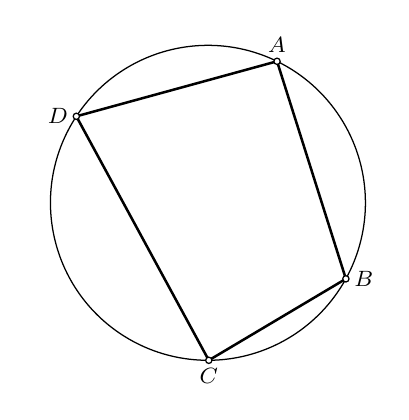
\begin{tikzpicture}
                % \clip (0,0) rectangle (14.000000,10.000000);
                {\footnotesize
                
                % Drawing circle K
                \draw [line width=0.016cm] (5.500000,3.500000) arc (0:62:2.000000 and 2.000000) -- (4.413198,5.279345);%
                \draw [line width=0.016cm] (4.341311,5.314441) -- (4.313473,5.327091) arc (66:145:2.000000 and 2.000000) -- (1.850962,4.631669);%
                \draw [line width=0.016cm] (1.807026,4.564819) -- (1.803904,4.559839) arc (148:269:2.000000 and 2.000000) -- (3.470738,1.500214);%
                \draw [line width=0.016cm] (3.550733,1.500644) -- (3.569799,1.501218) arc (272:329:2.000000 and 2.000000) -- (5.231961,2.499844);%
                \draw [line width=0.016cm] (5.270571,2.569905) -- (5.282013,2.592018) arc (333:360:2.000000 and 2.000000) --(5.500000,3.500000) arc (0:0:2.000000 and 2.000000);%
                
                % Marking point A by circle
                \draw [line width=0.016cm] (4.377430,5.297253) circle (0.040000);%
                \draw (4.377430,5.297253) node [anchor=south] { $A$ };%
                
                % Marking point B by circle
                \draw [line width=0.016cm] (5.251617,2.534682) circle (0.040000);%
                \draw (5.251617,2.534682) node [anchor=west] { $B$ };%
                
                % Marking point C by circle
                \draw [line width=0.016cm] (3.510738,1.500029) circle (0.040000);%
                \draw (3.510738,1.500029) node [anchor=north] { $C$ };%
                
                % Marking point D by circle
                \draw [line width=0.016cm] (1.828660,4.598463) circle (0.040000);%
                \draw (1.828660,4.598463) node [anchor=east] { $D$ };%
                
                % Drawing segment A B
                \draw [line width=0.032cm] (4.389498,5.259116) -- (5.239549,2.572818);%
                
                % Drawing segment B C
                \draw [line width=0.032cm] (5.217231,2.514245) -- (3.545124,1.520465);%
                
                % Drawing segment C D
                \draw [line width=0.032cm] (3.491654,1.535183) -- (1.847744,4.563310);%
                
                % Drawing segment D A
                \draw [line width=0.032cm] (1.867236,4.609040) -- (4.338854,5.286676);%
                }
            \end{tikzpicture}            

        \begin{trditev}
            Naj bodo točke $A,~B,~C,~D$ take različne točke, da točki $C,~D$ ležita na istem bregu  premice $\overleftrightarrow{AB}$. $\square ABCD$ je tetivni štirikotnik natanko tedaj, ko velja skladnost kotov: $\angle ACB\cong\angle ADB$.
        \end{trditev}

            \begin{dokaz}
                \\ ($\Rightarrow$): sledi iz izreka o središčnem in obodnem kotu
                \\ ($\Leftarrow$): 
                \\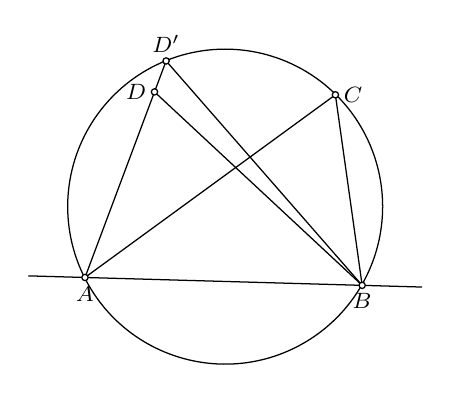
\begin{tikzpicture}
                    % \clip (0,0) rectangle (14.000000,10.000000);
                    {\footnotesize
                    
                    % Drawing circle K
                    \draw [line width=0.016cm] (5.500000,3.500000) arc (0:44:2.000000 and 2.000000) -- (4.932085,4.896114);%
                    \draw [line width=0.016cm] (4.875661,4.951743) -- (4.863997,4.962707) arc (47:110:2.000000 and 2.000000) -- (2.785678,5.368086);%
                    \draw [line width=0.016cm] (2.711800,5.338135) -- (2.686527,5.327091) arc (114:205:2.000000 and 2.000000) -- (1.697619,2.633153);%
                    \draw [line width=0.016cm] (1.733432,2.562323) -- (1.734105,2.561057) arc (208:328:2.000000 and 2.000000) -- (5.214093,2.469522);%
                    \draw [line width=0.016cm] (5.253291,2.537727) -- (5.265895,2.561056) arc (332:360:2.000000 and 2.000000) --(5.500000,3.500000) arc (0:0:2.000000 and 2.000000);%
                    
                    % Marking point A by circle
                    \draw [line width=0.016cm] (1.720000,2.600000) circle (0.040000);%
                    \draw (1.720000,2.600000) node [anchor=north] { $A$ };%
                    
                    % Marking point B by circle
                    \draw [line width=0.016cm] (5.240000,2.500000) circle (0.040000);%
                    \draw (5.240000,2.500000) node [anchor=north] { $B$ };%
                    
                    % Marking point C by circle
                    \draw [line width=0.016cm] (4.900000,4.920000) circle (0.040000);%
                    \draw (4.900000,4.920000) node [anchor=west] { $C$ };%
                    
                    % Marking point D' by circle
                    \draw [line width=0.016cm] (2.750000,5.350000) circle (0.040000);%
                    \draw (2.750000,5.350000) node [anchor=south] { $D'$ };%
                    
                    % Drawing line A B
                    \draw [line width=0.016cm] (1.000000,2.620455) -- (1.680016,2.601136);%
                    \draw [line width=0.016cm] (1.759984,2.598864) -- (5.200016,2.501136);%
                    \draw [line width=0.016cm] (5.279984,2.498864) -- (6.000000,2.478409);%
                    
                    % Drawing segment B C
                    \draw [line width=0.016cm] (5.234435,2.539611) -- (4.905565,4.880389);%
                    
                    % Drawing segment B D'
                    \draw [line width=0.016cm] (5.213682,2.530123) -- (2.776318,5.319877);%
                    
                    % Drawing segment D' A
                    \draw [line width=0.016cm] (2.735970,5.312541) -- (2.616761,4.994266);%
                    \draw [line width=0.016cm] (2.588701,4.919348) -- (1.734030,2.637459);%
                    
                    % Drawing segment A C
                    \draw [line width=0.016cm] (1.752314,2.623575) -- (4.867686,4.896425);%
                    
                    % Marking point D by circle
                    \draw [line width=0.016cm] (2.602731,4.956807) circle (0.040000);%
                    \draw (2.602731,4.956807) node [anchor=east] { $D$ };%
                    
                    % Drawing segment B D
                    \draw [line width=0.016cm] (5.210732,2.527265) -- (2.631999,4.929542);%
                    }
                    \end{tikzpicture}                    
                \\ Naj bo $K$ trikotniku $\triangle ABC$ očrtana krožnica. Denimo, da $D$ leži znotraj krožnice $K$. Naj bo točka $D'$ presečišče poltraka $\overrightarrow{AD}$ in krožnie $K$. Potem je $\angle AD'B\cong\angle ACB$ po izreku o obodnih kotih. To nas privede v protislovje (zunanji kot trikotnika $\triangle BDD'$ je skladen z notranjim kotom pri $D'$.)
            \end{dokaz}
        
        \begin{posledica}
            $\square ABCD$ je tetivni štirikotnik natanko tedaj, ko je vsota kotov ob nasprotnih ogliščih enaka $\pi$.
        \end{posledica}

            \begin{dokaz}
                \\ \begin{tikzpicture}
                    % \clip (0,0) rectangle (14.000000,10.000000);
                    {\footnotesize
                    
                    % Drawing circle K
                    \draw [line width=0.016cm] (5.500000,3.500000) arc (0:44:2.000000 and 2.000000) -- (4.932085,4.896114);%
                    \draw [line width=0.016cm] (4.875661,4.951743) -- (4.863997,4.962707) arc (47:110:2.000000 and 2.000000) -- (2.785678,5.368086);%
                    \draw [line width=0.016cm] (2.711800,5.338135) -- (2.686527,5.327091) arc (114:205:2.000000 and 2.000000) -- (1.697619,2.633153);%
                    \draw [line width=0.016cm] (1.733432,2.562323) -- (1.734105,2.561057) arc (208:328:2.000000 and 2.000000) -- (5.214093,2.469522);%
                    \draw [line width=0.016cm] (5.253291,2.537727) -- (5.265895,2.561056) arc (332:360:2.000000 and 2.000000) --(5.500000,3.500000) arc (0:0:2.000000 and 2.000000);%
                    
                    % Marking point A by circle
                    \draw [line width=0.016cm] (1.720000,2.600000) circle (0.040000);%
                    \draw (1.720000,2.600000) node [anchor=east] { $A$ };%
                    
                    % Marking point B by circle
                    \draw [line width=0.016cm] (5.240000,2.500000) circle (0.040000);%
                    \draw (5.240000,2.500000) node [anchor=north] { $B$ };%
                    
                    % Marking point C by circle
                    \draw [line width=0.016cm] (4.900000,4.920000) circle (0.040000);%
                    \draw (4.900000,4.920000) node [anchor=west] { $C$ };%
                    
                    % Marking point D by circle
                    \draw [line width=0.016cm] (2.750000,5.350000) circle (0.040000);%
                    \draw (2.750000,5.350000) node [anchor=south] { $D$ };%
                    
                    % Marking point S by circle
                    \draw [line width=0.016cm] (3.500000,3.500000) circle (0.040000);%
                    
                    % Drawing segment D S
                    \draw [line width=0.016cm] (2.765028,5.312930) -- (3.484972,3.537070);%
                    
                    % Drawing segment S B
                    \draw [line width=0.016cm] (3.534681,3.480069) -- (5.205319,2.519931);%
                    
                    % Drawing segment A B
                    \draw [line width=0.016cm] (1.759984,2.598864) -- (5.200016,2.501136);%
                    
                    % Drawing segment B C
                    \draw [line width=0.016cm] (5.234435,2.539611) -- (4.905565,4.880389);%
                    
                    % Drawing segment D A
                    \draw [line width=0.016cm] (2.735970,5.312541) -- (1.734030,2.637459);%
                    
                    % Drawing segment D C
                    \draw [line width=0.016cm] (2.789223,5.342155) -- (4.860777,4.927845);%
                    
                    % Marking point \alpha
                    \draw (2.000000,2.600000) node [anchor=south] { $\alpha$ };%
                    
                    % Marking point 2\alpha
                    \draw (3.500000,3.700000) node [anchor=west] { $2\alpha$ };%
                    
                    % Marking point \gamma
                    \draw (4.600000,4.900000) node [anchor=north] { $\gamma$ };%
                    
                    % Marking point 2\gamma
                    \draw (3.400000,3.500000) node [anchor=east] { $2\gamma$ };%
                    }
                    \end{tikzpicture}                    
                \\ $2(\alpha+\gamma)=2\pi ~\rightarrow~ \alpha+\gamma=\pi$
            \end{dokaz}

    \subsection*{Simsonova premica}

        \begin{definicija}
            Naj bo dan trikotnik $\triangle ABC$ in točka $P$. Označimo s $Q,~R,~S$ zaporedoma nožišča pravokotnic iz $P$ na nosilke stranic $BC$, $AC$, $AB$. Če so točke $Q,~R,~S$ kolinearne, imenujemo njihovo nosilko \textbf{Simsonova premica} točke $P$ glede na trikotnik $\triangle ABC$. Tedaj rečemo, da $P$ določa Simsonovo premico.
        \end{definicija}

        \noindent Zanima nas, kje ležijo točke $P$, ki določajo Simsonovo premico:
            \begin{enumerate}
                \item $P$ je eno od oglišč trikotnika $\triangle ABC$:
                        \\ \begin{tikzpicture}
                            % \clip (0,0) rectangle (14.000000,10.000000);
                            {\footnotesize
                            
                            % Drawing segment A B
                            \draw [line width=0.016cm] (1.540000,1.500000) -- (3.960000,1.500000);%
                            \draw [line width=0.016cm] (4.040000,1.500000) -- (4.960000,1.500000);%
                            
                            % Drawing segment A C=P=Q=R
                            \draw [line width=0.016cm] (1.534300,1.520580) -- (3.965700,2.979420);%
                            
                            % Drawing segment B C=P=Q=R
                            \draw [line width=0.016cm] (4.977812,1.533282) -- (4.022188,2.966718);%
                            
                            % Drawing line S C=P=Q=R
                            \draw [line width=0.016cm] (4.000000,1.000000) -- (4.000000,1.460000);%
                            \draw [line width=0.016cm] (4.000000,1.540000) -- (4.000000,2.960000);%
                            \draw [line width=0.016cm] (4.000000,3.040000) -- (4.000000,3.500000);%
                            
                            % Marking point A by circle
                            \draw [line width=0.016cm] (1.500000,1.500000) circle (0.040000);%
                            \draw (1.500000,1.500000) node [anchor=north] { $A$ };%
                            
                            % Marking point B by circle
                            \draw [line width=0.016cm] (5.000000,1.500000) circle (0.040000);%
                            \draw (5.000000,1.500000) node [anchor=north] { $B$ };%
                            
                            % Marking point S by circle
                            \draw [line width=0.016cm] (4.000000,1.500000) circle (0.040000);%
                            \draw (3.970000,1.530000) node [anchor=north west] { $S$ };%
                            
                            % Marking point C=P=Q=R by circle
                            \draw [line width=0.016cm] (4.000000,3.000000) circle (0.040000);%
                            \draw (3.970000,2.970000) node [anchor=south west] { $C=P=Q=R$ };%
                            }
                            \end{tikzpicture}                            
                        \\ $P\in\overleftrightarrow{AC},\overleftrightarrow{BC}$, zato je $P=Q=R$. V tem primeru je Simsonova premica nosilka višine iz oglišča $C/P$.
                \item $P$ leži na nosilki stranice, a ni oglišče trikotnika $\triangle ABC$:
                        \\ \begin{tikzpicture}
                            % \clip (0,0) rectangle (14.000000,10.000000);
                            {\footnotesize
                            
                            % Drawing line A B
                            \draw [line width=0.016cm] (1.000000,2.500000) -- (1.460000,2.500000);%
                            \draw [line width=0.016cm] (1.540000,2.500000) -- (4.178650,2.500000);%
                            \draw [line width=0.016cm] (4.258650,2.500000) -- (4.960000,2.500000);%
                            \draw [line width=0.016cm] (5.040000,2.500000) -- (6.000000,2.500000);%
                            
                            % Drawing line A R
                            \draw [line width=0.016cm] (4.833333,4.500000) -- (4.034300,4.020580);%
                            \draw [line width=0.016cm] (3.965700,3.979420) -- (3.055037,3.433022);%
                            \draw [line width=0.016cm] (2.986438,3.391863) -- (1.534300,2.520580);%
                            \draw [line width=0.016cm] (1.465700,2.479420) -- (1.000000,2.200000);%
                            
                            % Drawing line B C
                            \draw [line width=0.016cm] (1.592922,4.500000) -- (2.988917,3.436680);%
                            \draw [line width=0.016cm] (3.052558,3.388205) -- (4.186829,2.524237);%
                            \draw [line width=0.016cm] (4.250470,2.475763) -- (5.774280,1.315086);%
                            \draw [line width=0.016cm] (5.837921,1.266611) -- (6.000000,1.143157);%
                            
                            % Drawing line S R
                            \draw [line width=0.016cm] (6.000000,1.000000) -- (5.828289,1.257567);%
                            \draw [line width=0.016cm] (5.783913,1.324131) -- (5.022188,2.466718);%
                            \draw [line width=0.016cm] (4.977812,2.533282) -- (4.022188,3.966718);%
                            \draw [line width=0.016cm] (3.977812,4.033282) -- (3.666667,4.500000);%
                            
                            % Drawing line S C
                            \draw [line width=0.016cm] (1.000000,4.344005) -- (2.984412,3.429189);%
                            \draw [line width=0.016cm] (3.057063,3.395696) -- (4.963674,2.516746);%
                            \draw [line width=0.016cm] (5.036326,2.483254) -- (6.000000,2.038999);%
                            
                            % Marking point A by circle
                            \draw [line width=0.016cm] (1.500000,2.500000) circle (0.040000);%
                            \draw (1.500000,2.500000) node [anchor=north] { $A$ };%
                            
                            % Marking point B by circle
                            \draw [line width=0.016cm] (4.218650,2.500000) circle (0.040000);%
                            \draw (4.218650,2.500000) node [anchor=north] { $B$ };%
                            
                            % Marking point S by circle
                            \draw [line width=0.016cm] (5.000000,2.500000) circle (0.040000);%
                            \draw (4.970000,2.470000) node [anchor=south west] { $S$ };%
                            
                            % Marking point C by circle
                            \draw [line width=0.016cm] (3.020737,3.412442) circle (0.040000);%
                            \draw (3.020737,3.412442) node [anchor=south] { $C$ };%
                            
                            % Marking point R by circle
                            \draw [line width=0.016cm] (4.000000,4.000000) circle (0.040000);%
                            \draw (4.000000,4.000000) node [anchor=south] { $R$ };%
                            
                            % Marking point P=Q by circle
                            \draw [line width=0.016cm] (5.806101,1.290849) circle (0.040000);%
                            \draw (5.776101,1.260849) node [anchor=south west] { $P=Q$ };%
                            }
                            \end{tikzpicture}                            
                        \\ Recimo, da je $P\in\overleftrightarrow{BC}$ in $P\neq C, P\neq B$. Potem je $P=Q$. Če so potem $Q,R,S$ res kolinearne, potem je $\overleftrightarrow{QR}=\overleftrightarrow{QS}$ pravokotna na $\overleftrightarrow{AB}$ in $\overleftrightarrow{AC}$ -- protislovje ($\overleftrightarrow{AC}\parallel\overleftrightarrow{AB}$ oz enaki).
                \item $P$ leži v notranjosti trikotnika $\triangle ABC$:
                        \\ Naj bosta kota $\angle A$ in $\angle B$ ostra, zato $S$ leži na stranici $AB$.
                        \begin{enumerate}                               
                            \item Če sta $Q$ in $R$ na stranicah $BC$ in $AC$, potem $Q$ in $R$ ležita na istem bregu $\overleftrightarrow{AB}$, zato $QR$ ne seka $\overleftrightarrow{AB}$. Torej $\overleftrightarrow{QR}$ lahko seka $\overleftrightarrow{AB}$ le izven daljice $AB$: če je $S\ast R\ast Q$, potem sta $S$ in $Q$ na nasprotnih bregovih $\overleftrightarrow{AC}$, po predpostavki, da je $S\in AB$, pa bi morali biti na istem bregu.
                                \\ \begin{tikzpicture}
                                    % \clip (0,0) rectangle (14.000000,10.000000);
                                    {\footnotesize
                                    
                                    % Marking point A by circle
                                    \draw [line width=0.016cm] (1.500000,1.500000) circle (0.040000);%
                                    \draw (1.500000,1.500000) node [anchor=north] { $A$ };%
                                    
                                    % Marking point B by circle
                                    \draw [line width=0.016cm] (5.000000,1.500000) circle (0.040000);%
                                    \draw (5.000000,1.500000) node [anchor=north] { $B$ };%
                                    
                                    % Marking point C by circle
                                    \draw [line width=0.016cm] (4.000000,3.500000) circle (0.040000);%
                                    \draw (4.000000,3.500000) node [anchor=south] { $C$ };%
                                    
                                    % Marking point P by circle
                                    \draw [line width=0.016cm] (3.000000,2.000000) circle (0.040000);%
                                    \draw (3.000000,2.000000) node [anchor=south] { $P$ };%
                                    
                                    % Drawing segment A B
                                    \draw [line width=0.016cm] (1.540000,1.500000) -- (2.960000,1.500000);%
                                    \draw [line width=0.016cm] (3.040000,1.500000) -- (4.960000,1.500000);%
                                    
                                    % Drawing segment A C
                                    \draw [line width=0.016cm] (1.531235,1.524988) -- (2.627302,2.401841);%
                                    \draw [line width=0.016cm] (2.689771,2.451817) -- (3.968765,3.475012);%
                                    
                                    % Drawing segment B C
                                    \draw [line width=0.016cm] (4.982111,1.535777) -- (4.417889,2.664223);%
                                    \draw [line width=0.016cm] (4.382111,2.735777) -- (4.017889,3.464223);%
                                    
                                    % Marking point Q by circle
                                    \draw [line width=0.016cm] (4.400000,2.700000) circle (0.040000);%
                                    \draw (4.400000,2.700000) node [anchor=west] { $Q$ };%
                                    
                                    % Marking point S by circle
                                    \draw [line width=0.016cm] (3.000000,1.500000) circle (0.040000);%
                                    \draw (3.000000,1.500000) node [anchor=north] { $S$ };%
                                    
                                    % Marking point R by circle
                                    \draw [line width=0.016cm] (2.658537,2.426829) circle (0.040000);%
                                    \draw (2.658537,2.426829) node [anchor=east] { $R$ };%
                                    
                                    % Drawing segment P Q
                                    \draw [line width=0.016cm] (3.035777,2.017889) -- (3.134164,2.067082);%
                                    \draw [line width=0.016cm] (3.201246,2.100623) -- (3.335410,2.167705);%
                                    \draw [line width=0.016cm] (3.402492,2.201246) -- (3.536656,2.268328);%
                                    \draw [line width=0.016cm] (3.603738,2.301869) -- (3.737902,2.368951);%
                                    \draw [line width=0.016cm] (3.804984,2.402492) -- (3.939149,2.469574);%
                                    \draw [line width=0.016cm] (4.006231,2.503115) -- (4.140395,2.570197);%
                                    \draw [line width=0.016cm] (4.207477,2.603738) -- (4.341641,2.670820);%
                                    
                                    % Drawing segment P R
                                    \draw [line width=0.016cm] (2.975012,2.031235) -- (2.906296,2.117130);%
                                    \draw [line width=0.016cm] (2.859444,2.175695) -- (2.765739,2.292826);%
                                    \draw [line width=0.016cm] (2.718887,2.351391) -- (2.683524,2.395595);%
                                    
                                    % Drawing segment P S
                                    \draw [line width=0.016cm] (3.000000,1.960000) -- (3.000000,1.850000);%
                                    \draw [line width=0.016cm] (3.000000,1.775000) -- (3.000000,1.625000);%
                                    \draw [line width=0.016cm] (3.000000,1.550000) -- (3.000000,1.540000);%
                                    }
                                \end{tikzpicture} 
                            \item Če $Q$ ni na stranici $BC$ (kot $\angle C$ je top): Če so $Q,R,S$ kolinearne, potem je vsota kotov trikotnika $\triangle SBQ$ večja od $\pi$, ker sta $\angle S$ in $\angle Q$ večja od $\frac{\pi}{2}$ -- protislovje.
                                \\ \begin{tikzpicture}
                                    % \clip (0,0) rectangle (14.000000,10.000000);
                                    {\footnotesize
                                    
                                    % Marking point A by circle
                                    \draw [line width=0.016cm] (1.500000,1.500000) circle (0.040000);%
                                    \draw (1.500000,1.500000) node [anchor=north] { $A$ };%
                                    
                                    % Marking point B by circle
                                    \draw [line width=0.016cm] (6.000000,1.500000) circle (0.040000);%
                                    \draw (6.000000,1.500000) node [anchor=north] { $B$ };%
                                    
                                    % Marking point C by circle
                                    \draw [line width=0.016cm] (4.000000,2.500000) circle (0.040000);%
                                    \draw (3.970000,2.470000) node [anchor=south west] { $C$ };%
                                    
                                    % Marking point P by circle
                                    \draw [line width=0.016cm] (3.000000,1.800000) circle (0.040000);%
                                    \draw (3.000000,1.800000) node [anchor=west] { $P$ };%
                                    
                                    % Drawing segment A B
                                    \draw [line width=0.016cm] (1.540000,1.500000) -- (2.960000,1.500000);%
                                    \draw [line width=0.016cm] (3.040000,1.500000) -- (5.960000,1.500000);%
                                    
                                    % Drawing segment A C
                                    \draw [line width=0.016cm] (1.537139,1.514856) -- (2.859413,2.043765);%
                                    \draw [line width=0.016cm] (2.933691,2.073476) -- (3.962861,2.485144);%
                                    
                                    % Drawing line B C
                                    \draw [line width=0.016cm] (3.000000,3.000000) -- (3.444223,2.777889);%
                                    \draw [line width=0.016cm] (3.515777,2.742111) -- (3.964223,2.517889);%
                                    \draw [line width=0.016cm] (4.035777,2.482111) -- (5.964223,1.517889);%
                                    \draw [line width=0.016cm] (6.035777,1.482111) -- (6.500000,1.250000);%
                                    
                                    % Marking point Q by circle
                                    \draw [line width=0.016cm] (3.480000,2.760000) circle (0.040000);%
                                    \draw (3.450000,2.730000) node [anchor=south west] { $Q$ };%
                                    
                                    % Marking point S by circle
                                    \draw [line width=0.016cm] (3.000000,1.500000) circle (0.040000);%
                                    \draw (3.000000,1.500000) node [anchor=north] { $S$ };%
                                    
                                    % Marking point R by circle
                                    \draw [line width=0.016cm] (2.896552,2.058621) circle (0.040000);%
                                    \draw (2.896552,2.058621) node [anchor=east] { $R$ };%
                                    
                                    % Drawing segment P Q
                                    \draw [line width=0.016cm] (3.017889,1.835777) -- (3.067082,1.934164);%
                                    \draw [line width=0.016cm] (3.100623,2.001246) -- (3.167705,2.135410);%
                                    \draw [line width=0.016cm] (3.201246,2.202492) -- (3.268328,2.336656);%
                                    \draw [line width=0.016cm] (3.301869,2.403738) -- (3.368951,2.537902);%
                                    \draw [line width=0.016cm] (3.402492,2.604984) -- (3.462111,2.724223);%
                                    
                                    % Drawing segment P R
                                    \draw [line width=0.016cm] (2.985144,1.837139) -- (2.944291,1.939272);%
                                    \draw [line width=0.016cm] (2.916437,2.008907) -- (2.911407,2.021482);%
                                    
                                    % Drawing segment P S
                                    \draw [line width=0.016cm] (3.000000,1.760000) -- (3.000000,1.650000);%
                                    \draw [line width=0.016cm] (3.000000,1.575000) -- (3.000000,1.540000);%
                                    }
                                \end{tikzpicture}                                
                        \end{enumerate}
                \item V osenčenih območjih ni točk, ki bi določale Simsonovo premico.
                        \\ \begin{tikzpicture}
                            % \clip (0,0) rectangle (14.000000,10.000000);
                            {\footnotesize
                            
                            % Marking point A by circle
                            \draw [line width=0.016cm] (2.500000,2.500000) circle (0.040000);%
                            \draw (2.470000,2.530000) node [anchor=north west] { $A$ };%
                            
                            % Marking point B by circle
                            \draw [line width=0.016cm] (4.000000,2.500000) circle (0.040000);%
                            \draw (4.030000,2.530000) node [anchor=north east] { $B$ };%
                            
                            % Marking point C by circle
                            \draw [line width=0.016cm] (3.000000,3.500000) circle (0.040000);%
                            \draw (3.000000,3.500000) node [anchor=north] { $C$ };%
                            
                            % Drawing line A B
                            \draw [line width=0.016cm] (1.500000,2.500000) -- (2.460000,2.500000);%
                            \draw [line width=0.016cm] (2.540000,2.500000) -- (3.960000,2.500000);%
                            \draw [line width=0.016cm] (4.040000,2.500000) -- (5.000000,2.500000);%
                            
                            % Drawing line A C
                            \draw [line width=0.016cm] (2.000000,1.500000) -- (2.482111,2.464223);%
                            \draw [line width=0.016cm] (2.517889,2.535777) -- (2.982111,3.464223);%
                            \draw [line width=0.016cm] (3.017889,3.535777) -- (3.500000,4.500000);%
                            
                            % Drawing line B C
                            \draw [line width=0.016cm] (5.000000,1.500000) -- (4.028284,2.471716);%
                            \draw [line width=0.016cm] (3.971716,2.528284) -- (3.028284,3.471716);%
                            \draw [line width=0.016cm] (2.971716,3.528284) -- (2.000000,4.500000);%
                            
                            % Changing color 127 127 127
                            \definecolor{r127g127b127}{rgb}{0.498039,0.498039,0.498039}%
                            \color{r127g127b127}% 
                            
                            % Filling triangle A S X
                            \fill (2.000000,1.500000) -- (1.500000,2.500000) -- (2.50000,2.500000);%
                            
                            % Filling triangle B Y Z
                            \fill (4.000000,2.500000) -- (5.000000,2.500000) -- (5.000000,1.500000);%
                            
                            % Filling triangle C Q R
                            \fill (2.000000,4.500000) -- (3.500000,4.500000) -- (3.000000,3.500000);%
                            \color{black}
                            }
                            \end{tikzpicture}                            
            \end{enumerate}
        \noindent SKLEP: Simsonovo premico lahko določajo le točke v označenem območju (na spodnji skici).

         \begin{tikzpicture}
            % \clip (0,0) rectangle (14.000000,10.000000);
            {\footnotesize
            
            % Marking point A by circle
            \draw [line width=0.016cm] (2.500000,2.500000) circle (0.040000);%
            \draw (2.470000,2.530000) node [anchor=south west] { $A$ };%
            
            % Marking point B by circle
            \draw [line width=0.016cm] (4.000000,2.500000) circle (0.040000);%
            \draw (4.030000,2.530000) node [anchor=south east] { $B$ };%
            
            % Marking point C by circle
            \draw [line width=0.016cm] (3.000000,3.500000) circle (0.040000);%
            \draw (3.000000,3.500000) node [anchor=north] { $C$ };%
            
            % Drawing line A B
            \draw [line width=0.016cm] (1.500000,2.500000) -- (2.460000,2.500000);%
            \draw [line width=0.016cm] (2.540000,2.500000) -- (3.960000,2.500000);%
            \draw [line width=0.016cm] (4.040000,2.500000) -- (5.000000,2.500000);%
            
            % Drawing line A C
            \draw [line width=0.016cm] (2.000000,1.500000) -- (2.482111,2.464223);%
            \draw [line width=0.016cm] (2.517889,2.535777) -- (2.982111,3.464223);%
            \draw [line width=0.016cm] (3.017889,3.535777) -- (3.500000,4.500000);%
            
            % Drawing line B C
            \draw [line width=0.016cm] (5.000000,1.500000) -- (4.028284,2.471716);%
            \draw [line width=0.016cm] (3.971716,2.528284) -- (3.028284,3.471716);%
            \draw [line width=0.016cm] (2.971716,3.528284) -- (2.000000,4.500000);%
            
            % Changing color 127 127 127
            \definecolor{r127g127b127}{rgb}{0.498039,0.498039,0.498039}%
            \color{r127g127b127}% 
            
            % Filling triangle A S X
            \fill (2.000000,4.500000) -- (1.500000,2.500000) -- (2.50000,2.500000) -- (3.000000,3.500000);%
            
            % Filling triangle B Y Z
            \fill (4.000000,2.500000) -- (5.000000,2.500000) -- (3.500000,4.500000) -- (3.000000,3.500000);%
            
            % Filling triangle C Q R
            \fill (2.000000,1.500000) -- (2.500000,2.500000) -- (4.000000,2.500000) -- (5.000000,1.500000);%
            \color{black}
            }
            \end{tikzpicture}                            

        \noindent Dodatno vidimo še, da če $P$ leži v notranjosti kota pri $A$, leži ena od $R, S$ na stranici in druga na podaljšku stranice. To nam da dve možni konfiguraciji (kot na skicah spodaj):

            \begin{tikzpicture}
                % \clip (0,0) rectangle (14.000000,10.000000);
                {\footnotesize
                
                % Marking point A by circle
                \draw [line width=0.016cm] (1.500000,1.500000) circle (0.040000);%
                \draw (1.500000,1.500000) node [anchor=north] { $A$ };%
                
                % Marking point B by circle
                \draw [line width=0.016cm] (5.000000,1.500000) circle (0.040000);%
                \draw (5.000000,1.500000) node [anchor=north] { $B$ };%
                
                % Marking point C by circle
                \draw [line width=0.016cm] (4.000000,3.500000) circle (0.040000);%
                \draw (4.000000,3.500000) node [anchor=south] { $C$ };%
                
                % Marking point P by circle
                \draw [line width=0.016cm] (5.500000,2.500000) circle (0.040000);%
                \draw (5.500000,2.500000) node [anchor=west] { $P$ };%
                
                % Drawing line A B
                \draw [line width=0.016cm] (1.000000,1.500000) -- (1.460000,1.500000);%
                \draw [line width=0.016cm] (1.540000,1.500000) -- (4.960000,1.500000);%
                \draw [line width=0.016cm] (5.040000,1.500000) -- (5.460000,1.500000);%
                \draw [line width=0.016cm] (5.540000,1.500000) -- (6.000000,1.500000);%
                
                % Drawing line A C
                \draw [line width=0.016cm] (5.250000,4.500000) -- (4.458064,3.866451);%
                \draw [line width=0.016cm] (4.395595,3.816476) -- (4.031235,3.524988);%
                \draw [line width=0.016cm] (3.968765,3.475012) -- (1.531235,1.524988);%
                \draw [line width=0.016cm] (1.468765,1.475012) -- (1.000000,1.100000);%
                
                % Drawing segment B C
                \draw [line width=0.016cm] (4.982111,1.535777) -- (4.017889,3.464223);%
                
                % Marking point S by circle
                \draw [line width=0.016cm] (5.500000,1.500000) circle (0.040000);%
                \draw (5.500000,1.500000) node [anchor=north] { $S$ };%
                
                % Marking point R by circle
                \draw [line width=0.016cm] (4.426829,3.841463) circle (0.040000);%
                \draw (4.426829,3.841463) node [anchor=south] { $R$ };%
                
                % Drawing segment P R
                \draw [line width=0.016cm] (5.475012,2.531235) -- (4.451817,3.810229);%
                
                % Drawing segment P S
                \draw [line width=0.016cm] (5.500000,2.460000) -- (5.500000,1.540000);%
                }
            \end{tikzpicture}                
            \begin{tikzpicture}
                % \clip (0,0) rectangle (14.000000,10.000000);
                {\footnotesize
                
                % Marking point A by circle
                \draw [line width=0.016cm] (1.500000,1.500000) circle (0.040000);%
                \draw (1.500000,1.500000) node [anchor=north] { $A$ };%
                
                % Marking point B by circle
                \draw [line width=0.016cm] (5.000000,1.500000) circle (0.040000);%
                \draw (5.000000,1.500000) node [anchor=north] { $B$ };%
                
                % Marking point C by circle
                \draw [line width=0.016cm] (4.000000,3.500000) circle (0.040000);%
                \draw (4.030000,3.470000) node [anchor=south east] { $C$ };%
                
                % Marking point P by circle
                \draw [line width=0.016cm] (4.700000,3.000000) circle (0.040000);%
                \draw (4.700000,3.000000) node [anchor=west] { $P$ };%
                
                % Drawing line A B
                \draw [line width=0.016cm] (1.000000,1.500000) -- (1.460000,1.500000);%
                \draw [line width=0.016cm] (1.540000,1.500000) -- (4.660000,1.500000);%
                \draw [line width=0.016cm] (4.740000,1.500000) -- (4.960000,1.500000);%
                \draw [line width=0.016cm] (5.040000,1.500000) -- (6.000000,1.500000);%
                
                % Drawing line A C
                \draw [line width=0.016cm] (5.250000,4.500000) -- (4.214162,3.671329);%
                \draw [line width=0.016cm] (4.151692,3.621354) -- (4.031235,3.524988);%
                \draw [line width=0.016cm] (3.968765,3.475012) -- (1.531235,1.524988);%
                \draw [line width=0.016cm] (1.468765,1.475012) -- (1.000000,1.100000);%
                
                % Drawing segment B C
                \draw [line width=0.016cm] (4.982111,1.535777) -- (4.017889,3.464223);%
                
                % Marking point S by circle
                \draw [line width=0.016cm] (4.700000,1.500000) circle (0.040000);%
                \draw (4.700000,1.500000) node [anchor=north] { $S$ };%
                
                % Marking point R by circle
                \draw [line width=0.016cm] (4.182927,3.646341) circle (0.040000);%
                \draw (4.182927,3.646341) node [anchor=south] { $R$ };%
                
                % Drawing segment P R
                \draw [line width=0.016cm] (4.675012,3.031235) -- (4.207915,3.615107);%
                
                % Drawing segment P S
                \draw [line width=0.016cm] (4.700000,2.960000) -- (4.700000,1.540000);%
                }
            \end{tikzpicture}

        \begin{izrek}
            Točka $P$ določa Simsonovo premico glede na trikotnik $\triangle ABC$ natanko tedaj, ko $P$ leži na očrtani krožnici trikotnika $\triangle ABC$.
        \end{izrek}

            \begin{dokaz}
                \\ Oglišča smo že preverili.
                \\ ($\Rightarrow$): 
                \\ \begin{tikzpicture}
                    % \clip (0,0) rectangle (14.000000,10.000000);
                    {\footnotesize
                    
                    % Drawing segment A R
                    \draw [line width=0.016cm] (1.524988,1.531235) -- (2.770467,3.088083);%
                    \draw [line width=0.016cm] (2.820442,3.150553) -- (3.475012,3.968765);%
                    
                    % Drawing segment A B
                    \draw [line width=0.016cm] (1.540000,1.500000) -- (4.460000,1.500000);%
                    \draw [line width=0.016cm] (4.540000,1.500000) -- (5.960000,1.500000);%
                    
                    % Drawing segment S P
                    \draw [line width=0.016cm] (4.500000,1.540000) -- (4.500000,3.160000);%
                    
                    % Drawing line S R
                    \draw [line width=0.016cm] (4.700000,1.000000) -- (4.514856,1.462861);%
                    \draw [line width=0.016cm] (4.485144,1.537139) -- (4.134856,2.412861);%
                    \draw [line width=0.016cm] (4.105144,2.487139) -- (3.514856,3.962861);%
                    \draw [line width=0.016cm] (3.485144,4.037139) -- (3.300000,4.500000);%
                    
                    % Drawing segment B C
                    \draw [line width=0.016cm] (5.964299,1.518040) -- (4.155701,2.431960);%
                    \draw [line width=0.016cm] (4.084299,2.468040) -- (2.831155,3.101278);%
                    
                    % Drawing segment Q P
                    \draw [line width=0.016cm] (4.138079,2.485681) -- (4.481921,3.164319);%
                    
                    % Drawing segment P C
                    \draw [line width=0.016cm] (4.460045,3.198109) -- (2.835410,3.121209);%
                    
                    % Drawing segment P R
                    \draw [line width=0.016cm] (4.468765,3.224988) -- (3.531235,3.975012);%
                    
                    % Drawing segment B P
                    \draw [line width=0.016cm] (5.973535,1.529994) -- (4.526465,3.170006);%
                    
                    % Marking point A by circle
                    \draw [line width=0.016cm] (1.500000,1.500000) circle (0.040000);%
                    \draw (1.500000,1.500000) node [anchor=north] { $A$ };%
                    
                    % Marking point S by circle
                    \draw [line width=0.016cm] (4.500000,1.500000) circle (0.040000);%
                    \draw (4.500000,1.500000) node [anchor=north] { $S$ };%
                    
                    % Marking point B by circle
                    \draw [line width=0.016cm] (6.000000,1.500000) circle (0.040000);%
                    \draw (6.000000,1.500000) node [anchor=north] { $B$ };%
                    
                    % Marking point R by circle
                    \draw [line width=0.016cm] (3.500000,4.000000) circle (0.040000);%
                    \draw (3.500000,4.000000) node [anchor=south] { $R$ };%
                    
                    % Marking point C by circle
                    \draw [line width=0.016cm] (2.795455,3.119318) circle (0.040000);%
                    \draw (2.825455,3.089318) node [anchor=south east] { $C$ };%
                    
                    % Marking point P by circle
                    \draw [line width=0.016cm] (4.500000,3.200000) circle (0.040000);%
                    \draw (4.470000,3.170000) node [anchor=south west] { $P$ };%
                    
                    % Marking point Q by circle
                    \draw [line width=0.016cm] (4.120000,2.450000) circle (0.040000);%
                    \draw (4.150000,2.480000) node [anchor=north east] { $Q$ };%
                    
                    % Changing color 127 127 127
                    \definecolor{r127g127b127}{rgb}{0.498039,0.498039,0.498039}%
                    \color{r127g127b127}% 
                    
                    % Drawing circle N R
                    \draw [line width=0.016cm] (3.460777,3.992153) -- (3.455793,3.991018) arc (103:104:0.853227 and 0.853227) -- (3.427322,3.983927);%
                    \draw [line width=0.016cm] (3.427322,3.983927) -- (3.426896,3.983813) arc (105:109:0.853227 and 0.853227) -- (3.356321,3.961581);%
                    \draw [line width=0.016cm] (3.287537,3.933131) -- (3.287138,3.932945) arc (115:119:0.853227 and 0.853227) -- (3.221496,3.898796);%
                    \draw [line width=0.016cm] (3.221496,3.898796) -- (3.221114,3.898575) arc (120:124:0.853227 and 0.853227) -- (3.158697,3.858834);%
                    \draw [line width=0.016cm] (3.099621,3.813552) -- (3.099284,3.813269) arc (130:134:0.853227 and 0.853227) -- (3.044716,3.763293);%
                    \draw [line width=0.016cm] (3.044716,3.763293) -- (3.044405,3.762982) arc (135:139:0.853227 and 0.853227) -- (2.994401,3.708440);%
                    \draw [line width=0.016cm] (2.949058,3.649411) -- (2.948805,3.649050) arc (145:149:0.853227 and 0.853227) -- (2.909032,3.586654);%
                    \draw [line width=0.016cm] (2.909032,3.586654) -- (2.908811,3.586273) arc (150:154:0.853227 and 0.853227) -- (2.874627,3.520648);%
                    \draw [line width=0.016cm] (2.846107,3.451894) -- (2.845956,3.451480) arc (160:164:0.853227 and 0.853227) -- (2.823688,3.380916);%
                    \draw [line width=0.016cm] (2.823688,3.380916) -- (2.823573,3.380491) arc (165:169:0.853227 and 0.853227) -- (2.807539,3.308254);%
                    \draw [line width=0.016cm] (2.797786,3.234462) -- (2.797747,3.234023) arc (175:179:0.853227 and 0.853227) -- (2.794500,3.160100);%
                    \draw [line width=0.016cm] (2.794500,3.160100) -- (2.794500,3.159659) arc (180:180:0.853227 and 0.853227) -- (2.794500,3.159307);%
                    \draw [line width=0.016cm] (2.807386,3.011932) -- (2.807463,3.011498) arc (190:194:0.853227 and 0.853227) -- (2.823459,2.939254);%
                    \draw [line width=0.016cm] (2.823459,2.939254) -- (2.823573,2.938828) arc (195:199:0.853227 and 0.853227) -- (2.845805,2.868253);%
                    \draw [line width=0.016cm] (2.874255,2.799470) -- (2.874441,2.799070) arc (205:209:0.853227 and 0.853227) -- (2.908591,2.733428);%
                    \draw [line width=0.016cm] (2.908591,2.733428) -- (2.908811,2.733046) arc (210:214:0.853227 and 0.853227) -- (2.948552,2.670630);%
                    \draw [line width=0.016cm] (2.993834,2.611553) -- (2.994117,2.611216) arc (220:224:0.853227 and 0.853227) -- (3.044093,2.556648);%
                    \draw [line width=0.016cm] (3.044093,2.556648) -- (3.044405,2.556337) arc (225:229:0.853227 and 0.853227) -- (3.098946,2.506333);%
                    \draw [line width=0.016cm] (3.157975,2.460990) -- (3.158336,2.460737) arc (235:239:0.853227 and 0.853227) -- (3.220732,2.420964);%
                    \draw [line width=0.016cm] (3.220732,2.420964) -- (3.221114,2.420743) arc (240:244:0.853227 and 0.853227) -- (3.286738,2.386559);%
                    \draw [line width=0.016cm] (3.355492,2.358039) -- (3.355906,2.357888) arc (250:254:0.853227 and 0.853227) -- (3.426470,2.335619);%
                    \draw [line width=0.016cm] (3.426470,2.335619) -- (3.426896,2.335505) arc (255:259:0.853227 and 0.853227) -- (3.499132,2.319471);%
                    \draw [line width=0.016cm] (3.572924,2.309718) -- (3.573363,2.309679) arc (265:269:0.853227 and 0.853227) -- (3.647286,2.306432);%
                    \draw [line width=0.016cm] (3.647286,2.306432) -- (3.647727,2.306432) arc (270:274:0.853227 and 0.853227) -- (3.721651,2.309641);%
                    \draw [line width=0.016cm] (3.795454,2.319318) -- (3.795888,2.319395) arc (280:284:0.853227 and 0.853227) -- (3.868133,2.335391);%
                    \draw [line width=0.016cm] (3.868133,2.335391) -- (3.868558,2.335505) arc (285:289:0.853227 and 0.853227) -- (3.939134,2.357737);%
                    \draw [line width=0.016cm] (4.007917,2.386187) -- (4.008316,2.386373) arc (295:299:0.853227 and 0.853227) -- (4.073959,2.420522);%
                    \draw [line width=0.016cm] (4.073959,2.420522) -- (4.074341,2.420743) arc (300:300:0.853227 and 0.853227) -- (4.086615,2.427967);%
                    \draw [line width=0.016cm] (4.195833,2.505766) -- (4.196171,2.506049) arc (310:314:0.853227 and 0.853227) -- (4.250738,2.556025);%
                    \draw [line width=0.016cm] (4.250738,2.556025) -- (4.251050,2.556336) arc (315:319:0.853227 and 0.853227) -- (4.301053,2.610878);%
                    \draw [line width=0.016cm] (4.346397,2.669907) -- (4.346650,2.670268) arc (325:329:0.853227 and 0.853227) -- (4.386423,2.732664);%
                    \draw [line width=0.016cm] (4.386423,2.732664) -- (4.386643,2.733045) arc (330:334:0.853227 and 0.853227) -- (4.420827,2.798670);%
                    \draw [line width=0.016cm] (4.449347,2.867424) -- (4.449498,2.867838) arc (340:344:0.853227 and 0.853227) -- (4.471767,2.938402);%
                    \draw [line width=0.016cm] (4.471767,2.938402) -- (4.471881,2.938827) arc (345:349:0.853227 and 0.853227) -- (4.487915,3.011063);%
                    \draw [line width=0.016cm] (4.497669,3.084856) -- (4.497707,3.085295) arc (355:359:0.853227 and 0.853227) -- (4.500954,3.159218);%
                    \draw [line width=0.016cm] (4.500954,3.159218) -- (4.500954,3.159659) arc (360:360:0.853227 and 0.853227) --(4.500954,3.159659) arc (0:0:0.853227 and 0.853227) -- (4.500954,3.160011);%
                    \draw [line width=0.016cm] (4.488068,3.307386) -- (4.487992,3.307820) arc (10:14:0.853227 and 0.853227) -- (4.471995,3.380065);%
                    \draw [line width=0.016cm] (4.471995,3.380065) -- (4.471881,3.380490) arc (15:19:0.853227 and 0.853227) -- (4.449649,3.451066);%
                    \draw [line width=0.016cm] (4.421200,3.519849) -- (4.421013,3.520248) arc (25:29:0.853227 and 0.853227) -- (4.386864,3.585891);%
                    \draw [line width=0.016cm] (4.386864,3.585891) -- (4.386643,3.586273) arc (30:34:0.853227 and 0.853227) -- (4.346903,3.648689);%
                    \draw [line width=0.016cm] (4.301620,3.707765) -- (4.301337,3.708103) arc (40:44:0.853227 and 0.853227) -- (4.251362,3.762670);%
                    \draw [line width=0.016cm] (4.251362,3.762670) -- (4.251050,3.762982) arc (45:49:0.853227 and 0.853227) -- (4.196509,3.812985);%
                    \draw [line width=0.016cm] (4.137479,3.858329) -- (4.137118,3.858582) arc (55:59:0.853227 and 0.853227) -- (4.074723,3.898355);%
                    \draw [line width=0.016cm] (4.074723,3.898355) -- (4.074341,3.898575) arc (60:64:0.853227 and 0.853227) -- (4.008716,3.932759);%
                    \draw [line width=0.016cm] (3.939962,3.961279) -- (3.939548,3.961430) arc (70:74:0.853227 and 0.853227) -- (3.868985,3.983699);%
                    \draw [line width=0.016cm] (3.868985,3.983699) -- (3.868559,3.983813) arc (75:79:0.853227 and 0.853227) -- (3.796323,3.999847);%
                    \draw [line width=0.016cm] (3.722530,4.009601) -- (3.722091,4.009639) arc (85:89:0.853227 and 0.853227) -- (3.648168,4.012886);%
                    \draw [line width=0.016cm] (3.648168,4.012886) -- (3.647727,4.012886) arc (90:94:0.853227 and 0.853227) -- (3.573803,4.009678);%
                    
                    % Drawing circle M A
                    \draw [line width=0.016cm] (1.520123,1.465431) -- (1.522163,1.462026) arc (211:212:1.724094 and 1.724094) -- (1.544977,1.425118);%
                    \draw [line width=0.016cm] (1.544977,1.425118) -- (1.554053,1.410991) arc (213:215:1.724094 and 1.724094) -- (1.593689,1.352609);%
                    \draw [line width=0.016cm] (1.646011,1.282661) -- (1.660127,1.264993) arc (219:221:1.724094 and 1.724094) -- (1.701808,1.215452);%
                    \draw [line width=0.016cm] (1.701808,1.215452) -- (1.718748,1.196356) arc (222:224:1.724094 and 1.724094) -- (1.760939,1.151156);%
                    \draw [line width=0.016cm] (1.823249,1.089937) -- (1.824170,1.089078) arc (227:229:1.724094 and 1.724094) -- (1.888581,1.031953);%
                    \draw [line width=0.016cm] (1.888581,1.031953) -- (1.891774,1.029268) arc (230:231:1.724094 and 1.724094) -- (1.927619,1.000000);%
                    \draw [line width=0.016cm] (4.072380,1.000000) -- (4.085007,1.010127) arc (309:311:1.724094 and 1.724094) -- (4.134548,1.051808);%
                    \draw [line width=0.016cm] (4.198844,1.110938) -- (4.219118,1.130881) arc (315:316:1.724094 and 1.724094) -- (4.260063,1.173249);%
                    \draw [line width=0.016cm] (4.260063,1.173249) -- (4.260922,1.174170) arc (317:319:1.724094 and 1.724094) -- (4.318047,1.238581);%
                    \draw [line width=0.016cm] (4.372648,1.306765) -- (4.376922,1.312414) arc (323:325:1.724094 and 1.724094) -- (4.423725,1.377628);%
                    \draw [line width=0.016cm] (4.423725,1.377628) -- (4.429338,1.385898) arc (326:328:1.724094 and 1.724094) -- (4.471147,1.450986);%
                    \draw [line width=0.016cm] (4.519315,1.535027) -- (4.522284,1.540586) arc (332:334:1.724094 and 1.724094) -- (4.554551,1.604432);%
                    \draw [line width=0.016cm] (4.554551,1.604432) -- (4.562560,1.621366) arc (335:337:1.724094 and 1.724094) -- (4.590318,1.684126);%
                    \draw [line width=0.016cm] (4.622003,1.765529) -- (4.630163,1.788689) arc (341:343:1.724094 and 1.724094) -- (4.649524,1.848432);%
                    \draw [line width=0.016cm] (4.649524,1.848432) -- (4.657305,1.874775) arc (344:345:1.724094 and 1.724094) -- (4.672811,1.932623);%
                    \draw [line width=0.016cm] (4.691804,2.017885) -- (4.692417,2.021027) arc (349:351:1.724094 and 1.724094) -- (4.706454,2.104000);%
                    \draw [line width=0.016cm] (4.706454,2.104000) -- (4.707315,2.110052) arc (352:354:1.724094 and 1.724094) -- (4.716723,2.190746);%
                    \draw [line width=0.016cm] (4.722586,2.277901) -- (4.723044,2.289829) arc (358:360:1.724094 and 1.724094) --(4.724094,2.350000) arc (0:0:1.724094 and 1.724094) -- (4.724027,2.365241);%
                    \draw [line width=0.016cm] (4.724027,2.365241) -- (4.723831,2.380090) arc (1:3:1.724094 and 1.724094) -- (4.721042,2.452542);%
                    \draw [line width=0.016cm] (4.713639,2.539580) -- (4.711243,2.560114) arc (7:9:1.724094 and 1.724094) -- (4.701838,2.626131);%
                    \draw [line width=0.016cm] (4.701838,2.626131) -- (4.697901,2.649386) arc (10:12:1.724094 and 1.724094) -- (4.685668,2.711973);%
                    \draw [line width=0.016cm] (4.665170,2.796887) -- (4.657305,2.825225) arc (16:17:1.724094 and 1.724094) -- (4.640399,2.880652);%
                    \draw [line width=0.016cm] (4.640399,2.880652) -- (4.639711,2.882774) arc (18:20:1.724094 and 1.724094) -- (4.611416,2.963056);%
                    \draw [line width=0.016cm] (4.578297,3.043886) -- (4.575038,3.051252) arc (24:26:1.724094 and 1.724094) -- (4.541127,3.122935);%
                    \draw [line width=0.016cm] (4.541127,3.122935) -- (4.536179,3.132722) arc (27:28:1.724094 and 1.724094) -- (4.519315,3.164973);%
                    \draw [line width=0.016cm] (4.455023,3.274883) -- (4.445947,3.289009) arc (33:35:1.724094 and 1.724094) -- (4.406311,3.347391);%
                    \draw [line width=0.016cm] (4.406311,3.347391) -- (4.394821,3.363397) arc (36:38:1.724094 and 1.724094) -- (4.353989,3.417340);%
                    \draw [line width=0.016cm] (4.298191,3.484548) -- (4.281252,3.503644) arc (42:44:1.724094 and 1.724094) -- (4.239061,3.548844);%
                    \draw [line width=0.016cm] (4.239061,3.548844) -- (4.219119,3.569118) arc (45:46:1.724094 and 1.724094) -- (4.176750,3.610063);%
                    \draw [line width=0.016cm] (4.111419,3.668047) -- (4.108226,3.670733) arc (50:52:1.724094 and 1.724094) -- (4.043234,3.722648);%
                    \draw [line width=0.016cm] (4.043234,3.722648) -- (4.037586,3.726923) arc (53:55:1.724094 and 1.724094) -- (3.972372,3.773725);%
                    \draw [line width=0.016cm] (3.899014,3.821147) -- (3.887974,3.827837) arc (59:61:1.724094 and 1.724094) -- (3.823347,3.864793);%
                    \draw [line width=0.016cm] (3.823347,3.864793) -- (3.809413,3.872285) arc (62:64:1.724094 and 1.724094) -- (3.745567,3.904551);%
                    \draw [line width=0.016cm] (3.665874,3.940318) -- (3.645857,3.948552) arc (68:70:1.724094 and 1.724094) -- (3.584471,3.972003);%
                    \draw [line width=0.016cm] (3.584471,3.972003) -- (3.561310,3.980163) arc (71:71:1.724094 and 1.724094) -- (3.538144,3.987956);%
                    \draw [line width=0.016cm] (3.417377,4.022811) -- (3.417096,4.022881) arc (76:78:1.724094 and 1.724094) -- (3.332115,4.041804);%
                    \draw [line width=0.016cm] (3.332115,4.041804) -- (3.328973,4.042417) arc (79:81:1.724094 and 1.724094) -- (3.246000,4.056454);%
                    \draw [line width=0.016cm] (3.159254,4.066723) -- (3.150265,4.067533) arc (85:87:1.724094 and 1.724094) -- (3.072099,4.072586);%
                    \draw [line width=0.016cm] (3.072099,4.072586) -- (3.060170,4.073044) arc (88:90:1.724094 and 1.724094) -- (2.984759,4.074027);%
                    \draw [line width=0.016cm] (2.897458,4.071042) -- (2.879733,4.069894) arc (94:96:1.724094 and 1.724094) -- (2.810420,4.063639);%
                    \draw [line width=0.016cm] (2.810420,4.063639) -- (2.789886,4.061243) arc (97:99:1.724094 and 1.724094) -- (2.723869,4.051838);%
                    \draw [line width=0.016cm] (2.638027,4.035668) -- (2.612163,4.029906) arc (103:105:1.724094 and 1.724094) -- (2.553114,4.015170);%
                    \draw [line width=0.016cm] (2.553114,4.015170) -- (2.524775,4.007306) arc (106:107:1.724094 and 1.724094) -- (2.469348,3.990399);%
                    \draw [line width=0.016cm] (2.386944,3.961416) -- (2.382140,3.959580) arc (111:113:1.724094 and 1.724094) -- (2.306114,3.928297);%
                    \draw [line width=0.016cm] (2.306114,3.928297) -- (2.298748,3.925038) arc (114:116:1.724094 and 1.724094) -- (2.227065,3.891127);%
                    \draw [line width=0.016cm] (2.150000,3.850000) -- (2.137953,3.843109) arc (120:122:1.724094 and 1.724094) -- (2.075118,3.805023);%
                    \draw [line width=0.016cm] (2.075118,3.805023) -- (2.060991,3.795947) arc (123:125:1.724094 and 1.724094) -- (2.002609,3.756311);%
                    \draw [line width=0.016cm] (1.932661,3.703989) -- (1.914993,3.689873) arc (129:131:1.724094 and 1.724094) -- (1.865452,3.648191);%
                    \draw [line width=0.016cm] (1.865452,3.648191) -- (1.846356,3.631252) arc (132:134:1.724094 and 1.724094) -- (1.801156,3.589061);%
                    \draw [line width=0.016cm] (1.739937,3.526751) -- (1.739078,3.525829) arc (137:139:1.724094 and 1.724094) -- (1.681953,3.461419);%
                    \draw [line width=0.016cm] (1.681953,3.461419) -- (1.679268,3.458226) arc (140:142:1.724094 and 1.724094) -- (1.627352,3.393235);%
                    \draw [line width=0.016cm] (1.576275,3.322372) -- (1.570661,3.314101) arc (146:148:1.724094 and 1.724094) -- (1.528853,3.249014);%
                    \draw [line width=0.016cm] (1.528853,3.249014) -- (1.522163,3.237974) arc (149:151:1.724094 and 1.724094) -- (1.485207,3.173347);%
                    \draw [line width=0.016cm] (1.445449,3.095568) -- (1.437440,3.078634) arc (155:157:1.724094 and 1.724094) -- (1.409682,3.015874);%
                    \draw [line width=0.016cm] (1.409682,3.015874) -- (1.401448,2.995857) arc (158:160:1.724094 and 1.724094) -- (1.377997,2.934471);%
                    \draw [line width=0.016cm] (1.350476,2.851568) -- (1.342695,2.825225) arc (164:165:1.724094 and 1.724094) -- (1.327189,2.767377);%
                    \draw [line width=0.016cm] (1.327189,2.767377) -- (1.327119,2.767096) arc (166:168:1.724094 and 1.724094) -- (1.308196,2.682115);%
                    \draw [line width=0.016cm] (1.293546,2.596000) -- (1.292685,2.589948) arc (172:174:1.724094 and 1.724094) -- (1.283277,2.509254);%
                    \draw [line width=0.016cm] (1.283277,2.509254) -- (1.282467,2.500265) arc (175:177:1.724094 and 1.724094) -- (1.277414,2.422099);%
                    \draw [line width=0.016cm] (1.275973,2.334759) -- (1.276169,2.319911) arc (181:183:1.724094 and 1.724094) -- (1.278958,2.247458);%
                    \draw [line width=0.016cm] (1.278958,2.247458) -- (1.280106,2.229734) arc (184:186:1.724094 and 1.724094) -- (1.286361,2.160421);%
                    \draw [line width=0.016cm] (1.298162,2.073870) -- (1.302099,2.050615) arc (190:192:1.724094 and 1.724094) -- (1.314332,1.988027);%
                    \draw [line width=0.016cm] (1.314332,1.988027) -- (1.320094,1.962164) arc (193:195:1.724094 and 1.724094) -- (1.334829,1.903114);%
                    \draw [line width=0.016cm] (1.359601,1.819348) -- (1.360289,1.817226) arc (198:200:1.724094 and 1.724094) -- (1.388584,1.736945);%
                    \draw [line width=0.016cm] (1.388584,1.736945) -- (1.390420,1.732140) arc (201:203:1.724094 and 1.724094) -- (1.421703,1.656115);%
                    \draw [line width=0.016cm] (1.458873,1.577066) -- (1.463821,1.567278) arc (207:208:1.724094 and 1.724094) -- (1.480684,1.535028);%
                    \color{black}
                    }
                    \end{tikzpicture}                   
                \\ Štirikotnik $\square ASPR$ je tetiven, ker sta kota pri $S$ in $R$ prava kota. Prav tako je $\square CQPR$ tetiven štirikotnik, saj $|\angle Q|=|\angle R|=\frac{\pi}{2}$. Dokazati želimo, da je tudi $\square ABPC$ tetiven štirikotnik, torej da je $|\angle A|+|\angle P|=\pi$ v tem štirikotniku. Vemo, da je $|\angle A|+|\angle P|=\pi$ v $\square ASPR$ in ta štirikotnika imata skupen kot pri $A$. Zato bo dovolj dokazati, da je $\angle CPR\cong \angle SPB$. Ker je $\square CQPR$ tetiven štirikotnik, je $\angle CQR\cong\angle CPR$ (kota nad istim lokom). $P$ določa Simsonovo premico, zato so $R,Q,S$ kolinearne. Iz tega po sovršnosti kotov sledi $\angle SQB\cong\angle CQR$. Ker je tudi $\square SBPQ$ tetiven štirikotnik ($\angle BSP$ in $\angle BQP$ prava kota, ležita na krožnici s premerom $BP$), je $\angle SQB\cong\angle SPB$. Torej sledi: $\angle CPR\cong\angle SPB$.
                \\ ($\Leftarrow$): 
                \\ \begin{tikzpicture}
                    % \clip (0,0) rectangle (14.000000,10.000000);
                    {\footnotesize
                    
                    % Drawing line A B
                    \draw [line width=0.016cm] (1.000000,1.500000) -- (1.460000,1.500000);%
                    \draw [line width=0.016cm] (1.540000,1.500000) -- (4.460000,1.500000);%
                    \draw [line width=0.016cm] (4.540000,1.500000) -- (4.818667,1.500000);%
                    \draw [line width=0.016cm] (4.898667,1.500000) -- (5.500000,1.500000);%
                    
                    % Drawing segment A C
                    \draw [line width=0.016cm] (1.525607,1.530729) -- (3.821059,4.285271);%
                    \draw [line width=0.016cm] (3.872274,4.346729) -- (3.974393,4.469271);%
                    
                    % Drawing segment P C
                    \draw [line width=0.016cm] (4.833014,3.503358) -- (4.025652,4.469309);%
                    
                    % Drawing segment B P
                    \draw [line width=0.016cm] (4.507155,1.539355) -- (4.851511,3.433312);%
                    
                    % Drawing segment R P
                    \draw [line width=0.016cm] (3.877396,4.290393) -- (4.827938,3.498274);%
                    
                    % Drawing segment P S
                    \draw [line width=0.016cm] (4.858667,3.432667) -- (4.858667,1.540000);%
                    
                    % Drawing segment B C
                    \draw [line width=0.016cm] (4.493424,1.539456) -- (4.196378,3.321733);%
                    \draw [line width=0.016cm] (4.183226,3.400645) -- (4.006576,4.460544);%
                    
                    % Drawing line S R
                    \draw [line width=0.016cm] (5.038354,1.000000) -- (4.872195,1.462357);%
                    \draw [line width=0.016cm] (4.845139,1.537643) -- (4.203330,3.323546);%
                    \draw [line width=0.016cm] (4.176274,3.398832) -- (3.860195,4.278357);%
                    \draw [line width=0.016cm] (3.833139,4.353643) -- (3.600854,5.000000);%
                    
                    % Drawing segment P Q'
                    \draw [line width=0.016cm] (4.819211,3.466091) -- (4.229258,3.367765);%
                    
                    % Drawing segment A P
                    \draw [line width=0.016cm] (1.534491,1.520258) -- (4.824176,3.452409);%
                    
                    % Marking point A by circle
                    \draw [line width=0.016cm] (1.500000,1.500000) circle (0.040000);%
                    \draw (1.500000,1.500000) node [anchor=north] { $A$ };%
                    
                    % Marking point B by circle
                    \draw [line width=0.016cm] (4.500000,1.500000) circle (0.040000);%
                    \draw (4.500000,1.500000) node [anchor=north] { $B$ };%
                    
                    % Marking point C by circle
                    \draw [line width=0.016cm] (4.000000,4.500000) circle (0.040000);%
                    \draw (4.000000,4.500000) node [anchor=south] { $C$ };%
                    
                    % Marking point P by circle
                    \draw [line width=0.016cm] (4.858667,3.472667) circle (0.040000);%
                    \draw (4.858667,3.472667) node [anchor=west] { $P$ };%
                    
                    % Marking point R by circle
                    \draw [line width=0.016cm] (3.846667,4.316000) circle (0.040000);%
                    \draw (3.846667,4.316000) node [anchor=east] { $R$ };%
                    
                    % Marking point S by circle
                    \draw [line width=0.016cm] (4.858667,1.500000) circle (0.040000);%
                    \draw (4.858667,1.500000) node [anchor=north] { $S$ };%
                    
                    % Marking point Q' by circle
                    \draw [line width=0.016cm] (4.189802,3.361189) circle (0.040000);%
                    \draw (4.189802,3.361189) node [anchor=east] { $Q'$ };%
                    
                    % Changing color 127 127 127
                    \definecolor{r127g127b127}{rgb}{0.498039,0.498039,0.498039}%
                    \color{r127g127b127}% 
                    
                    % Drawing circle f
                    \draw [line width=0.016cm] (4.979496,2.791667) arc (0:2:1.979496 and 1.979496) -- (4.977558,2.879226);%
                    \draw [line width=0.016cm] (4.977558,2.879226) -- (4.976783,2.895265) arc (3:5:1.979496 and 1.979496) -- (4.971749,2.966615);%
                    \draw [line width=0.016cm] (4.962081,3.053661) -- (4.960231,3.067159) arc (8:10:1.979496 and 1.979496) -- (4.948572,3.140193);%
                    \draw [line width=0.016cm] (4.948572,3.140193) -- (4.943127,3.169372) arc (11:12:1.979496 and 1.979496) -- (4.931248,3.226044);%
                    \draw [line width=0.016cm] (4.910144,3.311045) -- (4.902813,3.337290) arc (16:17:1.979496 and 1.979496) -- (4.885300,3.395028);%
                    \draw [line width=0.016cm] (4.885300,3.395028) -- (4.882612,3.403364) arc (18:18:1.979496 and 1.979496) -- (4.872048,3.434971);%
                    \draw [line width=0.016cm] (4.824598,3.559290) -- (4.822135,3.565117) arc (23:25:1.979496 and 1.979496) -- (4.788857,3.639247);%
                    \draw [line width=0.016cm] (4.788857,3.639247) -- (4.779159,3.659420) arc (26:27:1.979496 and 1.979496) -- (4.749615,3.717545);%
                    \draw [line width=0.016cm] (4.706948,3.794030) -- (4.696759,3.811182) arc (31:32:1.979496 and 1.979496) -- (4.660939,3.868553);%
                    \draw [line width=0.016cm] (4.660939,3.868553) -- (4.660145,3.869777) arc (33:35:1.979496 and 1.979496) -- (4.611679,3.940967);%
                    \draw [line width=0.016cm] (4.559264,4.011133) -- (4.538357,4.037404) arc (39:40:1.979496 and 1.979496) -- (4.503797,4.078910);%
                    \draw [line width=0.016cm] (4.503797,4.078910) -- (4.493944,4.090333) arc (41:43:1.979496 and 1.979496) -- (4.445386,4.144169);%
                    \draw [line width=0.016cm] (4.384146,4.206779) -- (4.375073,4.215597) arc (46:48:1.979496 and 1.979496) -- (4.320196,4.266619);%
                    \draw [line width=0.016cm] (4.320196,4.266619) -- (4.298666,4.285611) arc (49:50:1.979496 and 1.979496) -- (4.253662,4.323572);%
                    \draw [line width=0.016cm] (4.184673,4.377527) -- (4.163518,4.393112) arc (54:55:1.979496 and 1.979496) -- (4.113366,4.428376);%
                    \draw [line width=0.016cm] (4.113366,4.428376) -- (4.106920,4.432743) arc (56:58:1.979496 and 1.979496) -- (4.039879,4.476022);%
                    \draw [line width=0.016cm] (3.964357,4.520371) -- (3.959679,4.522972) arc (61:63:1.979496 and 1.979496) -- (3.886946,4.561336);%
                    \draw [line width=0.016cm] (3.886946,4.561336) -- (3.867754,4.570825) arc (64:65:1.979496 and 1.979496) -- (3.807800,4.598836);%
                    \draw [line width=0.016cm] (3.727072,4.632799) -- (3.709388,4.639685) arc (69:70:1.979496 and 1.979496) -- (3.644921,4.663158);%
                    \draw [line width=0.016cm] (3.644921,4.663158) -- (3.644461,4.663316) arc (71:73:1.979496 and 1.979496) -- (3.561507,4.689853);%
                    \draw [line width=0.016cm] (3.476995,4.712833) -- (3.445290,4.720428) arc (77:78:1.979496 and 1.979496) -- (3.391548,4.732051);%
                    \draw [line width=0.016cm] (3.391548,4.732051) -- (3.377706,4.734793) arc (79:81:1.979496 and 1.979496) -- (3.305335,4.747472);%
                    \draw [line width=0.016cm] (3.218525,4.759063) -- (3.206914,4.760318) arc (84:86:1.979496 and 1.979496) -- (3.131286,4.766804);%
                    \draw [line width=0.016cm] (3.131286,4.766804) -- (3.103599,4.768449) arc (87:88:1.979496 and 1.979496) -- (3.043791,4.770678);%
                    \draw [line width=0.016cm] (2.956210,4.770678) -- (2.930917,4.769956) arc (92:93:1.979496 and 1.979496) -- (2.868714,4.766804);%
                    \draw [line width=0.016cm] (2.868714,4.766804) -- (2.861918,4.766340) arc (94:96:1.979496 and 1.979496) -- (2.781476,4.759063);%
                    \draw [line width=0.016cm] (2.694665,4.747472) -- (2.690339,4.746791) arc (99:101:1.979496 and 1.979496) -- (2.608452,4.732051);%
                    \draw [line width=0.016cm] (2.608452,4.732051) -- (2.588440,4.727906) arc (102:103:1.979496 and 1.979496) -- (2.523006,4.712833);%
                    \draw [line width=0.016cm] (2.438493,4.689853) -- (2.421252,4.684668) arc (107:109:1.979496 and 1.979496) -- (2.355079,4.663158);%
                    \draw [line width=0.016cm] (2.355079,4.663158) -- (2.322973,4.651784) arc (110:111:1.979496 and 1.979496) -- (2.272928,4.632799);%
                    \draw [line width=0.016cm] (2.192200,4.598836) -- (2.163429,4.585699) arc (115:116:1.979496 and 1.979496) -- (2.113054,4.561336);%
                    \draw [line width=0.016cm] (2.113054,4.561336) -- (2.101328,4.555410) arc (117:119:1.979496 and 1.979496) -- (2.035644,4.520371);%
                    \draw [line width=0.016cm] (1.960121,4.476023) -- (1.951027,4.470374) arc (122:124:1.979496 and 1.979496) -- (1.886634,4.428377);%
                    \draw [line width=0.016cm] (1.886634,4.428377) -- (1.864608,4.413175) arc (125:126:1.979496 and 1.979496) -- (1.815327,4.377527);%
                    \draw [line width=0.016cm] (1.746338,4.323573) -- (1.727605,4.308048) arc (130:131:1.979496 and 1.979496) -- (1.679804,4.266620);%
                    \draw [line width=0.016cm] (1.679804,4.266620) -- (1.675459,4.262719) arc (132:134:1.979496 and 1.979496) -- (1.615854,4.206779);%
                    \draw [line width=0.016cm] (1.554614,4.144169) -- (1.552289,4.141680) arc (137:139:1.979496 and 1.979496) -- (1.496203,4.078911);%
                    \draw [line width=0.016cm] (1.496203,4.078911) -- (1.483619,4.064062) arc (140:141:1.979496 and 1.979496) -- (1.440736,4.011133);%
                    \draw [line width=0.016cm] (1.388321,3.940968) -- (1.378492,3.927059) arc (145:147:1.979496 and 1.979496) -- (1.339061,3.868553);%
                    \draw [line width=0.016cm] (1.339061,3.868553) -- (1.321293,3.840640) arc (148:149:1.979496 and 1.979496) -- (1.293052,3.794030);%
                    \draw [line width=0.016cm] (1.250385,3.717545) -- (1.236257,3.690339) arc (153:154:1.979496 and 1.979496) -- (1.211143,3.639247);%
                    \draw [line width=0.016cm] (1.211143,3.639247) -- (1.205968,3.628238) arc (155:157:1.979496 and 1.979496) -- (1.175402,3.559291);%
                    \draw [line width=0.016cm] (1.143234,3.477831) -- (1.139883,3.468694) arc (160:162:1.979496 and 1.979496) -- (1.114700,3.395029);%
                    \draw [line width=0.016cm] (1.114700,3.395029) -- (1.106999,3.370415) arc (163:164:1.979496 and 1.979496) -- (1.089856,3.311045);%
                    \draw [line width=0.016cm] (1.068752,3.226045) -- (1.063761,3.203227) arc (168:169:1.979496 and 1.979496) -- (1.051428,3.140194);%
                    \draw [line width=0.016cm] (1.051428,3.140194) -- (1.050577,3.135403) arc (170:172:1.979496 and 1.979496) -- (1.037919,3.053661);%
                    \draw [line width=0.016cm] (1.028251,2.966615) -- (1.028037,2.964191) arc (175:177:1.979496 and 1.979496) -- (1.022442,2.879227);%
                    \draw [line width=0.016cm] (1.022442,2.879227) -- (1.021710,2.860750) arc (178:180:1.979496 and 1.979496);%
                    \draw [line width=0.016cm] (1.022442,2.704108) -- (1.023217,2.688068) arc (183:185:1.979496 and 1.979496) -- (1.028250,2.616720);%
                    \draw [line width=0.016cm] (1.028250,2.616720) -- (1.031348,2.584753) arc (186:187:1.979496 and 1.979496) -- (1.037919,2.529674);%
                    \draw [line width=0.016cm] (1.051428,2.443141) -- (1.056873,2.413961) arc (191:192:1.979496 and 1.979496) -- (1.068752,2.357290);%
                    \draw [line width=0.016cm] (1.068752,2.357290) -- (1.071239,2.346377) arc (193:195:1.979496 and 1.979496) -- (1.089856,2.272290);%
                    \draw [line width=0.016cm] (1.114699,2.188306) -- (1.117388,2.179969) arc (198:200:1.979496 and 1.979496) -- (1.143233,2.105503);%
                    \draw [line width=0.016cm] (1.143233,2.105503) -- (1.151982,2.082279) arc (201:202:1.979496 and 1.979496) -- (1.175402,2.024044);%
                    \draw [line width=0.016cm] (1.211142,1.944087) -- (1.220841,1.923913) arc (206:207:1.979496 and 1.979496) -- (1.250385,1.865790);%
                    \draw [line width=0.016cm] (1.250385,1.865790) -- (1.252209,1.862350) arc (208:210:1.979496 and 1.979496) -- (1.293052,1.789304);%
                    \draw [line width=0.016cm] (1.339060,1.714782) -- (1.339855,1.713556) arc (213:215:1.979496 and 1.979496) -- (1.388320,1.642367);%
                    \draw [line width=0.016cm] (1.388320,1.642367) -- (1.398554,1.628149) arc (216:218:1.979496 and 1.979496) -- (1.440735,1.572202);%
                    \draw [line width=0.016cm] (1.526405,1.469955) -- (1.528948,1.467126) arc (222:223:1.979496 and 1.979496) -- (1.554613,1.439165);%
                    \draw [line width=0.016cm] (1.554613,1.439165) -- (1.576070,1.416594) arc (224:225:1.979496 and 1.979496) -- (1.615853,1.376555);%
                    \draw [line width=0.016cm] (1.679803,1.316715) -- (1.701334,1.297723) arc (229:230:1.979496 and 1.979496) -- (1.746338,1.259762);%
                    \draw [line width=0.016cm] (1.746338,1.259762) -- (1.754263,1.253310) arc (231:233:1.979496 and 1.979496) -- (1.815326,1.205807);%
                    \draw [line width=0.016cm] (1.886633,1.154957) -- (1.893080,1.150591) arc (236:238:1.979496 and 1.979496) -- (1.960120,1.107311);%
                    \draw [line width=0.016cm] (1.960120,1.107311) -- (1.980484,1.094908) arc (239:240:1.979496 and 1.979496) -- (2.035643,1.062963);%
                    \draw [line width=0.016cm] (2.113053,1.021998) -- (2.132246,1.012508) arc (244:244:1.979496 and 1.979496) -- (2.158374,1.000000);%
                    \draw [line width=0.016cm] (3.886945,1.021997) -- (3.898672,1.027923) arc (297:299:1.979496 and 1.979496) -- (3.964356,1.062962);%
                    \draw [line width=0.016cm] (3.964356,1.062962) -- (3.989747,1.077373) arc (300:301:1.979496 and 1.979496) -- (4.039878,1.107310);%
                    \draw [line width=0.016cm] (4.113365,1.154956) -- (4.135392,1.170159) arc (305:306:1.979496 and 1.979496) -- (4.184672,1.205806);%
                    \draw [line width=0.016cm] (4.184672,1.205806) -- (4.191290,1.210771) arc (307:309:1.979496 and 1.979496) -- (4.253661,1.259760);%
                    \draw [line width=0.016cm] (4.320195,1.316713) -- (4.324541,1.320614) arc (312:314:1.979496 and 1.979496) -- (4.384145,1.376554);%
                    \draw [line width=0.016cm] (4.384145,1.376554) -- (4.399714,1.391952) arc (315:316:1.979496 and 1.979496) -- (4.445385,1.439164);%
                    \draw [line width=0.016cm] (4.525793,1.530572) -- (4.538357,1.545929) arc (321:321:1.979496 and 1.979496) -- (4.559264,1.572200);%
                    \draw [line width=0.016cm] (4.559264,1.572200) -- (4.559863,1.572967) arc (322:324:1.979496 and 1.979496) -- (4.611679,1.642365);%
                    \draw [line width=0.016cm] (4.660939,1.714780) -- (4.678707,1.742693) arc (328:329:1.979496 and 1.979496) -- (4.706947,1.789303);%
                    \draw [line width=0.016cm] (4.706947,1.789303) -- (4.714293,1.801918) arc (330:332:1.979496 and 1.979496) -- (4.749615,1.865788);%
                    \draw [line width=0.016cm] (4.788857,1.944085) -- (4.794032,1.955095) arc (335:337:1.979496 and 1.979496) -- (4.824597,2.024042);%
                    \draw [line width=0.016cm] (4.824597,2.024042) -- (4.835356,2.050134) arc (338:339:1.979496 and 1.979496) -- (4.856766,2.105501);%
                    \draw [line width=0.016cm] (4.885300,2.188304) -- (4.893001,2.212918) arc (343:344:1.979496 and 1.979496) -- (4.910143,2.272288);%
                    \draw [line width=0.016cm] (4.910143,2.272288) -- (4.912046,2.279335) arc (345:347:1.979496 and 1.979496) -- (4.931248,2.357288);%
                    \draw [line width=0.016cm] (4.948572,2.443139) -- (4.949422,2.447930) arc (350:352:1.979496 and 1.979496) -- (4.962081,2.529672);%
                    \draw [line width=0.016cm] (4.962081,2.529672) -- (4.964741,2.550426) arc (353:354:1.979496 and 1.979496) -- (4.971749,2.616717);%
                    \draw [line width=0.016cm] (4.977558,2.704106) -- (4.978290,2.722583) arc (358:359:1.979496 and 1.979496) -- (4.979496,2.791665);%
                    \draw [line width=0.016cm] (4.979496,2.791665) -- (4.979496,2.791666) arc (360:360:1.979496 and 1.979496) -- (4.979496,2.791665);%
                    
                    % Drawing circle m
                    \draw [line width=0.016cm] (5.126899,2.486333) arc (0:2:1.947566 and 1.947566) -- (5.124938,2.573711);%
                    \draw [line width=0.016cm] (5.124938,2.573711) -- (5.124230,2.588261) arc (3:5:1.947566 and 1.947566) -- (5.119059,2.660912);%
                    \draw [line width=0.016cm] (5.109274,2.747761) -- (5.107946,2.757382) arc (8:10:1.947566 and 1.947566) -- (5.095601,2.834085);%
                    \draw [line width=0.016cm] (5.095601,2.834085) -- (5.091117,2.857946) arc (11:12:1.947566 and 1.947566) -- (5.078070,2.919708);%
                    \draw [line width=0.016cm] (5.056715,3.004458) -- (5.051454,3.023155) arc (16:17:1.947566 and 1.947566) -- (5.031579,3.088164);%
                    \draw [line width=0.016cm] (5.031579,3.088164) -- (5.031579,3.088164) arc (18:20:1.947566 and 1.947566) -- (5.002713,3.170659);%
                    \draw [line width=0.016cm] (4.970175,3.251776) -- (4.958524,3.278480) arc (24:25:1.947566 and 1.947566) -- (4.934030,3.331351);%
                    \draw [line width=0.016cm] (4.934030,3.331351) -- (4.929794,3.340090) arc (26:28:1.947566 and 1.947566) -- (4.894351,3.409224);%
                    \draw [line width=0.016cm] (4.838056,3.506948) -- (4.830963,3.518386) arc (32:33:1.947566 and 1.947566) -- (4.804720,3.559242);%
                    \draw [line width=0.016cm] (4.804720,3.559242) -- (4.793939,3.575398) arc (34:35:1.947566 and 1.947566) -- (4.754947,3.631084);%
                    \draw [line width=0.016cm] (4.702002,3.700621) -- (4.692877,3.711976) arc (39:41:1.947566 and 1.947566) -- (4.645990,3.767712);%
                    \draw [line width=0.016cm] (4.645990,3.767712) -- (4.626657,3.789509) arc (42:43:1.947566 and 1.947566) -- (4.587024,3.832224);%
                    \draw [line width=0.016cm] (4.525224,3.894024) -- (4.507570,3.910693) arc (47:48:1.947566 and 1.947566) -- (4.460713,3.952990);%
                    \draw [line width=0.016cm] (4.460713,3.952990) -- (4.457052,3.956180) arc (49:51:1.947566 and 1.947566) -- (4.393621,4.009002);%
                    \draw [line width=0.016cm] (4.324084,4.061947) -- (4.324084,4.061947) arc (54:56:1.947566 and 1.947566) -- (4.252242,4.111720);%
                    \draw [line width=0.016cm] (4.252242,4.111720) -- (4.240054,4.119700) arc (57:59:1.947566 and 1.947566) -- (4.178239,4.158219);%
                    \draw [line width=0.016cm] (4.102224,4.201351) -- (4.093660,4.205932) arc (62:64:1.947566 and 1.947566) -- (4.024351,4.241030);%
                    \draw [line width=0.016cm] (4.024351,4.241030) -- (4.002410,4.251428) arc (65:66:1.947566 and 1.947566) -- (3.944776,4.277174);%
                    \draw [line width=0.016cm] (3.808949,4.329319) -- (3.781164,4.338579) arc (72:72:1.947566 and 1.947566);%
                    \draw [line width=0.016cm] (3.781164,4.338579) -- (3.781164,4.338579) arc (72:74:1.947566 and 1.947566) -- (3.697458,4.363715);%
                    \draw [line width=0.016cm] (3.612708,4.385070) -- (3.584255,4.391340) arc (78:79:1.947566 and 1.947566) -- (3.527085,4.402601);%
                    \draw [line width=0.016cm] (3.527085,4.402601) -- (3.517525,4.404312) arc (80:82:1.947566 and 1.947566) -- (3.440762,4.416274);%
                    \draw [line width=0.016cm] (3.353912,4.426059) -- (3.349075,4.426488) arc (85:87:1.947566 and 1.947566) -- (3.266711,4.431938);%
                    \draw [line width=0.016cm] (3.266711,4.431938) -- (3.247303,4.432713) arc (88:89:1.947566 and 1.947566) -- (3.179333,4.433899);%
                    \draw [line width=0.016cm] (3.091956,4.431938) -- (3.077406,4.431230) arc (93:95:1.947566 and 1.947566) -- (3.004755,4.426059);%
                    \draw [line width=0.016cm] (3.004755,4.426059) -- (2.975757,4.423231) arc (96:97:1.947566 and 1.947566) -- (2.917905,4.416274);%
                    \draw [line width=0.016cm] (2.831582,4.402601) -- (2.807720,4.398117) arc (101:102:1.947566 and 1.947566) -- (2.745959,4.385070);%
                    \draw [line width=0.016cm] (2.745959,4.385070) -- (2.741226,4.383984) arc (103:105:1.947566 and 1.947566) -- (2.661209,4.363715);%
                    \draw [line width=0.016cm] (2.577502,4.338579) -- (2.577502,4.338579) arc (108:110:1.947566 and 1.947566) -- (2.495008,4.309713);%
                    \draw [line width=0.016cm] (2.495008,4.309713) -- (2.481388,4.304543) arc (111:113:1.947566 and 1.947566) -- (2.413891,4.277175);%
                    \draw [line width=0.016cm] (2.334316,4.241030) -- (2.325577,4.236794) arc (116:118:1.947566 and 1.947566) -- (2.256443,4.201351);%
                    \draw [line width=0.016cm] (2.256443,4.201351) -- (2.235135,4.189713) arc (119:120:1.947566 and 1.947566) -- (2.180428,4.158219);%
                    \draw [line width=0.016cm] (2.106425,4.111720) -- (2.090268,4.100939) arc (124:125:1.947566 and 1.947566) -- (2.034583,4.061948);%
                    \draw [line width=0.016cm] (2.034583,4.061948) -- (2.034583,4.061948) arc (126:128:1.947566 and 1.947566) -- (1.965046,4.009002);%
                    \draw [line width=0.016cm] (1.897954,3.952990) -- (1.876157,3.933657) arc (132:133:1.947566 and 1.947566) -- (1.833443,3.894024);%
                    \draw [line width=0.016cm] (1.833443,3.894024) -- (1.826440,3.887295) arc (134:136:1.947566 and 1.947566) -- (1.771643,3.832224);%
                    \draw [line width=0.016cm] (1.712677,3.767713) -- (1.709487,3.764052) arc (139:141:1.947566 and 1.947566) -- (1.656665,3.700621);%
                    \draw [line width=0.016cm] (1.656665,3.700621) -- (1.644630,3.685375) arc (142:143:1.947566 and 1.947566) -- (1.603719,3.631084);%
                    \draw [line width=0.016cm] (1.553947,3.559242) -- (1.545967,3.547054) arc (147:149:1.947566 and 1.947566) -- (1.507448,3.485239);%
                    \draw [line width=0.016cm] (1.507448,3.485239) -- (1.492692,3.460117) arc (150:151:1.947566 and 1.947566) -- (1.464315,3.409224);%
                    \draw [line width=0.016cm] (1.424637,3.331351) -- (1.414239,3.309411) arc (155:156:1.947566 and 1.947566) -- (1.388492,3.251776);%
                    \draw [line width=0.016cm] (1.388492,3.251776) -- (1.386589,3.247308) arc (157:159:1.947566 and 1.947566) -- (1.355954,3.170659);%
                    \draw [line width=0.016cm] (1.327088,3.088165) -- (1.327088,3.088165) arc (162:164:1.947566 and 1.947566) -- (1.301952,3.004458);%
                    \draw [line width=0.016cm] (1.301952,3.004458) -- (1.298129,2.990401) arc (165:167:1.947566 and 1.947566) -- (1.280597,2.919708);%
                    \draw [line width=0.016cm] (1.263065,2.834085) -- (1.261355,2.824525) arc (170:172:1.947566 and 1.947566) -- (1.249393,2.747762);%
                    \draw [line width=0.016cm] (1.249393,2.747762) -- (1.246284,2.723682) arc (173:174:1.947566 and 1.947566) -- (1.239608,2.660912);%
                    \draw [line width=0.016cm] (1.233728,2.573711) -- (1.232954,2.554303) arc (178:179:1.947566 and 1.947566) -- (1.231767,2.486334);%
                    \draw [line width=0.016cm] (1.231767,2.486334) -- (1.231767,2.486334) arc (180:182:1.947566 and 1.947566) -- (1.233728,2.398956);%
                    \draw [line width=0.016cm] (1.239607,2.311756) -- (1.242436,2.282758) arc (186:187:1.947566 and 1.947566) -- (1.249393,2.224906);%
                    \draw [line width=0.016cm] (1.249393,2.224906) -- (1.250721,2.215285) arc (188:190:1.947566 and 1.947566) -- (1.263065,2.138583);%
                    \draw [line width=0.016cm] (1.280597,2.052960) -- (1.281683,2.048227) arc (193:195:1.947566 and 1.947566) -- (1.301952,1.968210);%
                    \draw [line width=0.016cm] (1.301952,1.968210) -- (1.307213,1.949512) arc (196:197:1.947566 and 1.947566) -- (1.327088,1.884503);%
                    \draw [line width=0.016cm] (1.355954,1.802008) -- (1.361124,1.788388) arc (201:203:1.947566 and 1.947566) -- (1.388492,1.720892);%
                    \draw [line width=0.016cm] (1.388492,1.720892) -- (1.400143,1.694187) arc (204:205:1.947566 and 1.947566) -- (1.424636,1.641317);%
                    \draw [line width=0.016cm] (1.464315,1.563444) -- (1.475953,1.542135) arc (209:209:1.947566 and 1.947566) -- (1.480097,1.534698);%
                    \draw [line width=0.016cm] (1.520611,1.465719) -- (1.527703,1.454281) arc (212:213:1.947566 and 1.947566) -- (1.553946,1.413426);%
                    \draw [line width=0.016cm] (1.603719,1.341583) -- (1.603719,1.341583) arc (216:218:1.947566 and 1.947566) -- (1.656664,1.272046);%
                    \draw [line width=0.016cm] (1.656664,1.272046) -- (1.665790,1.260691) arc (219:221:1.947566 and 1.947566) -- (1.712676,1.204955);%
                    \draw [line width=0.016cm] (1.771642,1.140444) -- (1.778371,1.133440) arc (224:226:1.947566 and 1.947566) -- (1.833442,1.078643);%
                    \draw [line width=0.016cm] (1.833442,1.078643) -- (1.851096,1.061974) arc (227:228:1.947566 and 1.947566) -- (1.897953,1.019677);%
                    \draw [line width=0.016cm] (4.437835,1.000000) -- (4.457051,1.016486) arc (311:311:1.947566 and 1.947566) -- (4.460712,1.019676);%
                    \draw [line width=0.016cm] (4.460712,1.019676) -- (4.482509,1.039009) arc (312:313:1.947566 and 1.947566) -- (4.525223,1.078642);%
                    \draw [line width=0.016cm] (4.587023,1.140442) -- (4.603693,1.158096) arc (317:318:1.947566 and 1.947566) -- (4.645989,1.204953);%
                    \draw [line width=0.016cm] (4.645989,1.204953) -- (4.649180,1.208615) arc (319:321:1.947566 and 1.947566) -- (4.702001,1.272045);%
                    \draw [line width=0.016cm] (4.754947,1.341582) -- (4.754947,1.341582) arc (324:326:1.947566 and 1.947566) -- (4.804719,1.413424);%
                    \draw [line width=0.016cm] (4.804719,1.413424) -- (4.812699,1.425612) arc (327:328:1.947566 and 1.947566) -- (4.838055,1.465718);%
                    \draw [line width=0.016cm] (4.894351,1.563442) -- (4.898932,1.572006) arc (332:334:1.947566 and 1.947566) -- (4.934029,1.641315);%
                    \draw [line width=0.016cm] (4.934029,1.641315) -- (4.944427,1.663256) arc (335:336:1.947566 and 1.947566) -- (4.970174,1.720890);%
                    \draw [line width=0.016cm] (5.002712,1.802007) -- (5.009447,1.820226) arc (340:341:1.947566 and 1.947566) -- (5.031578,1.884501);%
                    \draw [line width=0.016cm] (5.031578,1.884501) -- (5.031579,1.884502) arc (342:344:1.947566 and 1.947566) -- (5.056714,1.968208);%
                    \draw [line width=0.016cm] (5.078070,2.052958) -- (5.084340,2.081411) arc (348:349:1.947566 and 1.947566) -- (5.095601,2.138581);%
                    \draw [line width=0.016cm] (5.095601,2.138581) -- (5.097311,2.148141) arc (350:352:1.947566 and 1.947566) -- (5.109273,2.224904);%
                    \draw [line width=0.016cm] (5.119059,2.311754) -- (5.119488,2.316591) arc (355:357:1.947566 and 1.947566) -- (5.124938,2.398955);%
                    \draw [line width=0.016cm] (5.124938,2.398955) -- (5.125713,2.418364) arc (358:359:1.947566 and 1.947566) -- (5.126899,2.486332);%
                    \color{black}
                    }
                    \end{tikzpicture}                    
                \\ Po predpostavki je $\square ABPC$ tetiven štirkotnik. Naj bo $R$ nožišče pravokotnice iz $P$ na $\overleftrightarrow{AC}$ in $S$ nožišče pravokotnice iz $P$ na $\overleftrightarrow{AB}$. Označimo s $Q$ presečišče premic $\overleftrightarrow{RS}$ in $\overleftrightarrow{CB}$. Dokazati želimo \dashuline{$Q'=Q\to \overleftrightarrow{PQ'}\perp\overleftrightarrow{BC}$}. Iz tetivnosti štirikotnika $\square ABPC$ sledi: $\angle ABC\cong\angle APC$ (kota nad istim lokom). Ker je tudi $\square ASPR$ tetiven štirikotnik (prava kota pri $R$ in $S$) in imata $\square ASPR$ in $\square ABPC$ skupen kot pri $A$, imata skladan kota pri $P$ (komplementaren kot kotu pri $A$). Skupen del teh kotov pri $P$ je kot $\angle BPR$, zato je $\angle CPR\cong\angle SPB$. Iz tetivnosti štirikotnika $\square ASPR$ sledi: $\angle APR\cong\angle ASR$ (kota nad istim lokom). V trikotniku $\triangle BSQ$ je $|\angle S|=\psi$, zunanji kot pri $B$ je $\phi+\psi$, po tem sledi $|\angle Q'|=\phi$. Ker je torej $\angle BPS\cong\angle BQ'S$, sledi, da je $\square BSPQ'$ tetiven štirkotnik. Ker je $|\angle S|=\frac{\pi}{2}$, sledi $|\angle Q|=\frac{\pi}{2}$. Torej je $Q'=Q$.
                Sledi: $R,S,Q$ so kolinearne točke, ki določajo Simsonovo premico.
            \end{dokaz}

    \subsection*{Apolonijeva krožnica}

        Dani sta točki $A$ in $B$, $A\neq B$, in $q>0$. Zanima nas množica točk $P$, za katere velja $|AP|=q|BP|$.

        \noindent Če je $q=1$, točke $P$ sestavljajo simetralo daljice $AB$. 

        \noindent Primera $q<1$ in $q>1$ sta simetrična -- obravnavali bomo samo primer, ko je $q>1$:

        \noindent Poiščemo vse točke $C\in\overleftrightarrow{AB}$, da je izpolnjeno $\frac{|AC|}{|CB|}=q>1$:
            
            \begin{tikzpicture}
                % \clip (0,0) rectangle (14.000000,10.000000);
                {\footnotesize
                
                % Marking point A by circle
                \draw [line width=0.016cm] (1.500000,1.500000) circle (0.040000);%
                \draw (1.500000,1.500000) node [anchor=south] { $A$ };%
                
                % Marking point B by circle
                \draw [line width=0.016cm] (4.000000,1.500000) circle (0.040000);%
                \draw (4.000000,1.500000) node [anchor=south] { $B$ };%
                
                % Marking point C by circle
                \draw [line width=0.016cm] (2.500000,1.500000) circle (0.040000);%
                \draw (2.500000,1.500000) node [anchor=south] { $C$ };%
                
                % Marking point C' by circle
                \draw [line width=0.016cm] (5.000000,1.500000) circle (0.040000);%
                \draw (5.000000,1.500000) node [anchor=south] { $C'$ };%
                
                % Drawing line A B
                \draw [line width=0.016cm] (1.000000,1.500000) -- (1.460000,1.500000);%
                \draw [line width=0.016cm] (1.540000,1.500000) -- (2.460000,1.500000);%
                \draw [line width=0.016cm] (2.540000,1.500000) -- (3.960000,1.500000);%
                \draw [line width=0.016cm] (4.040000,1.500000) -- (4.960000,1.500000);%
                \draw [line width=0.016cm] (5.040000,1.500000) -- (5.500000,1.500000);%
                
                % Marking point a
                \draw (2.750000,1.500000) node [anchor=north] { $a$ };%
                
                % Marking point x
                \draw (2.000000,1.500000) node [anchor=south] { $x$ };%
                
                % Marking point a-x
                \draw (3.250000,1.500000) node [anchor=south] { $a-x$ };%
                
                % Marking point y
                \draw (4.500000,1.500000) node [anchor=south] { $y$ };%
                }
            \end{tikzpicture}
            
        \begin{itemize}
            \item Če velja $C\ast A\ast B$, potem je $\frac{|AC|}{|CB|}<1$.
            \item $A\ast C\ast B$: Označimo: $a=|AB|, x=|AC|$, in velja $a-x=|CB|$. Potem je $\frac{|AC|}{|CB|}=\frac{x}{a-x}$. Ko je $x\in(0,a)$, to injektivno preteče $(0,\infty)$, torej obstaja natanko en/enolično določen $C\in AB$, ki ustreza.
            \item $A\ast B\ast C'$: Označimo še $y=|BC'|$. Potem je $\frac{|AC'|}{|C'B|}=\frac{a+y}{y}=1+\frac{a}{y}$. Ko je $y\in(0,\infty)$, ta izraz injektivno preteče $(1,\infty)$, torej obstaja natanko ena rešitev $C'$.
        \end{itemize}

        \begin{definicija}
            Naj bosta $A$ in $B$ neki različni točki. Množico točk $K=\{P;\frac{|AP|}{|BP|}=q, q<1\}$ imenujemo \textbf{Apolonijeva krožnica}.
        \end{definicija}

        \begin{trditev}
            Naj bosta dani točki $A$ in $B$, $A\neq B$, in $q>1$ ter $C$ in $C'$. 
            Točka $P$ zadošča $|AP|=q|BP|$ natanko tedaj, ko $P$ leži na krožnici $K$ s premerom $CC'$.
        \end{trditev}

            \begin{dokaz}
                \\ ($\Leftarrow$): 
                \\ \begin{tikzpicture}
                    % \clip (0,0) rectangle (14.000000,10.000000);
                    {\footnotesize
                    
                    % Drawing circle S C
                    \draw [line width=0.016cm] (3.000400,2.460003) -- (3.001218,2.430201) arc (182:194:2.000000 and 2.000000) -- (3.063508,2.000001);%
                    \draw [line width=0.016cm] (6.936492,1.999999) -- (6.940591,2.016156) arc (346:358:2.000000 and 2.000000) -- (6.999600,2.460001);%
                    \draw [line width=0.016cm] (6.999600,2.539998) -- (6.998782,2.569799) arc (2:157:2.000000 and 2.000000) -- (3.151958,3.264683);%
                    \draw [line width=0.016cm] (3.122856,3.190168) -- (3.120615,3.184041) arc (160:178:2.000000 and 2.000000) -- (3.000400,2.539999);%
                    
                    % Drawing line a
                    \draw [line width=0.016cm] (1.000000,2.500000) -- (1.460000,2.500000);%
                    \draw [line width=0.016cm] (1.540000,2.500000) -- (2.960000,2.500000);%
                    \draw [line width=0.016cm] (3.040000,2.500000) -- (3.960000,2.500000);%
                    \draw [line width=0.016cm] (4.040000,2.500000) -- (6.960000,2.500000);%
                    \draw [line width=0.016cm] (7.040000,2.500000) -- (7.500000,2.500000);%
                    
                    % Drawing line w
                    \draw [line width=0.016cm] (7.125000,5.000000) -- (4.264943,3.728864);%
                    \draw [line width=0.016cm] (4.191838,3.696373) -- (3.173587,3.243816);%
                    \draw [line width=0.016cm] (3.100482,3.211325) -- (2.280659,2.846960);%
                    \draw [line width=0.016cm] (2.207554,2.814468) -- (1.536552,2.516246);%
                    \draw [line width=0.016cm] (1.463448,2.483754) -- (1.000000,2.277778);%
                    
                    % Drawing segment P B
                    \draw [line width=0.016cm] (3.167616,3.201788) -- (3.969419,2.525783);%
                    
                    % Drawing segment P C
                    \draw [line width=0.016cm] (3.129631,3.188262) -- (3.007404,2.539309);%
                    
                    % Drawing segment E B
                    \draw [line width=0.016cm] (2.283415,2.823310) -- (3.960691,2.507404);%
                    
                    % Drawing segment P C'
                    \draw [line width=0.016cm] (3.176343,3.220167) -- (6.960691,2.507404);%
                    
                    % Drawing segment B F
                    \draw [line width=0.016cm] (4.007404,2.539309) -- (4.220987,3.673309);%
                    
                    % Marking point A by circle
                    \draw [line width=0.016cm] (1.500000,2.500000) circle (0.040000);%
                    \draw (1.500000,2.500000) node [anchor=north] { $A$ };%
                    
                    % Marking point B by circle
                    \draw [line width=0.016cm] (4.000000,2.500000) circle (0.040000);%
                    \draw (4.000000,2.500000) node [anchor=north] { $B$ };%
                    
                    % Marking point C by circle
                    \draw [line width=0.016cm] (3.000000,2.500000) circle (0.040000);%
                    \draw (3.030000,2.530000) node [anchor=north east] { $C$ };%
                    
                    % Marking point P by circle
                    \draw [line width=0.016cm] (3.137034,3.227571) circle (0.040000);%
                    \draw (3.167034,3.197571) node [anchor=south east] { $P$ };%
                    
                    % Marking point E by circle
                    \draw [line width=0.016cm] (2.244107,2.830714) circle (0.040000);%
                    \draw (2.274107,2.800714) node [anchor=south east] { $E$ };%
                    
                    % Marking point F by circle
                    \draw [line width=0.016cm] (4.228391,3.712618) circle (0.040000);%
                    \draw (4.258391,3.682618) node [anchor=south east] { $F$ };%
                    
                    % Marking point C' by circle
                    \draw [line width=0.016cm] (7.000000,2.500000) circle (0.040000);%
                    \draw (6.970000,2.530000) node [anchor=north west] { $C'$ };%
                    
                    % Marking point p
                    \draw (6.000000,4.500000) node [anchor=south] { $p$ };%
                    }
                    \end{tikzpicture}                    
                \\ Naj bo $P\in K$. Naj bo $p=\overleftrightarrow{AP}$ ter naj bosta točki $E$ in $F$ na premici $p$ takšni, da je $\overleftrightarrow{BE}\parallel\overleftrightarrow{C'P}$ in $\overleftrightarrow{BF}\parallel\overleftrightarrow{CP}$. Vemo: $\frac{|AC|}{|CB|}=q=\frac{|AC'|}{|C'B|}$. Dokazujemo \dashuline{$\frac{|AP|}{|PB|}=q$}. Uporabimo izrek o vzporedni projekciji: velja $q=\frac{|AC|}{|CB|}=\frac{|AP|}{|PF|}$ in $q=\frac{|AC'|}{|C'B|}=\frac{|AP|}{|PE|}$; iz tega sledi $|PE|=|PF|$. Po Talesovem izreku v polkrogu, za trikotnik $\triangle CC'P$, velja $\angle P$ je pravi kot. Po konstrukciji premic $\overleftrightarrow{BE}$ in $\overleftrightarrow{BF}$ glede na $\overleftrightarrow{PC'}$ in $\overleftrightarrow{PC}$ (vzporednost), je tudi kot $\angle EBF$ pravi kot. Potem točka $B$ leži na krožnici s premerom $EF$, ki ima središče v točki $P$, ki razpolavlja $EF$. Zato je $|PB|=|EP|=|FP|$. Od tod sledi: $q=\frac{|AP|}{|PF|}=\frac{|AP|}{|PB|}$ $\to$ $P$ ustreza pogoju.
                \\ ($\Rightarrow$): 
                \\ \begin{tikzpicture}
                    % \clip (0,0) rectangle (14.000000,10.000000);
                    {\footnotesize
                    
                    % Drawing line a
                    \draw [line width=0.016cm] (1.000000,2.500000) -- (1.460000,2.500000);%
                    \draw [line width=0.016cm] (1.540000,2.500000) -- (3.624033,2.500000);%
                    \draw [line width=0.016cm] (3.704033,2.500000) -- (4.960000,2.500000);%
                    \draw [line width=0.016cm] (5.040000,2.500000) -- (10.606761,2.500000);%
                    \draw [line width=0.016cm] (10.686761,2.500000) -- (12.000000,2.500000);%
                    
                    % Drawing line b
                    \draw [line width=0.016cm] (8.571429,8.000000) -- (6.762853,6.593330);%
                    \draw [line width=0.016cm] (6.699705,6.544215) -- (6.031574,6.024558);%
                    \draw [line width=0.016cm] (5.968426,5.975442) -- (4.766048,5.040259);%
                    \draw [line width=0.016cm] (4.702900,4.991144) -- (2.769243,3.487189);%
                    \draw [line width=0.016cm] (2.706094,3.438073) -- (1.531574,2.524558);%
                    \draw [line width=0.016cm] (1.468426,2.475442) -- (1.000000,2.111111);%
                    
                    % Drawing segment P D'
                    \draw [line width=0.016cm] (4.771280,5.000040) -- (10.609954,2.515661);%
                    
                    % Drawing segment D P
                    \draw [line width=0.016cm] (3.679694,2.536807) -- (3.853173,2.944509);%
                    \draw [line width=0.016cm] (3.884496,3.018122) -- (4.718812,4.978895);%
                    
                    % Drawing segment B E
                    \draw [line width=0.016cm] (4.963193,2.515661) -- (3.905641,2.965654);%
                    \draw [line width=0.016cm] (3.832028,2.996977) -- (2.774475,3.446970);%
                    
                    % Drawing segment B F
                    \draw [line width=0.016cm] (5.015661,2.536807) -- (6.715618,6.531966);%
                    
                    % Drawing segment B P
                    \draw [line width=0.016cm] (4.995801,2.539779) -- (4.738672,4.975923);%
                    
                    % Drawing circle K
                    \draw [line width=0.016cm] (10.646532,2.539999) -- (10.646229,2.560933) arc (1:133:3.491364 and 3.491364) -- (4.763454,5.043272);%
                    \draw [line width=0.016cm] (4.705811,4.987801) -- (4.686630,4.968768) arc (135:179:3.491364 and 3.491364) -- (3.664262,2.539999);%
                    \draw [line width=0.016cm] (3.664262,2.460002) -- (3.664564,2.439068) arc (181:196:3.491364 and 3.491364) -- (3.810307,1.500002);%
                    \draw [line width=0.016cm] (10.500486,1.499999) -- (10.511511,1.537649) arc (344:359:3.491364 and 3.491364) -- (10.646532,2.460000);%
                    
                    % Marking point A by circle
                    \draw [line width=0.016cm] (1.500000,2.500000) circle (0.040000);%
                    \draw (1.530000,2.470000) node [anchor=south east] { $A$ };%
                    
                    % Marking point B by circle
                    \draw [line width=0.016cm] (5.000000,2.500000) circle (0.040000);%
                    \draw (4.970000,2.530000) node [anchor=north west] { $B$ };%
                    
                    % Marking point P by circle
                    \draw [line width=0.016cm] (4.734474,5.015702) circle (0.040000);%
                    \draw (4.764474,4.985702) node [anchor=south east] { $P$ };%
                    
                    % Marking point A' by circle
                    \draw [line width=0.016cm] (6.000000,6.000000) circle (0.040000);%
                    \draw (6.030000,5.970000) node [anchor=south east] { $A'$ };%
                    
                    % Marking point D by circle
                    \draw [line width=0.016cm] (3.664033,2.500000) circle (0.040000);%
                    \draw (3.694033,2.470000) node [anchor=south east] { $D$ };%
                    
                    % Marking point D' by circle
                    \draw [line width=0.016cm] (10.646761,2.500000) circle (0.040000);%
                    \draw (10.676761,2.530000) node [anchor=north east] { $D'$ };%
                    
                    % Marking point E by circle
                    \draw [line width=0.016cm] (2.737669,3.462631) circle (0.040000);%
                    \draw (2.767669,3.432631) node [anchor=south east] { $E$ };%
                    
                    % Marking point F by circle
                    \draw [line width=0.016cm] (6.731279,6.568772) circle (0.040000);%
                    \draw (6.761279,6.538772) node [anchor=south east] { $F$ };%
                    
                    % Marking point G by circle
                    \draw [line width=0.016cm] (3.868834,2.981316) circle (0.040000);%
                    \draw (3.838834,2.951316) node [anchor=south west] { $G$ };%
                    
                    % Changing color 127 127 127
                    \definecolor{r127g127b127}{rgb}{0.498039,0.498039,0.498039}%
                    \color{r127g127b127}% 
                    
                    % Drawing line c
                    \draw [line width=0.016cm] (3.238529,1.500000) -- (3.297259,1.638025);%
                    \draw [line width=0.016cm] (3.326624,1.707037) -- (3.385354,1.845061);%
                    \draw [line width=0.016cm] (3.414719,1.914074) -- (3.473449,2.052098);%
                    \draw [line width=0.016cm] (3.502814,2.121111) -- (3.561544,2.259135);%
                    \draw [line width=0.016cm] (3.590909,2.328148) -- (3.648371,2.463193);%
                    \draw [line width=0.016cm] (3.679694,2.536807) -- (3.737734,2.673209);%
                    \draw [line width=0.016cm] (3.767099,2.742221) -- (3.825829,2.880246);%
                    \draw [line width=0.016cm] (3.884496,3.018122) -- (3.913924,3.087283);%
                    \draw [line width=0.016cm] (3.943289,3.156295) -- (4.002019,3.294320);%
                    \draw [line width=0.016cm] (4.031384,3.363332) -- (4.090114,3.501356);%
                    \draw [line width=0.016cm] (4.119479,3.570369) -- (4.178209,3.708393);%
                    \draw [line width=0.016cm] (4.207574,3.777406) -- (4.266304,3.915430);%
                    \draw [line width=0.016cm] (4.295669,3.984443) -- (4.354399,4.122467);%
                    \draw [line width=0.016cm] (4.383764,4.191479) -- (4.442494,4.329504);%
                    \draw [line width=0.016cm] (4.471859,4.398516) -- (4.530589,4.536541);%
                    \draw [line width=0.016cm] (4.559954,4.605553) -- (4.618684,4.743578);%
                    \draw [line width=0.016cm] (4.648049,4.812590) -- (4.706779,4.950615);%
                    \draw [line width=0.016cm] (4.750135,5.052508) -- (4.794874,5.157651);%
                    \draw [line width=0.016cm] (4.824239,5.226664) -- (4.882969,5.364688);%
                    \draw [line width=0.016cm] (4.912334,5.433701) -- (4.971064,5.571725);%
                    \draw [line width=0.016cm] (5.000429,5.640738) -- (5.059159,5.778762);%
                    \draw [line width=0.016cm] (5.088524,5.847774) -- (5.147254,5.985799);%
                    \draw [line width=0.016cm] (5.176619,6.054811) -- (5.235349,6.192836);%
                    \draw [line width=0.016cm] (5.264714,6.261848) -- (5.323444,6.399873);%
                    \draw [line width=0.016cm] (5.352809,6.468885) -- (5.411539,6.606910);%
                    \draw [line width=0.016cm] (5.440904,6.675922) -- (5.499634,6.813946);%
                    \draw [line width=0.016cm] (5.528999,6.882959) -- (5.587729,7.020983);%
                    \draw [line width=0.016cm] (5.617094,7.089996) -- (5.675824,7.228020);%
                    \draw [line width=0.016cm] (5.705189,7.297033) -- (5.763919,7.435057);%
                    \draw [line width=0.016cm] (5.793284,7.504069) -- (5.852014,7.642094);%
                    \draw [line width=0.016cm] (5.881379,7.711106) -- (5.940109,7.849131);%
                    \draw [line width=0.016cm] (5.969474,7.918143) -- (6.004304,8.000000);%
                    
                    % Drawing line d
                    \draw [line width=0.016cm] (1.000000,6.604735) -- (1.138025,6.546005);%
                    \draw [line width=0.016cm] (1.207037,6.516640) -- (1.345061,6.457910);%
                    \draw [line width=0.016cm] (1.414074,6.428545) -- (1.552098,6.369815);%
                    \draw [line width=0.016cm] (1.621111,6.340450) -- (1.759135,6.281720);%
                    \draw [line width=0.016cm] (1.828148,6.252355) -- (1.966172,6.193625);%
                    \draw [line width=0.016cm] (2.035184,6.164260) -- (2.173209,6.105530);%
                    \draw [line width=0.016cm] (2.242221,6.076165) -- (2.380246,6.017435);%
                    \draw [line width=0.016cm] (2.449258,5.988070) -- (2.587283,5.929340);%
                    \draw [line width=0.016cm] (2.656295,5.899975) -- (2.794320,5.841245);%
                    \draw [line width=0.016cm] (2.863332,5.811880) -- (3.001356,5.753150);%
                    \draw [line width=0.016cm] (3.070369,5.723785) -- (3.208393,5.665055);%
                    \draw [line width=0.016cm] (3.277406,5.635690) -- (3.415430,5.576960);%
                    \draw [line width=0.016cm] (3.484443,5.547595) -- (3.622467,5.488865);%
                    \draw [line width=0.016cm] (3.691479,5.459500) -- (3.829504,5.400770);%
                    \draw [line width=0.016cm] (3.898516,5.371405) -- (4.036541,5.312675);%
                    \draw [line width=0.016cm] (4.105553,5.283310) -- (4.243578,5.224580);%
                    \draw [line width=0.016cm] (4.312590,5.195215) -- (4.450615,5.136485);%
                    \draw [line width=0.016cm] (4.519627,5.107120) -- (4.657651,5.048390);%
                    \draw [line width=0.016cm] (4.771280,5.000040) -- (4.864688,4.960295);%
                    \draw [line width=0.016cm] (4.933701,4.930930) -- (5.071725,4.872200);%
                    \draw [line width=0.016cm] (5.140738,4.842835) -- (5.278762,4.784105);%
                    \draw [line width=0.016cm] (5.347774,4.754740) -- (5.485799,4.696010);%
                    \draw [line width=0.016cm] (5.554811,4.666645) -- (5.692836,4.607915);%
                    \draw [line width=0.016cm] (5.761848,4.578550) -- (5.899873,4.519820);%
                    \draw [line width=0.016cm] (5.968885,4.490455) -- (6.106910,4.431725);%
                    \draw [line width=0.016cm] (6.175922,4.402360) -- (6.313946,4.343630);%
                    \draw [line width=0.016cm] (6.382959,4.314265) -- (6.520983,4.255535);%
                    \draw [line width=0.016cm] (6.589996,4.226170) -- (6.728020,4.167440);%
                    \draw [line width=0.016cm] (6.797033,4.138075) -- (6.935057,4.079345);%
                    \draw [line width=0.016cm] (7.004069,4.049980) -- (7.142094,3.991250);%
                    \draw [line width=0.016cm] (7.211106,3.961885) -- (7.349131,3.903155);%
                    \draw [line width=0.016cm] (7.418143,3.873790) -- (7.556168,3.815060);%
                    \draw [line width=0.016cm] (7.625180,3.785695) -- (7.763205,3.726965);%
                    \draw [line width=0.016cm] (7.832217,3.697600) -- (7.970242,3.638870);%
                    \draw [line width=0.016cm] (8.039254,3.609505) -- (8.177278,3.550775);%
                    \draw [line width=0.016cm] (8.246291,3.521410) -- (8.384315,3.462680);%
                    \draw [line width=0.016cm] (8.453328,3.433315) -- (8.591352,3.374585);%
                    \draw [line width=0.016cm] (8.660364,3.345220) -- (8.798389,3.286490);%
                    \draw [line width=0.016cm] (8.867401,3.257125) -- (9.005426,3.198395);%
                    \draw [line width=0.016cm] (9.074438,3.169030) -- (9.212463,3.110300);%
                    \draw [line width=0.016cm] (9.281475,3.080935) -- (9.419500,3.022205);%
                    \draw [line width=0.016cm] (9.488512,2.992840) -- (9.626537,2.934110);%
                    \draw [line width=0.016cm] (9.695549,2.904745) -- (9.833573,2.846015);%
                    \draw [line width=0.016cm] (9.902586,2.816650) -- (10.040610,2.757920);%
                    \draw [line width=0.016cm] (10.109623,2.728555) -- (10.247647,2.669825);%
                    \draw [line width=0.016cm] (10.316659,2.640460) -- (10.454684,2.581729);%
                    \draw [line width=0.016cm] (10.523696,2.552364) -- (10.609954,2.515661);%
                    \draw [line width=0.016cm] (10.730733,2.464269) -- (10.868758,2.405539);%
                    \draw [line width=0.016cm] (10.937770,2.376174) -- (11.075795,2.317444);%
                    \draw [line width=0.016cm] (11.144807,2.288079) -- (11.282832,2.229349);%
                    \draw [line width=0.016cm] (11.351844,2.199984) -- (11.489868,2.141254);%
                    \draw [line width=0.016cm] (11.558881,2.111889) -- (11.696905,2.053159);%
                    \draw [line width=0.016cm] (11.765918,2.023794) -- (11.903942,1.965064);%
                    \draw [line width=0.016cm] (11.972954,1.935699) -- (12.000000,1.924191);%
                    
                    % Drawing line e
                    \draw [line width=0.016cm] (5.105548,1.500000) -- (5.089803,1.649171);%
                    \draw [line width=0.016cm] (5.081931,1.723757) -- (5.066186,1.872928);%
                    \draw [line width=0.016cm] (5.058314,1.947514) -- (5.042569,2.096686);%
                    \draw [line width=0.016cm] (5.034697,2.171271) -- (5.018952,2.320443);%
                    \draw [line width=0.016cm] (5.011080,2.395028) -- (5.004199,2.460221);%
                    \draw [line width=0.016cm] (4.995801,2.539779) -- (4.995335,2.544200);%
                    \draw [line width=0.016cm] (4.987462,2.618785) -- (4.971718,2.767957);%
                    \draw [line width=0.016cm] (4.963845,2.842543) -- (4.948101,2.991714);%
                    \draw [line width=0.016cm] (4.940228,3.066300) -- (4.924484,3.215471);%
                    \draw [line width=0.016cm] (4.916611,3.290057) -- (4.900867,3.439228);%
                    \draw [line width=0.016cm] (4.892994,3.513814) -- (4.877250,3.662985);%
                    \draw [line width=0.016cm] (4.869377,3.737571) -- (4.853633,3.886742);%
                    \draw [line width=0.016cm] (4.845760,3.961328) -- (4.830016,4.110499);%
                    \draw [line width=0.016cm] (4.822143,4.185085) -- (4.806399,4.334256);%
                    \draw [line width=0.016cm] (4.798526,4.408842) -- (4.782782,4.558014);%
                    \draw [line width=0.016cm] (4.774909,4.632599) -- (4.759165,4.781771);%
                    \draw [line width=0.016cm] (4.751292,4.856356) -- (4.738672,4.975923);%
                    \draw [line width=0.016cm] (4.727675,5.080113) -- (4.711931,5.229285);%
                    \draw [line width=0.016cm] (4.704058,5.303871) -- (4.688314,5.453042);%
                    \draw [line width=0.016cm] (4.680441,5.527628) -- (4.664696,5.676799);%
                    \draw [line width=0.016cm] (4.656824,5.751385) -- (4.641079,5.900556);%
                    \draw [line width=0.016cm] (4.633207,5.975142) -- (4.617462,6.124313);%
                    \draw [line width=0.016cm] (4.609590,6.198899) -- (4.593845,6.348070);%
                    \draw [line width=0.016cm] (4.585973,6.422656) -- (4.570228,6.571827);%
                    \draw [line width=0.016cm] (4.562356,6.646413) -- (4.546611,6.795585);%
                    \draw [line width=0.016cm] (4.538739,6.870170) -- (4.522994,7.019342);%
                    \draw [line width=0.016cm] (4.515122,7.093927) -- (4.499377,7.243099);%
                    \draw [line width=0.016cm] (4.491505,7.317684) -- (4.475760,7.466856);%
                    \draw [line width=0.016cm] (4.467888,7.541441) -- (4.452143,7.690613);%
                    \draw [line width=0.016cm] (4.444271,7.765199) -- (4.428526,7.914370);%
                    \draw [line width=0.016cm] (4.420654,7.988956) -- (4.419488,8.000000);%
                    
                    % Drawing line f
                    \draw [line width=0.016cm] (7.350154,1.500000) -- (7.212130,1.558730);%
                    \draw [line width=0.016cm] (7.143117,1.588095) -- (7.005093,1.646825);%
                    \draw [line width=0.016cm] (6.936080,1.676190) -- (6.798056,1.734920);%
                    \draw [line width=0.016cm] (6.729044,1.764285) -- (6.591019,1.823015);%
                    \draw [line width=0.016cm] (6.522007,1.852380) -- (6.383982,1.911110);%
                    \draw [line width=0.016cm] (6.314970,1.940475) -- (6.176945,1.999205);%
                    \draw [line width=0.016cm] (6.107933,2.028570) -- (5.969908,2.087300);%
                    \draw [line width=0.016cm] (5.900896,2.116665) -- (5.762872,2.175395);%
                    \draw [line width=0.016cm] (5.693859,2.204760) -- (5.555835,2.263490);%
                    \draw [line width=0.016cm] (5.486822,2.292855) -- (5.348798,2.351585);%
                    \draw [line width=0.016cm] (5.279785,2.380950) -- (5.141761,2.439680);%
                    \draw [line width=0.016cm] (5.072749,2.469045) -- (5.036807,2.484339);%
                    \draw [line width=0.016cm] (4.963193,2.515661) -- (4.934724,2.527775);%
                    \draw [line width=0.016cm] (4.865712,2.557140) -- (4.727687,2.615870);%
                    \draw [line width=0.016cm] (4.658675,2.645235) -- (4.520650,2.703965);%
                    \draw [line width=0.016cm] (4.451638,2.733330) -- (4.313613,2.792060);%
                    \draw [line width=0.016cm] (4.244601,2.821425) -- (4.106577,2.880155);%
                    \draw [line width=0.016cm] (4.037564,2.909520) -- (3.905641,2.965654);%
                    \draw [line width=0.016cm] (3.830527,2.997615) -- (3.692503,3.056345);%
                    \draw [line width=0.016cm] (3.623490,3.085710) -- (3.485466,3.144440);%
                    \draw [line width=0.016cm] (3.416454,3.173805) -- (3.278429,3.232535);%
                    \draw [line width=0.016cm] (3.209417,3.261900) -- (3.071392,3.320630);%
                    \draw [line width=0.016cm] (3.002380,3.349995) -- (2.864355,3.408725);%
                    \draw [line width=0.016cm] (2.795343,3.438090) -- (2.774475,3.446970);%
                    \draw [line width=0.016cm] (2.700862,3.478292) -- (2.657318,3.496820);%
                    \draw [line width=0.016cm] (2.588306,3.526185) -- (2.450282,3.584915);%
                    \draw [line width=0.016cm] (2.381269,3.614280) -- (2.243245,3.673010);%
                    \draw [line width=0.016cm] (2.174232,3.702375) -- (2.036208,3.761105);%
                    \draw [line width=0.016cm] (1.967195,3.790470) -- (1.829171,3.849200);%
                    \draw [line width=0.016cm] (1.760159,3.878565) -- (1.622134,3.937295);%
                    \draw [line width=0.016cm] (1.553122,3.966660) -- (1.415097,4.025390);%
                    \draw [line width=0.016cm] (1.346085,4.054755) -- (1.208060,4.113485);%
                    \draw [line width=0.016cm] (1.139048,4.142850) -- (1.001023,4.201580);%
                    
                    % Drawing line g
                    \draw [line width=0.016cm] (4.574496,1.500000) -- (4.633226,1.638025);%
                    \draw [line width=0.016cm] (4.662591,1.707037) -- (4.721321,1.845061);%
                    \draw [line width=0.016cm] (4.750686,1.914074) -- (4.809416,2.052098);%
                    \draw [line width=0.016cm] (4.838781,2.121111) -- (4.897511,2.259135);%
                    \draw [line width=0.016cm] (4.926876,2.328148) -- (4.984339,2.463193);%
                    \draw [line width=0.016cm] (5.015661,2.536807) -- (5.073701,2.673209);%
                    \draw [line width=0.016cm] (5.103066,2.742221) -- (5.161796,2.880246);%
                    \draw [line width=0.016cm] (5.191161,2.949258) -- (5.249891,3.087283);%
                    \draw [line width=0.016cm] (5.279256,3.156295) -- (5.337986,3.294320);%
                    \draw [line width=0.016cm] (5.367351,3.363332) -- (5.426081,3.501356);%
                    \draw [line width=0.016cm] (5.455446,3.570369) -- (5.514176,3.708393);%
                    \draw [line width=0.016cm] (5.543541,3.777406) -- (5.602271,3.915430);%
                    \draw [line width=0.016cm] (5.631636,3.984443) -- (5.690366,4.122467);%
                    \draw [line width=0.016cm] (5.719731,4.191479) -- (5.778461,4.329504);%
                    \draw [line width=0.016cm] (5.807826,4.398516) -- (5.866556,4.536541);%
                    \draw [line width=0.016cm] (5.895921,4.605553) -- (5.954651,4.743578);%
                    \draw [line width=0.016cm] (5.984016,4.812590) -- (6.042746,4.950615);%
                    \draw [line width=0.016cm] (6.072111,5.019627) -- (6.130841,5.157651);%
                    \draw [line width=0.016cm] (6.160206,5.226664) -- (6.218936,5.364688);%
                    \draw [line width=0.016cm] (6.248301,5.433701) -- (6.307031,5.571725);%
                    \draw [line width=0.016cm] (6.336396,5.640738) -- (6.395126,5.778762);%
                    \draw [line width=0.016cm] (6.424491,5.847774) -- (6.483221,5.985799);%
                    \draw [line width=0.016cm] (6.512586,6.054811) -- (6.571316,6.192836);%
                    \draw [line width=0.016cm] (6.600681,6.261848) -- (6.659411,6.399873);%
                    \draw [line width=0.016cm] (6.688776,6.468885) -- (6.715618,6.531966);%
                    \draw [line width=0.016cm] (6.746940,6.605579) -- (6.747506,6.606910);%
                    \draw [line width=0.016cm] (6.776871,6.675922) -- (6.835601,6.813946);%
                    \draw [line width=0.016cm] (6.864966,6.882959) -- (6.923696,7.020983);%
                    \draw [line width=0.016cm] (6.953061,7.089996) -- (7.011791,7.228020);%
                    \draw [line width=0.016cm] (7.041156,7.297033) -- (7.099886,7.435057);%
                    \draw [line width=0.016cm] (7.129251,7.504069) -- (7.187981,7.642094);%
                    \draw [line width=0.016cm] (7.217346,7.711106) -- (7.276077,7.849131);%
                    \draw [line width=0.016cm] (7.305442,7.918143) -- (7.340272,8.000000);%
                    
                    % Drawing circle L
                    \draw [line width=0.016cm] (7.264150,5.015702) arc (0:1:2.529676 and 2.529676) -- (7.262642,5.103016);%
                    \draw [line width=0.016cm] (7.262642,5.103016) -- (7.262608,5.103986) arc (2:3:2.529676 and 2.529676) -- (7.258122,5.190227);%
                    \draw [line width=0.016cm] (7.250594,5.277230) -- (7.250292,5.280125) arc (6:7:2.529676 and 2.529676) -- (7.240068,5.363921);%
                    \draw [line width=0.016cm] (7.240068,5.363921) -- (7.239531,5.367765) arc (8:9:2.529676 and 2.529676) -- (7.226556,5.450196);%
                    \draw [line width=0.016cm] (7.210074,5.535955) -- (7.208870,5.541651) arc (12:13:2.529676 and 2.529676) -- (7.190642,5.621093);%
                    \draw [line width=0.016cm] (7.190642,5.621093) -- (7.189007,5.627686) arc (14:15:2.529676 and 2.529676) -- (7.168282,5.705509);%
                    \draw [line width=0.016cm] (7.143023,5.789104) -- (7.140338,5.797415) arc (18:19:2.529676 and 2.529676) -- (7.114893,5.871777);%
                    \draw [line width=0.016cm] (7.114893,5.871777) -- (7.111591,5.880902) arc (20:21:2.529676 and 2.529676) -- (7.083926,5.953430);%
                    \draw [line width=0.016cm] (7.050159,6.033965) -- (7.045448,6.044614) arc (24:25:2.529676 and 2.529676) -- (7.013633,6.113287);%
                    \draw [line width=0.016cm] (7.013633,6.113287) -- (7.008131,6.124639) arc (26:27:2.529676 and 2.529676) -- (6.974390,6.191301);%
                    \draw [line width=0.016cm] (6.932479,6.267913) -- (6.925237,6.280540) arc (30:31:2.529676 and 2.529676) -- (6.887947,6.343034);%
                    \draw [line width=0.016cm] (6.887947,6.343034) -- (6.879760,6.356226) arc (32:33:2.529676 and 2.529676) -- (6.840850,6.416573);%
                    \draw [line width=0.016cm] (6.791242,6.488442) -- (6.781024,6.502608) arc (36:36:2.529676 and 2.529676) -- (6.755586,6.537005);%
                    \draw [line width=0.016cm] (6.706472,6.600151) -- (6.700401,6.607678) arc (39:39:2.529676 and 2.529676) -- (6.684735,6.626832);%
                    \draw [line width=0.016cm] (6.627963,6.693187) -- (6.614389,6.708385) arc (42:43:2.529676 and 2.529676) -- (6.568935,6.757543);%
                    \draw [line width=0.016cm] (6.568935,6.757543) -- (6.554170,6.772962) arc (44:45:2.529676 and 2.529676) -- (6.507720,6.819824);%
                    \draw [line width=0.016cm] (6.444392,6.879955) -- (6.427157,6.895617) arc (48:49:2.529676 and 2.529676) -- (6.379026,6.937864);%
                    \draw [line width=0.016cm] (6.379026,6.937864) -- (6.360518,6.953546) arc (50:51:2.529676 and 2.529676) -- (6.311701,6.993482);%
                    \draw [line width=0.016cm] (6.242496,7.046743) -- (6.221380,7.062252) arc (54:55:2.529676 and 2.529676) -- (6.171493,7.097584);%
                    \draw [line width=0.016cm] (6.171493,7.097584) -- (6.149051,7.112898) arc (56:57:2.529676 and 2.529676) -- (6.098779,7.145944);%
                    \draw [line width=0.016cm] (6.024438,7.191765) -- (5.999312,7.206465) arc (60:61:2.529676 and 2.529676) -- (5.948560,7.234993);%
                    \draw [line width=0.016cm] (5.948560,7.234993) -- (5.922085,7.249273) arc (62:63:2.529676 and 2.529676) -- (5.871235,7.275576);%
                    \draw [line width=0.016cm] (5.792556,7.313466) -- (5.763386,7.326676) arc (66:67:2.529676 and 2.529676) -- (5.712615,7.348618);%
                    \draw [line width=0.016cm] (5.712615,7.348618) -- (5.682107,7.361176) arc (68:69:2.529676 and 2.529676) -- (5.631509,7.380990);%
                    \draw [line width=0.016cm] (5.549334,7.410542) -- (5.516187,7.421566) arc (72:73:2.529676 and 2.529676) -- (5.466188,7.437241);%
                    \draw [line width=0.016cm] (5.466188,7.437241) -- (5.431747,7.447382) arc (74:75:2.529676 and 2.529676) -- (5.382170,7.461054);%
                    \draw [line width=0.016cm] (5.297380,7.481953) -- (5.260423,7.490098) arc (78:79:2.529676 and 2.529676) -- (5.211919,7.499913);%
                    \draw [line width=0.016cm] (5.211919,7.499913) -- (5.173747,7.506946) arc (80:81:2.529676 and 2.529676) -- (5.125889,7.514912);%
                    \draw [line width=0.016cm] (5.039393,7.526933) -- (4.998897,7.531520) arc (84:85:2.529676 and 2.529676) -- (4.952533,7.535962);%
                    \draw [line width=0.016cm] (4.952533,7.535962) -- (4.910935,7.539215) arc (86:87:2.529676 and 2.529676) -- (4.865413,7.541986);%
                    \draw [line width=0.016cm] (4.778138,7.545001) -- (4.734474,7.545378) arc (90:90:2.529676 and 2.529676) -- (4.690810,7.545001);%
                    \draw [line width=0.016cm] (4.690810,7.545001) -- (4.690325,7.544992) arc (91:92:2.529676 and 2.529676) -- (4.603534,7.541987);%
                    \draw [line width=0.016cm] (4.516415,7.535962) -- (4.513998,7.535751) arc (95:96:2.529676 and 2.529676) -- (4.429555,7.526933);%
                    \draw [line width=0.016cm] (4.429555,7.526933) -- (4.426184,7.526522) arc (97:98:2.529676 and 2.529676) -- (4.343059,7.514912);%
                    \draw [line width=0.016cm] (4.257029,7.499913) -- (4.251789,7.498900) arc (101:102:2.529676 and 2.529676) -- (4.171568,7.481953);%
                    \draw [line width=0.016cm] (4.171568,7.481953) -- (4.165421,7.480542) arc (103:104:2.529676 and 2.529676) -- (4.086778,7.461054);%
                    \draw [line width=0.016cm] (4.002760,7.437241) -- (3.994868,7.434843) arc (107:108:2.529676 and 2.529676) -- (3.919614,7.410543);%
                    \draw [line width=0.016cm] (3.919614,7.410543) -- (3.910892,7.407557) arc (109:110:2.529676 and 2.529676) -- (3.837439,7.380990);%
                    \draw [line width=0.016cm] (3.756332,7.348618) -- (3.746051,7.344281) arc (113:114:2.529676 and 2.529676) -- (3.676392,7.313466);%
                    \draw [line width=0.016cm] (3.676392,7.313466) -- (3.665387,7.308367) arc (115:116:2.529676 and 2.529676) -- (3.597713,7.275576);%
                    \draw [line width=0.016cm] (3.520388,7.234993) -- (3.508063,7.228206) arc (119:120:2.529676 and 2.529676) -- (3.444510,7.191765);%
                    \draw [line width=0.016cm] (3.444510,7.191765) -- (3.431595,7.184057) arc (121:122:2.529676 and 2.529676) -- (3.370169,7.145944);%
                    \draw [line width=0.016cm] (3.297454,7.097584) -- (3.283512,7.087891) arc (125:126:2.529676 and 2.529676) -- (3.226452,7.046743);%
                    \draw [line width=0.016cm] (3.226452,7.046743) -- (3.212077,7.035991) arc (127:128:2.529676 and 2.529676) -- (3.157247,6.993482);%
                    \draw [line width=0.016cm] (3.089921,6.937864) -- (3.074857,6.924873) arc (131:132:2.529676 and 2.529676) -- (3.024556,6.879955);%
                    \draw [line width=0.016cm] (3.024556,6.879955) -- (3.009239,6.865790) arc (133:134:2.529676 and 2.529676) -- (2.961228,6.819824);%
                    \draw [line width=0.016cm] (2.900013,6.757544) -- (2.884386,6.740937) arc (137:138:2.529676 and 2.529676) -- (2.840984,6.693187);%
                    \draw [line width=0.016cm] (2.840984,6.693187) -- (2.825303,6.675319) arc (139:140:2.529676 and 2.529676) -- (2.784212,6.626832);%
                    \draw [line width=0.016cm] (2.729764,6.558556) -- (2.714185,6.538099) arc (143:144:2.529676 and 2.529676) -- (2.677706,6.488442);%
                    \draw [line width=0.016cm] (2.677706,6.488442) -- (2.662285,6.466664) arc (145:146:2.529676 and 2.529676) -- (2.628098,6.416573);%
                    \draw [line width=0.016cm] (2.581000,6.343034) -- (2.566119,6.318581) arc (149:150:2.529676 and 2.529676) -- (2.536469,6.267914);%
                    \draw [line width=0.016cm] (2.536469,6.267914) -- (2.521970,6.242113) arc (151:152:2.529676 and 2.529676) -- (2.494557,6.191301);%
                    \draw [line width=0.016cm] (2.455315,6.113287) -- (2.441809,6.084789) arc (155:156:2.529676 and 2.529676) -- (2.418788,6.033965);%
                    \draw [line width=0.016cm] (2.418788,6.033965) -- (2.405895,6.004125) arc (157:158:2.529676 and 2.529676) -- (2.385022,5.953430);%
                    \draw [line width=0.016cm] (2.354055,5.871777) -- (2.342618,5.839284) arc (161:162:2.529676 and 2.529676) -- (2.325925,5.789105);%
                    \draw [line width=0.016cm] (2.325925,5.789105) -- (2.315333,5.755308) arc (163:164:2.529676 and 2.529676) -- (2.300665,5.705510);%
                    \draw [line width=0.016cm] (2.278306,5.621093) -- (2.269633,5.584755) arc (167:168:2.529676 and 2.529676) -- (2.258874,5.535955);%
                    \draw [line width=0.016cm] (2.258874,5.535955) -- (2.251275,5.498387) arc (169:170:2.529676 and 2.529676) -- (2.242392,5.450197);%
                    \draw [line width=0.016cm] (2.228879,5.363921) -- (2.223654,5.323992) arc (173:174:2.529676 and 2.529676) -- (2.218353,5.277230);%
                    \draw [line width=0.016cm] (2.218353,5.277230) -- (2.214424,5.236178) arc (175:176:2.529676 and 2.529676) -- (2.210825,5.190227);%
                    \draw [line width=0.016cm] (2.206305,5.103017) -- (2.205183,5.059851) arc (179:179:2.529676 and 2.529676) -- (2.204798,5.015702);%
                    \draw [line width=0.016cm] (2.204798,5.015702) -- (2.204798,5.015702) arc (180:181:2.529676 and 2.529676) -- (2.206305,4.928388);%
                    \draw [line width=0.016cm] (2.210825,4.841178) -- (2.210960,4.839241) arc (184:185:2.529676 and 2.529676) -- (2.218353,4.754175);%
                    \draw [line width=0.016cm] (2.218353,4.754175) -- (2.218656,4.751279) arc (186:187:2.529676 and 2.529676) -- (2.228879,4.667484);%
                    \draw [line width=0.016cm] (2.242391,4.581208) -- (2.243229,4.576429) arc (190:191:2.529676 and 2.529676) -- (2.258873,4.495450);%
                    \draw [line width=0.016cm] (2.258873,4.495450) -- (2.260077,4.489753) arc (192:193:2.529676 and 2.529676) -- (2.278305,4.410312);%
                    \draw [line width=0.016cm] (2.300665,4.325895) -- (2.302793,4.318429) arc (196:197:2.529676 and 2.529676) -- (2.325924,4.242301);%
                    \draw [line width=0.016cm] (2.325924,4.242301) -- (2.328609,4.233989) arc (198:199:2.529676 and 2.529676) -- (2.354054,4.159628);%
                    \draw [line width=0.016cm] (2.385021,4.077975) -- (2.388999,4.068069) arc (202:203:2.529676 and 2.529676) -- (2.418788,3.997439);%
                    \draw [line width=0.016cm] (2.418788,3.997439) -- (2.423500,3.986790) arc (204:205:2.529676 and 2.529676) -- (2.455314,3.918118);%
                    \draw [line width=0.016cm] (2.494556,3.840104) -- (2.500902,3.828091) arc (208:209:2.529676 and 2.529676) -- (2.536468,3.763491);%
                    \draw [line width=0.016cm] (2.536468,3.763491) -- (2.543710,3.750864) arc (210:211:2.529676 and 2.529676) -- (2.580999,3.688371);%
                    \draw [line width=0.016cm] (2.628097,3.614832) -- (2.637277,3.601125) arc (214:215:2.529676 and 2.529676) -- (2.677705,3.542963);%
                    \draw [line width=0.016cm] (2.677705,3.542963) -- (2.687923,3.528796) arc (216:216:2.529676 and 2.529676) -- (2.713361,3.494399);%
                    \draw [line width=0.016cm] (2.784211,3.404573) -- (2.796629,3.389658) arc (220:221:2.529676 and 2.529676) -- (2.840983,3.338217);%
                    \draw [line width=0.016cm] (2.840983,3.338217) -- (2.854558,3.323019) arc (222:223:2.529676 and 2.529676) -- (2.900012,3.273861);%
                    \draw [line width=0.016cm] (2.961227,3.211580) -- (2.977213,3.196006) arc (226:227:2.529676 and 2.529676) -- (3.024554,3.151450);%
                    \draw [line width=0.016cm] (3.024554,3.151450) -- (3.041790,3.135787) arc (228:229:2.529676 and 2.529676) -- (3.089920,3.093541);%
                    \draw [line width=0.016cm] (3.157246,3.037922) -- (3.177049,3.022290) arc (232:233:2.529676 and 2.529676) -- (3.226451,2.984661);%
                    \draw [line width=0.016cm] (3.226451,2.984661) -- (3.247567,2.969151) arc (234:235:2.529676 and 2.529676) -- (3.297453,2.933820);%
                    \draw [line width=0.016cm] (3.370168,2.885460) -- (3.393949,2.870415) arc (238:239:2.529676 and 2.529676) -- (3.444508,2.839639);%
                    \draw [line width=0.016cm] (3.444508,2.839639) -- (3.469635,2.824939) arc (240:241:2.529676 and 2.529676) -- (3.520386,2.796411);%
                    \draw [line width=0.016cm] (3.597711,2.755828) -- (3.625536,2.742044) arc (244:245:2.529676 and 2.529676) -- (3.676391,2.717938);%
                    \draw [line width=0.016cm] (3.676391,2.717938) -- (3.705561,2.704728) arc (246:247:2.529676 and 2.529676) -- (3.756331,2.682786);%
                    \draw [line width=0.016cm] (3.837437,2.650414) -- (3.869273,2.638584) arc (250:251:2.529676 and 2.529676) -- (3.919612,2.620861);%
                    \draw [line width=0.016cm] (3.919612,2.620861) -- (3.952760,2.609837) arc (252:253:2.529676 and 2.529676) -- (4.002758,2.594163);%
                    \draw [line width=0.016cm] (4.086777,2.570349) -- (4.122489,2.561168) arc (256:257:2.529676 and 2.529676) -- (4.171567,2.549451);%
                    \draw [line width=0.016cm] (4.171567,2.549451) -- (4.208524,2.541306) arc (258:259:2.529676 and 2.529676) -- (4.257027,2.531491);%
                    \draw [line width=0.016cm] (4.343057,2.516491) -- (4.382410,2.510645) arc (262:263:2.529676 and 2.529676) -- (4.429554,2.504470);%
                    \draw [line width=0.016cm] (4.429554,2.504470) -- (4.470050,2.499884) arc (264:265:2.529676 and 2.529676) -- (4.516413,2.495442);%
                    \draw [line width=0.016cm] (4.603533,2.489417) -- (4.646189,2.487567) arc (268:269:2.529676 and 2.529676) -- (4.690809,2.486403);%
                    \draw [line width=0.016cm] (4.690809,2.486403) -- (4.734473,2.486026) arc (270:270:2.529676 and 2.529676) -- (4.778136,2.486403);%
                    \draw [line width=0.016cm] (4.865412,2.489417) -- (4.866866,2.489493) arc (273:274:2.529676 and 2.529676) -- (4.952531,2.495442);%
                    \draw [line width=0.016cm] (4.952531,2.495442) -- (4.954949,2.495652) arc (275:275:2.529676 and 2.529676) -- (4.960188,2.496116);%
                    \draw [line width=0.016cm] (5.125887,2.516491) -- (5.130202,2.517170) arc (279:280:2.529676 and 2.529676) -- (5.211917,2.531490);%
                    \draw [line width=0.016cm] (5.211917,2.531490) -- (5.217158,2.532503) arc (281:282:2.529676 and 2.529676) -- (5.297378,2.549450);%
                    \draw [line width=0.016cm] (5.382168,2.570349) -- (5.389201,2.572222) arc (285:286:2.529676 and 2.529676) -- (5.466186,2.594162);%
                    \draw [line width=0.016cm] (5.466186,2.594162) -- (5.474079,2.596561) arc (287:288:2.529676 and 2.529676) -- (5.549333,2.620861);%
                    \draw [line width=0.016cm] (5.631508,2.650413) -- (5.641028,2.654046) arc (291:292:2.529676 and 2.529676) -- (5.712614,2.682785);%
                    \draw [line width=0.016cm] (5.712614,2.682785) -- (5.722896,2.687123) arc (293:294:2.529676 and 2.529676) -- (5.792554,2.717937);%
                    \draw [line width=0.016cm] (5.871234,2.755827) -- (5.882922,2.761744) arc (297:298:2.529676 and 2.529676) -- (5.948559,2.796410);%
                    \draw [line width=0.016cm] (5.948559,2.796410) -- (5.960884,2.803197) arc (299:300:2.529676 and 2.529676) -- (6.024437,2.839638);%
                    \draw [line width=0.016cm] (6.098777,2.885459) -- (6.112233,2.894137) arc (303:304:2.529676 and 2.529676) -- (6.171492,2.933819);%
                    \draw [line width=0.016cm] (6.171492,2.933819) -- (6.185436,2.943512) arc (305:306:2.529676 and 2.529676) -- (6.242494,2.984659);%
                    \draw [line width=0.016cm] (6.311700,3.037921) -- (6.326450,3.049774) arc (309:310:2.529676 and 2.529676) -- (6.379025,3.093539);%
                    \draw [line width=0.016cm] (6.379025,3.093539) -- (6.394090,3.106531) arc (311:312:2.529676 and 2.529676) -- (6.444391,3.151448);%
                    \draw [line width=0.016cm] (6.507719,3.211578) -- (6.523224,3.226950) arc (315:316:2.529676 and 2.529676) -- (6.568934,3.273859);%
                    \draw [line width=0.016cm] (6.568934,3.273859) -- (6.584561,3.290467) arc (317:318:2.529676 and 2.529676) -- (6.627962,3.338215);%
                    \draw [line width=0.016cm] (6.684734,3.404571) -- (6.700401,3.423725) arc (321:322:2.529676 and 2.529676) -- (6.739182,3.472846);%
                    \draw [line width=0.016cm] (6.739182,3.472846) -- (6.754762,3.493304) arc (323:324:2.529676 and 2.529676) -- (6.791241,3.542960);%
                    \draw [line width=0.016cm] (6.840849,3.614830) -- (6.856038,3.637941) arc (327:328:2.529676 and 2.529676) -- (6.887947,3.688368);%
                    \draw [line width=0.016cm] (6.887947,3.688368) -- (6.902829,3.712822) arc (329:330:2.529676 and 2.529676) -- (6.932478,3.763489);%
                    \draw [line width=0.016cm] (6.974390,3.840101) -- (6.988431,3.867252) arc (333:334:2.529676 and 2.529676) -- (7.013632,3.918115);%
                    \draw [line width=0.016cm] (7.013632,3.918115) -- (7.027138,3.946614) arc (335:336:2.529676 and 2.529676) -- (7.050159,3.997437);%
                    \draw [line width=0.016cm] (7.083925,4.077972) -- (7.096129,4.109146) arc (339:340:2.529676 and 2.529676) -- (7.114892,4.159625);%
                    \draw [line width=0.016cm] (7.114892,4.159625) -- (7.126329,4.192119) arc (341:342:2.529676 and 2.529676) -- (7.143022,4.242298);%
                    \draw [line width=0.016cm] (7.168282,4.325893) -- (7.177953,4.360973) arc (345:346:2.529676 and 2.529676) -- (7.190641,4.410309);%
                    \draw [line width=0.016cm] (7.190641,4.410309) -- (7.199314,4.446648) arc (347:348:2.529676 and 2.529676) -- (7.210074,4.495447);%
                    \draw [line width=0.016cm] (7.226556,4.581206) -- (7.233005,4.619973) arc (351:352:2.529676 and 2.529676) -- (7.240068,4.667481);%
                    \draw [line width=0.016cm] (7.240068,4.667481) -- (7.245294,4.707411) arc (353:354:2.529676 and 2.529676) -- (7.250594,4.754172);%
                    \draw [line width=0.016cm] (7.258122,4.841175) -- (7.260683,4.883308) arc (357:358:2.529676 and 2.529676) -- (7.262642,4.928386);%
                    \draw [line width=0.016cm] (7.262642,4.928386) -- (7.263764,4.971552) arc (359:359:2.529676 and 2.529676) -- (7.264150,5.015700);%
                    \color{black}
                    }
                    \end{tikzpicture}                    
                \\ Naj točka $P$ ustreza $\frac{|AP|}{|PB|}=q$. Dokazujemo \dashuline{$P\in K$}. Naj bosta $D, D'\in\overleftrightarrow{AB}$ takšni točki, da je $\overleftrightarrow{PD}$ simetrala kota $\angle APB$ in $\overleftrightarrow{PD'}$ simetrala kota $\angle BPA'$. Potem je $|\angle DPD'|=\frac{\pi}{2}$, torej $P$ leži na krožnici s premerom $DD'$. Če pokažemo, da je $D=C$ in $D'=C'$, sledi trditev. Naj bosta $E,F\in\overleftrightarrow{AP}$ taki točki, da je $\overleftrightarrow{BE}\parallel\overleftrightarrow{PD'}$ in $\overleftrightarrow{BF}\parallel\overleftrightarrow{PD}$. Uporabimo izrek o vzporedni projekciji: $\frac{|AD|}{|DB|}=\frac{|AP|}{|PF|}$ in $\frac{|AD'|}{|D'B|}=\frac{|AP|}{|PE|}$ (od tod je $\frac{|AP|}{|PB|}=q$). Ker je kot $\angle EBF$ pravi kot, sledi, da $B$ leži na krožnici s premerom $EF$. Ker je $\overleftrightarrow{PD}\perp\overleftrightarrow{EB}$, sledi, da sta trikotnika $\triangle EPG$ in $\triangle BPG$ skladna, po KSK. Iz tega je $PE\cong PB$. Analogno dobimo $PF\cong PB$. Sledi: $\frac{|AP|}{|PB|}=q$. Zaradi enoličnosti točk $C$ in $C'$ sledi $D=C$ in $D'=C'$. Potem je $P\in K$.
            \end{dokaz}


\section{Centralna projekcija}

    % VZPOREDNA PROJEKCIJA: projeciranje vzdolž snopa vzporednih premic

    %     \begin{tikzpicture}
    %         % \clip (0,0) rectangle (14.000000,10.000000);
    %         {\footnotesize
            
    %         % Drawing line p A
    %         \draw [line width=0.016cm] (1.000000,4.000000) -- (2.360000,4.000000);%
    %         \draw [line width=0.016cm] (2.440000,4.000000) -- (4.360000,4.000000);%
    %         \draw [line width=0.016cm] (4.440000,4.000000) -- (6.500000,4.000000);%
            
    %         % Drawing line Q
    %         \draw [line width=0.016cm] (1.000000,2.500000) -- (2.060000,2.500000);%
    %         \draw [line width=0.016cm] (2.140000,2.500000) -- (4.960000,2.500000);%
    %         \draw [line width=0.016cm] (5.040000,2.500000) -- (6.500000,2.500000);%
            
    %         % Drawing line T
    %         \draw [line width=0.016cm] (1.800000,1.000000) -- (1.892155,1.460777);%
    %         \draw [line width=0.016cm] (1.907845,1.539223) -- (2.092155,2.460777);%
    %         \draw [line width=0.016cm] (2.107845,2.539223) -- (2.392155,3.960777);%
    %         \draw [line width=0.016cm] (2.407845,4.039223) -- (2.600000,5.000000);%
            
    %         % Drawing line R
    %         \draw [line width=0.016cm] (1.000000,1.500000) -- (1.860000,1.500000);%
    %         \draw [line width=0.016cm] (1.940000,1.500000) -- (5.360000,1.500000);%
    %         \draw [line width=0.016cm] (5.440000,1.500000) -- (6.500000,1.500000);%
            
    %         % Drawing line T'
    %         \draw [line width=0.016cm] (5.600000,1.000000) -- (5.414856,1.462861);%
    %         \draw [line width=0.016cm] (5.385144,1.537139) -- (5.014856,2.462861);%
    %         \draw [line width=0.016cm] (4.985144,2.537139) -- (4.414856,3.962861);%
    %         \draw [line width=0.016cm] (4.385144,4.037139) -- (4.000000,5.000000);%
            
    %         % Marking point A by circle
    %         \draw [line width=0.016cm] (2.400000,4.000000) circle (0.040000);%
    %         \draw (2.430000,3.970000) node [anchor=south east] { $A$ };%
            
    %         % Marking point B by circle
    %         \draw [line width=0.016cm] (2.100000,2.500000) circle (0.040000);%
    %         \draw (2.130000,2.470000) node [anchor=south east] { $B$ };%
            
    %         % Marking point C by circle
    %         \draw [line width=0.016cm] (1.900000,1.500000) circle (0.040000);%
    %         \draw (1.930000,1.470000) node [anchor=south east] { $C$ };%
            
    %         % Marking point A' by circle
    %         \draw [line width=0.016cm] (4.400000,4.000000) circle (0.040000);%
    %         \draw (4.370000,3.970000) node [anchor=south west] { $A'$ };%
            
    %         % Marking point B' by circle
    %         \draw [line width=0.016cm] (5.000000,2.500000) circle (0.040000);%
    %         \draw (4.970000,2.470000) node [anchor=south west] { $B'$ };%
            
    %         % Marking point C' by circle
    %         \draw [line width=0.016cm] (5.400000,1.500000) circle (0.040000);%
    %         \draw (5.370000,1.470000) node [anchor=south west] { $C'$ };%
            
    %         % Marking point p
    %         \draw (6.000000,4.000000) node [anchor=south] { $p$ };%
            
    %         % Marking point q
    %         \draw (6.000000,2.500000) node [anchor=south] { $q$ };%
            
    %         % Marking point r
    %         \draw (6.000000,1.500000) node [anchor=south] { $r$ };%
            
    %         % Marking point t
    %         \draw (2.500000,4.500000) node [anchor=west] { $t$ };%
            
    %         % Marking point t'
    %         \draw (4.200000,4.500000) node [anchor=west] { $t'$ };%
    %         }
    %     \end{tikzpicture}

    \noindent CENTRALNA PROJEKCIJA: projeciranje vzdolž šopa premic iz središča $O$

        \begin{tikzpicture}
            % \clip (0,0) rectangle (14.000000,10.000000);
            {\footnotesize
            
            % Drawing line P
            \draw [line width=0.016cm] (1.000000,2.333333) -- (1.462053,2.487351);%
            \draw [line width=0.016cm] (1.537947,2.512649) -- (3.226759,3.075586);%
            \draw [line width=0.016cm] (3.302653,3.100884) -- (4.431440,3.477147);%
            \draw [line width=0.016cm] (4.507335,3.502445) -- (6.500000,4.166667);%
            
            % Drawing line Q
            \draw [line width=0.016cm] (1.000000,2.500000) -- (1.460000,2.500000);%
            \draw [line width=0.016cm] (1.540000,2.500000) -- (3.126667,2.500000);%
            \draw [line width=0.016cm] (3.206667,2.500000) -- (4.693333,2.500000);%
            \draw [line width=0.016cm] (4.773333,2.500000) -- (6.500000,2.500000);%
            
            % Drawing line T
            \draw [line width=0.016cm] (2.916667,1.000000) -- (3.100567,2.103401);%
            \draw [line width=0.016cm] (3.113719,2.182313) -- (3.160091,2.460544);%
            \draw [line width=0.016cm] (3.173243,2.539456) -- (3.258130,3.048780);%
            \draw [line width=0.016cm] (3.271282,3.127691) -- (3.583333,5.000000);%
            
            % Drawing line R
            \draw [line width=0.016cm] (1.000000,2.611111) -- (1.460953,2.508677);%
            \draw [line width=0.016cm] (1.539047,2.491323) -- (3.068095,2.151534);%
            \draw [line width=0.016cm] (3.146190,2.134180) -- (4.897960,1.744898);%
            \draw [line width=0.016cm] (4.976055,1.727543) -- (6.500000,1.388889);%
            
            % Drawing line T'
            \draw [line width=0.016cm] (5.133333,1.000000) -- (4.947314,1.697571);%
            \draw [line width=0.016cm] (4.926701,1.774870) -- (4.743640,2.461351);%
            \draw [line width=0.016cm] (4.723027,2.538649) -- (4.479694,3.451147);%
            \draw [line width=0.016cm] (4.459081,3.528445) -- (4.066667,5.000000);%
            
            % Marking point A by circle
            \draw [line width=0.016cm] (3.264706,3.088235) circle (0.040000);%
            \draw (3.294706,3.058235) node [anchor=south east] { $A$ };%
            
            % Marking point B by circle
            \draw [line width=0.016cm] (3.166667,2.500000) circle (0.040000);%
            \draw (3.196667,2.470000) node [anchor=south east] { $B$ };%
            
            % Marking point C by circle
            \draw [line width=0.016cm] (3.107143,2.142857) circle (0.040000);%
            \draw (3.137143,2.112857) node [anchor=south east] { $C$ };%
            
            % Marking point A' by circle
            \draw [line width=0.016cm] (4.469388,3.489796) circle (0.040000);%
            \draw (4.439388,3.459796) node [anchor=south west] { $A'$ };%
            
            % Marking point B' by circle
            \draw [line width=0.016cm] (4.733333,2.500000) circle (0.040000);%
            \draw (4.703333,2.470000) node [anchor=south west] { $B'$ };%
            
            % Marking point C' by circle
            \draw [line width=0.016cm] (4.937008,1.736220) circle (0.040000);%
            \draw (4.907008,1.706220) node [anchor=south west] { $C'$ };%
            
            % Marking point p
            \draw (6.000000,4.000000) node [anchor=south] { $p$ };%
            
            % Marking point q
            \draw (6.000000,2.500000) node [anchor=south] { $q$ };%
            
            % Marking point r
            \draw (6.000000,1.500000) node [anchor=south] { $r$ };%
            
            % Marking point t
            \draw (3.500000,4.500000) node [anchor=west] { $t$ };%
            
            % Marking point t'
            \draw (4.200000,4.500000) node [anchor=west] { $t'$ };%
            
            % Marking point O by circle
            \draw [line width=0.016cm] (1.500000,2.500000) circle (0.040000);%
            \draw (1.500000,2.500000) node [anchor=south] { $O$ };%
            }
        \end{tikzpicture}

    \subsection{Centralna projekcija v ravnini}

        \begin{definicija}
            Dana je točka $O$ (središče projekcije) in premici $p$ in $q$, ki ne vsebujeta točke $O$. \textbf{Centralna projekcija} premice $p$ na premico $q$ s središčem v $O$ priredi poljubni točki $A\in p$ presečišče $\overleftrightarrow{OA}\cap q=A'$.
        \end{definicija}

            \begin{tikzpicture}
                % \clip (0,0) rectangle (14.000000,10.000000);
                {\footnotesize
                
                % Drawing line P
                \draw [line width=0.016cm] (1.000000,4.000000) -- (3.360000,4.000000);%
                \draw [line width=0.016cm] (3.440000,4.000000) -- (6.500000,4.000000);%
                
                % Drawing line Q
                \draw [line width=0.016cm] (1.000000,3.055556) -- (3.123288,2.819635);%
                \draw [line width=0.016cm] (3.202799,2.810800) -- (6.500000,2.444444);%
                
                % Drawing line T
                \draw [line width=0.016cm] (3.000000,2.000000) -- (3.155199,2.775994);%
                \draw [line width=0.016cm] (3.170888,2.854441) -- (3.392155,3.960777);%
                \draw [line width=0.016cm] (3.407845,4.039223) -- (3.492155,4.460777);%
                \draw [line width=0.016cm] (3.507845,4.539223) -- (3.600000,5.000000);%
                
                % Marking point A by circle
                \draw [line width=0.016cm] (3.400000,4.000000) circle (0.040000);%
                \draw (3.430000,3.970000) node [anchor=south east] { $A$ };%
                
                % Marking point A' by circle
                \draw [line width=0.016cm] (3.163043,2.815217) circle (0.040000);%
                \draw (3.133043,2.785217) node [anchor=south west] { $A'$ };%
                
                % Marking point p
                \draw (6.000000,4.000000) node [anchor=south] { $p$ };%
                
                % Marking point q
                \draw (6.000000,2.500000) node [anchor=south] { $q$ };%
                
                % Marking point O by circle
                \draw [line width=0.016cm] (3.500000,4.500000) circle (0.040000);%
                \draw (3.530000,4.470000) node [anchor=south east] { $O$ };%
                }
            \end{tikzpicture}            

        \noindent Če sta $p$ in $q$ vzporedni premici, je ta projekcija dobro definirana v vseh točkah iz $p$ in določa bijekcijo med $p$ in $q$.

        \noindent Če velja $p\nparallel q$, potem na $p$ obstaja točka $A_q$, za katero je $\overleftrightarrow{OA_q}\parallel q$, da centralna projekcija v tej točki ni definirana. To težavo odpravimo tako, da na $q$ dodamo točko v neskončnosti, $\infty_q$, ki je slika točke $A_q$.
        Še več, za poljubno premico $r\parallel q$ ista točka $A_q$ nima slike pri centralni projekciji, zato jo preslikamo v isto neskončno točko, ki pripada premici $\overleftrightarrow{OA_q}$; tj.\ celotnemu snopu premic, ki so vzporedne $q$, dodamo isto točko v neskončnosti $\infty_q$: vse te vzporedne premice se sekajo v tej točki.
        To pomeni, da če vsakemu snopu vzporednih premic dodamo točko v neskončnosti, v kateri se sekajo vse premice tega snopa, velja: poljubni različni premici se sekata natanko v eni točki.

        \noindent Z dodatkom točk v neskončnosti centralna projekcija postane bijekcija razširjenih premic: $A_q\mapsto \infty_q$.
            
        \noindent Podobno je na premici $q$ točka $B_p$, da je $\overleftrightarrow{OB_p}\parallel p$ in ta ni slika nobene točke na $p$, ampak lahko zahtevamo, da je slika točke $\infty_p$.

            \begin{tikzpicture}
                % \clip (0,0) rectangle (14.000000,10.000000);
                {\footnotesize
                
                % Marking point B_p by circle
                \draw [line width=0.016cm] (1.500000,2.500000) circle (0.040000);%
                \draw (1.530000,2.470000) node [anchor=south east] { $B_p$ };%
                
                % Marking point O by circle
                \draw [line width=0.016cm] (3.500000,3.500000) circle (0.040000);%
                \draw (3.500000,3.500000) node [anchor=south] { $O$ };%
                
                % Marking point p
                \draw (8.000000,5.000000) node [anchor=north] { $p$ };%
                
                % Marking point q
                \draw (8.000000,2.500000) node [anchor=south] { $q$ };%
                
                % Marking point \infty_p
                \draw (1.000000,1.500000) node [anchor=south] { $\infty_p$ };%
                
                % Marking point \infty_q
                \draw (9.000000,2.500000) node [anchor=south] { $\infty_q$ };%
                
                % Marking point A by circle
                \draw [line width=0.016cm] (4.078707,3.039354) circle (0.040000);%
                \draw (4.078707,3.039354) node [anchor=south] { $A$ };%
                
                % Marking point A' by circle
                \draw [line width=0.016cm] (4.756294,2.500000) circle (0.040000);%
                \draw (4.726294,2.470000) node [anchor=south west] { $A'$ };%
                
                % Marking point A_q by circle
                \draw [line width=0.016cm] (5.000000,3.500000) circle (0.040000);%
                \draw (5.030000,3.470000) node [anchor=south east] { $A_q$ };%
                
                % Drawing line \infty_p p
                \draw [line width=0.016cm] (1.000000,1.500000) -- (4.042930,3.021465);%
                \draw [line width=0.016cm] (4.114484,3.057242) -- (4.964223,3.482111);%
                \draw [line width=0.016cm] (5.035777,3.517889) -- (8.000000,5.000000);%
                
                % Drawing line B \infty_q
                \draw [line width=0.016cm] (1.000000,2.500000) -- (1.460000,2.500000);%
                \draw [line width=0.016cm] (1.540000,2.500000) -- (4.716294,2.500000);%
                \draw [line width=0.016cm] (4.796294,2.500000) -- (9.000000,2.500000);%
                
                % Drawing line x
                \draw [line width=0.016cm] (6.500000,5.000000) -- (6.365836,4.932918);%
                \draw [line width=0.016cm] (6.298754,4.899377) -- (6.164590,4.832295);%
                \draw [line width=0.016cm] (6.097508,4.798754) -- (5.963344,4.731672);%
                \draw [line width=0.016cm] (5.896262,4.698131) -- (5.762098,4.631049);%
                \draw [line width=0.016cm] (5.695016,4.597508) -- (5.560851,4.530426);%
                \draw [line width=0.016cm] (5.493769,4.496885) -- (5.359605,4.429803);%
                \draw [line width=0.016cm] (5.292523,4.396262) -- (5.158359,4.329180);%
                \draw [line width=0.016cm] (5.091277,4.295639) -- (4.957113,4.228557);%
                \draw [line width=0.016cm] (4.890031,4.195016) -- (4.755867,4.127933);%
                \draw [line width=0.016cm] (4.688785,4.094392) -- (4.554621,4.027310);%
                \draw [line width=0.016cm] (4.487539,3.993769) -- (4.353375,3.926687);%
                \draw [line width=0.016cm] (4.286293,3.893146) -- (4.152129,3.826064);%
                \draw [line width=0.016cm] (4.085047,3.792523) -- (3.950883,3.725441);%
                \draw [line width=0.016cm] (3.883800,3.691900) -- (3.749636,3.624818);%
                \draw [line width=0.016cm] (3.682554,3.591277) -- (3.548390,3.524195);%
                \draw [line width=0.016cm] (3.464223,3.482111) -- (3.347144,3.423572);%
                \draw [line width=0.016cm] (3.280062,3.390031) -- (3.145898,3.322949);%
                \draw [line width=0.016cm] (3.078816,3.289408) -- (2.944652,3.222326);%
                \draw [line width=0.016cm] (2.877570,3.188785) -- (2.743406,3.121703);%
                \draw [line width=0.016cm] (2.676324,3.088162) -- (2.542160,3.021080);%
                \draw [line width=0.016cm] (2.475078,2.987539) -- (2.340914,2.920457);%
                \draw [line width=0.016cm] (2.273832,2.886916) -- (2.139667,2.819834);%
                \draw [line width=0.016cm] (2.072585,2.786293) -- (1.938421,2.719211);%
                \draw [line width=0.016cm] (1.871339,2.685670) -- (1.737175,2.618588);%
                \draw [line width=0.016cm] (1.670093,2.585047) -- (1.535929,2.517965);%
                \draw [line width=0.016cm] (1.464223,2.482111) -- (1.334683,2.417341);%
                \draw [line width=0.016cm] (1.267601,2.383800) -- (1.133437,2.316718);%
                \draw [line width=0.016cm] (1.066355,2.283177) -- (1.000000,2.250000);%
                
                % Drawing line O A
                \draw [line width=0.016cm] (6.012588,1.500000) -- (4.787590,2.475089);%
                \draw [line width=0.016cm] (4.724998,2.524911) -- (4.110003,3.014442);%
                \draw [line width=0.016cm] (4.047411,3.064265) -- (3.531296,3.475089);%
                \draw [line width=0.016cm] (3.468704,3.524911) -- (1.615559,5.000000);%
                
                % Drawing line O p'
                \draw [line width=0.016cm] (1.000000,3.500000) -- (1.150000,3.500000);%
                \draw [line width=0.016cm] (1.225000,3.500000) -- (1.375000,3.500000);%
                \draw [line width=0.016cm] (1.450000,3.500000) -- (1.600000,3.500000);%
                \draw [line width=0.016cm] (1.675000,3.500000) -- (1.825000,3.500000);%
                \draw [line width=0.016cm] (1.900000,3.500000) -- (2.050000,3.500000);%
                \draw [line width=0.016cm] (2.125000,3.500000) -- (2.275000,3.500000);%
                \draw [line width=0.016cm] (2.350000,3.500000) -- (2.500000,3.500000);%
                \draw [line width=0.016cm] (2.575000,3.500000) -- (2.725000,3.500000);%
                \draw [line width=0.016cm] (2.800000,3.500000) -- (2.950000,3.500000);%
                \draw [line width=0.016cm] (3.025000,3.500000) -- (3.175000,3.500000);%
                \draw [line width=0.016cm] (3.250000,3.500000) -- (3.400000,3.500000);%
                \draw [line width=0.016cm] (3.540000,3.500000) -- (3.625000,3.500000);%
                \draw [line width=0.016cm] (3.700000,3.500000) -- (3.850000,3.500000);%
                \draw [line width=0.016cm] (3.925000,3.500000) -- (4.075000,3.500000);%
                \draw [line width=0.016cm] (4.150000,3.500000) -- (4.300000,3.500000);%
                \draw [line width=0.016cm] (4.375000,3.500000) -- (4.525000,3.500000);%
                \draw [line width=0.016cm] (4.600000,3.500000) -- (4.750000,3.500000);%
                \draw [line width=0.016cm] (4.825000,3.500000) -- (4.960000,3.500000);%
                \draw [line width=0.016cm] (5.050000,3.500000) -- (5.200000,3.500000);%
                \draw [line width=0.016cm] (5.275000,3.500000) -- (5.425000,3.500000);%
                \draw [line width=0.016cm] (5.500000,3.500000) -- (5.650000,3.500000);%
                \draw [line width=0.016cm] (5.725000,3.500000) -- (5.875000,3.500000);%
                \draw [line width=0.016cm] (5.950000,3.500000) -- (6.100000,3.500000);%
                \draw [line width=0.016cm] (6.175000,3.500000) -- (6.325000,3.500000);%
                \draw [line width=0.016cm] (6.400000,3.500000) -- (6.550000,3.500000);%
                \draw [line width=0.016cm] (6.625000,3.500000) -- (6.775000,3.500000);%
                \draw [line width=0.016cm] (6.850000,3.500000) -- (7.000000,3.500000);%
                \draw [line width=0.016cm] (7.075000,3.500000) -- (7.225000,3.500000);%
                \draw [line width=0.016cm] (7.300000,3.500000) -- (7.450000,3.500000);%
                \draw [line width=0.016cm] (7.525000,3.500000) -- (7.675000,3.500000);%
                \draw [line width=0.016cm] (7.750000,3.500000) -- (7.900000,3.500000);%
                \draw [line width=0.016cm] (7.975000,3.500000) -- (8.125000,3.500000);%
                \draw [line width=0.016cm] (8.200000,3.500000) -- (8.350000,3.500000);%
                \draw [line width=0.016cm] (8.425000,3.500000) -- (8.575000,3.500000);%
                \draw [line width=0.016cm] (8.650000,3.500000) -- (8.800000,3.500000);%
                \draw [line width=0.016cm] (8.875000,3.500000) -- (9.000000,3.500000);%
                }
            \end{tikzpicture}

        \noindent Z dodatkom neskončnih točk si lahko premice predstavljamo kot krožnice in množica točk v neskončnosti prav tako tvori eno premico.

            \begin{tikzpicture}
                % \clip (0,0) rectangle (14.000000,10.000000);
                {\footnotesize
                
                % Drawing segment A B
                \draw [line width=0.016cm] (1.500000,1.500000) -- (5.000000,1.500000);%
                
                % Drawing arrow A B 1.00
                \draw [line width=0.016cm] (4.702567,1.539158) -- (5.000000,1.500000);%
                \draw [line width=0.016cm] (4.702567,1.539158) -- (4.900856,1.500000);%
                \draw [line width=0.016cm] (4.702567,1.460842) -- (5.000000,1.500000);%
                \draw [line width=0.016cm] (4.702567,1.460842) -- (4.900856,1.500000);%
                
                % Drawing arrow B A 1.00
                \draw [line width=0.016cm] (1.797433,1.460842) -- (1.500000,1.500000);%
                \draw [line width=0.016cm] (1.797433,1.460842) -- (1.599144,1.500000);%
                \draw [line width=0.016cm] (1.797433,1.539158) -- (1.500000,1.500000);%
                \draw [line width=0.016cm] (1.797433,1.539158) -- (1.599144,1.500000);%
                
                % Drawing circle S C
                \draw [line width=0.016cm] (7.000000,2.000000) circle (1.000000);%
                
                % Drawing arrow X C 1.00
                \draw [line width=0.016cm] (6.700018,2.996701) -- (7.000000,3.000000);%
                \draw [line width=0.016cm] (6.700018,2.996701) -- (6.901852,2.985979);%
                \draw [line width=0.016cm] (6.711094,2.919172) -- (7.000000,3.000000);%
                \draw [line width=0.016cm] (6.711094,2.919172) -- (6.901852,2.985979);%
                
                % Drawing arrow Y C 1.00
                \draw [line width=0.016cm] (7.290280,2.924252) -- (7.000000,3.000000);%
                \draw [line width=0.016cm] (7.290280,2.924252) -- (7.098379,2.987703);%
                \draw [line width=0.016cm] (7.299994,3.001963) -- (7.000000,3.000000);%
                \draw [line width=0.016cm] (7.299994,3.001963) -- (7.098379,2.987703);%
                
                % Marking point \infty_p
                \draw (1.500000,1.500000) node [anchor=east] { $\infty_p$ };%
                
                % Marking point \infty_p
                \draw (5.000000,1.500000) node [anchor=west] { $\infty_p$ };%
                
                % Marking point \infty_p
                \draw (7.000000,3.000000) node [anchor=south] { $\infty_p$ };%
                }
            \end{tikzpicture}

        \noindent Pri centralni projekciji se ne ohranjajo dolžine in v splošnem tudi razmerja ne, ohranja pa se dvorazmerje.

            \begin{tikzpicture}
                % \clip (0,0) rectangle (14.000000,10.000000);
                {\footnotesize
                
                % Drawing line Q
                \draw [line width=0.016cm] (7.500000,2.000000) -- (5.973055,3.249318);%
                \draw [line width=0.016cm] (5.911139,3.299977) -- (4.655168,4.327590);%
                \draw [line width=0.016cm] (4.593251,4.378249) -- (4.244373,4.663695);%
                \draw [line width=0.016cm] (4.182456,4.714354) -- (3.000000,5.681818);%
                
                % Drawing line P
                \draw [line width=0.016cm] (3.000000,3.285714) -- (3.463234,3.484243);%
                \draw [line width=0.016cm] (3.536766,3.515757) -- (4.492737,3.925459);%
                \draw [line width=0.016cm] (4.566229,3.956955) -- (5.522279,4.366691);%
                \draw [line width=0.016cm] (5.595652,4.398137) -- (7.500000,5.214286);%
                
                % Drawing line a
                \draw [line width=0.016cm] (5.300000,6.500000) -- (5.020580,6.034300);%
                \draw [line width=0.016cm] (4.979420,5.965700) -- (4.233994,4.723324);%
                \draw [line width=0.016cm] (4.192835,4.654725) -- (3.520580,3.534300);%
                \draw [line width=0.016cm] (3.479420,3.465700) -- (3.000000,2.666667);%
                
                % Drawing line b
                \draw [line width=0.016cm] (4.087379,2.000000) -- (4.521102,3.901002);%
                \draw [line width=0.016cm] (4.538898,3.978998) -- (4.615312,4.313921);%
                \draw [line width=0.016cm] (4.633107,4.391917) -- (4.991102,5.961002);%
                \draw [line width=0.016cm] (5.008898,6.038998) -- (5.114078,6.500000);%
                
                % Drawing line c
                \draw [line width=0.016cm] (6.382716,2.000000) -- (5.955165,3.236843);%
                \draw [line width=0.016cm] (5.929029,3.312453) -- (5.573068,4.342195);%
                \draw [line width=0.016cm] (5.546932,4.417805) -- (5.013068,5.962195);%
                \draw [line width=0.016cm] (4.986932,6.037805) -- (4.827160,6.500000);%
                
                % Marking point O by circle
                \draw [line width=0.016cm] (5.000000,6.000000) circle (0.040000);%
                \draw (5.000000,6.000000) node [anchor=west] { $O$ };%
                
                % Marking point A by circle
                \draw [line width=0.016cm] (3.500000,3.500000) circle (0.040000);%
                \draw (3.530000,3.470000) node [anchor=south east] { $A$ };%
                
                % Marking point C by circle
                \draw [line width=0.016cm] (5.560000,4.380000) circle (0.040000);%
                \draw (5.530000,4.410000) node [anchor=north west] { $C$ };%
                
                % Marking point B by circle
                \draw [line width=0.016cm] (4.530000,3.940000) circle (0.040000);%
                \draw (4.500000,3.970000) node [anchor=north west] { $B$ };%
                
                % Marking point p
                \draw (7.000000,5.000000) node [anchor=south] { $p$ };%
                
                % Marking point q
                \draw (7.500000,2.000000) node [anchor=south] { $q$ };%
                
                % Marking point A' by circle
                \draw [line width=0.016cm] (4.213415,4.689024) circle (0.040000);%
                \draw (4.213415,4.689024) node [anchor=east] { $A'$ };%
                
                % Marking point C' by circle
                \draw [line width=0.016cm] (5.942097,3.274648) circle (0.040000);%
                \draw (5.912097,3.244648) node [anchor=south west] { $C'$ };%
                
                % Marking point B' by circle
                \draw [line width=0.016cm] (4.624210,4.352919) circle (0.040000);%
                \draw (4.594210,4.322919) node [anchor=south west] { $B'$ };%
                }
            \end{tikzpicture}

        \begin{definicija}
            Naj bo $p$ premica in izberemo usmeritev $p$. \textbf{Usmerjena dolžina} daljice $AB$ na $p$ je $\left\langle AB \right\rangle=\begin{cases*} |AB|; & $\overrightarrow{AB}$ določa usmerjenost $p$ \\ -|AB|; & sicer \end{cases*}$.
        \end{definicija}

            \begin{tikzpicture}
                % \clip (0,0) rectangle (14.000000,10.000000);
                {\footnotesize
                
                % Marking point A by circle
                \draw [line width=0.016cm] (1.500000,1.500000) circle (0.040000);%
                \draw (1.500000,1.500000) node [anchor=south] { $A$ };%
                
                % Marking point B by circle
                \draw [line width=0.016cm] (2.984985,1.747497) circle (0.040000);%
                \draw (2.984985,1.747497) node [anchor=south] { $B$ };%
                
                % Marking point p
                \draw (4.500000,2.000000) node [anchor=south] { $p$ };%
                
                % Drawing line A p
                \draw [line width=0.016cm] (1.000000,1.416667) -- (1.460544,1.493424);%
                \draw [line width=0.016cm] (1.539456,1.506576) -- (2.945529,1.740922);%
                \draw [line width=0.016cm] (3.024441,1.754073) -- (5.000000,2.083333);%
                
                % Drawing arrow A p 0.80
                \draw [line width=0.016cm] (3.600176,1.889727) -- (3.900000,1.900000);%
                \draw [line width=0.016cm] (3.600176,1.889727) -- (3.802204,1.883701);%
                \draw [line width=0.016cm] (3.613051,1.812477) -- (3.900000,1.900000);%
                \draw [line width=0.016cm] (3.613051,1.812477) -- (3.802204,1.883701);%
                }
            \end{tikzpicture}

        \begin{opomba}
            ~
            \begin{enumerate}
                \item Razmerje usmerjenih dolžin med kolinearnimi točkami ni odvisno od izbire usmerjenosti premice, saj se ob spremembi usmerjenosti spremenita predznaka obeh dolžin.
                \item Razmerje ni odvisno od izbire dolžinske enote.
            \end{enumerate}
        \end{opomba}

        \begin{definicija}
            Naj bodo $A, B, C, D$ različne kolinearne točke. \textbf{Usmerjeno dvorazmerje} teh točk je $\left\langle AB, CD \right\rangle=\frac{\left\langle AC \right\rangle \left\langle BD\right\rangle}{\left\langle AD \right\rangle \left\langle BC \right\rangle}$.
        \end{definicija}

        \begin{opomba}
            Ker se pri centralni projekciji kake točke lahko preslikajo v $\infty$, potrebujemo tudi pojem dvorazmerja v tem primeru.
        \end{opomba}

            \begin{tikzpicture}
                % \clip (0,0) rectangle (14.000000,10.000000);
                {\footnotesize
                
                % Marking point A by circle
                \draw [line width=0.016cm] (1.800000,1.600000) circle (0.040000);%
                \draw (1.800000,1.600000) node [anchor=south] { $A$ };%
                
                % Marking point B by circle
                \draw [line width=0.016cm] (3.567718,1.750444) circle (0.040000);%
                \draw (3.567718,1.750444) node [anchor=south] { $B$ };%
                
                % Marking point C by circle
                \draw [line width=0.016cm] (4.760428,1.851951) circle (0.040000);%
                \draw (4.760428,1.851951) node [anchor=south] { $C$ };%
                
                % Marking point D by circle
                \draw [line width=0.016cm] (5.762447,1.937230) circle (0.040000);%
                \draw (5.762447,1.937230) node [anchor=south] { $D$ };%
                
                % Marking point \infty_p
                \draw (6.500000,2.000000) node [anchor=south] { $\infty_p$ };%
                
                % Marking point p
                \draw (1.200000,1.500000) node [anchor=south] { $p$ };%
                
                % Drawing line A \infty_p
                \draw [line width=0.016cm] (1.000000,1.531915) -- (1.760144,1.596608);%
                \draw [line width=0.016cm] (1.839856,1.603392) -- (3.527862,1.747052);%
                \draw [line width=0.016cm] (3.607573,1.753836) -- (4.720572,1.848559);%
                \draw [line width=0.016cm] (4.800284,1.855343) -- (5.722591,1.933838);%
                \draw [line width=0.016cm] (5.802303,1.940622) -- (6.500000,2.000000);%
                }
            \end{tikzpicture}

        Če v zgornji definiciji $D$ pošljemo v $\infty_p$ ($p$ nosilka $A, B, C, D$), bodo prej ali slej vse ostale točke $A, B, C$ na isti strani $D$, zato bosta $\left\langle BD \right\rangle$ in $\left\langle AB \right\rangle$ enako predznačena. $\frac{\left\langle BD \right\rangle}{\left\langle AD \right\rangle}\to 1$, ko $D\to\infty_p$, saj obe razdalji enako hitro naraščata proti $\infty$.

        Definiramo: $\left\langle AB, C\infty_p\right\rangle =\frac{\left\langle AC \right\rangle}{\left\langle BC \right\rangle}$.

        \begin{lema}
            Naj bo $p$ premica, ki ne vsebuje točke $O$, in naj bodo dane različne točke $A, B, C, D\in p$
            \textbf{Neusmerjeno dvorazmerje} je $(AB, CD)=\frac{|AC||BD|}{|AD||BC|}=\frac{\sin\angle AOC\cdot \sin\angle BOD}{\sin\angle AOD\cdot\sin\angle BOC}$.
        \end{lema}

            \begin{tikzpicture}
                % \clip (0,0) rectangle (14.000000,10.000000);
                {\footnotesize
                
                % Drawing line a
                \draw [line width=0.016cm] (4.125000,5.500000) -- (4.476000,5.968000);%
                \draw [line width=0.016cm] (4.524000,6.032000) -- (5.976000,7.968000);%
                \draw [line width=0.016cm] (6.024000,8.032000) -- (6.375000,8.500000);%
                
                % Drawing line b
                \draw [line width=0.016cm] (5.343115,5.500000) -- (5.502332,6.105956);%
                \draw [line width=0.016cm] (5.522662,6.183329) -- (5.989835,7.961313);%
                \draw [line width=0.016cm] (6.010165,8.038687) -- (6.131377,8.500000);%
                
                % Drawing line c
                \draw [line width=0.016cm] (5.917004,5.500000) -- (5.939108,6.165798);%
                \draw [line width=0.016cm] (5.941762,6.245754) -- (5.998673,7.960022);%
                \draw [line width=0.016cm] (6.001327,8.039978) -- (6.016599,8.500000);%
                
                % Drawing line d
                \draw [line width=0.016cm] (7.839231,5.500000) -- (7.212499,6.351894);%
                \draw [line width=0.016cm] (7.165091,6.416334) -- (6.023704,7.967780);%
                \draw [line width=0.016cm] (5.976296,8.032220) -- (5.632154,8.500000);%
                
                % Drawing line P
                \draw [line width=0.016cm] (4.000000,5.928571) -- (4.460402,5.994343);%
                \draw [line width=0.016cm] (4.539598,6.005657) -- (5.472899,6.138986);%
                \draw [line width=0.016cm] (5.552095,6.150299) -- (5.900837,6.200120);%
                \draw [line width=0.016cm] (5.980033,6.211433) -- (7.149197,6.378457);%
                \draw [line width=0.016cm] (7.228393,6.389770) -- (8.500000,6.571429);%
                
                % Marking point O by circle
                \draw [line width=0.016cm] (6.000000,8.000000) circle (0.040000);%
                \draw (6.000000,8.000000) node [anchor=west] { $O$ };%
                
                % Marking point A by circle
                \draw [line width=0.016cm] (4.500000,6.000000) circle (0.040000);%
                \draw (4.530000,5.970000) node [anchor=south east] { $A$ };%
                
                % Marking point B by circle
                \draw [line width=0.016cm] (5.512497,6.144642) circle (0.040000);%
                \draw (5.542497,6.114642) node [anchor=south east] { $B$ };%
                
                % Marking point C by circle
                \draw [line width=0.016cm] (5.940435,6.205776) circle (0.040000);%
                \draw (5.910435,6.175776) node [anchor=south west] { $C$ };%
                
                % Marking point D by circle
                \draw [line width=0.016cm] (7.188795,6.384114) circle (0.040000);%
                \draw (7.158795,6.354114) node [anchor=south west] { $D$ };%
                
                % Marking point p
                \draw (8.000000,6.500000) node [anchor=south] { $p$ };%
                }
            \end{tikzpicture}

            \begin{dokaz}
                \\ Pomagamo si s sinusnim izrekom v trikotnikih:
                \begin{itemize}
                    \item $\triangle ACO$: $\frac{|AC|}{\sin\angle AOC}=\frac{|OC|}{\sin\alpha}$ ~$\to$~ $|AC|=|OC|\frac{\sin\angle AOC}{\sin\alpha}$
                    \item $\triangle ADO$: $\frac{|AD|}{\sin\angle AOD}=\frac{|OD|}{\sin\alpha}$ ~$\to$~ $|AD|=|OD|\frac{\sin\angle AOD}{\sin\alpha}$
                    \item $\triangle BCO$: $\frac{|BC|}{\sin\angle BOC}=\frac{|OC|}{\sin\beta}$ ~$\to$~ $|BC|=|OC|\frac{\sin\angle BOC}{\sin\beta}$
                    \item $\triangle BDO$: $\frac{|BD|}{\sin\angle BOD}=\frac{|OD|}{\sin\beta}$ ~$\to$~ $|BD|=|OD|\frac{\sin\angle BOD}{\sin\beta}$
                \end{itemize}
                Dobimo: $\frac{|AC||BD|}{|AD||BC|}=\frac{\sin\angle AOC\cdot \sin\angle BOD}{\sin\angle AOD\cdot\sin\angle BOC}$.
            \end{dokaz}

        \begin{trditev}
            Naj bosta $p$ in $q$ premici, $p\neq q$, ki ne vsebujeta točke $O$, in naj bodo dane različne točke $A, B, C, D\in p$ ter $A', B', C', D'\in q$, njihove slike pri centralni projekciji iz O.
            Potem velja: $\left\langle AB, CD \right\rangle =\left\langle A'B', C'D' \right\rangle$.
        \end{trditev}

            \begin{dokaz}
                \\ Ločimo primere glede na relativno lego točk $A, B, C, D$ na $p$ oziroma $A', B', C', D'$ na $q$. Če je $q$ skoraj vzporedna s $p$, potem so točke na $p$ in $q$ v enakem vrstnem redu, potem pa, $q$ `vrtimo' relativno glede na $p$, najprej ena od ekstremnih točk ($A$ ali $D$) skoči na drugo stran -- ta prehod se zgodi tako, da je slika točke v nekem trenutku v $\infty$. Dovolj je preveriti, da enakost velja v teh treh primerih, saj vse dobimo kot zaporedje takih.
                \\ ($1$): Točke na $p$ in $q$ sledijo enakemu zaporedju: 
                \\ \begin{tikzpicture}
                    % \clip (0,0) rectangle (14.000000,10.000000);
                    {\footnotesize
                    
                    % Drawing line a
                    \draw [line width=0.016cm] (2.625000,3.500000) -- (2.788500,3.718000);%
                    \draw [line width=0.016cm] (2.836500,3.782000) -- (4.476000,5.968000);%
                    \draw [line width=0.016cm] (4.524000,6.032000) -- (5.976000,7.968000);%
                    \draw [line width=0.016cm] (6.024000,8.032000) -- (6.375000,8.500000);%
                    
                    % Drawing line b
                    \draw [line width=0.016cm] (3.834475,3.500000) -- (4.135972,4.126515);%
                    \draw [line width=0.016cm] (4.170662,4.198603) -- (5.059882,6.046417);%
                    \draw [line width=0.016cm] (5.094572,6.118505) -- (5.982655,7.963956);%
                    \draw [line width=0.016cm] (6.017345,8.036044) -- (6.240614,8.500000);%
                    
                    % Drawing line c
                    \draw [line width=0.016cm] (5.723775,3.500000) -- (5.793010,4.627909);%
                    \draw [line width=0.016cm] (5.797911,4.707759) -- (5.886967,6.158563);%
                    \draw [line width=0.016cm] (5.891868,6.238413) -- (5.997549,7.960075);%
                    \draw [line width=0.016cm] (6.002451,8.039925) -- (6.030692,8.500000);%
                    
                    % Drawing line d
                    \draw [line width=0.016cm] (6.901653,3.500000) -- (6.624866,4.881397);%
                    \draw [line width=0.016cm] (6.609149,4.959838) -- (6.355701,6.224757);%
                    \draw [line width=0.016cm] (6.339984,6.303198) -- (6.007859,7.960780);%
                    \draw [line width=0.016cm] (5.992141,8.039220) -- (5.899816,8.500000);%
                    
                    % Drawing line P
                    \draw [line width=0.016cm] (2.500000,5.714286) -- (4.460402,5.994343);%
                    \draw [line width=0.016cm] (4.539598,6.005657) -- (5.037629,6.076804);%
                    \draw [line width=0.016cm] (5.116825,6.088118) -- (5.849819,6.192831);%
                    \draw [line width=0.016cm] (5.929015,6.204145) -- (6.308244,6.258321);%
                    \draw [line width=0.016cm] (6.387440,6.269634) -- (8.500000,6.571429);%
                    
                    % Drawing line Q
                    \draw [line width=0.016cm] (2.500000,3.653846) -- (2.774269,3.738237);%
                    \draw [line width=0.016cm] (2.850731,3.761763) -- (4.115086,4.150796);%
                    \draw [line width=0.016cm] (4.191548,4.174323) -- (5.757230,4.656071);%
                    \draw [line width=0.016cm] (5.833692,4.679598) -- (6.578777,4.908854);%
                    \draw [line width=0.016cm] (6.655239,4.932381) -- (8.500000,5.500000);%
                    
                    % Marking point O by circle
                    \draw [line width=0.016cm] (6.000000,8.000000) circle (0.040000);%
                    \draw (6.000000,8.000000) node [anchor=west] { $O$ };%
                    
                    % Marking point A by circle
                    \draw [line width=0.016cm] (4.500000,6.000000) circle (0.040000);%
                    \draw (4.530000,5.970000) node [anchor=south east] { $A$ };%
                    
                    % Marking point B by circle
                    \draw [line width=0.016cm] (5.077227,6.082461) circle (0.040000);%
                    \draw (5.107227,6.052461) node [anchor=south east] { $B$ };%
                    
                    % Marking point C by circle
                    \draw [line width=0.016cm] (5.889417,6.198488) circle (0.040000);%
                    \draw (5.859417,6.168488) node [anchor=south west] { $C$ };%
                    
                    % Marking point D by circle
                    \draw [line width=0.016cm] (6.347842,6.263977) circle (0.040000);%
                    \draw (6.317842,6.233977) node [anchor=south west] { $D$ };%
                    
                    % Marking point p
                    \draw (8.000000,6.500000) node [anchor=south] { $p$ };%
                    
                    % Marking point q
                    \draw (8.500000,5.500000) node [anchor=south] { $q$ };%
                    
                    % Marking point A' by circle
                    \draw [line width=0.016cm] (2.812500,3.750000) circle (0.040000);%
                    \draw (2.842500,3.720000) node [anchor=south east] { $A'$ };%
                    
                    % Marking point B' by circle
                    \draw [line width=0.016cm] (4.153317,4.162559) circle (0.040000);%
                    \draw (4.183317,4.132559) node [anchor=south east] { $B'$ };%
                    
                    % Marking point C' by circle
                    \draw [line width=0.016cm] (5.795461,4.667834) circle (0.040000);%
                    \draw (5.765461,4.637834) node [anchor=south west] { $C'$ };%
                    
                    % Marking point D' by circle
                    \draw [line width=0.016cm] (6.617008,4.920618) circle (0.040000);%
                    \draw (6.587008,4.890618) node [anchor=south west] { $D'$ };%
                    
                    % Drawing arrow D' q 0.80
                    \draw [line width=0.016cm] (7.827605,5.334079) -- (8.123402,5.384124);%
                    \draw [line width=0.016cm] (7.827605,5.334079) -- (8.028641,5.354967);%
                    \draw [line width=0.016cm] (7.850637,5.259226) -- (8.123402,5.384124);%
                    \draw [line width=0.016cm] (7.850637,5.259226) -- (8.028641,5.354967);%
                    
                    % Drawing arrow D p 0.80
                    \draw [line width=0.016cm] (7.369587,6.449496) -- (7.669568,6.452795);%
                    \draw [line width=0.016cm] (7.369587,6.449496) -- (7.571420,6.438774);%
                    \draw [line width=0.016cm] (7.380662,6.371968) -- (7.669568,6.452795);%
                    \draw [line width=0.016cm] (7.380662,6.371968) -- (7.571420,6.438774);%
                    }
                    \end{tikzpicture}
                \\ Če premici $p$ in $q$ skladno usmerimo, so vse usmerjene dolžine daljic enakega predznaka. Zato sta predznaka $\left\langle AB, CD \right\rangle$ in $\left\langle A'B', C'D'\right\rangle$ enaka, torej zadošča preveriti enakost neusmerjenih dvorazmerij. Ta pa sledi iz formule v lemi, saj so ustrezni koti enaki ($\angle AOC\cong\angle A'OC'$ \dots).
                \\ ($2$): Ena točka na $q$ se znajde na nasprotni strani:
                \\ \begin{tikzpicture}
                    % \clip (0,0) rectangle (14.000000,10.000000);
                    {\footnotesize
                    
                    % Drawing line a
                    \draw [line width=0.016cm] (3.500000,6.000000) -- (3.960000,6.000000);%
                    \draw [line width=0.016cm] (4.040000,6.000000) -- (5.960000,6.000000);%
                    \draw [line width=0.016cm] (6.040000,6.000000) -- (8.210000,6.000000);%
                    \draw [line width=0.016cm] (8.290000,6.000000) -- (10.000000,6.000000);%
                    
                    % Drawing line b
                    \draw [line width=0.016cm] (3.537313,3.500000) -- (4.508875,4.486282);%
                    \draw [line width=0.016cm] (4.565017,4.543274) -- (5.311929,5.301504);%
                    \draw [line width=0.016cm] (5.368071,5.358496) -- (5.971929,5.971504);%
                    \draw [line width=0.016cm] (6.028071,6.028496) -- (6.985075,7.000000);%
                    
                    % Drawing line c
                    \draw [line width=0.016cm] (7.428571,3.500000) -- (6.819846,4.565270);%
                    \draw [line width=0.016cm] (6.780154,4.634730) -- (6.438450,5.232712);%
                    \draw [line width=0.016cm] (6.398759,5.302172) -- (6.019846,5.965270);%
                    \draw [line width=0.016cm] (5.980154,6.034730) -- (5.428571,7.000000);%
                    
                    % Drawing line d
                    \draw [line width=0.016cm] (8.298387,3.500000) -- (7.737072,4.110553);%
                    \draw [line width=0.016cm] (7.682928,4.169447) -- (6.632025,5.312534);%
                    \draw [line width=0.016cm] (6.577881,5.371428) -- (6.027072,5.970553);%
                    \draw [line width=0.016cm] (5.972928,6.029447) -- (5.080645,7.000000);%
                    
                    % Drawing line P
                    \draw [line width=0.016cm] (9.000000,3.500000) -- (7.747553,4.126224);%
                    \draw [line width=0.016cm] (7.676447,4.161776) -- (6.835777,4.582111);%
                    \draw [line width=0.016cm] (6.764223,4.617889) -- (5.375777,5.312111);%
                    \draw [line width=0.016cm] (5.304223,5.347889) -- (4.035777,5.982111);%
                    \draw [line width=0.016cm] (3.964223,6.017889) -- (3.500000,6.250000);%
                    
                    % Drawing line Q
                    \draw [line width=0.016cm] (3.500000,4.100000) -- (4.499807,4.499923);%
                    \draw [line width=0.016cm] (4.574085,4.529634) -- (6.381466,5.252586);%
                    \draw [line width=0.016cm] (6.455744,5.282297) -- (6.567814,5.327126);%
                    \draw [line width=0.016cm] (6.642092,5.356837) -- (8.212861,5.985144);%
                    \draw [line width=0.016cm] (8.287139,6.014856) -- (10.000000,6.700000);%
                    
                    % Marking point O by circle
                    \draw [line width=0.016cm] (6.000000,6.000000) circle (0.040000);%
                    \draw (6.000000,6.000000) node [anchor=south] { $O$ };%
                    
                    % Marking point A by circle
                    \draw [line width=0.016cm] (4.000000,6.000000) circle (0.040000);%
                    \draw (4.000000,6.000000) node [anchor=south] { $A$ };%
                    
                    % Marking point B by circle
                    \draw [line width=0.016cm] (5.340000,5.330000) circle (0.040000);%
                    \draw (5.340000,5.330000) node [anchor=south] { $B$ };%
                    
                    % Marking point C by circle
                    \draw [line width=0.016cm] (6.800000,4.600000) circle (0.040000);%
                    \draw (6.830000,4.630000) node [anchor=north east] { $C$ };%
                    
                    % Marking point D by circle
                    \draw [line width=0.016cm] (7.710000,4.140000) circle (0.040000);%
                    \draw (7.680000,4.110000) node [anchor=south west] { $D$ };%
                    
                    % Marking point p
                    \draw (9.000000,3.500000) node [anchor=south] { $p$ };%
                    
                    % Marking point q
                    \draw (9.500000,6.500000) node [anchor=south] { $q$ };%
                    
                    % Marking point A' by circle
                    \draw [line width=0.016cm] (8.250000,6.000000) circle (0.040000);%
                    \draw (8.280000,5.970000) node [anchor=south east] { $A'$ };%
                    
                    % Marking point B' by circle
                    \draw [line width=0.016cm] (4.536946,4.514778) circle (0.040000);%
                    \draw (4.566946,4.484778) node [anchor=south east] { $B'$ };%
                    
                    % Marking point C' by circle
                    \draw [line width=0.016cm] (6.418605,5.267442) circle (0.040000);%
                    \draw (6.418605,5.267442) node [anchor=east] { $C'$ };%
                    
                    % Marking point D' by circle
                    \draw [line width=0.016cm] (6.604953,5.341981) circle (0.040000);%
                    \draw (6.604953,5.341981) node [anchor=west] { $D'$ };%
                    
                    % Drawing arrow A' q 0.80
                    \draw [line width=0.016cm] (8.959297,6.325893) -- (9.250000,6.400000);%
                    \draw [line width=0.016cm] (8.959297,6.325893) -- (9.157947,6.363179);%
                    \draw [line width=0.016cm] (8.988383,6.253179) -- (9.250000,6.400000);%
                    \draw [line width=0.016cm] (8.988383,6.253179) -- (9.157947,6.363179);%
                    
                    % Drawing arrow D p 0.80
                    \draw [line width=0.016cm] (8.492959,3.795268) -- (8.742000,3.628000);%
                    \draw [line width=0.016cm] (8.492959,3.795268) -- (8.653185,3.672063);%
                    \draw [line width=0.016cm] (8.458153,3.725111) -- (8.742000,3.628000);%
                    \draw [line width=0.016cm] (8.458153,3.725111) -- (8.653185,3.672063);%
                    }
                    \end{tikzpicture}
                \\ Točke $B, C, D$ na $p$ in točke $B', C', D'$ na $q$ imajo enako medsebojno lego, $A$ in $A'$ pa sta na nasprotnih straneh teh točk. Zato sta predznaka za $\left\langle AC\right\rangle$ in $\left\langle A'C'\right\rangle$ nasprotna in enako velja za $\left\langle AD\right\rangle$ in $\left\langle A'D'\right\rangle$. V razmerju se dvema faktorjema spremeni predznak, zato sta dvorazmerji enako predznačeni. Za enakost neusmerjenih dvorazmerij pa zadošča pogledati kote (lema). Očitno je $\angle BOD\cong\angle B'OD'$ in $\angle BOC\cong\angle B'OC'$ ter velja $|\angle AOC|+|\angle A'OC'|=\pi$ in $|\angle AOD|+|\angle A'OD'|=\pi$. Ker imata suplementarna kota enak sinus, sta neusmerjeni dvorazmerji enaki.
                \\ ($3$): (limitni primer) Ena točka na $q$ je v $\infty$: $A\to A'=\infty_q$. 
                \\ \begin{tikzpicture}
                    % \clip (0,0) rectangle (14.000000,10.000000);
                    {\footnotesize
                    
                    % Drawing line a
                    \draw [line width=0.016cm] (3.500000,6.000000) -- (3.960000,6.000000);%
                    \draw [line width=0.016cm] (4.040000,6.000000) -- (5.960000,6.000000);%
                    \draw [line width=0.016cm] (6.040000,6.000000) -- (9.500000,6.000000);%
                    
                    % Drawing line b
                    \draw [line width=0.016cm] (4.125000,3.500000) -- (4.476000,3.968000);%
                    \draw [line width=0.016cm] (4.524000,4.032000) -- (5.430545,5.240727);%
                    \draw [line width=0.016cm] (5.478545,5.304727) -- (5.976000,5.968000);%
                    \draw [line width=0.016cm] (6.024000,6.032000) -- (6.375000,6.500000);%
                    
                    % Drawing line c
                    \draw [line width=0.016cm] (6.625000,3.500000) -- (6.509701,3.961194);%
                    \draw [line width=0.016cm] (6.490299,4.038806) -- (6.295416,4.818337);%
                    \draw [line width=0.016cm] (6.276013,4.895949) -- (6.009701,5.961194);%
                    \draw [line width=0.016cm] (5.990299,6.038806) -- (5.875000,6.500000);%
                    
                    % Drawing line d
                    \draw [line width=0.016cm] (7.875000,3.500000) -- (7.524000,3.968000);%
                    \draw [line width=0.016cm] (7.476000,4.032000) -- (7.224000,4.368000);%
                    \draw [line width=0.016cm] (7.176000,4.432000) -- (6.024000,5.968000);%
                    \draw [line width=0.016cm] (5.976000,6.032000) -- (5.625000,6.500000);%
                    
                    % Drawing line P
                    \draw [line width=0.016cm] (9.000000,3.500000) -- (7.235777,4.382111);%
                    \draw [line width=0.016cm] (7.164223,4.417889) -- (6.321491,4.839254);%
                    \draw [line width=0.016cm] (6.249937,4.875031) -- (5.490323,5.254839);%
                    \draw [line width=0.016cm] (5.418768,5.290616) -- (4.035777,5.982111);%
                    \draw [line width=0.016cm] (3.964223,6.017889) -- (3.500000,6.250000);%
                    
                    % Drawing line Q
                    \draw [line width=0.016cm] (3.500000,4.000000) -- (4.460000,4.000000);%
                    \draw [line width=0.016cm] (4.540000,4.000000) -- (6.460000,4.000000);%
                    \draw [line width=0.016cm] (6.540000,4.000000) -- (7.460000,4.000000);%
                    \draw [line width=0.016cm] (7.540000,4.000000) -- (8.460000,4.000000);%
                    \draw [line width=0.016cm] (8.540000,4.000000) -- (9.500000,4.000000);%
                    
                    % Marking point O by circle
                    \draw [line width=0.016cm] (6.000000,6.000000) circle (0.040000);%
                    \draw (5.970000,5.970000) node [anchor=south west] { $O$ };%
                    
                    % Marking point A=A_q by circle
                    \draw [line width=0.016cm] (4.000000,6.000000) circle (0.040000);%
                    \draw (3.970000,5.970000) node [anchor=south west] { $A=A_q$ };%
                    
                    % Marking point B by circle
                    \draw [line width=0.016cm] (5.454545,5.272727) circle (0.040000);%
                    \draw (5.454545,5.272727) node [anchor=north] { $B$ };%
                    
                    % Marking point C by circle
                    \draw [line width=0.016cm] (6.285714,4.857143) circle (0.040000);%
                    \draw (6.315714,4.887143) node [anchor=north east] { $C$ };%
                    
                    % Marking point D by circle
                    \draw [line width=0.016cm] (7.200000,4.400000) circle (0.040000);%
                    \draw (7.170000,4.370000) node [anchor=south west] { $D$ };%
                    
                    % Marking point p
                    \draw (9.000000,3.500000) node [anchor=south] { $p$ };%
                    
                    % Marking point q
                    \draw (9.000000,4.000000) node [anchor=south] { $q$ };%
                    
                    % Marking point B' by circle
                    \draw [line width=0.016cm] (4.500000,4.000000) circle (0.040000);%
                    \draw (4.470000,4.030000) node [anchor=north west] { $B'$ };%
                    
                    % Marking point C' by circle
                    \draw [line width=0.016cm] (6.500000,4.000000) circle (0.040000);%
                    \draw (6.530000,4.030000) node [anchor=north east] { $C'$ };%
                    
                    % Marking point D' by circle
                    \draw [line width=0.016cm] (7.500000,4.000000) circle (0.040000);%
                    \draw (7.530000,4.030000) node [anchor=north east] { $D'$ };%
                    
                    % Marking point E' by circle
                    \draw [line width=0.016cm] (8.500000,4.000000) circle (0.040000);%
                    \draw (8.500000,4.000000) node [anchor=south] { $E'$ };%
                    
                    % Marking point \infty_q=A'
                    \draw (3.500000,4.000000) node [anchor=south] { $\infty_q=A'$ };%
                    }
                    \end{tikzpicture}
                \\ Velja: $\angle BOC\cong\angle B'OC'$ in $\angle BOD\cong\angle B'OD'$. $A$ je ena od skrajnih točk (sicer bi po izreku o prečnici imela sliko na $q$) in zato sta $\left\langle AC\right\rangle$ in $\left\langle AD\right\rangle$ enako predzančeni. $B, C, D$ in $B', C', D'$ pa so v enakem zaporedju na $p$ in $q$, zato so $\left\langle BC\right\rangle$ in $\left\langle B'C'\right\rangle$ ter $\left\langle BD\right\rangle$ in $\left\langle B'D'\right\rangle$ enako predznačeni pari. $\left\langle AB, CD\right\rangle =\frac{\left\langle AC\right\rangle \left\langle BD\right\rangle  }{\left\langle AD\right\rangle \left\langle BC\right\rangle}$ in $\left\langle \infty_qB', C'D'\right\rangle =\frac{\left\langle B'D'\right\rangle }{\left\langle B'C'\right\rangle}$ imata enak predznak, zato lahko primerjamo neusmerjeni dvorazmerji. Ker sta $q\parallel\overleftrightarrow{AO}$, sledi $\angle AOC\cong\angle OC'D'$ in $\angle AOD\cong\angle OD'E'$. Potem je: $\angle OC'B'$ suplementaren $\angle AOC$ in $\angle OD'B'$ suplementaren $\angle AOD$. S sinusnim izrekom dobimo: v $\triangle B'C'O$: $\frac{|B'C'|}{\sin\angle B'OC'}=\frac{|OB'|}{\sin\angle OC'B'}$ ~$\to$~ $|B'C'|=|OB'|\frac{\sin\angle BOC}{\sin\angle AOC}$, ter v $\triangle B'D'O$: $\frac{|B'D'|}{\sin\angle B'OD'}=\frac{|OB'|}{\sin\angle OD'B'}$ ~$\to$~ $|B'D'|=|OB'|\frac{\sin\angle BOD}{\sin\angle AOD}$. Od tod sledi: $(\infty_qB', C'D')=\frac{|B'D'|}{|B'C'|}=\frac{\sin\angle BOD\cdot\sin\angle AOC}{\sin\angle AOD\cdot\sin\angle BOC}=(AB, CD)$.
            \end{dokaz}

    \subsection{Centralna projekcija med ravninami v $\RR^3$}

        Naj bosta $\Pi$ in $\Sigma$ različni ravnini v $\RR^3$, ki ne vsebujeta točke $O$. Centralna projekcija s središčem v $O$ iz $\Pi$ v $\Sigma$ priredi vsaki točki $A\in\Pi$ presečišče $\overleftrightarrow{OA}\cap\Sigma=A'\in\Sigma$.

        \begin{figure}[H]
            \includegraphics*[width=0.7\textwidth]{Skice/centralna projekcija prostor 1.jpeg}
        \end{figure}

        Ta projekcija ni definirana v točkah skozi katere potekajo premice iz $O$, ki ne sekajo $\Sigma$: te točke sestavljajo premico, ki  je presek ravnine $\Pi$ in ravnine $\tilde{\Sigma}$, ki je ravnina skozi $O$, vzporedna ravnini $\Sigma$. Ta premica v $\Pi$ ustreza množici točk v $\infty$ na $\Sigma$.

        \begin{trditev}
            ~
            \begin{enumerate}
                \item Centralna projekcija iz $\Pi$ na $\Sigma$ slika premice v $\Pi$ v premice v $\Sigma$, tj.\ ohranja kolinearnost.
                \item Centralna projekcija iz $\Pi$ na $\Sigma$ ohranja (usmerjeno) dvorazmerje točk. Če so $A, B, C, D$ kolinearne točke v $\Pi$ in $A', B', C', D'$ njihove slike v $\Sigma$, potem je $\left\langle AB, CD\right\rangle=\left\langle A'B', C'D'\right\rangle$.
            \end{enumerate}
        \end{trditev}

            \begin{dokaz}
                \\ ($1$): Naj bo $p\in\Pi$ premica in $\Gamma$ ravnina, ki vsebuje $O$ in $p$. $\Gamma$ je unija premic $\overleftrightarrow{OA}$, ko $A$ preteče $p$ (in vzporednice k $p$ skozi $O$), zato je slika $p$ enaka $\Gamma\cap\Sigma$, ki je premica.
                \\ ($2$): Če je $p$ nosilka točk $A, B, C, D$, potem točke $A', B', C', D'$ dobimo s projekcijo v ravnini $\Gamma$ na premico $\Gamma\cap\Sigma$, za to pa vemo, da ohranja usmerjeno dvorazmerje.
            \end{dokaz}

        \begin{trditev}
            Naj bo dana premica $p$ na ravnini $\Pi$. Potem obstajata taka ravnina $\Sigma$ in točka $O$, $O\notin\Sigma, O\notin\Pi$, da centralna projekcija iz $\Pi$ v $\Sigma$ pošlje premico $p$ v $\infty$.
        \end{trditev}

            \begin{dokaz}
                \\ \begin{figure}[H]
                    \includegraphics*[width=0.7\textwidth]{Skice/centralna projekcija prostor 2.jpeg}
                \end{figure}
                Naj bo $\tilde{\Sigma}$ poljubna ravnina, ki vsebuje $p$ in je različna od $\Pi$. Izberemo poljubno točko $O\in\tilde{\Sigma}$, ki ne leži na $p$. Za $\Sigma$ lahko vzamemo poljubno ravnino, vzporedno $\tilde{\Sigma}$, ki ne vsebuje točke $O$.
            \end{dokaz}

        \begin{definicija}
            Če ravnini dodamo točke v $\infty$ tako, da na vsakemu snopu vzporednih premic leži natanko ena točka v $\infty$, potem nastali prostor imenujemo \textbf{projektivna ravnina} ($\RR P^2$).
        \end{definicija}

        Zgornja  trditev pove, da z ustrezno izbiro projekcije lahko v projektivni ravnini poljubno premico pošljemo v premico v neskončnosti -- ob tem se prejšnje točke v neskončnosti preslikajo v končne točke, ki tudi sestavljajo premico. 

        Neskončne točke v $\Pi$ ustrezajo premicam v ravnini $\tilde{\Pi}$ skozi $O$, ki je vzporedna $\Pi$. Slika teh točk pri projekciji na $\Sigma$ je $\tilde{\Pi}\cap\Sigma$, neka premica.
        
        \begin{figure}[H]
            \includegraphics*[width=0.7\textwidth]{Skice/centralna projekcija prostor 3.jpeg}
        \end{figure}

        Kadar nas zanimajo le sovpadanja (točka leži na premici) in kolinearnosti, lahko delamo v poljubno izbrani projekciji. To izberemo tako, da določimo katera premica naj bo v neskončnosti, kar poenostavi geometrijsko situacijo.

    \subsection{Menelajev in Cevov izrek}

        \begin{izrek}[Menelaj]
            Naj bo dan trikotnik $\triangle ABC$ in od njegovih oglišč različne točke $X, Y, Z$ na nosilkah stranic $\overleftrightarrow{AB}, \overleftrightarrow{BC}, \overleftrightarrow{AC}$. 
            Potem so točke $X, Y, Z$ kolinearne natanko tedaj, ko velja $\frac{\left\langle AX\right\rangle \left\langle BY\right\rangle \left\langle CZ\right\rangle}{\left\langle XB\right\rangle \left\langle YC\right\rangle \left\langle ZA\right\rangle}=-1$ ~ $(\ast)$.
        \end{izrek}

            \begin{tikzpicture}
                % \clip (0,0) rectangle (14.000000,10.000000);
                {\footnotesize
                
                % Drawing line a
                \draw [line width=0.016cm] (9.000000,1.500000) -- (7.887246,2.473660);%
                \draw [line width=0.016cm] (7.827040,2.526340) -- (6.688831,3.522273);%
                \draw [line width=0.016cm] (6.628691,3.574895) -- (5.030103,4.973660);%
                \draw [line width=0.016cm] (4.969897,5.026340) -- (4.428571,5.500000);%
                
                % Drawing line b
                \draw [line width=0.016cm] (2.000000,1.500000) -- (2.831111,2.469630);%
                \draw [line width=0.016cm] (2.883175,2.530370) -- (3.036278,2.708991);%
                \draw [line width=0.016cm] (3.088342,2.769732) -- (4.537460,4.460370);%
                \draw [line width=0.016cm] (4.589524,4.521111) -- (4.973968,4.969630);%
                \draw [line width=0.016cm] (5.026032,5.030370) -- (5.428571,5.500000);%
                
                % Drawing line c
                \draw [line width=0.016cm] (1.500000,2.500000) -- (1.960000,2.500000);%
                \draw [line width=0.016cm] (2.040000,2.500000) -- (2.817143,2.500000);%
                \draw [line width=0.016cm] (2.897143,2.500000) -- (7.817143,2.500000);%
                \draw [line width=0.016cm] (7.897143,2.500000) -- (8.960000,2.500000);%
                \draw [line width=0.016cm] (9.040000,2.500000) -- (9.500000,2.500000);%
                
                % Drawing line u
                \draw [line width=0.016cm] (1.500000,2.387339) -- (1.960978,2.491208);%
                \draw [line width=0.016cm] (2.039022,2.508792) -- (3.023288,2.730569);%
                \draw [line width=0.016cm] (3.101332,2.748154) -- (6.620978,3.541208);%
                \draw [line width=0.016cm] (6.699022,3.558792) -- (9.500000,4.189914);%
                
                % Drawing line v
                \draw [line width=0.016cm] (2.314286,5.500000) -- (4.526998,4.507116);%
                \draw [line width=0.016cm] (4.599986,4.474365) -- (6.623506,3.566376);%
                \draw [line width=0.016cm] (6.696494,3.533624) -- (8.963506,2.516376);%
                \draw [line width=0.016cm] (9.036494,2.483624) -- (9.500000,2.275641);%
                
                % Marking point C by circle
                \draw [line width=0.016cm] (5.000000,5.000000) circle (0.040000);%
                \draw (5.000000,5.000000) node [anchor=south] { $C$ };%
                
                % Marking point A by circle
                \draw [line width=0.016cm] (2.857143,2.500000) circle (0.040000);%
                \draw (2.827143,2.530000) node [anchor=north west] { $A$ };%
                
                % Marking point B by circle
                \draw [line width=0.016cm] (7.857143,2.500000) circle (0.040000);%
                \draw (7.887143,2.530000) node [anchor=north east] { $B$ };%
                
                % Marking point X' by circle
                \draw [line width=0.016cm] (9.000000,2.500000) circle (0.040000);%
                \draw (8.970000,2.470000) node [anchor=south west] { $X'$ };%
                
                % Marking point Y by circle
                \draw [line width=0.016cm] (6.660000,3.550000) circle (0.040000);%
                \draw (6.660000,3.550000) node [anchor=south] { $Y$ };%
                
                % Marking point Z by circle
                \draw [line width=0.016cm] (3.062310,2.739362) circle (0.040000);%
                \draw (3.092310,2.709362) node [anchor=south east] { $Z$ };%
                
                % Marking point Z' by circle
                \draw [line width=0.016cm] (4.563492,4.490741) circle (0.040000);%
                \draw (4.563492,4.490741) node [anchor=south] { $Z'$ };%
                
                % Marking point X by circle
                \draw [line width=0.016cm] (2.000000,2.500000) circle (0.040000);%
                \draw (2.030000,2.470000) node [anchor=south] { $X$ };%
                
                % Marking point \infty_Z
                \draw (2.000000,1.500000) node [anchor=south east] { $\infty_Z$ };%
                
                % Marking point \infty_Y
                \draw (9.000000,1.500000) node [anchor=south west] { $\infty_Y$ };%
                
                % Marking point \infty_X
                \draw (1.500000,2.500000) node [anchor=south] { $\infty_X$ };%
                }
            \end{tikzpicture}

            \begin{dokaz}
                \\ Opazimo, da vsaj ena izmed točk $X, Y, Z$ ne sme ležati na stranici danega trikotnika: če so vse izmed točk na stranicah, potem ne morejo biti kolinearne. To sledi iz pogoja $(\ast)$ (vsaj eno razmerje mora biti negativno).
                Pogoj $(\ast)$ lahko izrazimo z usmerjenimi dvorazmerji: označimo točke v neskončnosti na $\overleftrightarrow{AB}, \overleftrightarrow{BC}$ in $\overleftrightarrow{AC}$ z $\infty_X, \infty_Y$ in $\infty_Z$; dobimo $\left\langle AB,X\infty_X\right\rangle=\frac{\left\langle AX\right\rangle }{\left\langle BX\right\rangle } =-\frac{\left\langle AX\right\rangle }{\left\langle XB\right\rangle }$ in enako za ostale. Iz tega sledi, da je pogoj $(\ast)$ ekvivalenten: $\left\langle AB, X\infty_X\right\rangle \left\langle BC, Y\infty_Y\right\rangle \left\langle CA, Z\infty_Z\right\rangle =1$.
                Ker se vsebovanosti, kolinearnosti in usmerjena dvorazmerja ohranjajo pri centralnih projekcijah, lahko izberemo neko drugo projekcijo.
                \\ \begin{tikzpicture}
                    % \clip (0,0) rectangle (14.000000,10.000000);
                    {\footnotesize
                    
                    % Drawing line a
                    \draw [line width=0.016cm] (2.000000,4.000000) -- (3.960000,4.000000);%
                    \draw [line width=0.016cm] (4.040000,4.000000) -- (6.460000,4.000000);%
                    \draw [line width=0.016cm] (6.540000,4.000000) -- (7.960000,4.000000);%
                    \draw [line width=0.016cm] (8.040000,4.000000) -- (8.500000,4.000000);%
                    
                    % Drawing line b
                    \draw [line width=0.016cm] (2.000000,2.000000) -- (2.771716,2.771716);%
                    \draw [line width=0.016cm] (2.828284,2.828284) -- (3.971716,3.971716);%
                    \draw [line width=0.016cm] (4.028284,4.028284) -- (4.971716,4.971716);%
                    \draw [line width=0.016cm] (5.028284,5.028284) -- (5.500000,5.500000);%
                    
                    % Drawing line c
                    \draw [line width=0.016cm] (4.500000,2.000000) -- (6.021716,3.521716);%
                    \draw [line width=0.016cm] (6.078284,3.578284) -- (6.471716,3.971716);%
                    \draw [line width=0.016cm] (6.528284,4.028284) -- (7.471716,4.971716);%
                    \draw [line width=0.016cm] (7.528284,5.028284) -- (8.000000,5.500000);%
                    
                    % Drawing line d
                    \draw [line width=0.016cm] (2.000000,2.615385) -- (2.761024,2.791006);%
                    \draw [line width=0.016cm] (2.838976,2.808994) -- (6.011024,3.541006);%
                    \draw [line width=0.016cm] (6.088976,3.558994) -- (7.961024,3.991006);%
                    \draw [line width=0.016cm] (8.038976,4.008994) -- (8.500000,4.115385);%
                    
                    % Drawing line Z Y
                    \draw [line width=0.016cm] (2.000000,5.000000) -- (4.960000,5.000000);%
                    \draw [line width=0.016cm] (5.040000,5.000000) -- (7.460000,5.000000);%
                    \draw [line width=0.016cm] (7.540000,5.000000) -- (8.500000,5.000000);%
                    
                    % Marking point A by circle
                    \draw [line width=0.016cm] (4.000000,4.000000) circle (0.040000);%
                    \draw (4.030000,3.970000) node [anchor=south east] { $A$ };%
                    
                    % Marking point B by circle
                    \draw [line width=0.016cm] (6.500000,4.000000) circle (0.040000);%
                    \draw (6.530000,3.970000) node [anchor=south east] { $B$ };%
                    
                    % Marking point Z by circle
                    \draw [line width=0.016cm] (5.000000,5.000000) circle (0.040000);%
                    \draw (5.030000,4.970000) node [anchor=south east] { $Z$ };%
                    
                    % Marking point Y by circle
                    \draw [line width=0.016cm] (7.500000,5.000000) circle (0.040000);%
                    \draw (7.530000,4.970000) node [anchor=south east] { $Y$ };%
                    
                    % Marking point \infty_X by circle
                    \draw [line width=0.016cm] (8.000000,4.000000) circle (0.040000);%
                    \draw (8.000000,4.000000) node [anchor=north] { $\infty_X$ };%
                    
                    % Marking point \infty_Z by circle
                    \draw [line width=0.016cm] (2.800000,2.800000) circle (0.040000);%
                    \draw (2.770000,2.830000) node [anchor=north west] { $\infty_Z$ };%
                    
                    % Marking point \infty_Y by circle
                    \draw [line width=0.016cm] (6.050000,3.550000) circle (0.040000);%
                    \draw (6.020000,3.580000) node [anchor=north west] { $\infty_Y$ };%
                    
                    % Drawing arrow \infty_Z K 0.80
                    \draw [line width=0.016cm] (2.398006,2.342628) -- (2.160000,2.160000);%
                    \draw [line width=0.016cm] (2.398006,2.342628) -- (2.230106,2.230106);%
                    \draw [line width=0.016cm] (2.342628,2.398006) -- (2.160000,2.160000);%
                    \draw [line width=0.016cm] (2.342628,2.398006) -- (2.230106,2.230106);%
                    
                    % Drawing arrow \infty_Y L 0.90
                    \draw [line width=0.016cm] (4.893006,2.337628) -- (4.655000,2.155000);%
                    \draw [line width=0.016cm] (4.893006,2.337628) -- (4.725106,2.225106);%
                    \draw [line width=0.016cm] (4.837628,2.393006) -- (4.655000,2.155000);%
                    \draw [line width=0.016cm] (4.837628,2.393006) -- (4.725106,2.225106);%
                    }
                    \end{tikzpicture}
                \\ Predpostavimo, da $X\in AB$ in izberemo projekcijo, v kateri je premica $\overleftrightarrow{CX}$ v neskončnosti. Potem je $\overleftrightarrow{AZ}\parallel\overleftrightarrow{BY}$ in $\triangle B\infty_X\infty_Y \sim \triangle A\infty_X\infty_Z$.
                Točke $X, Y, Z$ so kolinearne natanko tedaj, ko velja $\overleftrightarrow{ZY}\parallel\overleftrightarrow{AB}$. Pogoj $(\ast)$ ob upoštevanju, da sta $C$ in $X$ v neskončnosti, postane: $\frac{\left\langle B\infty_X\right\rangle }{\left\langle A\infty_X\right\rangle }\frac{\left\langle BY\right\rangle }{\left\langle B\infty_Y\right\rangle }\frac{\left\langle A\infty_Z\right\rangle }{\left\langle AZ\right\rangle }=1$. 
                Zaradi podobnosti velja $\frac{\left\langle B\infty_X\right\rangle }{\left\langle A\infty_X\right\rangle }=\frac{\left\langle B\infty_Y\right\rangle }{\left\langle A\infty_Z\right\rangle }$. Iz tega pa sledi $\frac{\left\langle BY\right\rangle }{\left\langle AZ\right\rangle }=1$, kar je ekvivalentno $\left\langle BY\right\rangle =\left\langle AZ\right\rangle$. To pa velja natanko takrat, ko sta $Z$ in $Y$ na istem bregu premice $\overleftrightarrow{AB}$ in $AZ\cong BY$, kar je ekvivalentno $\overleftrightarrow{ZY}\parallel\overleftrightarrow{AB}$.
            \end{dokaz}

        \begin{izrek}[Ceva]
            Za dani trikotnik $\triangle ABC$ izberemo od oglišč različne točke: $X\in\overleftrightarrow{AB}$, $Y\in\overleftrightarrow{CB}$ in $Z\in\overleftrightarrow{CA}$. 
            Potem se premice $\overleftrightarrow{AY}, \overleftrightarrow{BZ}, \overleftrightarrow{CX}$ sekajo v eni točki natanko takrat, ko velja: $\frac{\left\langle AX\right\rangle \left\langle BY\right\rangle \left\langle CZ\right\rangle}{\left\langle XB\right\rangle \left\langle YC\right\rangle \left\langle ZA\right\rangle}=1$ ~ $(\ast\ast)$.
        \end{izrek}

            \begin{tikzpicture}
                % \clip (0,0) rectangle (14.000000,10.000000);
                {\footnotesize
                
                % Drawing line a
                \draw [line width=0.016cm] (8.428571,2.000000) -- (8.230103,2.173660);%
                \draw [line width=0.016cm] (8.169897,2.226340) -- (6.744389,3.473660);%
                \draw [line width=0.016cm] (6.684183,3.526340) -- (5.030103,4.973660);%
                \draw [line width=0.016cm] (4.969897,5.026340) -- (4.428571,5.500000);%
                
                % Drawing line b
                \draw [line width=0.016cm] (5.428571,5.500000) -- (5.026032,5.030370);%
                \draw [line width=0.016cm] (4.973968,4.969630) -- (3.740317,3.530370);%
                \draw [line width=0.016cm] (3.688254,3.469630) -- (3.216846,2.919653);%
                \draw [line width=0.016cm] (3.164801,2.858935) -- (2.500000,2.083333);%
                
                % Drawing line c
                \draw [line width=0.016cm] (2.500000,3.500000) -- (3.674286,3.500000);%
                \draw [line width=0.016cm] (3.754286,3.500000) -- (4.825248,3.500000);%
                \draw [line width=0.016cm] (4.905248,3.500000) -- (6.674286,3.500000);%
                \draw [line width=0.016cm] (6.754286,3.500000) -- (8.500000,3.500000);%
                
                % Drawing line z
                \draw [line width=0.016cm] (2.500000,2.770572) -- (3.150586,2.883178);%
                \draw [line width=0.016cm] (3.229414,2.896822) -- (6.674872,3.493178);%
                \draw [line width=0.016cm] (6.753700,3.506822) -- (8.500000,3.809080);%
                
                % Drawing line y
                \draw [line width=0.016cm] (2.500000,3.851911) -- (3.675867,3.511134);%
                \draw [line width=0.016cm] (3.752705,3.488866) -- (8.161581,2.211134);%
                \draw [line width=0.016cm] (8.238419,2.188866) -- (8.500000,2.113057);%
                
                % Drawing line s
                \draw [line width=0.016cm] (4.730495,2.000000) -- (4.861669,3.460160);%
                \draw [line width=0.016cm] (4.868827,3.539840) -- (4.996421,4.960160);%
                \draw [line width=0.016cm] (5.003579,5.039840) -- (5.044917,5.500000);%
                
                % Marking point C by circle
                \draw [line width=0.016cm] (5.000000,5.000000) circle (0.040000);%
                \draw (5.000000,5.000000) node [anchor=west] { $C$ };%
                
                % Marking point A by circle
                \draw [line width=0.016cm] (3.714286,3.500000) circle (0.040000);%
                \draw (3.714286,3.500000) node [anchor=south] { $A$ };%
                
                % Marking point B by circle
                \draw [line width=0.016cm] (6.714286,3.500000) circle (0.040000);%
                \draw (6.714286,3.500000) node [anchor=south] { $B$ };%
                
                % Marking point Y by circle
                \draw [line width=0.016cm] (8.200000,2.200000) circle (0.040000);%
                \draw (8.200000,2.200000) node [anchor=south] { $Y$ };%
                
                % Marking point Z by circle
                \draw [line width=0.016cm] (3.190000,2.890000) circle (0.040000);%
                \draw (3.220000,2.860000) node [anchor=south east] { $Z$ };%
                
                % Marking point X by circle
                \draw [line width=0.016cm] (4.865248,3.500000) circle (0.040000);%
                \draw (4.895248,3.470000) node [anchor=south east] { $X$ };%
                }
            \end{tikzpicture}

            \begin{dokaz}
                \\ Oba pogoja, $(\ast)$ in $(\ast\ast)$, zahtevata, da je vsaj ena točka izmed $X, Y, Z$ na stranici trikotnika, privzamemo, da je to $X\in AB$. Dodamo točke $\infty_X, \infty_Y, \infty_Z$ na $\overleftrightarrow{AB}, \overleftrightarrow{BC}, \overleftrightarrow{CA}$, in pogoj $(\ast\ast)$ zapišemo kot: $\left\langle AB, X\infty_X \right\rangle \left\langle BC, Y\infty_Y \right\rangle \left\langle CA, Z\infty_Z \right\rangle =-1$ ~ $(\ast\ast)$. Izberemo projekcijo, v kateri je premica $\overleftrightarrow{CX}$ premica v neskončnosti.
                \\ \begin{tikzpicture}
                    % \clip (0,0) rectangle (14.000000,10.000000);
                    {\footnotesize
                    
                    % Drawing line a
                    \draw [line width=0.016cm] (2.500000,4.000000) -- (3.960000,4.000000);%
                    \draw [line width=0.016cm] (4.040000,4.000000) -- (5.960000,4.000000);%
                    \draw [line width=0.016cm] (6.040000,4.000000) -- (6.960000,4.000000);%
                    \draw [line width=0.016cm] (7.040000,4.000000) -- (9.000000,4.000000);%
                    
                    % Drawing line b
                    \draw [line width=0.016cm] (5.500000,2.500000) -- (5.971716,2.971716);%
                    \draw [line width=0.016cm] (6.028284,3.028284) -- (6.971716,3.971716);%
                    \draw [line width=0.016cm] (7.028284,4.028284) -- (7.471716,4.471716);%
                    \draw [line width=0.016cm] (7.528284,4.528284) -- (8.500000,5.500000);%
                    
                    % Drawing line c
                    \draw [line width=0.016cm] (2.500000,2.500000) -- (2.971716,2.971716);%
                    \draw [line width=0.016cm] (3.028284,3.028284) -- (3.971716,3.971716);%
                    \draw [line width=0.016cm] (4.028284,4.028284) -- (4.971716,4.971716);%
                    \draw [line width=0.016cm] (5.028284,5.028284) -- (5.500000,5.500000);%
                    
                    % Drawing line d
                    \draw [line width=0.016cm] (2.500000,2.833333) -- (2.962053,2.987351);%
                    \draw [line width=0.016cm] (3.037947,3.012649) -- (5.962053,3.987351);%
                    \draw [line width=0.016cm] (6.037947,4.012649) -- (7.462053,4.487351);%
                    \draw [line width=0.016cm] (7.537947,4.512649) -- (9.000000,5.000000);%
                    
                    % Drawing line Y A
                    \draw [line width=0.016cm] (4.000000,5.500000) -- (4.964223,5.017889);%
                    \draw [line width=0.016cm] (5.035777,4.982111) -- (6.964223,4.017889);%
                    \draw [line width=0.016cm] (7.035777,3.982111) -- (9.000000,3.000000);%
                    
                    % Drawing line Z B
                    \draw [line width=0.016cm] (7.000000,2.500000) -- (6.035777,2.982111);%
                    \draw [line width=0.016cm] (5.964223,3.017889) -- (4.035777,3.982111);%
                    \draw [line width=0.016cm] (3.964223,4.017889) -- (2.500000,4.750000);%
                    
                    % Marking point A by circle
                    \draw [line width=0.016cm] (7.000000,4.000000) circle (0.040000);%
                    \draw (7.000000,4.000000) node [anchor=south] { $A$ };%
                    
                    % Marking point B by circle
                    \draw [line width=0.016cm] (4.000000,4.000000) circle (0.040000);%
                    \draw (4.000000,4.000000) node [anchor=south] { $B$ };%
                    
                    % Marking point Z by circle
                    \draw [line width=0.016cm] (6.000000,3.000000) circle (0.040000);%
                    \draw (6.000000,3.000000) node [anchor=south] { $Z$ };%
                    
                    % Marking point Y by circle
                    \draw [line width=0.016cm] (5.000000,5.000000) circle (0.040000);%
                    \draw (5.000000,5.000000) node [anchor=south] { $Y$ };%
                    
                    % Marking point \infty_X by circle
                    \draw [line width=0.016cm] (6.000000,4.000000) circle (0.040000);%
                    \draw (6.000000,4.000000) node [anchor=north] { $\infty_X$ };%
                    
                    % Marking point \infty_Z by circle
                    \draw [line width=0.016cm] (7.500000,4.500000) circle (0.040000);%
                    \draw (7.470000,4.530000) node [anchor=north west] { $\infty_Z$ };%
                    
                    % Marking point \infty_Y by circle
                    \draw [line width=0.016cm] (3.000000,3.000000) circle (0.040000);%
                    \draw (2.970000,3.030000) node [anchor=north west] { $\infty_Y$ };%
                    
                    % Drawing arrow \infty_Z K 0.60
                    \draw [line width=0.016cm] (8.161994,5.217372) -- (8.400000,5.400000);%
                    \draw [line width=0.016cm] (8.161994,5.217372) -- (8.329894,5.329894);%
                    \draw [line width=0.016cm] (8.217372,5.161994) -- (8.400000,5.400000);%
                    \draw [line width=0.016cm] (8.217372,5.161994) -- (8.329894,5.329894);%
                    
                    % Drawing arrow \infty_Y L 0.80
                    \draw [line width=0.016cm] (5.161994,5.217372) -- (5.400000,5.400000);%
                    \draw [line width=0.016cm] (5.161994,5.217372) -- (5.329894,5.329894);%
                    \draw [line width=0.016cm] (5.217372,5.161994) -- (5.400000,5.400000);%
                    \draw [line width=0.016cm] (5.217372,5.161994) -- (5.329894,5.329894);%
                    
                    % Drawing arrow A H 0.90
                    \draw [line width=0.016cm] (8.502567,4.039158) -- (8.800000,4.000000);%
                    \draw [line width=0.016cm] (8.502567,4.039158) -- (8.700856,4.000000);%
                    \draw [line width=0.016cm] (8.502567,3.960842) -- (8.800000,4.000000);%
                    \draw [line width=0.016cm] (8.502567,3.960842) -- (8.700856,4.000000);%
                    }
                    \end{tikzpicture}
                \\ Premice $\overleftrightarrow{AY}, \overleftrightarrow{BZ}, \overleftrightarrow{CX}$ se sekajo v eni točki natanko takrat, ko v novi projekciji velja $\overleftrightarrow{AY}\parallel\overleftrightarrow{BZ}$.
                Pogoj $(\ast\ast)$ zapišemo kot: $\frac{\left\langle B\infty_X\right\rangle }{\left\langle A\infty_X\right\rangle }\frac{\left\langle BY\right\rangle }{\left\langle B\infty_Y\right\rangle }\frac{\left\langle A\infty_Z\right\rangle }{\left\langle AZ\right\rangle }=-1$. Ker je točka $X$ v neskončnosti, sta premici $\overleftrightarrow{B\infty_Y}\parallel\overleftrightarrow{C\infty_Z}$, zato je $\triangle A\infty_X\infty_Z \sim \triangle B\infty_X\infty_Y$. Iz te podobnosti sledi: $\frac{\left\langle B\infty_X\right\rangle }{\left\langle A\infty_X\right\rangle }=\frac{\left\langle B\infty_Y\right\rangle }{\left\langle A\infty_Z\right\rangle }$, kar nam da $\frac{\left\langle BY\right\rangle }{\left\langle AZ\right\rangle }=-1$, ki je ekvivalentno $\left\langle BY\right\rangle =-\left\langle AZ\right\rangle $. Od tod pa sledi $\overleftrightarrow{AY}\parallel\overleftrightarrow{BZ}$.
            \end{dokaz}
